\RequirePackage[english=usenglishmax]{hyphsubst}
\documentclass[titlepage,letterpaper]{article}
\usepackage[utf8]{inputenc}
\usepackage[svgnames]{xcolor}
\usepackage{textcomp}
\usepackage{amsmath}
\usepackage[activate={true,nocompatibility},final,tracking=true,kerning=true,spacing=true]{microtype}
\usepackage{graphicx}
\usepackage{changepage}
\usepackage{indentfirst}
\usepackage{caption}
\usepackage{pgf}
\usepackage{tikz}
\usepackage{comment}
\usepackage{subcaption}
\usepackage{pgfplots}
\usepackage{floatpag}
\pgfplotsset{compat=newest}
\usepackage{mathtools}
\usepackage{kantlipsum}
\usepackage[sorting=none, backend = biber]{biblatex}
\bibliography{references}
\usepackage{attachfile}
\usepackage{amsfonts}
\usepackage{amsmath}
\usepackage{placeins}
\usepackage{tcolorbox}
\usepackage{booktabs}
\setlength{\parindent}{4em}
\setlength{\parskip}{1em}
\usepackage{tabularx}
\usepackage{cleveref}
\usepackage[]{algorithm2e}
\usepackage{wrapfig}
\DeclareUnicodeCharacter{0301}{\'{e}}
\graphicspath{{./}}
\setlength{\parindent}{3em}
\setlength{\parskip}{.75em}
%opening
\title{Sentiment Analysis in Text}
\author{Richard Lettich, Carmen Gaver, Bryce Taylor, Mary Grace Oster}
\date{Fall 2018}

\begin{document}

\maketitle

\tableofcontents

\begin{abstract}
This paper introduces an approach for how to predict sentiment from idioms and text using Long Short Term Memory (LSTM) Neural Networks. In general, the neural networks learn from loops and this allows the method to predict the correct sentiment with high success. Following an overview of LSTM Neural Networks, we show it's success rate on the Plutchik's Emotion data and Labeled Twitter data. After illustrating the models performance on the two data sets, a set of emotion labeled data according to Plutchik's wheel of emotion and a sample of emotion labeled Twitter data, we show how the model can be used on unlabeled Twitter data and a data set from McDonalds with labeled Service Failures. This paper concludes with how this model may be useful for businesses.\\
\end{abstract}

\section{Introduction}

The goal of this project is to create a method which will accurately analyze a given text and predict the correct emotion which is expressed in the text. For many companies there is a high need for programs which can analyze a customer review and determine the appropriate underlying sentiment. Customer satisfaction plays a huge role in how companies compete. Novak, Sparl, and Azman explain how ``increased service quality positively influences customer satisfaction", which in turn leads to better financial results through increased customer loyalty \cite{BusinessCustomerSatisfaction}. Therefore companies need to know how well they are doing, how satisfied their customers are, where the company can improve, and much more.

It should be stated that Chick-fil-A is a customer service oriented brand. They desire to potentially use the methods described in this analysis as part of a larger project to discover how emotion relates to restaurant reviews in online comments and customer perception of service failure.

A spectrum of emotion (such as `satisfaction') would likely be best for this purpose. Since the goal is to determine which service failures and successes cause the strongest customer emotions and predict the former using the latter, it would be best to rank the emotion quantitatively. Determining that long wait times make people unhappy would provide no novel information, but being able to say that people become an order of magnitude more upset over one service failure than another would be beneficial as a tool of analysis. In addition, a spectrum of satisfaction would allow for better predictive capability when being used as a component of another analysis \cite{lowriwilliams}.

Secondly, it would be ideal to have a confidence value for the emotional prediction. If this sentiment analysis is used as part of another meta-tool, being able to provide an estimate of confidence would allow the meta-tool to weigh the sentiment analysis appropriately with its other variables.

Succinctly, we can define our desired result as follows: for a given snippet of text, give a numerical rating on a spectrum of a single (or possibly multiple) emotions along with an associated confidence score for this rating. To accomplish this goal, we use machine learning. 

\section{Machine Learning}

Machine Learning is the process of using a data set with known variables to create an algorithm which will predict a response variable \cite{Statlearning}. There are a variety of different machine learning methods, such as Quadratic Discriminant Analysis, Neural Networks, Ridge Regression, Logistic Regression, and much more \cite{Statlearning}. In this data set each sentence has an assigned emotion so the method will be a supervised learning method \cite{Statlearning}. Simply put a supervised learning method uses a data set which has both the predictor variable and the response variable to create an algorithm to predict the response variable \cite{Statlearning}. In this situation, the predictor variables are the sentences and response variables are the emotions associated with each sentence \cite{Statlearning}. 

    The product of a supervised machine learning process is a model function which yield (a) predicted value(s) based on input data $x$. For the function to be built, prelabeled input data must be provided (i.e., pre produced sets of corresponding points, $(x,(f(x))$). While using $x$ and $f(x)$ oversimplifies the dimensionality of the input and outputs of the model, they will be continually used to explain machine learning conceptually.

In this paper, we utilize a supervising machine learning algorithm broadly categorized by the label of stochastic gradient descent \cite{stoch}. The process is not fundamentally different to regression.  There is an algorithm which attempts to find optimal parameters \cite{regression} \footnote{while the parameter of our model $f(x)$ is $x$, this is \emph{not} the parameter we are addressing} for the function f(x) to yield the best prediction. In the context of supervised machine learning, this algorithm is called the optimizer. For instance, if the optimizer was trying to produce a linear regression model, 
\[f(x) = mx + b \], the optimizer’s goal would be to find the most ideal values of parameters $m$ and $b$. 

While this task is not daunting for such a simple function, it becomes much more complex for larger models that may contain thousands of parameters. However, at the simplest level, the process involves three parts: the model $f(x)$ itself, an optimization algorithm $\alpha$,  and a loss function $\lambda$.


\subsection{Loss function}

The loss function denotes the error of the the predictions made by the model. It takes two parameters: the evaluation of our model at any given point($y_p$), and the actual value of the function at that given point, as provided by the input data set ($y$). A simple error function would be the distance from our prediction to what our actual value is
\[\lambda(y,y_p) =  |y - y_p| \]. The vast majority of loss functions are not so naive, but the moral this moral explanation holds.


\subsection{Optimizer function -- \textit{Stochastic gradient descent}}

In this paper, we use the \textit{Adam} optimizer \cite{adam}, which is a tuned up version of stochastic gradient descent optimization \cite{adam}. As it name alludes, stochastic gradient descent (SGD) optimizes the model function by descending the gradient of the loss function. 

Before explaining what that means, it should be known that SGD optimizers assumes  that if the loss function is smooth and continuous \textit{enough}, we are able to smooth it out, and the same rules of calculus still apply \cite{adam}.

From this, if we take any point on the loss function, we are able to extrapolate that if we modify our parameters \(p\) (where $p = [m, b,...]$), in the direction opposite of the gradient of the loss function with respect those parameters ($\frac{\partial\lambda}{\partial p}$), we would be able to continuously re-evaluate and lower our error until we reach a gradient near zero, indicating we hypothetically found our optimal model parameters.

What does that mean? To illustrate simply, if we let $f(x)_{\text{act}}$ represent our actual data point, our loss function can be rewritten as 
\begin{align}
\lambda &=  |f(x)_{\text{act}} - f(x)| \nonumber\\
&= | f(x)_{\text{act}} -  (mx + b)\label{eq1}|
\end{align}
for any particular point $x$ in our data set, and its corresponding $f(x)_{\text{act}}$. If we were to modify  $m$  and graph it versus the error $\lambda$, we would see the resulting graph \cref{fig:m_vs_error}. 

SGD based optimizer functions find the gradient of graph \cref{fig:m_vs_error} with respect to the optimization parameters (just $\frac{\partial\lambda}{\partial m}$ in this case) \cite{learn}. From this, they are able to accurately guess new parameters ($m$) in the direction of the gradient, which will provide a lower error for our particular test \(x\) and \(f(x)\) pair. 

This process is iterative, and the change in the parameter per iteration is called step size. Too large of a step size, and the new parameter could `overshoot'. For instance, if our $m$ was too small, `overshooting' would lead to the error being too large.


\begin{wrapfigure}{r}[.35in]{1.5in}
	\vspace*{-.8in}
	\centering
\caption{ \(m\) vs. Error}
\label{fig:m_vs_error}
\def\svgwidth{1.5 in}
\input{m_v_error.pdf_tex}
\end{wrapfigure}

\subsection{Caveats}
Of course, the model isn't as simple as linear regression. With hundreds of thousands to millions of possible data points, some are bound to disagree on how to adjust parameters. In addition, not all critical points where minima occur are absolute minima, possibly leading to the optimizer  getting `stuck' in a local minima. Sometimes optimizers have issues `settling' in the lowest valley, often requiring lower learning rates \cite{adaprop}. Going in the direction opposite the gradient isn't rocket science. The differences between SGD optimizers mainly concern how to work around these caveats while navigating the $\lambda$ graph \cite{adaprop,adam,rmsprop,moment}.

\section{Sentiment Analysis}
%Transition Needed$

In this project, ``sentiment analysis, also referred to as opinion mining, aims to automatically extract and classify sentiments, opinions, and emotions expressed in text" is performed on the Primary Emotion Data created by Lowri Williams \cite{lowriwilliams}. The purpose of Primary Emotion data set is to show the use-fullness of idioms in determining the emotion expressed in a given text. For example, an idiom might be ``we'd fight like cats and dogs"; from this sentence we can deduce that whomever is speaking would have awful fights with someone else \cite{lowriwilliams}. The labeled sentences were determined by contributors examining the sentences and rating their emotional content based on Plutchik's Wheel of Emotions and polarity categories (discussed in more detail below) \cite{lowriwilliams}. Sentiment classification problems often use polarity categories to represent and classify sentiment \cite{lowriwilliams}. Sentiment polarity can be positive, negative, and neutral. An example of sentiment polarity in the data is given by ``Mr.Jones was grinning from ear to ear"; that is a positive idiom; ``I was bored to tears at work today" is a negative statement. After deciding on the polarity, it is very simple to then pick an emotion for the sentence \cite{lowriwilliams}. 

\section{Plutchik's Wheel of Emotion}

Plutchik's Wheel of Emotion, (\cref{plutchikemotionwheel}), has eight basic emotions including joy, trust, fear, surprise, sadness, disgust, anger, and anticipation. Each of the eight emotions has three levels of activation represented by color boldness, the inner circle of emotions are the most intense while the outer circle of emotions are least intense. The emotion space is represented so that combinations of basic emotions derive secondary emotions. For example: joy+trust=love, anger+anticipation=aggression \cite{plutchik2001nature}. The Primary Emotion Data we use in this project has emotions from the middle of each leaf, the combinations emotions, and categories ``Neutral" and ``Ambiguous" \cite{lowriwilliams}.

\begin{figure}[ht]
	\centering
	\caption{Plutchiks Wheel of Emotion \cite{WheelofEmotion}}
	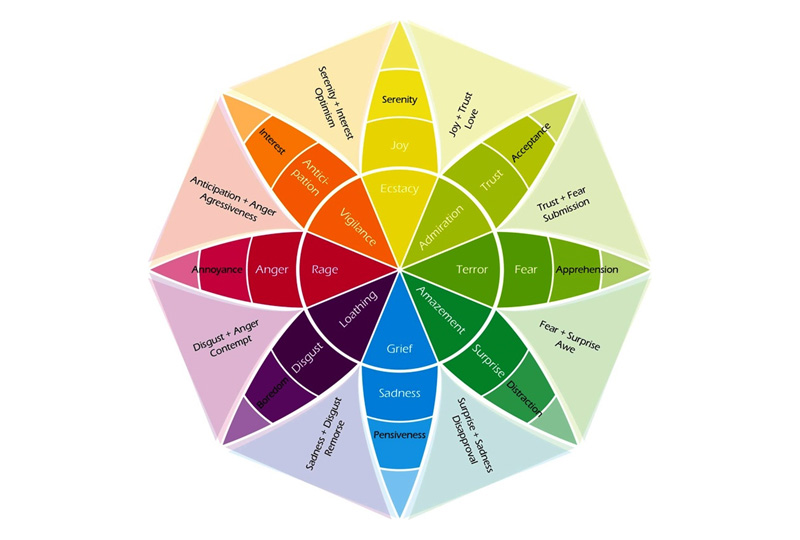
\includegraphics[width=4in]{PlutchikWheelOfEmotion.jpg}
	\label{plutchikemotionwheel}
\end{figure}

\section{Primary Emotion Data}
Table \ref{PrimaryEmotionTable} gives a few examples of the sentences and labeled emotions in the data set which we will call the Primary Emotion data. The Primary Emotion data set contains around $2425$ emotion labeled sentences. For this project the data will be used to develop a model which, when given a text, will assign an emotion to the text. 
 
 \begin{center}
 	\captionof{table}{Primary Emotion Data}
 	\begin{tabular}{ |c|c| } 
 		\hline
 		Emotion & Sentence \\
 		\hline \hline
 		Neutral & Don't let him pick a fight now, we're almost home. \\
 		\hline
 		Optimism &  You must sink your differences. \\
 		\hline
 		Aggression & We'd fight like cat and dog.  \\ 
 		\hline
 		Disgust & For God's sake bury the hatchet. \\
 		\hline
 	\end{tabular}
 	\label{PrimaryEmotionTable}
 \end{center}

 
 Williams hypothesized that the use of idioms in sentiment analysis would increase the accuracy of predicting the correct emotion or category \cite{lowriwilliams}. Figure \ref{topsixgroups} shows a bar plot of the top six emotion groups, ranked by most frequently appearing groups in the data set. The emotion group ``Neutral" occurs the most, it comprises just over $20$ percent of the data set. 
 
% \begin{figure}[h!]
% 	\centering
% 	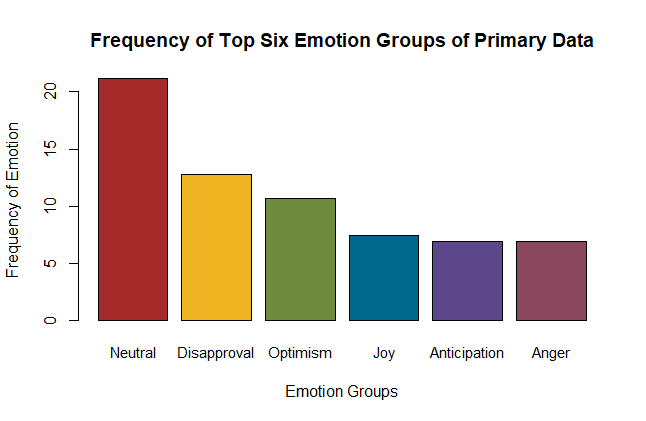
\includegraphics[width = 4.2in]{TopSixGroup1.png}
% 	\caption{Barplot of Frequency of Top Six Emotions in Primary Emotion Data}
% 	\label{TopSixGroup1}
% \end{figure}
 

 \begin{figure}[htb]
		\centering
 		\caption{Frequency of Top Six Emotion Groups in the Primary Emotion Data}
 		% Created by tikzDevice version 0.12 on 2018-12-07 16:26:20
% !TEX encoding = UTF-8 Unicode
\begin{tikzpicture}[x=1pt,y=1pt]
\definecolor{fillColor}{RGB}{255,255,255}
\path[use as bounding box,fill=fillColor,fill opacity=0.00] (0,0) rectangle (361.35,289.08);
\begin{scope}
\path[clip] (  0.00,  0.00) rectangle (361.35,289.08);
\definecolor{drawColor}{RGB}{0,0,0}
\definecolor{fillColor}{RGB}{165,42,42}

\path[draw=drawColor,line width= 0.4pt,line join=round,line cap=round,fill=fillColor] ( 59.83, 62.97) rectangle ( 97.78,239.88);
\definecolor{fillColor}{RGB}{238,180,34}

\path[draw=drawColor,line width= 0.4pt,line join=round,line cap=round,fill=fillColor] (105.38, 62.97) rectangle (143.33,169.98);
\definecolor{fillColor}{RGB}{110,139,61}

\path[draw=drawColor,line width= 0.4pt,line join=round,line cap=round,fill=fillColor] (150.92, 62.97) rectangle (188.88,152.09);
\definecolor{fillColor}{RGB}{0,104,139}

\path[draw=drawColor,line width= 0.4pt,line join=round,line cap=round,fill=fillColor] (196.47, 62.97) rectangle (234.43,124.92);
\definecolor{fillColor}{RGB}{93,71,139}

\path[draw=drawColor,line width= 0.4pt,line join=round,line cap=round,fill=fillColor] (242.02, 62.97) rectangle (279.97,120.95);
\definecolor{fillColor}{RGB}{139,71,93}

\path[draw=drawColor,line width= 0.4pt,line join=round,line cap=round,fill=fillColor] (287.57, 62.97) rectangle (325.52,120.95);
\end{scope}
\begin{scope}
\path[clip] (  0.00,  0.00) rectangle (361.35,289.08);
\definecolor{drawColor}{RGB}{0,0,0}

\node[text=drawColor,anchor=base,inner sep=0pt, outer sep=0pt, scale=  0.80] at ( 78.81, 39.60) {Neutral};

\node[text=drawColor,anchor=base,inner sep=0pt, outer sep=0pt, scale=  0.80] at (124.35, 39.60) {Disapproval};

\node[text=drawColor,anchor=base,inner sep=0pt, outer sep=0pt, scale=  0.80] at (169.90, 39.60) {Optimism};

\node[text=drawColor,anchor=base,inner sep=0pt, outer sep=0pt, scale=  0.80] at (215.45, 39.60) {Joy};

\node[text=drawColor,anchor=base,inner sep=0pt, outer sep=0pt, scale=  0.80] at (261.00, 39.60) {Anticipation};

\node[text=drawColor,anchor=base,inner sep=0pt, outer sep=0pt, scale=  0.80] at (306.54, 39.60) {Anger};
\end{scope}
\begin{scope}
\path[clip] (  0.00,  0.00) rectangle (361.35,289.08);
\definecolor{drawColor}{RGB}{0,0,0}

\node[text=drawColor,anchor=base west,inner sep=0pt, outer sep=0pt, scale=  1.20] at ( 100.00,275.61) {\bfseries Top Six Emotion Groups};

\node[text=drawColor,anchor=base,inner sep=0pt, outer sep=0pt, scale=  1.00] at (192.68, 15.60) {Emotion Groups};

\node[text=drawColor,rotate= 90.00,anchor=base,inner sep=0pt, outer sep=0pt, scale=  1.00] at ( 10.80,150.54) {Frequency of Emotion};
\end{scope}
\begin{scope}
\path[clip] (  0.00,  0.00) rectangle (361.35,289.08);
\definecolor{drawColor}{RGB}{0,0,0}

\path[draw=drawColor,line width= 0.4pt,line join=round,line cap=round] ( 49.20, 62.97) -- ( 49.20,230.21);

\path[draw=drawColor,line width= 0.4pt,line join=round,line cap=round] ( 49.20, 62.97) -- ( 43.20, 62.97);

\path[draw=drawColor,line width= 0.4pt,line join=round,line cap=round] ( 49.20,104.78) -- ( 43.20,104.78);

\path[draw=drawColor,line width= 0.4pt,line join=round,line cap=round] ( 49.20,146.59) -- ( 43.20,146.59);

\path[draw=drawColor,line width= 0.4pt,line join=round,line cap=round] ( 49.20,188.40) -- ( 43.20,188.40);

\path[draw=drawColor,line width= 0.4pt,line join=round,line cap=round] ( 49.20,230.21) -- ( 43.20,230.21);

\node[text=drawColor,rotate= 90.00,anchor=base,inner sep=0pt, outer sep=0pt, scale=  1.00] at ( 34.80, 62.97) {0};

\node[text=drawColor,rotate= 90.00,anchor=base,inner sep=0pt, outer sep=0pt, scale=  1.00] at ( 34.80,104.78) {5};

\node[text=drawColor,rotate= 90.00,anchor=base,inner sep=0pt, outer sep=0pt, scale=  1.00] at ( 34.80,146.59) {10};

\node[text=drawColor,rotate= 90.00,anchor=base,inner sep=0pt, outer sep=0pt, scale=  1.00] at ( 34.80,188.40) {15};

\node[text=drawColor,rotate= 90.00,anchor=base,inner sep=0pt, outer sep=0pt, scale=  1.00] at ( 34.80,230.21) {20};
\end{scope}
\end{tikzpicture}

 		\label{topsixgroups}
 \end{figure}
 	
 %\clearpage
 
\section{Methods}

\subsection{Text Mining}
The goal of this project is to implement a method which when given a bit of text will sort the text into one of the emotions categories. The first step in this project is to do some basic text mining. Text mining is the process of ``cleaning" a data set most raw data will contain punctuation, capitalizations, quotes, tenses, and much more \cite{TextMining}. For most text analysis, not all words are needed. Words like ``the", ``a", ``an", and others, known as ``stopwords", are not important to build a model which will assign emotion or predict a star rating \cite{TextMining}. 

Once the data is clean, each sentence must be broken down into ``tokens". A token can be each sentence, each word, or even a set of words \cite{TextMining}. For this project each token represents a word in each sentence. 

\subsection{Adam Optimizer}

Building on it, the Adam could be viewed as the theoretical successor to RMSProp \cite{adam}. While RMSProp keeps an average square update velocity or `momentum'\cite{rmsprop}, Adam keeps a exponential moving or running average of update velocity squared to control the rate at which the gradient is descended, in which old values are decayed and outweighed by new values \cite{adam}. The original Adam paper justifies this as a `signal to noise ratio'.\cite{adam}.

While theoretically superior, it is sometimes beat out by other optimizers, even its parent optimizer RMSProp. However, the differences are small, and most deficits can be removed by adjusting hyper-parameters. Adam, being theoretically advanced and generally performing well in empirical testing, was chosen as the optimizer for this project. We decisively stuck with it as a matter of practicality \cite{learn}. In this project, our model averaged from ten to twenty minutes to fully train. Hence, we chose to focus on developing one optimizer well, as optimizer to optimizer performance among top contenders don't dramatically differ \cite{learn}.

Algorithm \ref{fig:adam_alg} gives a pseudo-code representation of the Adam optimizer. Refer to Table \cref{fig:adam_table} for an explanation of the components and notation in the description of the optimizer \cite{adam}.

\begin{table}[]
	\begin{adjustwidth}{-1in}{-1in}
		\centering
		\caption{Glossary of notation used in Adam optimizer}
		\label{fig:adam_table}
		\begin{tabular}{lll}
			\hline
			& \textbf{Description}                                                   & \textbf{Elaboration}                                                                                                                                                                                                                                               \\ \hline
			\multicolumn{1}{|l}{$f(x)$}    & Objective function                                                     & \multicolumn{1}{l|}{\begin{tabular}[c]{@{}l@{}}The term to be minimized. This is not the model function.\\ If $g(x)$ is the function we wish to optimize, and $\lambda$ is\\ our loss function, $f(x) = \lambda \circ g(x)$. See eq. 1 \\ for clarification\end{tabular}} \\ \hline
			\multicolumn{1}{|l}{$\alpha$}  & Step Size                                                              & \multicolumn{1}{l|}{Size of increment of change of parameters per $t$.}                                                                                                                                                                                            \\ \hline
			\multicolumn{1}{|l}{$t$}       & Time                                                                   & \multicolumn{1}{l|}{\begin{tabular}[c]{@{}l@{}}Integer value to keep track of iteration of optimizer.\\ Pragmatically, the iterator variable of the optimizer for loop.\end{tabular}}                                                                              \\ \hline
			\multicolumn{1}{|l}{$\odot$}   & Component-Wise Multiplication                                          & \multicolumn{1}{l|}{\begin{tabular}[c]{@{}l@{}}$[a,b,c, ..] \odot [d, e,f,...] = [ad,be,cf,...]$, When a non\\ scalar $n$ value is raised to a power $p$, it implies\\  $n \odot n^{p-1}$\end{tabular}}                                                                      \\ \hline
			\multicolumn{1}{|l}{$m_t$}     & Moment  Estimation                                                     & \multicolumn{1}{l|}{\begin{tabular}[c]{@{}l@{}}Moving average of gradient -- a smoothed version of\\ the gradient function. Defined by first moment of \\ gradient.\end{tabular}}                                                                                  \\ \hline
			\multicolumn{1}{|l}{$v_t$}     & Variance Estimation                                                    & \multicolumn{1}{l|}{\begin{tabular}[c]{@{}l@{}}Variance of gradient function as defined by second\\  moment of gradient.\end{tabular}}                                                                                                                             \\ \hline
			\multicolumn{1}{|l}{$\theta$}  & \begin{tabular}[c]{@{}l@{}}Parameters of Model\\ Function\end{tabular} & \multicolumn{1}{l|}{Parameters of model. Earlier denoted $p$ and $m$.}                                                                                                                                                                                             \\ \hline
			\multicolumn{1}{|l}{$g_t$}     & Gradient                                                               & \multicolumn{1}{l|}{\begin{tabular}[c]{@{}l@{}}Gradient with respect to optimization parameters. \\ Earlier denoted  $\frac{\partial \lambda}{\partial p}$, more appropriately denoted $\nabla_\theta f(\theta)$\end{tabular}}                                   \\ \hline
			\multicolumn{1}{|l}{$\beta_1$} & Decay rate of $m_t$                                                    & \multicolumn{1}{l|}{\begin{tabular}[c]{@{}l@{}}Multiplied by previous $m_t$ each iteration($t$),  \\ and determines how long back to find average gradient.\\ \\ Acceptable range [0,1), Default .9\end{tabular}}                                                                           \\ \hline
			\multicolumn{1}{|l}{$\beta_2$} & Decay rate of $v_t$                                                    & \multicolumn{1}{l|}{\begin{tabular}[c]{@{}l@{}}Multiplied by previous $v_t$ each iteration($t$), \\ and determines how long back to calculate moving variance.  \\ \\ Acceptable range: [0,1), Default .999\end{tabular}}                                                                           \\ \hline
		\end{tabular}
	\end{adjustwidth}
\end{table}

\newcommand{\assn}{\mathrel{{:}{=}}}

\begin{algorithm}[]
	\KwData{$\theta_0$, $f(x)$ (initial function parameters, unoptimized objective function), }
	\textbf{Initialize variables}:
	$\{m_0,V_0,t\} = 0$\;
	\vspace{3.5mm}
	\While{\text{model is not fitted}}{
		\begin{align*}
		t &\assn t +  1\\ 
		g_t &\assn \nabla_\theta f\left(\theta_{t-1}\right)\;  \hspace{2mm} \text{Find actual gradient. }\\
		m_t &\assn \beta_1 m_{t-1} + (1-\beta_1)g_t\\
		&\text{Assign new gradient moving average, where previous} \\
		&\text{gradients have weight} \frac{\beta_1}{1} \\
		v_t &\assn \beta_2 m_{t-1} + (1-\beta_1)g_t^2 \\
		&\text{Assign a new moving variance estimation in the same manner,}\\
		&\text{but instead using } \beta_2\\
		\widehat{m_t} &\assn \frac{m_t}{1-\beta_1^t}\\
		\widehat{v_t} &\assn \frac{v_t}{1-\beta_2^t}\\
		&\text{Bias results from where we initiated } v_t \text{ with zero. The last two}\\
		&\text{statements correct that bias. See Adam paper.}\\
		\theta_t &\assn \theta_{t-1} - \alpha\frac{ \widehat{m_t}}{\sqrt{v_t} + \epsilon}\\
		& \text{Update the parameters going in the opposite direction of our new}\\
		& \text{calculated gradient average. Weigh update by dividing by } \sqrt{\widehat{v_t}}, \\
		& \text{(more noise, lower effective step size.)}
		\end{align*}
	}
	\vspace{3.5mm}
	\caption{Pseudo-code representation of Adam optimizer. The $\mathrel{{:}{=}}$ ligature  represents assignment.}
	\label{fig:adam_alg}
\end{algorithm}

\subsubsection{Further Comments on Components}

%Richard, Dr. Joyner doesn't think this paragraph flows with the rest of the paper, do you think you could maybe add a transition or something here?

%Dr. Joyner could be having a problem with this paragraph because it's appearing between the algorithm and the table explaining the algorithm..

\paragraph{Gradient} - The gradient of a function $\nabla_\theta f(\theta)$ evaluated at point $\theta$ is by definition the direction of steepest ascent at point $\theta$. We use this, as we are trying to reduce our inaccuracy/loss by moving in the direction of steepest \textit{descent} \mbox{(i.e. $-\nabla_\theta f(\theta)$)}. \cite{gradient} 

\paragraph{Gradient Moving Average}
The Adam optimizer does not just naively use the gradient itself, but instead smooths it using the exponential moving average as originally described by J. Stuart Hunter.\cite{EMA} This formula gives a much less noisy curve to descend, and helps prevent the optimizer from plateauing in local minima. Although used recursively here, a non recursive equivalent is given by
\[m_t = \sum_{t=0}^{t_f} \left(1-\beta_1\right) \beta_1^{t_f-t}\nabla_\theta f\left(\theta_{t}\right)^2\].
(Although purely semantic, in the original EMA formula, \(\beta_1\) and and \(\left(1-\beta_1\right)\) are switched.)

\paragraph{Moving Variance}
The moving variance is used to modulate the learning rate of the function, depending on how noisy the slope is. For an intuitive sense, 
recall that standard deviation is given by
\[\sigma = \sqrt{\sum \left(x_n - \bar{x}\right)^2}\].
If we replace \(x_n\) with \ \(\nabla_\theta f(\theta)\), and \(\bar{x}\) with a gradient of \(\vec{0}\), we get \footnote{\(f\left(\theta_{t}\right)^2 \implies \) component wise multiplication}
\[\sigma = \sqrt{\sum \left(\nabla_\theta f(\theta)\right)^2}\].
Applying the same exponential moving average to this `variance from the zero gradient' yields a moving average in the same manner of the moving average of the gradient. Albeit, the variance is more conservative, as \(\beta_2\) is typically larger than \(\beta_1\)\cite{adam}.

\subsection{Model Layers}

Although earlier referred to as the objective function, the predictive model is not actually a single function, but instead a composition of functions. Each element function is henceforth referred to as a layer. Diagrammed in \cref{layers}, our model is composed of three main layers: an embedding layer, a single or multiple (Bi-)LSTM layer(s), and a dense output layer.

Data is transported through the layers in tensors\cite{tensorflow}. Tensors are a generalization of linear algebra, matrices and vectors to higher dimensions. The essentials are that, a rank zero tensor is a scalar, a rank one tensor is a vector, rank two is a matrix, and three is a `three dimensional' matrix, and so on \cite{tensors}. 

\begin{figure}[h]
	\centering
	\caption{Model Layers with Data Flow and Back Propagation of Updates \cite{knisely}}
	\label{layers}
	\def\svgwidth{3.5in}
	%LaTeX with PSTricks extensions
%%Creator: inkscape 0.92.2
%%Please note this file requires PSTricks extensions
\psset{xunit=.5pt,yunit=.5pt,runit=.5pt}
\begin{pspicture}(453.54330444,340.1574707)
{
\newrgbcolor{curcolor}{0 0 0}
\pscustom[linewidth=1,linecolor=curcolor]
{
\newpath
\moveto(133.1811,285.6284097)
\lineto(133.1811,151.1811007)
}
}
{
\newrgbcolor{curcolor}{0 0 0}
\pscustom[linewidth=1,linecolor=curcolor]
{
\newpath
\moveto(133.1811,151.1811007)
\lineto(170.97638,151.1811007)
\lineto(170.97638,285.6284097)
\lineto(133.1811,285.6284097)
}
}
{
\newrgbcolor{curcolor}{0 0 0}
\pscustom[linestyle=none,fillstyle=solid,fillcolor=curcolor]
{
\newpath
\moveto(85.40369873,218.94577728)
\lineto(84.57579344,218.92670236)
\lineto(84.54160255,220.41068353)
\lineto(74.54425569,220.18034488)
\lineto(74.57844659,218.69636371)
\lineto(73.74273087,218.67710884)
\lineto(73.52642848,228.06524236)
\lineto(76.11949032,228.12498645)
\lineto(76.14162443,227.1643039)
\lineto(74.50924514,227.12669392)
\lineto(74.63269226,221.76874084)
\lineto(78.53790587,221.85871688)
\lineto(78.44990931,225.67801579)
\lineto(76.98935942,225.64436476)
\lineto(76.96722531,226.6050473)
\lineto(80.84119722,226.69430353)
\lineto(80.86333132,225.73362098)
\lineto(79.40278143,225.69996995)
\lineto(79.490778,221.88067103)
\lineto(84.37229501,221.99314108)
\lineto(84.24596866,227.47606099)
\lineto(82.61358937,227.43845101)
\lineto(82.59145526,228.39913356)
\lineto(85.1845171,228.45887765)
\closepath
}
}
{
\newrgbcolor{curcolor}{0 0 0}
\pscustom[linestyle=none,fillstyle=solid,fillcolor=curcolor]
{
\newpath
\moveto(85.13970904,230.40367403)
\lineto(84.31180375,230.38459911)
\lineto(84.28193171,231.68113003)
\lineto(77.64306856,231.52817076)
\lineto(77.67474013,230.15353557)
\lineto(76.83902441,230.1342807)
\lineto(76.77424167,232.9460345)
\lineto(78.25041241,232.98004544)
\curveto(77.68194328,233.23264342)(77.24965884,233.56652482)(76.9535591,233.98168965)
\curveto(76.65733939,234.40206143)(76.50275126,234.8934227)(76.48979471,235.45577346)
\curveto(76.46868033,236.37219692)(76.71609552,237.05255553)(77.23204027,237.49684927)
\curveto(77.74798502,237.94114302)(78.56310121,238.17612647)(79.67738883,238.20179963)
\lineto(84.12933235,238.30437232)
\lineto(84.09982021,239.58528238)
\lineto(84.92772549,239.6043573)
\lineto(85.01914115,235.63666027)
\lineto(84.19123586,235.61758535)
\lineto(84.16262348,236.85944328)
\lineto(80.16368474,236.76730782)
\curveto(79.1483292,236.74391405)(78.45608041,236.60293148)(78.08693837,236.34436011)
\curveto(77.71258938,236.08566877)(77.53267295,235.64130253)(77.54718908,235.0112614)
\curveto(77.56254499,234.34477161)(77.8189686,233.84273234)(78.3164599,233.50514359)
\curveto(78.80874424,233.16743487)(79.52090857,233.00931765)(80.45295289,233.03079193)
\lineto(84.24882052,233.11824864)
\lineto(84.22002819,234.36791699)
\lineto(85.04793348,234.38699191)
\closepath
}
}
{
\newrgbcolor{curcolor}{0 0 0}
\pscustom[linestyle=none,fillstyle=solid,fillcolor=curcolor]
{
\newpath
\moveto(77.25707136,248.28153717)
\lineto(84.54419997,248.44943245)
\curveto(85.73659186,248.47690514)(86.66317678,248.17004155)(87.32395474,247.52884171)
\curveto(87.98993965,246.88776182)(88.33690838,245.96061204)(88.36486094,244.74739234)
\curveto(88.37745758,244.20066243)(88.34004833,243.67622411)(88.25263319,243.17407738)
\curveto(88.16521804,242.67193064)(88.02785699,242.18947202)(87.84055002,241.7267015)
\lineto(86.09882475,241.68657219)
\lineto(86.08154935,242.4363732)
\curveto(86.62091288,242.542575)(87.01154255,242.77298801)(87.25343836,243.12761223)
\curveto(87.49533417,243.48223645)(87.60878407,243.98498302)(87.59378807,244.63585196)
\curveto(87.57435324,245.4793781)(87.32061726,246.09088332)(86.83258012,246.47036762)
\curveto(86.34962997,246.85517884)(85.59787364,247.03582758)(84.57731115,247.01231384)
\lineto(83.46042006,246.9865807)
\curveto(83.98759348,246.71740212)(84.38118568,246.36700011)(84.64119667,245.93537465)
\curveto(84.89588074,245.50883617)(85.03060081,244.97533942)(85.04535688,244.33488439)
\curveto(85.06887062,243.31432189)(84.68458675,242.46930866)(83.89250527,241.79984467)
\curveto(83.09509688,241.13546767)(82.04552375,240.78828317)(80.74378588,240.75829116)
\curveto(79.442048,240.72829914)(78.38020231,241.02683661)(77.55824879,241.65390354)
\curveto(76.73629527,242.28097048)(76.31350166,243.10738867)(76.28986796,244.13315811)
\curveto(76.27511189,244.77361314)(76.38772201,245.31280838)(76.62769834,245.75074382)
\curveto(76.86234774,246.19376624)(77.23678088,246.56186355)(77.75099775,246.85503573)
\lineto(76.45446683,246.82516369)
\lineto(76.38968409,249.63691749)
\lineto(77.2253998,249.65617236)
\closepath
\moveto(80.19566147,246.91136073)
\curveto(79.20113374,246.88844683)(78.44535764,246.67827429)(77.92833318,246.28084311)
\curveto(77.41118874,245.88861888)(77.16101429,245.32802016)(77.17780982,244.59904695)
\curveto(77.19484528,243.85965984)(77.49933113,243.30663077)(78.09126736,242.93995973)
\curveto(78.68308363,242.57849564)(79.5543599,242.41102007)(80.70509618,242.43753301)
\curveto(81.85062551,242.46392598)(82.71326408,242.67135091)(83.2930119,243.05980781)
\curveto(83.87263975,243.45347166)(84.15393594,244.01999714)(84.13690048,244.75938425)
\curveto(84.12010495,245.48835746)(83.84698078,246.03689939)(83.31752796,246.40501004)
\curveto(82.78274823,246.77820768)(82.01549102,246.95328956)(81.01575633,246.9302557)
\closepath
}
}
{
\newrgbcolor{curcolor}{0 0 0}
\pscustom[linestyle=none,fillstyle=solid,fillcolor=curcolor]
{
\newpath
\moveto(83.777706,253.56594712)
\lineto(83.74639434,254.92496146)
\lineto(84.57429962,254.94403638)
\lineto(84.67057398,250.76545781)
\lineto(83.84266869,250.74638289)
\lineto(83.81081718,252.12882851)
\lineto(73.31360298,251.88697293)
\lineto(73.3454545,250.50452731)
\lineto(72.51754921,250.48545239)
\lineto(72.45258651,253.30501662)
\closepath
}
}
{
\newrgbcolor{curcolor}{0 0 0}
\pscustom[linestyle=none,fillstyle=solid,fillcolor=curcolor]
{
\newpath
\moveto(73.647407,256.73188465)
\curveto(73.40788723,256.72636612)(73.1976297,256.8074821)(73.0166344,256.97523258)
\curveto(72.83551914,257.14819002)(72.74214226,257.3570321)(72.73650376,257.60175882)
\curveto(72.73098523,257.84127858)(72.81476467,258.04899262)(72.98784207,258.22490094)
\curveto(73.16079951,258.4060162)(73.36703811,258.4993331)(73.60655788,258.50485163)
\curveto(73.8512846,258.51049013)(74.06154213,258.42937415)(74.23733048,258.2615037)
\curveto(74.41311882,258.09363324)(74.50383224,257.88733466)(74.50947074,257.64260794)
\curveto(74.51510924,257.39788122)(74.43405325,257.18502021)(74.26630276,257.00402491)
\curveto(74.09843231,256.82823657)(73.89213372,256.73752315)(73.647407,256.73188465)
\closepath
\moveto(83.65713811,258.79893337)
\lineto(83.62582645,260.1579477)
\lineto(84.45373173,260.17702262)
\lineto(84.54982614,256.00625448)
\lineto(83.72192085,255.98717956)
\lineto(83.69024929,257.36181476)
\lineto(77.05138614,257.20885549)
\lineto(77.08305771,255.8342203)
\lineto(76.247342,255.81496543)
\lineto(76.18255925,258.62671923)
\closepath
}
}
{
\newrgbcolor{curcolor}{0 0 0}
\pscustom[linestyle=none,fillstyle=solid,fillcolor=curcolor]
{
\newpath
\moveto(83.96358434,261.43950509)
\lineto(82.02659839,261.39487697)
\lineto(82.00752347,262.22278226)
\curveto(82.62667082,262.25788626)(83.08565068,262.46122063)(83.38446306,262.83278535)
\curveto(83.68315547,263.20955702)(83.82422387,263.7572225)(83.80766828,264.47578181)
\curveto(83.79279224,265.12144379)(83.66169538,265.61074144)(83.41437769,265.94367476)
\curveto(83.16185304,266.27648811)(82.80388138,266.4375562)(82.3404627,266.42687905)
\curveto(81.9759761,266.41848128)(81.68466257,266.28673625)(81.46652212,266.03164396)
\curveto(81.24826171,265.78175861)(81.02073874,265.25554493)(80.78395323,264.45300292)
\lineto(80.45641763,263.40611825)
\curveto(80.24374739,262.68748731)(79.96930188,262.16279739)(79.6330811,261.83204851)
\curveto(79.29674035,261.50650658)(78.86301545,261.33761724)(78.3319064,261.3253805)
\curveto(77.57169148,261.30786516)(76.96907725,261.57270073)(76.52406369,262.11988719)
\curveto(76.07905014,262.66707365)(75.84520638,263.43272379)(75.82253242,264.41683763)
\curveto(75.8124551,264.85422155)(75.8591144,265.31635641)(75.9625103,265.80324219)
\curveto(76.06590621,266.29012798)(76.22101172,266.7938343)(76.42782685,267.31436115)
\lineto(78.23984596,267.35611003)
\lineto(78.25892088,266.52820475)
\curveto(77.72308475,266.49502023)(77.30824401,266.29791255)(77.01439865,265.9368817)
\curveto(76.72055329,265.57585085)(76.58064874,265.09072877)(76.594685,264.48151544)
\curveto(76.6086013,263.87750907)(76.72590099,263.42175669)(76.94658409,263.11425829)
\curveto(77.16714721,262.81196684)(77.49091379,262.6657398)(77.91788381,262.67557718)
\curveto(78.26674956,262.68361504)(78.54522566,262.80724973)(78.7533121,263.04648123)
\curveto(78.9561916,263.28559277)(79.15887949,263.7591371)(79.36137576,264.46711421)
\lineto(79.68657199,265.61553442)
\curveto(79.91318353,266.4074226)(80.20737714,266.97945495)(80.5691528,267.33163148)
\curveto(80.92560154,267.68889499)(81.39281172,267.87418497)(81.97078334,267.88750143)
\curveto(82.75703301,267.9056166)(83.38361839,267.61788961)(83.85053946,267.02432046)
\curveto(84.31213361,266.43583829)(84.55510745,265.61309163)(84.57946096,264.55608048)
\curveto(84.59181767,264.01976448)(84.54659799,263.49514621)(84.44380193,262.98222566)
\curveto(84.34100587,262.46930512)(84.18093333,261.95506493)(83.96358434,261.43950509)
\closepath
}
}
{
\newrgbcolor{curcolor}{0 0 0}
\pscustom[linestyle=none,fillstyle=solid,fillcolor=curcolor]
{
\newpath
\moveto(84.24066848,269.42456846)
\lineto(83.41276319,269.40549354)
\lineto(83.38289115,270.70202446)
\lineto(72.88567695,270.46016888)
\lineto(72.91734852,269.08553368)
\lineto(72.08944323,269.06645876)
\lineto(72.02466048,271.87821257)
\lineto(77.35137185,272.00093988)
\curveto(76.78290272,272.25353786)(76.35061829,272.58741926)(76.05451854,273.00258409)
\curveto(75.75829883,273.42295587)(75.6037107,273.91431714)(75.59075415,274.4766679)
\curveto(75.56963977,275.39309136)(75.81705496,276.07344996)(76.33299971,276.51774371)
\curveto(76.84894447,276.96203745)(77.66406065,277.19702091)(78.77834827,277.22269407)
\lineto(83.23029179,277.32526675)
\lineto(83.20077965,278.60617682)
\lineto(84.02868494,278.62525174)
\lineto(84.12010059,274.65755471)
\lineto(83.2921953,274.63847979)
\lineto(83.26358292,275.88033772)
\lineto(79.26464418,275.78820225)
\curveto(78.24928864,275.76480848)(77.55964333,275.6238859)(77.19570824,275.3654345)
\curveto(76.82644623,275.11207008)(76.64913328,274.66776383)(76.66376938,274.03251574)
\curveto(76.67912529,273.36602595)(76.93294542,272.8639267)(77.42522976,272.52621798)
\curveto(77.91751411,272.18850926)(78.62707497,272.03033205)(79.55391233,272.05168637)
\lineto(83.34977997,272.13914307)
\lineto(83.32098763,273.38881143)
\lineto(84.14889292,273.40788635)
\closepath
}
}
{
\newrgbcolor{curcolor}{0 0 0}
\pscustom[linestyle=none,fillstyle=solid,fillcolor=curcolor]
{
\newpath
\moveto(83.8305577,287.22453212)
\lineto(83.00265242,287.2054572)
\lineto(82.96828157,288.6972488)
\lineto(73.06465984,288.46906957)
\lineto(73.1436588,285.04029202)
\lineto(74.96348835,285.08222085)
\lineto(74.98562245,284.1215383)
\lineto(72.23635207,284.05819517)
\lineto(71.99773562,294.41482168)
\lineto(74.747006,294.47816481)
\lineto(74.76914011,293.51748226)
\lineto(72.94931057,293.47555342)
\lineto(73.02830953,290.04677587)
\lineto(82.93193125,290.2749551)
\lineto(82.89756041,291.7667467)
\lineto(83.72546569,291.78582162)
\closepath
}
}
{
\newrgbcolor{curcolor}{0 0 0}
\pscustom[linestyle=none,fillstyle=solid,fillcolor=curcolor]
{
\newpath
\moveto(79.48485132,302.18308993)
\lineto(79.62755331,295.98942113)
\lineto(79.69003673,295.99086075)
\curveto(80.8095313,296.01665388)(81.65080221,296.24703022)(82.21384946,296.68198978)
\curveto(82.77168976,297.11682937)(83.04113243,297.74559833)(83.02217748,298.56829666)
\curveto(83.00766135,299.19833779)(82.83176554,299.710047)(82.49449006,300.10342427)
\curveto(82.15188765,300.50188853)(81.65329248,300.77433041)(80.99870453,300.9207499)
\lineto(80.97207163,302.07669313)
\curveto(81.88856673,301.86858167)(82.58305825,301.45999093)(83.05554618,300.85092089)
\curveto(83.52791414,300.2470578)(83.77567503,299.44265544)(83.79882887,298.4377138)
\curveto(83.82678142,297.22449411)(83.45094364,296.23901315)(82.67131553,295.48127092)
\curveto(81.8863605,294.72861568)(80.83260014,294.33705212)(79.51003446,294.30658024)
\curveto(78.19788269,294.27634829)(77.13253376,294.6138779)(76.31398767,295.31916908)
\curveto(75.49544158,296.02446026)(75.07261215,296.96549136)(75.04549937,298.1422624)
\curveto(75.01658707,299.39713771)(75.38231087,300.36936135)(76.14267076,301.05893333)
\curveto(76.8978237,301.74838535)(78.01188389,302.12310421)(79.48485132,302.18308993)
\closepath
\moveto(78.69599563,300.4691523)
\curveto(77.72822246,300.41559653)(77.00398799,300.19312642)(76.52329222,299.80174197)
\curveto(76.03726953,299.41544449)(75.80241601,298.86822306)(75.81873166,298.16007766)
\curveto(75.83396761,297.49879482)(76.09329461,296.98379815)(76.59671267,296.61508766)
\curveto(77.10013072,296.24637716)(77.83444251,296.03146335)(78.79964802,295.97034621)
\closepath
}
}
{
\newrgbcolor{curcolor}{0 0 0}
\pscustom[linestyle=none,fillstyle=solid,fillcolor=curcolor]
{
\newpath
\moveto(78.28921624,307.6101147)
\lineto(75.85128577,309.29659468)
\lineto(75.87701891,308.17970359)
\lineto(75.0413032,308.16044872)
\lineto(74.9677028,311.35491346)
\lineto(75.80341852,311.37416833)
\lineto(75.82879176,310.27289809)
\lineto(78.949576,308.11764749)
\lineto(82.45919716,310.79294743)
\lineto(82.43418382,311.87859681)
\lineto(83.2620891,311.89767173)
\lineto(83.35044557,308.06275196)
\lineto(82.52254029,308.04367704)
\lineto(82.49824676,309.09808472)
\lineto(80.05609983,307.23665127)
\lineto(82.58156457,305.48185691)
\lineto(82.55673118,306.55969587)
\lineto(83.38463647,306.57877079)
\lineto(83.4573371,303.42335819)
\lineto(82.62943182,303.40428327)
\lineto(82.60405857,304.50555351)
\lineto(79.39592002,306.72130805)
\lineto(75.97059399,304.11828143)
\lineto(75.99416771,303.09511546)
\lineto(75.158452,303.07586059)
\lineto(75.07297477,306.78581353)
\lineto(75.90869048,306.8050684)
\lineto(75.93154439,305.81314414)
\closepath
}
}
{
\newrgbcolor{curcolor}{0 0 0}
\pscustom[linestyle=none,fillstyle=solid,fillcolor=curcolor]
{
\newpath
\moveto(75.75087251,313.65481308)
\lineto(75.78002475,312.38952387)
\lineto(74.94430903,312.37026899)
\lineto(74.9151568,313.63555821)
\lineto(72.33771581,313.57617402)
\lineto(72.30442468,315.02110306)
\lineto(74.88186566,315.08048724)
\lineto(74.81960225,317.78289506)
\lineto(75.65531796,317.80214994)
\lineto(75.71758138,315.09974212)
\lineto(80.98961976,315.22120976)
\curveto(81.69255821,315.23740545)(82.14139993,315.31547306)(82.33614491,315.45541258)
\curveto(82.5308899,315.59535211)(82.62406351,315.84756517)(82.61566575,316.21205177)
\curveto(82.60702805,316.58695228)(82.49138375,316.8577979)(82.26873284,317.02458865)
\curveto(82.04087498,317.19125942)(81.67949588,317.27410327)(81.18459556,317.27312021)
\lineto(81.15958222,318.3587696)
\curveto(81.91554993,318.33450935)(82.47222552,318.14155138)(82.82960901,317.77989569)
\curveto(83.18699249,317.41823999)(83.37438191,316.85990816)(83.39177728,316.10490019)
\curveto(83.4108522,315.27699491)(83.2421053,314.68701398)(82.88553659,314.33495742)
\curveto(82.52376092,313.98278089)(81.90288569,313.79655533)(81.02291089,313.77628073)
\closepath
}
}
{
\newrgbcolor{curcolor}{0 0 0}
\pscustom[linestyle=none,fillstyle=solid,fillcolor=curcolor]
{
\newpath
\moveto(156.96803038,174.23562293)
\lineto(156.14005306,174.21998412)
\lineto(156.11202124,175.70409441)
\lineto(146.11380454,175.51524845)
\lineto(146.14183636,174.03113816)
\lineto(145.30604793,174.01535182)
\lineto(145.12870977,183.40430219)
\lineto(147.72199722,183.45328411)
\lineto(147.74014414,182.49251797)
\lineto(146.10762282,182.46168297)
\lineto(146.20883246,177.1032637)
\lineto(150.11438585,177.17703166)
\lineto(150.04224079,180.99666288)
\lineto(148.58156382,180.96907367)
\lineto(148.56341691,181.9298398)
\lineto(152.43772588,182.00301762)
\lineto(152.45587279,181.04225148)
\lineto(150.99519582,181.01466226)
\lineto(151.06734088,177.19503104)
\lineto(155.94928263,177.28724098)
\lineto(155.84571242,182.77063796)
\lineto(154.2131911,182.73980295)
\lineto(154.19504419,183.70056909)
\lineto(156.78833164,183.74955101)
\closepath
}
}
{
\newrgbcolor{curcolor}{0 0 0}
\pscustom[linestyle=none,fillstyle=solid,fillcolor=curcolor]
{
\newpath
\moveto(149.9211452,193.1996772)
\curveto(149.30666593,193.46416184)(148.84177522,193.80700621)(148.52647305,194.2282103)
\curveto(148.20586513,194.65452344)(148.04015151,195.15408726)(148.02933221,195.72690176)
\curveto(148.01290655,196.59653832)(148.2714461,197.24997476)(148.80495088,197.68721109)
\curveto(149.33324825,198.12434906)(150.14157071,198.35319638)(151.22991826,198.37375305)
\lineto(155.68224913,198.45784852)
\lineto(155.65775817,199.75449224)
\lineto(156.48573549,199.77013105)
\lineto(156.5609788,195.78646658)
\lineto(155.73300148,195.77082778)
\lineto(155.70939574,197.02060487)
\lineto(151.42109811,196.93960765)
\curveto(150.57229117,196.92357542)(149.97059282,196.78718826)(149.61600305,196.53044619)
\curveto(149.26141329,196.27370412)(149.08957724,195.85632214)(149.10049489,195.27830024)
\curveto(149.11259284,194.63778948)(149.36398273,194.15286706)(149.85466458,193.823533)
\curveto(150.34524806,193.49940633)(151.05399881,193.3460968)(151.98091682,193.36360439)
\lineto(155.77711472,193.43530685)
\lineto(155.75350898,194.68508393)
\lineto(156.5814863,194.70072274)
\lineto(156.65584439,190.76392491)
\lineto(155.82786707,190.74828611)
\lineto(155.80426133,191.99806319)
\lineto(151.46128595,191.91603323)
\curveto(150.63330863,191.90039442)(150.04723249,191.76430234)(149.70305754,191.50775699)
\curveto(149.35367518,191.25111327)(149.18444283,190.83378047)(149.19536048,190.25575856)
\curveto(149.20745843,189.61524781)(149.45884832,189.13032539)(149.94953017,188.80099133)
\curveto(150.44011365,188.47686466)(151.1488644,188.32355513)(152.07578241,188.34106272)
\lineto(155.87198031,188.41276517)
\lineto(155.84837457,189.66254226)
\lineto(156.67635189,189.67818107)
\lineto(156.7515952,185.6945166)
\lineto(155.92361788,185.6788778)
\lineto(155.89912692,186.97552152)
\lineto(149.24406393,186.84982093)
\lineto(149.27003025,185.47506613)
\lineto(148.44986403,185.45957486)
\lineto(148.39675111,188.27157331)
\lineto(149.87305029,188.2994576)
\curveto(149.31604919,188.55460936)(148.8878562,188.88512371)(148.58847132,189.29100066)
\curveto(148.28908644,189.69687761)(148.13447614,190.16018631)(148.12464041,190.68092677)
\curveto(148.11244411,191.32664493)(148.26369367,191.86866037)(148.5783891,192.3069731)
\curveto(148.88787712,192.74518747)(149.33546249,193.04275551)(149.9211452,193.1996772)
\closepath
}
}
{
\newrgbcolor{curcolor}{0 0 0}
\pscustom[linestyle=none,fillstyle=solid,fillcolor=curcolor]
{
\newpath
\moveto(155.61438261,202.05095764)
\lineto(145.11625508,201.85266938)
\lineto(145.14236893,200.47010348)
\lineto(144.31439161,200.45446467)
\lineto(144.26113115,203.27427422)
\lineto(149.40865053,203.37150039)
\curveto(148.88259878,203.64286451)(148.49311708,203.99234246)(148.24020541,204.41993424)
\curveto(147.98198798,204.85263507)(147.84683029,205.38924087)(147.83473235,206.02975163)
\curveto(147.81545432,207.05040291)(148.20329101,207.89121033)(148.99824241,208.55217387)
\curveto(149.79319381,209.21313741)(150.84159508,209.55591383)(152.14344621,209.58050315)
\curveto(153.44529734,209.60509247)(154.50849862,209.30219992)(155.33305002,208.67182549)
\curveto(156.15239403,208.04135271)(156.57170504,207.21579067)(156.59098307,206.19513938)
\curveto(156.60308101,205.55462862)(156.49088699,205.01335086)(156.25440098,204.57130609)
\curveto(156.01260922,204.13437036)(155.63399876,203.77038471)(155.1185696,203.47934914)
\lineto(156.41521333,203.5038401)
\lineto(156.46847379,200.68403055)
\lineto(155.64049647,200.66839174)
\closepath
\moveto(152.67369317,203.4331704)
\curveto(153.67351484,203.452055)(154.43280956,203.6565346)(154.95157734,204.04660922)
\curveto(155.46503935,204.44179288)(155.71488535,205.00390303)(155.70111533,205.73293966)
\curveto(155.68724696,206.4671837)(155.38255355,207.0162151)(154.78703512,207.38003385)
\curveto(154.19141832,207.74906001)(153.32079543,207.92275379)(152.17516643,207.90111519)
\curveto(151.02433003,207.87937823)(150.16088722,207.67293148)(149.58483799,207.28177494)
\curveto(149.00869041,206.8958258)(148.7275508,206.33572921)(148.74141918,205.60148517)
\curveto(148.7551892,204.87244853)(149.02868735,204.32022329)(149.56191365,203.94480944)
\curveto(150.09504159,203.57460299)(150.85891269,203.39889289)(151.85352696,203.41767913)
\closepath
}
}
{
\newrgbcolor{curcolor}{0 0 0}
\pscustom[linestyle=none,fillstyle=solid,fillcolor=curcolor]
{
\newpath
\moveto(152.12055975,219.06613752)
\lineto(152.23755573,212.87192983)
\lineto(152.30004458,212.87311012)
\curveto(153.41963656,212.89425693)(154.26185632,213.12113987)(154.82670388,213.55375894)
\curveto(155.38634404,213.98627965)(155.65839389,214.61392496)(155.64285344,215.43669488)
\curveto(155.63095221,216.06679083)(155.4571816,216.57922562)(155.1215416,216.97399926)
\curveto(154.78059585,217.37388195)(154.28313565,217.64839074)(153.62916101,217.79752562)
\lineto(153.60732569,218.95356942)
\curveto(154.5229492,218.74165615)(155.21573902,218.33018666)(155.68569513,217.71916096)
\curveto(156.15555289,217.11334267)(156.39997324,216.30791898)(156.4189562,215.30288991)
\curveto(156.44187344,214.08956465)(156.06194898,213.10565197)(155.27918282,212.35115186)
\curveto(154.4911109,211.6017608)(153.43573457,211.2145739)(152.11305381,211.18959115)
\curveto(150.80078787,211.16480512)(149.73684892,211.50675321)(148.92123696,212.21543542)
\curveto(148.105625,212.92411763)(147.68670465,213.86689545)(147.66447591,215.04376887)
\curveto(147.64077181,216.29875336)(148.01052735,217.26945082)(148.77374253,217.95586124)
\curveto(149.53175032,218.6421733)(150.64735606,219.01226539)(152.12055975,219.06613752)
\closepath
\moveto(151.32459772,217.35548854)
\curveto(150.35661063,217.30594966)(149.6314591,217.08648716)(149.14914316,216.69710105)
\curveto(148.66152145,216.31282398)(148.42439889,215.76658194)(148.43777548,215.05837492)
\curveto(148.45026686,214.39703455)(148.7074543,213.88096607)(149.20933781,213.51016948)
\curveto(149.71122132,213.13937289)(150.44463485,212.9214134)(151.40957841,212.85629103)
\closepath
}
}
{
\newrgbcolor{curcolor}{0 0 0}
\pscustom[linestyle=none,fillstyle=solid,fillcolor=curcolor]
{
\newpath
\moveto(155.11821935,228.3197098)
\lineto(155.09225303,229.6944646)
\lineto(155.92023035,229.71010341)
\lineto(155.97334327,226.89810496)
\lineto(154.67669955,226.873614)
\curveto(155.20275129,226.60224988)(155.59488588,226.25021741)(155.85310331,225.81751658)
\curveto(156.10601497,225.38992479)(156.23851978,224.85587352)(156.25061772,224.21536276)
\curveto(156.26989575,223.19471147)(155.88210824,222.35130036)(155.0872552,221.68512941)
\curveto(154.28709639,221.02406752)(153.23609142,220.68124191)(151.93424029,220.65665259)
\curveto(150.63238916,220.63206327)(149.57179159,220.93500501)(148.75244759,221.56547779)
\curveto(147.93310358,222.19595058)(147.51374339,223.02411631)(147.494367,224.04997501)
\curveto(147.48226906,224.69048577)(147.59711597,225.22920901)(147.83890773,225.66614473)
\curveto(148.07539374,226.1081895)(148.45135132,226.47472968)(148.96678048,226.76576525)
\lineto(144.64723842,226.68417789)
\lineto(144.67290967,225.32504531)
\lineto(143.84493235,225.3094065)
\lineto(143.79211449,228.10578273)
\closepath
\moveto(152.23182312,226.82743526)
\lineto(151.4116569,226.81194399)
\curveto(150.41704264,226.79315775)(149.6604008,226.58612362)(149.14173138,226.1908416)
\curveto(148.6229636,225.80076698)(148.37046472,225.24121136)(148.38423474,224.51217472)
\curveto(148.39820147,223.77272328)(148.70038953,223.2184353)(149.29079892,222.84931079)
\curveto(149.88110995,222.48539367)(150.75168367,222.3143036)(151.90252007,222.33604055)
\curveto(153.04814907,222.35767915)(153.91164106,222.5615222)(154.49299605,222.9475697)
\curveto(155.07425268,223.3388246)(155.35789763,223.90417778)(155.3439309,224.64362922)
\curveto(155.33016088,225.37266586)(155.0593156,225.92233657)(154.53139507,226.29264138)
\curveto(153.99816877,226.66805523)(153.23164479,226.84631986)(152.23182312,226.82743526)
\closepath
}
}
{
\newrgbcolor{curcolor}{0 0 0}
\pscustom[linestyle=none,fillstyle=solid,fillcolor=curcolor]
{
\newpath
\moveto(154.92465223,238.56788192)
\lineto(154.89868591,239.94263672)
\lineto(155.72666323,239.95827553)
\lineto(155.77977616,237.14627708)
\lineto(154.48313243,237.12178612)
\curveto(155.00918418,236.850422)(155.40131876,236.49838953)(155.65953619,236.06568869)
\curveto(155.91244786,235.63809691)(156.04495267,235.10404564)(156.05705061,234.46353488)
\curveto(156.07632864,233.44288359)(155.68854113,232.59947248)(154.89368808,231.93330153)
\curveto(154.09352928,231.27223964)(153.04252431,230.92941403)(151.74067318,230.90482471)
\curveto(150.43882204,230.88023539)(149.37822448,231.18317713)(148.55888047,231.81364991)
\curveto(147.73953647,232.44412269)(147.32017627,233.27228843)(147.30079989,234.29814713)
\curveto(147.28870195,234.93865788)(147.40354886,235.47738112)(147.64534062,235.91431685)
\curveto(147.88182662,236.35636162)(148.2577842,236.7229018)(148.77321336,237.01393737)
\lineto(144.4536713,236.93235001)
\lineto(144.47934255,235.57321743)
\lineto(143.65136523,235.55757862)
\lineto(143.59854738,238.35395485)
\closepath
\moveto(152.038256,237.07560738)
\lineto(151.21808979,237.06011611)
\curveto(150.22347552,237.04132987)(149.46683368,236.83429574)(148.94816426,236.43901372)
\curveto(148.42939649,236.0489391)(148.17689761,235.48938348)(148.19066762,234.76034684)
\curveto(148.20463436,234.0208954)(148.50682242,233.46660742)(149.09723181,233.0974829)
\curveto(149.68754284,232.73356579)(150.55811655,232.56247571)(151.70895296,232.58421267)
\curveto(152.85458195,232.60585127)(153.71807395,232.80969432)(154.29942893,233.19574182)
\curveto(154.88068557,233.58699672)(155.16433051,234.1523499)(155.15036378,234.89180134)
\curveto(155.13659376,235.62083797)(154.86574849,236.17050869)(154.33782795,236.5408135)
\curveto(153.80460166,236.91622735)(153.03807767,237.09449197)(152.038256,237.07560738)
\closepath
}
}
{
\newrgbcolor{curcolor}{0 0 0}
\pscustom[linestyle=none,fillstyle=solid,fillcolor=curcolor]
{
\newpath
\moveto(144.80743213,241.78364577)
\curveto(144.56789152,241.77912134)(144.35797244,241.86110922)(144.1776749,242.02960942)
\curveto(143.997279,242.20331703)(143.90476965,242.41254484)(143.90014686,242.65729285)
\curveto(143.89562242,242.89683346)(143.98026319,243.10419801)(144.15406915,243.27938651)
\curveto(144.32777676,243.45978241)(144.53440087,243.55224258)(144.77394147,243.55676701)
\curveto(145.01868949,243.56138981)(145.22860856,243.47940192)(145.4036987,243.31080336)
\curveto(145.57878884,243.1422048)(145.66864531,242.93553152)(145.6732681,242.6907835)
\curveto(145.67789089,242.44603549)(145.59595219,242.23351271)(145.42745199,242.05321517)
\curveto(145.25885343,241.87812503)(145.05218014,241.78826856)(144.80743213,241.78364577)
\closepath
\moveto(154.82565564,243.80913458)
\lineto(154.79998439,245.16826717)
\lineto(155.62796171,245.18390597)
\lineto(155.70674588,241.01277494)
\lineto(154.87876856,240.99713614)
\lineto(154.85280224,242.37189093)
\lineto(148.21336147,242.24648541)
\lineto(148.23932779,240.87173061)
\lineto(147.40353936,240.85594427)
\lineto(147.35042643,243.66794272)
\closepath
}
}
{
\newrgbcolor{curcolor}{0 0 0}
\pscustom[linestyle=none,fillstyle=solid,fillcolor=curcolor]
{
\newpath
\moveto(155.60848697,246.21497207)
\lineto(154.78050965,246.19933326)
\lineto(154.75601869,247.49597699)
\lineto(148.11657791,247.37057147)
\lineto(148.14254423,245.99581667)
\lineto(147.3067558,245.98003033)
\lineto(147.25364287,248.79202878)
\lineto(148.72994206,248.81991306)
\curveto(148.16252615,249.07486811)(147.7316311,249.41054069)(147.43725691,249.82693081)
\curveto(147.14278436,250.24852833)(146.9902368,250.74052694)(146.97961421,251.30292662)
\curveto(146.96230333,252.21942982)(147.21254,252.89875575)(147.7303242,253.34090441)
\curveto(148.2481084,253.78305307)(149.06419279,254.01465163)(150.17857736,254.03570009)
\lineto(154.63090823,254.11979556)
\lineto(154.60671235,255.40081707)
\lineto(155.43468967,255.41645588)
\lineto(155.50963791,251.44841363)
\lineto(154.68166059,251.43277482)
\lineto(154.65820238,252.6747408)
\lineto(150.6589157,252.59920241)
\curveto(149.64347181,252.58002275)(148.95064388,252.44191434)(148.58043191,252.1848772)
\curveto(148.20501252,251.9277417)(148.02325345,251.48412598)(148.03515468,250.85403003)
\curveto(148.04774441,250.18748225)(148.30208226,249.6843831)(148.79816822,249.34473258)
\curveto(149.28904678,249.0049837)(150.00054876,248.84391224)(150.93267418,248.86151819)
\lineto(154.72887208,248.93322064)
\lineto(154.70526633,250.18299773)
\lineto(155.53324365,250.19863654)
\closepath
}
}
{
\newrgbcolor{curcolor}{0 0 0}
\pscustom[linestyle=none,fillstyle=solid,fillcolor=curcolor]
{
\newpath
\moveto(147.80011338,264.12539555)
\lineto(155.08787602,264.26304655)
\curveto(156.28037166,264.28557037)(157.20567507,263.97486394)(157.86378625,263.33092727)
\curveto(158.52710483,262.68708896)(158.87022274,261.75850718)(158.89313999,260.54518192)
\curveto(158.9034675,259.99840445)(158.86388207,259.4741259)(158.77438368,258.97234627)
\curveto(158.68488529,258.47056665)(158.54552313,257.98868225)(158.3562972,257.52669308)
\lineto(156.61442038,257.49379257)
\lineto(156.60025693,258.24365882)
\curveto(157.14005658,258.34762126)(157.53163914,258.5764111)(157.77500462,258.93002836)
\curveto(158.0183701,259.28364561)(158.13390551,259.78591702)(158.12161085,260.43684259)
\curveto(158.10567697,261.28044212)(157.85448102,261.89299512)(157.36802301,262.27450159)
\curveto(156.88667405,262.66131383)(156.13567392,262.84508093)(155.11502263,262.8258029)
\lineto(153.99803436,262.80470527)
\curveto(154.52408611,262.53334115)(154.91622069,262.18130868)(155.17443812,261.74860784)
\curveto(155.42734979,261.32101606)(155.55985459,260.78696479)(155.57195254,260.14645403)
\curveto(155.59123056,259.12580274)(155.20344305,258.28239163)(154.40859001,257.61622068)
\curveto(153.60843121,256.95515879)(152.55742624,256.61233318)(151.2555751,256.58774386)
\curveto(149.95372397,256.56315454)(148.8931264,256.86609628)(148.0737824,257.49656906)
\curveto(147.25443839,258.12704185)(146.8350782,258.95520758)(146.81570182,259.98106628)
\curveto(146.80360387,260.62157703)(146.91845078,261.16030028)(147.16024255,261.597236)
\curveto(147.39672855,262.03928077)(147.77268613,262.40582095)(148.28811529,262.69685652)
\lineto(146.99147156,262.67236556)
\lineto(146.93835863,265.484364)
\lineto(147.77414706,265.50015035)
\closepath
\moveto(150.73299172,262.74303526)
\curveto(149.73837745,262.72424902)(148.98173561,262.51721489)(148.46306619,262.12193287)
\curveto(147.94429841,261.73185825)(147.69179953,261.17230263)(147.70556955,260.44326599)
\curveto(147.71953629,259.70381455)(148.02172435,259.14952657)(148.61213373,258.78040205)
\curveto(149.20244477,258.41648494)(150.07301848,258.24539487)(151.22385488,258.26713182)
\curveto(152.36948388,258.28877042)(153.23297587,258.49261347)(153.81433086,258.87866097)
\curveto(154.39558749,259.26991587)(154.67923244,259.83526905)(154.66526571,260.57472049)
\curveto(154.65149569,261.30375712)(154.38065041,261.85342784)(153.85272988,262.22373265)
\curveto(153.31950358,262.5991465)(152.5529796,262.77741112)(151.55315793,262.75852653)
\closepath
}
}
{
\newrgbcolor{curcolor}{0 0 0}
\pscustom[linestyle=none,fillstyle=solid,fillcolor=curcolor]
{
\newpath
\moveto(237.57681235,132.61059192)
\lineto(234.92056608,132.6150438)
\lineto(234.92988436,133.51346695)
\curveto(235.81534342,133.53802462)(236.47202023,133.79213271)(236.89991478,134.27579124)
\curveto(237.32260973,134.76466682)(237.53479085,135.50649975)(237.53645812,136.50129002)
\curveto(237.53801192,137.42837205)(237.35690331,138.13440574)(236.9931323,138.61939111)
\curveto(236.6241617,139.10959352)(236.08811439,139.35528395)(235.38499038,139.35646239)
\curveto(234.82249117,139.35740515)(234.38995133,139.20969238)(234.08737085,138.91332409)
\curveto(233.78479911,138.62216412)(233.48948992,138.00286653)(233.20144327,137.0554313)
\lineto(232.73792695,135.51714349)
\curveto(232.39751771,134.40312912)(231.97432519,133.61737896)(231.4683494,133.159893)
\curveto(230.96238234,132.70761536)(230.26929526,132.48221416)(229.38908816,132.4836894)
\curveto(228.39950622,132.48534794)(227.63186735,132.8381975)(227.08617156,133.54223808)
\curveto(226.54047577,134.24627866)(226.26869283,135.23371472)(226.27082276,136.50454627)
\curveto(226.27173059,137.04621218)(226.33262147,137.63986096)(226.45349538,138.28549261)
\curveto(226.56916098,138.931133)(226.73958382,139.61834833)(226.96476393,140.34713862)
\lineto(229.44913544,140.3429748)
\lineto(229.44765584,139.46016354)
\curveto(228.62459194,139.37300121)(228.03038012,139.09795505)(227.6650204,138.63502508)
\curveto(227.29446109,138.17731216)(227.10839144,137.4771022)(227.10681146,136.53439519)
\curveto(227.10543224,135.71147968)(227.27365097,135.0835927)(227.61146764,134.65073424)
\curveto(227.94408471,134.22309284)(228.4307053,134.00873529)(229.0713294,134.0076616)
\curveto(229.62862028,134.00672758)(230.06639027,134.16745243)(230.38463937,134.48983617)
\curveto(230.70288847,134.8122199)(231.01914008,135.49658666)(231.33339421,136.54293643)
\lineto(231.76550345,137.98752675)
\curveto(232.08498337,139.04428445)(232.49249416,139.79620668)(232.98803584,140.24329345)
\curveto(233.47837793,140.69559727)(234.13761089,140.9210552)(234.96573473,140.91966726)
\curveto(236.09594147,140.91777303)(236.9468961,140.55436715)(237.5185986,139.82944962)
\curveto(238.09030111,139.1045321)(238.3749521,138.0259285)(238.37255157,136.59363885)
\curveto(238.37147788,135.95301475)(238.30527829,135.29947895)(238.17395281,134.63303145)
\curveto(238.04263605,133.97179227)(237.84358923,133.29764576)(237.57681235,132.61059192)
\closepath
}
}
{
\newrgbcolor{curcolor}{0 0 0}
\pscustom[linestyle=none,fillstyle=solid,fillcolor=curcolor]
{
\newpath
\moveto(227.27501586,143.6669358)
\curveto(227.03543286,143.66733734)(226.82724385,143.75362389)(226.65044883,143.92579544)
\curveto(226.47366254,144.10317532)(226.38547453,144.31426092)(226.3858848,144.55905224)
\curveto(226.38628634,144.79863523)(226.47517269,145.00421572)(226.65254384,145.17579368)
\curveto(226.82992371,145.35257997)(227.03840515,145.44077235)(227.27798815,145.44037081)
\curveto(227.52277947,145.43996054)(227.73096848,145.35367399)(227.90255517,145.18151117)
\curveto(228.07414187,145.00934834)(228.15973008,144.80087127)(228.15931981,144.55607995)
\curveto(228.15890954,144.31128863)(228.07261863,144.10049545)(227.90044708,143.92370043)
\curveto(227.72828425,143.75211374)(227.51980718,143.66652553)(227.27501586,143.6669358)
\closepath
\moveto(237.33276628,145.48601902)
\lineto(237.33504459,146.84539211)
\lineto(238.16316843,146.84400417)
\lineto(238.15617635,142.67213503)
\lineto(237.32805251,142.67352297)
\lineto(237.33035702,144.04852104)
\lineto(230.68974135,144.05965076)
\lineto(230.68743684,142.68465269)
\lineto(229.85150052,142.68605372)
\lineto(229.85621428,145.49854977)
\closepath
}
}
{
\newrgbcolor{curcolor}{0 0 0}
\pscustom[linestyle=none,fillstyle=solid,fillcolor=curcolor]
{
\newpath
\moveto(238.16489681,147.87525272)
\lineto(237.33677297,147.87664067)
\lineto(237.33894654,149.17351384)
\lineto(230.69833087,149.18464356)
\lineto(230.69602636,147.80964549)
\lineto(229.86009004,147.81104652)
\lineto(229.8648038,150.62354257)
\lineto(231.34136422,150.62106785)
\curveto(230.7793102,150.88763523)(230.35540776,151.23209617)(230.06965689,151.65445069)
\curveto(229.78391475,152.08201353)(229.64151506,152.57704455)(229.64245781,153.13954376)
\curveto(229.64399415,154.05620914)(229.90814504,154.73024653)(230.43491049,155.16165595)
\curveto(230.96167594,155.59306536)(231.78234955,155.80783604)(232.89693132,155.80596799)
\lineto(237.35005007,155.79850454)
\lineto(237.35219745,157.07975274)
\lineto(238.18032128,157.0783648)
\lineto(238.17366964,153.10962037)
\lineto(237.34554581,153.11100831)
\lineto(237.34762772,154.35319407)
\lineto(233.34763334,154.35989808)
\curveto(232.33200976,154.36160028)(231.63648874,154.2377658)(231.26107026,153.98839465)
\curveto(230.88044346,153.73903223)(230.68960195,153.2992473)(230.68854572,152.66903985)
\curveto(230.68742838,152.00237412)(230.93136861,151.49415206)(231.4203664,151.14437368)
\curveto(231.90415586,150.79460402)(232.61219577,150.61893793)(233.54448613,150.6173754)
\lineto(237.3413558,150.61101182)
\lineto(237.3434508,151.86101007)
\lineto(238.17157464,151.85962213)
\closepath
}
}
{
\newrgbcolor{curcolor}{0 0 0}
\pscustom[linestyle=none,fillstyle=solid,fillcolor=curcolor]
{
\newpath
\moveto(230.72641703,165.94243252)
\lineto(238.01546929,165.93021602)
\curveto(239.20817595,165.92821704)(240.12689555,165.5985518)(240.7716281,164.9412203)
\curveto(241.42156898,164.28388007)(241.74552246,163.34843998)(241.74348856,162.13490002)
\curveto(241.742572,161.58802579)(241.69221562,161.06467195)(241.59241942,160.56483851)
\curveto(241.49262322,160.06500506)(241.34338285,159.58608785)(241.14469829,159.12808687)
\lineto(239.40251324,159.13100678)
\lineto(239.40377024,159.88100573)
\curveto(239.94559327,159.97384776)(240.34179704,160.1945382)(240.59238154,160.54307704)
\curveto(240.84296605,160.89161588)(240.96880387,161.39140568)(240.96989502,162.04244643)
\curveto(240.97130915,162.88619525)(240.73276056,163.50378342)(240.25424926,163.89521096)
\curveto(239.78095501,164.29183809)(239.03389193,164.49100712)(238.01306003,164.49271804)
\lineto(236.8958741,164.49459045)
\curveto(237.41623533,164.21246793)(237.80104914,163.85244747)(238.05031554,163.41452909)
\curveto(238.29438234,162.98182776)(238.41587889,162.44516504)(238.4148052,161.80454094)
\curveto(238.41309428,160.78370904)(238.00804798,159.94844923)(237.1996663,159.2987615)
\curveto(236.38608502,158.65429083)(235.32825363,158.33314664)(234.02617213,158.33532893)
\curveto(232.72409062,158.33751123)(231.66994581,158.66219511)(230.8637377,159.30938056)
\curveto(230.05752959,159.95656601)(229.65528535,160.79317884)(229.657005,161.81921907)
\curveto(229.65807869,162.45984317)(229.78397762,162.99609125)(230.0347018,163.42796331)
\curveto(230.28022637,163.86505242)(230.66364065,164.22378532)(231.18494462,164.50416201)
\lineto(229.88807145,164.50633558)
\lineto(229.89278521,167.31883162)
\lineto(230.72872153,167.31743059)
\closepath
\moveto(233.63025369,164.50006365)
\curveto(232.63546342,164.50173093)(231.87472484,164.31029733)(231.34803795,163.92576285)
\curveto(230.8213598,163.5464367)(230.55740967,162.9921908)(230.55618759,162.26302516)
\curveto(230.55494804,161.52344286)(230.84567591,160.96305898)(231.4283712,160.58187351)
\curveto(232.01107521,160.20589637)(232.87794724,160.01694323)(234.02898729,160.01501408)
\curveto(235.17481901,160.01309365)(236.04231955,160.19913998)(236.63148889,160.57315306)
\curveto(237.22066696,160.95237446)(237.51587577,161.51177631)(237.51711531,162.2513586)
\curveto(237.5183374,162.98052424)(237.25885075,163.53564742)(236.73865538,163.91672814)
\curveto(236.21326042,164.30302591)(235.45056363,164.4970128)(234.45056504,164.49868881)
\closepath
}
}
{
\newrgbcolor{curcolor}{0 0 0}
\pscustom[linestyle=none,fillstyle=solid,fillcolor=curcolor]
{
\newpath
\moveto(237.37563532,171.0641081)
\lineto(237.37791363,172.42348119)
\lineto(238.20603747,172.42209325)
\lineto(238.1990323,168.24241162)
\lineto(237.37090846,168.24379956)
\lineto(237.37322606,169.62661012)
\lineto(226.87324081,169.64420816)
\lineto(226.87092321,168.2613976)
\lineto(226.04279937,168.26278554)
\lineto(226.04752623,171.08309408)
\closepath
}
}
{
\newrgbcolor{curcolor}{0 0 0}
\pscustom[linestyle=none,fillstyle=solid,fillcolor=curcolor]
{
\newpath
\moveto(234.221389,181.5850344)
\lineto(234.21100563,175.38973061)
\lineto(234.27350554,175.38962586)
\curveto(235.39329564,175.38774908)(236.24000215,175.59726779)(236.81362507,176.01818199)
\curveto(237.38203967,176.43910491)(237.66693658,177.06102413)(237.66831579,177.88393964)
\curveto(237.66937202,178.51414709)(237.50617394,179.03004634)(237.17872155,179.43163738)
\curveto(236.84606956,179.83844548)(236.35435849,180.12312415)(235.70358835,180.28567341)
\lineto(235.70552623,181.44192178)
\curveto(236.6165992,181.21122783)(237.30078264,180.78560137)(237.75807655,180.16504241)
\curveto(238.2153792,179.54969177)(238.44318816,178.73941299)(238.44150342,177.73420607)
\curveto(238.43946952,176.52066611)(238.03939586,175.54477276)(237.24128243,174.80652603)
\curveto(236.43796941,174.07349636)(235.3748555,173.70809013)(234.05194069,173.71030734)
\curveto(232.73944253,173.7125071)(231.68275903,174.07625778)(230.88189018,174.80155939)
\curveto(230.08102133,175.526861)(229.6815733,176.47805265)(229.6835461,177.65513433)
\curveto(229.68564983,178.9103409)(230.07528502,179.87323089)(230.85245166,180.54380429)
\curveto(231.62440998,181.21438643)(232.74738909,181.56146313)(234.221389,181.5850344)
\closepath
\moveto(233.39042381,179.89111223)
\curveto(232.4216228,179.8614859)(231.69211235,179.65697911)(231.20189248,179.27759185)
\curveto(230.706473,178.90342165)(230.45816968,178.36217038)(230.45698251,177.65383804)
\curveto(230.4558739,176.99238064)(230.70239647,176.4711334)(231.19655021,176.09009633)
\curveto(231.69070395,175.70905926)(232.41948115,175.47606666)(233.38288179,175.39111855)
\closepath
}
}
{
\newrgbcolor{curcolor}{0 0 0}
\pscustom[linestyle=none,fillstyle=solid,fillcolor=curcolor]
{
\newpath
\moveto(226.56561253,186.53537247)
\lineto(226.56770754,187.78537071)
\lineto(239.70918687,183.6227147)
\lineto(239.70709186,182.37271645)
\closepath
}
}
{
\newrgbcolor{curcolor}{0 0 0}
\pscustom[linestyle=none,fillstyle=solid,fillcolor=curcolor]
{
\newpath
\moveto(237.41028146,191.73595406)
\lineto(237.4141965,194.07188828)
\curveto(237.41576775,195.00938697)(237.21379093,195.69462228)(236.80826602,196.12759421)
\curveto(236.40274111,196.56056615)(235.75727095,196.7777941)(234.87185553,196.77927806)
\curveto(233.99164843,196.78075329)(233.35066207,196.56568145)(232.94889644,196.13406254)
\curveto(232.54193122,195.70766068)(232.33765862,195.02310625)(232.33607863,194.08039924)
\lineto(232.33216359,191.74446502)
\closepath
\moveto(231.50403976,191.74585296)
\lineto(231.50736558,193.73022518)
\curveto(231.50879716,194.58439064)(231.34577803,195.20706057)(231.01830818,195.59823496)
\curveto(230.69084706,195.99461768)(230.17295033,196.19340262)(229.46461799,196.19458979)
\curveto(228.75107733,196.19578569)(228.23251718,195.99873785)(227.90893755,195.60344629)
\curveto(227.58015832,195.21337177)(227.41505291,194.59125178)(227.41362133,193.73708632)
\lineto(227.41029551,191.7527141)
\closepath
\moveto(238.23325944,188.66425794)
\lineto(237.4051356,188.66564588)
\lineto(237.40762342,190.15001879)
\lineto(227.40763747,190.16677883)
\lineto(227.40514965,188.68240592)
\lineto(226.56921332,188.68380695)
\lineto(226.57886344,194.44161136)
\curveto(226.58083624,195.61869305)(226.82450736,196.50370256)(227.30987681,197.09663991)
\curveto(227.79004666,197.69479432)(228.50929757,197.99306844)(229.46762956,197.99146227)
\curveto(230.16033692,197.99030129)(230.71207031,197.78104295)(231.12282973,197.36368726)
\curveto(231.53359788,196.9515399)(231.78518911,196.34695072)(231.87760341,195.54991971)
\curveto(232.00426178,196.53929216)(232.32322667,197.28875862)(232.83449808,197.79831911)
\curveto(233.34056989,198.31309666)(234.02068853,198.56976963)(234.874854,198.56833805)
\curveto(236.03110238,198.56640017)(236.88205264,198.20039012)(237.42770478,197.47030792)
\curveto(237.97335693,196.74022571)(238.24488672,195.60174819)(238.24229415,194.05487537)
\closepath
}
}
{
\newrgbcolor{curcolor}{0 0 0}
\pscustom[linestyle=none,fillstyle=solid,fillcolor=curcolor]
{
\newpath
\moveto(227.37128134,201.10435513)
\curveto(227.13169834,201.10475667)(226.92350933,201.19104322)(226.74671431,201.36321477)
\curveto(226.56992802,201.54059464)(226.48174001,201.75168024)(226.48215028,201.99647157)
\curveto(226.48255182,202.23605456)(226.57143817,202.44163505)(226.74880932,202.61321301)
\curveto(226.92618919,202.7899993)(227.13467063,202.87819168)(227.37425363,202.87779014)
\curveto(227.61904495,202.87737986)(227.82723396,202.79109332)(227.99882065,202.6189305)
\curveto(228.17040735,202.44676767)(228.25599556,202.2382906)(228.25558529,201.99349928)
\curveto(228.25517502,201.74870796)(228.16888411,201.53791478)(227.99671255,201.36111976)
\curveto(227.82454973,201.18953307)(227.61607266,201.10394486)(227.37128134,201.10435513)
\closepath
\moveto(237.42903175,202.92343835)
\lineto(237.43131007,204.28281144)
\lineto(238.25943391,204.2814235)
\lineto(238.25244183,200.10955436)
\lineto(237.42431799,200.1109423)
\lineto(237.4266225,201.48594037)
\lineto(230.78600683,201.49707009)
\lineto(230.78370232,200.12207202)
\lineto(229.94776599,200.12347305)
\lineto(229.95247976,202.9359691)
\closepath
}
}
{
\newrgbcolor{curcolor}{0 0 0}
\pscustom[linestyle=none,fillstyle=solid,fillcolor=curcolor]
{
\newpath
\moveto(237.44601439,213.05623662)
\lineto(237.44831889,214.43123469)
\lineto(238.27644273,214.42984675)
\lineto(238.27172897,211.6173507)
\lineto(236.97485579,211.61952427)
\curveto(237.49521702,211.33740174)(237.88003083,210.97738129)(238.12929723,210.5394629)
\curveto(238.37336403,210.10676157)(238.49486058,209.57009885)(238.49378689,208.92947475)
\curveto(238.49207597,207.90864285)(238.08702967,207.07338304)(237.27864799,206.42369531)
\curveto(236.46506671,205.77922464)(235.40723532,205.45808045)(234.10515381,205.46026275)
\curveto(232.80307231,205.46244504)(231.7489275,205.78712892)(230.94271939,206.43431437)
\curveto(230.13651127,207.08149982)(229.73426704,207.91811266)(229.73598669,208.94415288)
\curveto(229.73706038,209.58477698)(229.86295931,210.12102506)(230.11368348,210.55289712)
\curveto(230.35920806,210.98998623)(230.74262233,211.34871913)(231.26392631,211.62909582)
\lineto(226.94361988,211.63633668)
\lineto(226.94134156,210.27696359)
\lineto(226.11321773,210.27835153)
\lineto(226.1179053,213.0752226)
\closepath
\moveto(234.52954673,211.62362262)
\lineto(233.70923538,211.62499747)
\curveto(232.71444511,211.62666474)(231.95370653,211.43523114)(231.42701964,211.05069666)
\curveto(230.90034148,210.67137051)(230.63639136,210.11712461)(230.63516928,209.38795897)
\curveto(230.63392973,208.64837668)(230.9246576,208.0879928)(231.50735288,207.70680733)
\curveto(232.0900569,207.33083019)(232.95692893,207.14187704)(234.10796898,207.13994789)
\curveto(235.2538007,207.13802747)(236.12130123,207.32407379)(236.71047058,207.69808687)
\curveto(237.29964865,208.07730827)(237.59485745,208.63671012)(237.596097,209.37629241)
\curveto(237.59731908,210.10545806)(237.33783244,210.66058124)(236.81763707,211.04166195)
\curveto(236.2922421,211.42795973)(235.52954532,211.62194662)(234.52954673,211.62362262)
\closepath
}
}
{
\newrgbcolor{curcolor}{0 0 0}
\pscustom[linestyle=none,fillstyle=solid,fillcolor=curcolor]
{
\newpath
\moveto(234.29178117,223.58497542)
\lineto(234.2813978,217.38967162)
\lineto(234.34389771,217.38956687)
\curveto(235.4636878,217.38769009)(236.31039431,217.5972088)(236.88401724,218.018123)
\curveto(237.45243184,218.43904593)(237.73732875,219.06096514)(237.73870796,219.88388065)
\curveto(237.73976419,220.5140881)(237.57656611,221.02998735)(237.24911372,221.43157839)
\curveto(236.91646173,221.83838649)(236.42475066,222.12306516)(235.77398051,222.28561442)
\lineto(235.77591839,223.44186279)
\curveto(236.68699136,223.21116884)(237.37117481,222.78554238)(237.82846872,222.16498342)
\curveto(238.28577137,221.54963278)(238.51358032,220.739354)(238.51189559,219.73414708)
\curveto(238.50986169,218.52060712)(238.10978803,217.54471377)(237.3116746,216.80646704)
\curveto(236.50836158,216.07343737)(235.44524766,215.70803114)(234.12233286,215.71024835)
\curveto(232.8098347,215.71244811)(231.7531512,216.07619879)(230.95228235,216.8015004)
\curveto(230.1514135,217.52680201)(229.75196547,218.47799366)(229.75393827,219.65507534)
\curveto(229.756042,220.91028191)(230.14567719,221.8731719)(230.92284383,222.54374531)
\curveto(231.69480215,223.21432744)(232.81778126,223.56140415)(234.29178117,223.58497542)
\closepath
\moveto(233.46081598,221.89105324)
\curveto(232.49201497,221.86142691)(231.76250452,221.65692012)(231.27228464,221.27753286)
\curveto(230.77686517,220.90336266)(230.52856185,220.36211139)(230.52737468,219.65377905)
\curveto(230.52626607,218.99232165)(230.77278864,218.47107441)(231.26694238,218.09003734)
\curveto(231.76109612,217.70900027)(232.48987332,217.47600767)(233.45327396,217.39105956)
\closepath
}
}
{
\newrgbcolor{curcolor}{0 0 0}
\pscustom[linestyle=none,fillstyle=solid,fillcolor=curcolor]
{
\newpath
\moveto(229.98562911,232.03751692)
\lineto(232.06375119,232.03403397)
\lineto(232.06236325,231.20591013)
\curveto(231.65086185,231.18055811)(231.34337857,231.06648996)(231.13991342,230.86370568)
\curveto(230.93644827,230.66092141)(230.83438835,230.36421704)(230.83373366,229.97359259)
\curveto(230.83254649,229.26526025)(231.07642561,228.72057991)(231.56537103,228.33955157)
\curveto(232.05432517,227.96373155)(232.75713493,227.77505337)(233.67380031,227.77351704)
\lineto(237.47066998,227.76715346)
\lineto(237.47345895,229.43121362)
\lineto(238.30158279,229.42982568)
\lineto(238.29421099,225.03139436)
\lineto(237.46608716,225.0327823)
\lineto(237.46826072,226.32965548)
\lineto(230.81202007,226.34081138)
\lineto(230.80971557,224.96581331)
\lineto(229.98940422,224.96718816)
\lineto(229.99411798,227.77968421)
\lineto(231.47067841,227.77720948)
\curveto(230.89302559,228.05942803)(230.46654954,228.42212248)(230.19125024,228.86529284)
\curveto(229.91074262,229.30847193)(229.77102129,229.84776936)(229.77208625,230.48318513)
\curveto(229.77247906,230.7175598)(229.79111847,230.96232057)(229.82800448,231.21746744)
\curveto(229.86489923,231.47782264)(229.91744077,231.75117246)(229.98562911,232.03751692)
\closepath
}
}
{
\newrgbcolor{curcolor}{0 0 0}
\pscustom[linestyle=none,fillstyle=solid,fillcolor=curcolor]
{
\newpath
\moveto(234.32048274,240.70995136)
\lineto(234.31009937,234.51464757)
\lineto(234.37259928,234.51454281)
\curveto(235.49238937,234.51266604)(236.33909588,234.72218475)(236.91271881,235.14309895)
\curveto(237.48113341,235.56402187)(237.76603032,236.18594109)(237.76740953,237.0088566)
\curveto(237.76846576,237.63906405)(237.60526768,238.1549633)(237.27781529,238.55655434)
\curveto(236.9451633,238.96336244)(236.45345223,239.24804111)(235.80268208,239.41059037)
\lineto(235.80461996,240.56683874)
\curveto(236.71569293,240.33614479)(237.39987637,239.91051833)(237.85717029,239.28995937)
\curveto(238.31447294,238.67460873)(238.54228189,237.86432995)(238.54059716,236.85912303)
\curveto(238.53856326,235.64558306)(238.1384896,234.66968972)(237.34037617,233.93144299)
\curveto(236.53706315,233.19841332)(235.47394923,232.83300709)(234.15103442,232.8352243)
\curveto(232.83853627,232.83742406)(231.78185276,233.20117474)(230.98098391,233.92647635)
\curveto(230.18011506,234.65177796)(229.78066704,235.60296961)(229.78263983,236.78005129)
\curveto(229.78474357,238.03525786)(230.17437876,238.99814785)(230.9515454,239.66872125)
\curveto(231.72350371,240.33930339)(232.84648283,240.68638009)(234.32048274,240.70995136)
\closepath
\moveto(233.48951755,239.01602919)
\curveto(232.52071653,238.98640286)(231.79120609,238.78189607)(231.30098621,238.40250881)
\curveto(230.80556674,238.02833861)(230.55726342,237.48708734)(230.55607625,236.778755)
\curveto(230.55496764,236.1172976)(230.80149021,235.59605036)(231.29564395,235.21501329)
\curveto(231.78979769,234.83397622)(232.51857488,234.60098362)(233.48197553,234.51603551)
\closepath
}
}
{
\newrgbcolor{curcolor}{0 0 0}
\pscustom[linestyle=none,fillstyle=solid,fillcolor=curcolor]
{
\newpath
\moveto(235.84341643,249.73084909)
\curveto(236.72849142,249.52624041)(237.40231495,249.13448553)(237.86488703,248.55558445)
\curveto(238.3274591,247.97668336)(238.55797697,247.22890013)(238.55644063,246.31223475)
\curveto(238.55441546,245.10390311)(238.15435053,244.13321809)(237.35624583,243.40017969)
\curveto(236.55293281,242.66715002)(235.48981889,242.30174379)(234.16690409,242.303961)
\curveto(232.83878095,242.30618694)(231.77950201,242.67515032)(230.98906728,243.41085112)
\curveto(230.19342421,244.14656066)(229.79661526,245.11858124)(229.79864043,246.32691288)
\curveto(229.79952208,246.85295381)(229.86289928,247.37628582)(229.98877202,247.89690892)
\curveto(230.10943644,248.41754075)(230.2952093,248.94066763)(230.54609059,249.46628956)
\lineto(232.67108761,249.46272805)
\lineto(232.66968657,248.62679172)
\curveto(231.94033762,248.51863896)(231.40868682,248.27994634)(231.07473418,247.91071386)
\curveto(230.74079028,247.54668971)(230.57324656,247.02353228)(230.57210304,246.34124157)
\curveto(230.57080239,245.565201)(230.87190326,244.97875803)(231.47540566,244.58191266)
\curveto(232.07369974,244.18507603)(232.97180426,243.98565385)(234.16971925,243.98364614)
\curveto(235.36763423,243.98163843)(236.26900198,244.1754405)(236.87382249,244.56505237)
\curveto(237.47865172,244.95987256)(237.78172103,245.54790711)(237.78303041,246.32915601)
\curveto(237.78406918,246.94894681)(237.62344035,247.44400838)(237.30114391,247.81434074)
\curveto(236.97884747,248.1846731)(236.49229235,248.43809309)(235.84147856,248.57460071)
\closepath
}
}
{
\newrgbcolor{curcolor}{0 0 0}
\pscustom[linestyle=none,fillstyle=solid,fillcolor=curcolor]
{
\newpath
\moveto(230.87099856,252.20793636)
\lineto(230.86887737,250.94231314)
\lineto(230.03294104,250.94371417)
\lineto(230.03506223,252.2093374)
\lineto(227.45694085,252.21365834)
\lineto(227.4593632,253.65896881)
\lineto(230.03748458,253.65464787)
\lineto(230.04201503,256.35776907)
\lineto(230.87795136,256.35636804)
\lineto(230.87342091,253.65324683)
\lineto(236.146851,253.64440853)
\curveto(236.84997501,253.64323009)(237.30060869,253.71018325)(237.49875204,253.84526802)
\curveto(237.69689539,253.98035279)(237.79627259,254.23018658)(237.79688363,254.5947694)
\curveto(237.79751213,254.96976888)(237.68859557,255.24338931)(237.47013394,255.41563069)
\curveto(237.24646398,255.5878808)(236.88724225,255.67962882)(236.39246873,255.69087475)
\lineto(236.39428877,256.77681072)
\curveto(237.14942621,256.73387838)(237.70116396,256.52722421)(238.04950203,256.15684821)
\curveto(238.3978401,255.7864722)(238.57137627,255.22368057)(238.57011054,254.46847329)
\curveto(238.5687226,253.64034946)(238.38544916,253.0547183)(238.02029021,252.71157983)
\curveto(237.64992294,252.36845008)(237.02463575,252.19762283)(236.14442865,252.19909806)
\closepath
}
}
{
\newrgbcolor{curcolor}{0 0 0}
\pscustom[linestyle=none,fillstyle=solid,fillcolor=curcolor]
{
\newpath
\moveto(227.46744207,258.47927454)
\curveto(227.22785907,258.47967609)(227.01967006,258.56596263)(226.84287504,258.73813418)
\curveto(226.66608875,258.91551406)(226.57790074,259.12659966)(226.57831101,259.37139098)
\curveto(226.57871255,259.61097398)(226.6675989,259.81655446)(226.84497004,259.98813243)
\curveto(227.02234992,260.16491872)(227.23083136,260.2531111)(227.47041436,260.25270955)
\curveto(227.71520568,260.25229928)(227.92339469,260.16601273)(228.09498138,259.99384991)
\curveto(228.26656808,259.82168709)(228.35215629,259.61321002)(228.35174602,259.3684187)
\curveto(228.35133575,259.12362737)(228.26504483,258.9128342)(228.09287328,258.73603918)
\curveto(227.92071046,258.56445248)(227.71223339,258.47886427)(227.46744207,258.47927454)
\closepath
\moveto(237.52519248,260.29835777)
\lineto(237.5274708,261.65773086)
\lineto(238.35559464,261.65634292)
\lineto(238.34860256,257.48447378)
\lineto(237.52047872,257.48586172)
\lineto(237.52278323,258.86085979)
\lineto(230.88216755,258.8719895)
\lineto(230.87986305,257.49699143)
\lineto(230.04392672,257.49839247)
\lineto(230.04864048,260.31088852)
\closepath
}
}
{
\newrgbcolor{curcolor}{0 0 0}
\pscustom[linestyle=none,fillstyle=solid,fillcolor=curcolor]
{
\newpath
\moveto(238.35732302,262.68759147)
\lineto(237.52919918,262.68897941)
\lineto(237.53137275,263.98585259)
\lineto(230.89075708,263.9969823)
\lineto(230.88845257,262.62198424)
\lineto(230.05251624,262.62338527)
\lineto(230.05723,265.43588132)
\lineto(231.53379043,265.4334066)
\curveto(230.97173641,265.69997397)(230.54783397,266.04443492)(230.2620831,266.46678943)
\curveto(229.97634096,266.89435227)(229.83394127,267.3893833)(229.83488402,267.95188251)
\curveto(229.83642036,268.86854789)(230.10057125,269.54258528)(230.6273367,269.97399469)
\curveto(231.15410215,270.4054041)(231.97477576,270.62017479)(233.08935753,270.61830674)
\lineto(237.54247627,270.61084329)
\lineto(237.54462365,271.89209149)
\lineto(238.37274749,271.89070355)
\lineto(238.36609585,267.92195912)
\lineto(237.53797201,267.92334706)
\lineto(237.54005393,269.16553282)
\lineto(233.54005954,269.17223683)
\curveto(232.52443597,269.17393902)(231.82891495,269.05010454)(231.45349647,268.8007334)
\curveto(231.07286967,268.55137098)(230.88202816,268.11158605)(230.88097192,267.4813786)
\curveto(230.87985459,266.81471287)(231.12379481,266.30649081)(231.6127926,265.95671242)
\curveto(232.09658207,265.60694276)(232.80462198,265.43127667)(233.73691234,265.42971415)
\lineto(237.533782,265.42335057)
\lineto(237.53587701,266.67334882)
\lineto(238.36400085,266.67196087)
\closepath
}
}
{
\newrgbcolor{curcolor}{0 0 0}
\pscustom[linestyle=none,fillstyle=solid,fillcolor=curcolor]
{
\newpath
\moveto(237.83469847,277.15723771)
\curveto(237.83599039,277.92806996)(237.53227662,278.50930897)(236.92355717,278.90095474)
\curveto(236.31484644,279.29780883)(235.41674191,279.49723101)(234.22924358,279.49922126)
\curveto(233.04174525,279.50121152)(232.14558146,279.30479655)(231.54075223,278.90997635)
\curveto(230.93072339,278.52037322)(230.62506302,277.94015552)(230.6237711,277.16932327)
\curveto(230.62247918,276.39849102)(230.92618858,275.81464785)(231.53489931,275.41779376)
\curveto(232.13841043,275.02615672)(233.03391517,274.82934308)(234.2214135,274.82735282)
\curveto(235.40891183,274.82536257)(236.30767978,275.02177317)(236.91771734,275.41658463)
\curveto(237.5277549,275.8113961)(237.83341528,276.39161379)(237.83469847,277.15723771)
\closepath
\moveto(238.60813488,277.15594143)
\curveto(238.60610971,275.94760979)(238.20604478,274.97692477)(237.40794008,274.24388637)
\curveto(236.60462706,273.5108567)(235.54151314,273.14545047)(234.21859833,273.14766768)
\curveto(232.89568353,273.14988489)(231.83640022,273.51624411)(231.04074843,274.24674531)
\curveto(230.24510536,274.98245485)(229.84830078,275.9570796)(229.85033468,277.17061956)
\curveto(229.85236858,278.38415952)(230.25243352,279.35484454)(231.05052948,280.08267462)
\curveto(231.84863418,280.81571302)(232.90914393,281.18112361)(234.23205874,281.1789064)
\curveto(235.55497355,281.17668919)(236.61685665,280.80772145)(237.41770804,280.07200319)
\curveto(238.21335984,279.34150198)(238.61016878,278.36948139)(238.60813488,277.15594143)
\closepath
}
}
{
\newrgbcolor{curcolor}{0 0 0}
\pscustom[linestyle=none,fillstyle=solid,fillcolor=curcolor]
{
\newpath
\moveto(238.39073835,282.62506347)
\lineto(237.56261451,282.62645141)
\lineto(237.56478808,283.92332459)
\lineto(230.9241724,283.9344543)
\lineto(230.9218679,282.55945623)
\lineto(230.08593157,282.56085727)
\lineto(230.09064533,285.37335332)
\lineto(231.56720576,285.37087859)
\curveto(231.00515174,285.63744597)(230.5812493,285.98190692)(230.29549843,286.40426143)
\curveto(230.00975629,286.83182427)(229.8673566,287.32685529)(229.86829935,287.8893545)
\curveto(229.86983569,288.80601988)(230.13398658,289.48005728)(230.66075203,289.91146669)
\curveto(231.18751748,290.3428761)(232.00819109,290.55764678)(233.12277286,290.55577874)
\lineto(237.5758916,290.54831528)
\lineto(237.57803898,291.82956348)
\lineto(238.40616282,291.82817554)
\lineto(238.39951118,287.85943112)
\lineto(237.57138734,287.86081906)
\lineto(237.57346925,289.10300481)
\lineto(233.57347487,289.10970883)
\curveto(232.5578513,289.11141102)(231.86233028,288.98757654)(231.4869118,288.7382054)
\curveto(231.106285,288.48884298)(230.91544348,288.04905804)(230.91438725,287.4188506)
\curveto(230.91326992,286.75218487)(231.15721014,286.24396281)(231.64620793,285.89418442)
\curveto(232.1299974,285.54441476)(232.83803731,285.36874867)(233.77032767,285.36718615)
\lineto(237.56719733,285.36082257)
\lineto(237.56929234,286.61082081)
\lineto(238.39741618,286.60943287)
\closepath
}
}
{
\newrgbcolor{curcolor}{0 0 0}
\pscustom[linestyle=none,fillstyle=solid,fillcolor=curcolor]
{
\newpath
\moveto(235.80822236,298.65285179)
\lineto(234.05041233,298.65579789)
\lineto(234.0473091,296.80423799)
\curveto(234.0461132,296.09069732)(234.19886844,295.55919056)(234.50557482,295.20971769)
\curveto(234.8122812,294.86024483)(235.28334228,294.68497592)(235.91875805,294.68391095)
\curveto(236.49688224,294.68294201)(236.95551172,294.85925693)(237.2946465,295.2128557)
\curveto(237.63378127,295.56645447)(237.80385495,296.04533677)(237.80486754,296.64950259)
\curveto(237.8058714,297.24846008)(237.62178327,297.73054012)(237.25260317,298.09574272)
\curveto(236.88343179,298.46615364)(236.40197152,298.65185666)(235.80822236,298.65285179)
\closepath
\moveto(233.23251023,300.09467072)
\lineto(237.59187911,300.08736439)
\lineto(237.59402649,301.36861259)
\lineto(238.42215033,301.36722465)
\lineto(238.41759369,298.64847846)
\lineto(237.51915745,298.64998425)
\curveto(237.9040411,298.3316304)(238.18727946,297.96396768)(238.36887254,297.54699607)
\curveto(238.55046561,297.13002447)(238.64079514,296.64289323)(238.63986111,296.08560234)
\curveto(238.63831605,295.16372864)(238.39229827,294.4323691)(237.90180779,293.89152374)
\curveto(237.41131731,293.35067838)(236.74940599,293.08095403)(235.91607383,293.0823507)
\curveto(235.05670003,293.08379102)(234.39055369,293.39480375)(233.9176348,294.01538891)
\curveto(233.4447159,294.63597406)(233.20920357,295.51137001)(233.2110978,296.64157675)
\lineto(233.214476,298.65719892)
\lineto(232.6441643,298.65815477)
\curveto(232.01395685,298.659211)(231.52665539,298.46731912)(231.18225991,298.08247912)
\curveto(230.83266484,297.70285617)(230.65728681,297.16669102)(230.65612583,296.47398366)
\curveto(230.65516562,295.9010678)(230.78460997,295.44512104)(231.04445887,295.10614339)
\curveto(231.30430777,294.76716574)(231.68937037,294.55558258)(232.19964665,294.4713939)
\lineto(232.19840274,293.72920744)
\lineto(230.5187176,293.73202261)
\curveto(230.30601423,294.2323798)(230.1479721,294.71702036)(230.04459121,295.18594429)
\curveto(229.93601072,295.66008527)(229.88209583,296.12111378)(229.88284654,296.56902981)
\curveto(229.88477569,297.72006986)(230.17270013,298.59458853)(230.74661984,299.19258581)
\curveto(231.31533997,299.79580015)(232.1439701,300.09649512)(233.23251023,300.09467072)
\closepath
}
}
{
\newrgbcolor{curcolor}{0 0 0}
\pscustom[linestyle=none,fillstyle=solid,fillcolor=curcolor]
{
\newpath
\moveto(237.60027222,305.09516985)
\lineto(237.60255054,306.45454294)
\lineto(238.43067438,306.453155)
\lineto(238.42366921,302.27347337)
\lineto(237.59554537,302.27486131)
\lineto(237.59786297,303.65767187)
\lineto(227.09787772,303.67526991)
\lineto(227.09556012,302.29245936)
\lineto(226.26743628,302.2938473)
\lineto(226.27216314,305.11415583)
\closepath
}
}
{
\newrgbcolor{curcolor}{0 0 0}
\pscustom[linestyle=none,fillstyle=solid,fillcolor=curcolor]
{
\newpath
\moveto(258.13827525,131.97456743)
\lineto(257.31015141,131.97595537)
\lineto(257.31263923,133.46032829)
\lineto(247.31265328,133.47708833)
\lineto(247.31016546,131.99271541)
\lineto(246.47422913,131.99411645)
\lineto(246.48186281,136.54879755)
\lineto(247.31779913,136.54739651)
\lineto(247.31531131,135.0630236)
\lineto(257.18248496,135.04648615)
\lineto(257.19141491,140.37460367)
\lineto(255.23829266,140.37787711)
\lineto(255.23990319,141.33881327)
\lineto(258.1539616,141.33392928)
\closepath
}
}
{
\newrgbcolor{curcolor}{0 0 0}
\pscustom[linestyle=none,fillstyle=solid,fillcolor=curcolor]
{
\newpath
\moveto(257.5945918,143.20205691)
\lineto(254.93834553,143.2065088)
\lineto(254.94766381,144.10493194)
\curveto(255.83312288,144.12948961)(256.48979969,144.38359771)(256.91769423,144.86725624)
\curveto(257.34038918,145.35613182)(257.5525703,146.09796474)(257.55423757,147.09275501)
\curveto(257.55579137,148.01983704)(257.37468276,148.72587074)(257.01091176,149.2108561)
\curveto(256.64194115,149.70105852)(256.10589384,149.94674895)(255.40276983,149.94792739)
\curveto(254.84027062,149.94887014)(254.40773078,149.80115737)(254.10515031,149.50478908)
\curveto(253.80257856,149.21362912)(253.50726937,148.59433152)(253.21922273,147.64689629)
\lineto(252.7557064,146.10860849)
\curveto(252.41529716,144.99459412)(251.99210465,144.20884395)(251.48612886,143.75135799)
\curveto(250.98016179,143.29908036)(250.28707471,143.07367916)(249.40686761,143.07515439)
\curveto(248.41728567,143.07681294)(247.6496468,143.4296625)(247.10395101,144.13370308)
\curveto(246.55825522,144.83774366)(246.28647229,145.82517972)(246.28860221,147.09601127)
\curveto(246.28951004,147.63767717)(246.35040092,148.23132595)(246.47127484,148.87695761)
\curveto(246.58694043,149.52259799)(246.75736328,150.20981333)(246.98254338,150.93860362)
\lineto(249.46691489,150.93443979)
\lineto(249.4654353,150.05162853)
\curveto(248.64237139,149.9644662)(248.04815958,149.68942005)(247.68279986,149.22649008)
\curveto(247.31224054,148.76877716)(247.12617089,148.0685672)(247.12459091,147.12586019)
\curveto(247.1232117,146.30294468)(247.29143043,145.67505769)(247.62924709,145.24219924)
\curveto(247.96186417,144.81455784)(248.44848475,144.60020029)(249.08910885,144.5991266)
\curveto(249.64639974,144.59819258)(250.08416973,144.75891743)(250.40241882,145.08130116)
\curveto(250.72066792,145.4036849)(251.03691953,146.08805165)(251.35117366,147.13440143)
\lineto(251.78328291,148.57899174)
\curveto(252.10276282,149.63574944)(252.51027362,150.38767168)(253.0058153,150.83475844)
\curveto(253.49615738,151.28706226)(254.15539034,151.5125202)(254.98351418,151.51113226)
\curveto(256.11372093,151.50923803)(256.96467555,151.14583215)(257.53637806,150.42091462)
\curveto(258.10808056,149.69599709)(258.39273155,148.6173935)(258.39033102,147.18510385)
\curveto(258.38925733,146.54447975)(258.32305775,145.89094395)(258.19173226,145.22449645)
\curveto(258.0604155,144.56325727)(257.86136868,143.88911076)(257.5945918,143.20205691)
\closepath
}
}
{
\newrgbcolor{curcolor}{0 0 0}
\pscustom[linestyle=none,fillstyle=solid,fillcolor=curcolor]
{
\newpath
\moveto(258.17810653,155.74015905)
\lineto(257.3499827,155.74154699)
\lineto(257.35248361,157.2337324)
\lineto(247.44624752,157.25033531)
\lineto(247.44049935,153.82065263)
\lineto(249.26080929,153.81760178)
\lineto(249.25919876,152.85666563)
\lineto(246.50920262,152.86127464)
\lineto(246.52656498,163.22063509)
\lineto(249.27656111,163.21602608)
\lineto(249.27495058,162.25508993)
\lineto(247.45464063,162.25814078)
\lineto(247.44889246,158.82845809)
\lineto(257.35512855,158.81185518)
\lineto(257.35762946,160.30404058)
\lineto(258.1857533,160.30265264)
\closepath
}
}
{
\newrgbcolor{curcolor}{0 0 0}
\pscustom[linestyle=none,fillstyle=solid,fillcolor=curcolor]
{
\newpath
\moveto(258.19237875,164.25577209)
\lineto(257.36425492,164.25716003)
\lineto(257.36674274,165.74153295)
\lineto(247.36675678,165.75829299)
\lineto(247.36412493,164.18798269)
\lineto(246.5281886,164.18938373)
\lineto(246.5338844,167.58781645)
\lineto(254.84542138,171.66764202)
\lineto(246.54760668,175.77530495)
\lineto(246.55294894,178.96280048)
\lineto(247.38888527,178.96139944)
\lineto(247.38627961,177.40671413)
\lineto(257.38626556,177.38995409)
\lineto(257.38876648,178.88213949)
\lineto(258.21689031,178.88075155)
\lineto(258.20924354,174.31825796)
\lineto(257.38111971,174.3196459)
\lineto(257.38360753,175.80401881)
\lineto(248.36799519,175.81912904)
\lineto(256.49409225,171.80550403)
\lineto(256.49224603,170.70394308)
\lineto(248.35274093,166.71757932)
\lineto(257.36835327,166.7024691)
\lineto(257.37084109,168.18684201)
\lineto(258.19896493,168.18545407)
\closepath
}
}
{
\newrgbcolor{curcolor}{0 0 0}
\pscustom[linestyle=none,fillstyle=solid,fillcolor=curcolor]
{
\newpath
\moveto(364.44125895,159.61793213)
\lineto(364.43379503,161.07103796)
\curveto(364.42601007,162.58664297)(363.98775832,163.74586553)(363.11903977,164.54870564)
\curveto(362.25029446,165.35675402)(361.00864079,165.75663159)(359.39407876,165.74833834)
\curveto(357.77951673,165.74004509)(356.54723132,165.33006426)(355.69722255,164.51839585)
\curveto(354.84721377,163.70672743)(354.42611524,162.54048659)(354.43392694,161.01967332)
\lineto(354.44139087,159.56656749)
\closepath
\moveto(365.28514358,156.55191377)
\lineto(364.4570295,156.54766013)
\lineto(364.44940506,158.03201555)
\lineto(354.44953698,157.98065091)
\lineto(354.45716142,156.49629549)
\lineto(353.62123495,156.49200173)
\lineto(353.59739854,161.13256551)
\curveto(353.58707211,163.14295566)(354.09204707,164.71067429)(355.11232344,165.83572141)
\curveto(356.13257305,166.9659768)(357.55674829,167.53579954)(359.38484918,167.54518964)
\curveto(361.21815833,167.55460649)(362.65332036,166.99947082)(363.69033528,165.87978264)
\curveto(364.72735019,164.76009446)(365.25100749,163.19765943)(365.26130717,161.19247755)
\closepath
}
}
{
\newrgbcolor{curcolor}{0 0 0}
\pscustom[linestyle=none,fillstyle=solid,fillcolor=curcolor]
{
\newpath
\moveto(361.17921665,177.16390823)
\lineto(361.21103865,170.96867746)
\lineto(361.27353782,170.96899848)
\curveto(362.39331472,170.97475025)(363.23857424,171.19003224)(363.80931641,171.61484444)
\curveto(364.37485031,172.03962989)(364.65550381,172.66347552)(364.65127693,173.48638133)
\curveto(364.64803989,174.11658135)(364.48133107,174.63135685)(364.15115046,175.03070782)
\curveto(363.81573483,175.43524031)(363.32209582,175.71656262)(362.67023342,175.87467478)
\lineto(362.66429438,177.03090952)
\curveto(363.5769178,176.80642755)(364.26398492,176.38547193)(364.72549574,175.76804265)
\curveto(365.18697981,175.15582164)(365.42030346,174.34711359)(365.42546667,173.34191852)
\curveto(365.43169999,172.12839286)(365.03828382,171.14979669)(364.24521818,170.40612999)
\curveto(363.44691751,169.6676448)(362.38631758,169.29500465)(361.06341836,169.28820954)
\curveto(359.75093568,169.28146793)(358.69179866,169.63801158)(357.88600732,170.35784049)
\curveto(357.08021599,171.07766941)(356.67429729,172.02611776)(356.66825125,173.20318557)
\curveto(356.66180392,174.45837734)(357.04487043,175.42389935)(357.8174508,176.0997516)
\curveto(358.5848229,176.7755771)(359.70541152,177.13029597)(361.17921665,177.16390823)
\closepath
\moveto(360.35981048,175.46436446)
\curveto(359.39123378,175.42813892)(358.66313345,175.21866713)(358.1755095,174.83594909)
\curveto(357.68265053,174.45841255)(357.43804022,173.91548229)(357.44167855,173.2071583)
\curveto(357.4450761,172.5457087)(357.69514391,172.02615297)(358.19188198,171.64849113)
\curveto(358.68862005,171.2708293)(359.41896758,171.04280686)(360.38292457,170.96442382)
\closepath
}
}
{
\newrgbcolor{curcolor}{0 0 0}
\pscustom[linestyle=none,fillstyle=solid,fillcolor=curcolor]
{
\newpath
\moveto(365.17169996,178.63755992)
\lineto(364.34358588,178.63330628)
\lineto(364.33692453,179.93016417)
\lineto(357.69638713,179.89605484)
\lineto(357.70344977,178.52107298)
\lineto(356.86752329,178.51677922)
\lineto(356.85307699,181.32924212)
\lineto(358.32962001,181.33682643)
\curveto(357.76576306,181.59955866)(357.33952383,181.9411238)(357.05090233,182.36152186)
\curveto(356.76225408,182.78712817)(356.61648532,183.28117762)(356.61359606,183.8436702)
\curveto(356.60888764,184.76032478)(356.86844056,185.43614604)(357.39225484,185.871134)
\curveto(357.91606912,186.30612196)(358.73526057,186.52647844)(359.8498292,186.53220346)
\lineto(364.30289545,186.55507678)
\lineto(364.29631436,187.83630988)
\lineto(365.12442844,187.84056351)
\lineto(365.14481378,183.87186586)
\lineto(364.3166997,183.86761223)
\lineto(364.31031925,185.10978334)
\lineto(360.31037202,185.08923749)
\curveto(359.29476041,185.08402077)(358.60009914,184.95545097)(358.22638821,184.70352809)
\curveto(357.84746901,184.45157846)(357.65962793,184.01050364)(357.66286497,183.38030362)
\curveto(357.66628928,182.71364575)(357.91368608,182.20709731)(358.40505536,181.86065831)
\curveto(358.89121639,181.51419255)(359.60043658,181.34335402)(360.53271595,181.3481427)
\lineto(364.32954086,181.36764521)
\lineto(364.32312028,182.61762872)
\lineto(365.15123436,182.62188235)
\closepath
}
}
{
\newrgbcolor{curcolor}{0 0 0}
\pscustom[linestyle=none,fillstyle=solid,fillcolor=curcolor]
{
\newpath
\moveto(364.65655476,189.18974059)
\lineto(362.71908032,189.17978869)
\lineto(362.71482669,190.00790277)
\curveto(363.33450317,190.03191936)(363.79704888,190.22700612)(364.10246383,190.59316304)
\curveto(364.40785202,190.96452822)(364.5587002,191.50958107)(364.55500836,192.22832159)
\curveto(364.55169106,192.8741464)(364.42937287,193.3657121)(364.18805379,193.70301869)
\curveto(363.94152645,194.04029853)(363.586495,194.20774796)(363.12295945,194.205367)
\curveto(362.75838093,194.20349433)(362.46475603,194.07698447)(362.24208477,193.82583741)
\curveto(362.01938675,193.57989862)(361.78248182,193.05784155)(361.53136998,192.25966619)
\lineto(361.18514922,191.21881161)
\curveto(360.95965066,190.50410225)(360.67585797,189.98440854)(360.33377115,189.65973047)
\curveto(359.99165759,189.34026067)(359.55497931,189.17916139)(359.02373631,189.17643265)
\curveto(358.26332968,189.17252679)(357.66555212,189.4481058)(357.23040365,190.00316967)
\curveto(356.79525518,190.55823353)(356.57515284,191.32794647)(356.57009663,192.31230848)
\curveto(356.56784943,192.74980271)(356.62277275,193.21102841)(356.7348666,193.69598557)
\curveto(356.84696045,194.18094273)(357.01105668,194.68179222)(357.22715531,195.19853402)
\lineto(359.0396314,195.20784386)
\lineto(359.04388503,194.37972978)
\curveto(358.50754078,194.35614122)(358.08923857,194.16649013)(357.78897838,193.81077649)
\curveto(357.4887182,193.45506286)(357.34015312,192.97252256)(357.34328316,192.3631556)
\curveto(357.34638644,191.7589969)(357.45551008,191.30121804)(357.67065407,190.98981901)
\curveto(357.88577131,190.68362825)(358.20686878,190.53162971)(358.63394648,190.53382341)
\curveto(358.98290021,190.53561582)(359.26354457,190.65424641)(359.47587956,190.88971517)
\curveto(359.68300629,191.12515717)(359.89413742,191.59499784)(360.10927296,192.29923716)
\lineto(360.45497204,193.4416529)
\curveto(360.69572087,194.22935823)(361.00010584,194.79603333)(361.36812697,195.14167822)
\curveto(361.73091308,195.49250462)(362.20136483,195.66940258)(362.7794822,195.67237209)
\curveto(363.56593016,195.67641171)(364.18726529,195.3775159)(364.64348759,194.77568466)
\curveto(365.09447488,194.17903494)(365.32268389,193.35207122)(365.32811463,192.2947935)
\curveto(365.33087013,191.75834224)(365.27626784,191.23461737)(365.16430775,190.72361888)
\curveto(365.05234767,190.21262039)(364.88309667,189.70132763)(364.65655476,189.18974059)
\closepath
}
}
{
\newrgbcolor{curcolor}{0 0 0}
\pscustom[linestyle=none,fillstyle=solid,fillcolor=curcolor]
{
\newpath
\moveto(361.03539566,205.16353886)
\lineto(361.06721766,198.96830809)
\lineto(361.12971683,198.96862912)
\curveto(362.24949373,198.97438089)(363.09475325,199.18966287)(363.66549542,199.61447507)
\curveto(364.23102932,200.03926052)(364.51168282,200.66310615)(364.50745594,201.48601196)
\curveto(364.5042189,202.11621198)(364.33751008,202.63098748)(364.00732947,203.03033845)
\curveto(363.67191384,203.43487094)(363.17827483,203.71619326)(362.52641243,203.87430541)
\lineto(362.52047339,205.03054015)
\curveto(363.43309681,204.80605818)(364.12016393,204.38510256)(364.58167475,203.76767328)
\curveto(365.04315882,203.15545227)(365.27648247,202.34674423)(365.28164568,201.34154915)
\curveto(365.287879,200.12802349)(364.89446283,199.14942732)(364.10139719,198.40576062)
\curveto(363.30309652,197.66727544)(362.24249659,197.29463529)(360.91959737,197.28784017)
\curveto(359.60711468,197.28109856)(358.54797767,197.63764222)(357.74218633,198.35747113)
\curveto(356.936395,199.07730004)(356.5304763,200.0257484)(356.52443026,201.2028162)
\curveto(356.51798293,202.45800798)(356.90104944,203.42352999)(357.67362981,204.09938223)
\curveto(358.44100191,204.77520773)(359.56159053,205.1299266)(361.03539566,205.16353886)
\closepath
\moveto(360.21598949,203.46399509)
\curveto(359.24741279,203.42776955)(358.51931246,203.21829776)(358.03168851,202.83557972)
\curveto(357.53882954,202.45804318)(357.29421923,201.91511292)(357.29785755,201.20678893)
\curveto(357.30125511,200.54533933)(357.55132292,200.0257836)(358.04806099,199.64812177)
\curveto(358.54479905,199.27045993)(359.27514658,199.04243749)(360.23910358,198.96405445)
\closepath
}
}
{
\newrgbcolor{curcolor}{0 0 0}
\pscustom[linestyle=none,fillstyle=solid,fillcolor=curcolor]
{
\newpath
\moveto(367.47103654,216.18892824)
\curveto(366.90983653,214.92040392)(366.01631995,213.96007257)(364.7904868,213.30793419)
\curveto(363.55944538,212.65576905)(362.0194577,212.32493793)(360.17052376,212.31544082)
\curveto(358.31638155,212.30591696)(356.77307657,212.62091065)(355.54060882,213.2604219)
\curveto(354.30293281,213.89990639)(353.39699396,214.85099478)(352.82279228,216.11368707)
\lineto(353.58840718,216.11761968)
\curveto(354.1446031,215.31838268)(354.9261948,214.74686892)(355.93318229,214.40307841)
\curveto(356.93496151,214.05926115)(358.34469329,213.89202081)(360.16237765,213.9013574)
\curveto(361.97485374,213.91066724)(363.38279311,214.09238064)(364.38619578,214.44649758)
\curveto(365.38439017,214.80058778)(366.15746546,215.38008713)(366.70542164,216.18499564)
\closepath
}
}
{
\newrgbcolor{curcolor}{0 0 0}
\pscustom[linestyle=none,fillstyle=solid,fillcolor=curcolor]
{
\newpath
\moveto(364.329908,223.88383296)
\curveto(364.32335366,225.15985779)(363.88091023,226.12113954)(363.00257772,226.76767822)
\curveto(362.11903695,227.41419014)(360.8179029,227.73303195)(359.09917557,227.72420365)
\curveto(357.37523998,227.7153486)(356.07744998,227.38315733)(355.20580558,226.72762985)
\curveto(354.32895291,226.07207561)(353.89380374,225.10628608)(353.90035809,223.83026124)
\curveto(353.90693918,222.54902815)(354.35200011,221.58515564)(355.23554089,220.93864372)
\curveto(356.1138734,220.29210504)(357.41500745,219.97326323)(359.13894304,219.98211828)
\curveto(360.85767037,219.99094658)(362.15546036,220.32313785)(363.03231303,220.97869208)
\curveto(363.90395744,221.63421957)(364.33648909,222.60259986)(364.329908,223.88383296)
\closepath
\moveto(365.16583447,223.88812672)
\curveto(365.16990084,223.0964705)(365.04343956,222.36664464)(364.78645064,221.69864915)
\curveto(364.52943497,221.03586192)(364.14962379,220.45056998)(363.6470171,219.94277332)
\curveto(363.06668773,219.35645141)(362.40747195,218.91816376)(361.66936976,218.62791036)
\curveto(360.93124081,218.34286523)(360.09082839,218.19792157)(359.14813249,218.19307938)
\curveto(358.2054366,218.1882372)(357.36357954,218.32453983)(356.62256134,218.60198727)
\curveto(355.87630811,218.88461623)(355.21002055,219.31609539)(354.62369864,219.89642476)
\curveto(354.11066697,220.40421296)(353.72486325,220.98557229)(353.46628748,221.64050277)
\curveto(353.20250344,222.29540649)(353.06855149,223.02389473)(353.06443161,223.82596748)
\curveto(353.05573708,225.51865348)(353.60339475,226.88867208)(354.70740463,227.93602327)
\curveto(355.81141452,228.98337446)(357.27226163,229.51171835)(359.08994599,229.52105495)
\curveto(360.02222536,229.52584363)(360.86409579,229.38693687)(361.61555727,229.10433466)
\curveto(362.3618105,228.8217057)(363.02549393,228.39021316)(363.60660758,227.80985704)
\curveto(364.11963925,227.30206885)(364.5080471,226.72072289)(364.77183114,226.06581916)
\curveto(365.03040691,225.41088869)(365.16174135,224.68499121)(365.16583447,223.88812672)
\closepath
}
}
{
\newrgbcolor{curcolor}{0 0 0}
\pscustom[linestyle=none,fillstyle=solid,fillcolor=curcolor]
{
\newpath
\moveto(356.57189572,236.07070747)
\lineto(356.55809147,238.75817202)
\lineto(364.03455534,238.79657511)
\lineto(364.02757296,240.15593218)
\lineto(364.85568704,240.16018582)
\lineto(364.87005308,237.36334771)
\lineto(363.40132246,237.35580353)
\curveto(363.95476288,237.09301779)(364.37839798,236.75143927)(364.67222774,236.33106797)
\curveto(364.96084924,235.91066992)(365.10659125,235.42182874)(365.10945376,234.86454442)
\curveto(365.11418893,233.94268158)(364.85726689,233.26166543)(364.33868763,232.82149596)
\curveto(363.81487336,232.386508)(362.99307777,232.16613813)(361.87330088,232.16038637)
\lineto(357.42804702,232.13755318)
\lineto(357.43470837,230.84069529)
\lineto(356.5987819,230.83640152)
\lineto(356.58469675,233.57855285)
\lineto(361.42057045,233.60339247)
\curveto(362.43097379,233.60858244)(363.12304431,233.73453473)(363.49678199,233.98124934)
\curveto(363.87049293,234.23317221)(364.0557165,234.67683779)(364.05245271,235.31224608)
\curveto(364.0490284,235.97890395)(363.8016316,236.48545239)(363.31026231,236.83189139)
\curveto(362.81889303,237.17833039)(362.1070687,237.34915555)(361.17478933,237.34436687)
\lineto(357.40140161,237.32498475)
\lineto(357.40782219,236.07500124)
\closepath
}
}
{
\newrgbcolor{curcolor}{0 0 0}
\pscustom[linestyle=none,fillstyle=solid,fillcolor=curcolor]
{
\newpath
\moveto(357.37507723,242.44991714)
\lineto(357.38157807,241.18430883)
\lineto(356.5456516,241.18001507)
\lineto(356.53915076,242.44562338)
\lineto(353.96105977,242.43238093)
\lineto(353.95363597,243.87767436)
\lineto(356.53172696,243.89091681)
\lineto(356.51784246,246.59400615)
\lineto(357.35376893,246.59829991)
\lineto(357.36765344,243.89521057)
\lineto(362.64102137,243.92229739)
\curveto(363.3441371,243.92590897)(363.7943042,243.99593049)(363.9915227,244.13236197)
\curveto(364.18874119,244.26879344)(364.2864141,244.51929844)(364.28454143,244.88387696)
\curveto(364.28261526,245.25887201)(364.1718372,245.53174411)(363.95220726,245.70249324)
\curveto(363.72736905,245.87321562)(363.36753062,245.96251433)(362.87269198,245.97038938)
\lineto(362.8671141,247.05631255)
\curveto(363.62252649,247.01852554)(364.17565926,246.81563484)(364.52651241,246.44764046)
\curveto(364.87736556,246.07964609)(365.05473169,245.51804971)(365.05861079,244.76285134)
\curveto(365.06286442,243.93473727)(364.88358481,243.34787116)(364.52077194,243.00225303)
\curveto(364.15275081,242.65660814)(363.52864189,242.48152512)(362.64844517,242.47700396)
\closepath
}
}
{
\newrgbcolor{curcolor}{0 0 0}
\pscustom[linestyle=none,fillstyle=solid,fillcolor=curcolor]
{
\newpath
\moveto(360.24023731,250.45692706)
\lineto(361.06053899,250.46114056)
\curveto(362.0605258,250.46627703)(362.8225601,250.66029791)(363.3466419,251.04320323)
\curveto(363.86548869,251.43129005)(364.12303941,251.98991199)(364.11929407,252.71906903)
\curveto(364.11552198,253.45343435)(363.8184059,254.00660302)(363.22794582,254.37857505)
\curveto(362.63745899,254.75575534)(361.76930647,254.94140272)(360.62348825,254.93551719)
\curveto(359.47246177,254.92960491)(358.60626217,254.73504897)(358.02488946,254.35184938)
\curveto(357.44348999,253.97385806)(357.15467631,253.41767974)(357.1584484,252.68331443)
\curveto(357.16219374,251.95415738)(357.42807361,251.39822406)(357.95608801,251.01551447)
\curveto(358.48407567,250.63801315)(359.24545877,250.45181734)(360.24023731,250.45692706)
\closepath
\moveto(357.34140932,249.00451817)
\lineto(357.34851208,247.62172391)
\lineto(356.51258561,247.61743015)
\lineto(356.49809918,250.43770544)
\lineto(357.79495707,250.4443668)
\curveto(357.27268598,250.72293784)(356.88804598,251.07773767)(356.6410371,251.50876627)
\curveto(356.38879319,251.94497638)(356.26102597,252.48338971)(356.25773542,253.12400626)
\curveto(356.25249194,254.14482613)(356.65185207,254.98022178)(357.45581578,255.63019322)
\curveto(358.2597795,256.28016466)(359.31279444,256.60849443)(360.6148606,256.61518253)
\curveto(361.91692675,256.62187064)(362.97586312,256.30438897)(363.7916697,255.66273753)
\curveto(364.60226802,255.02105935)(365.01018891,254.18981032)(365.01543239,253.16899045)
\curveto(365.01872294,252.5283739)(364.89909759,251.98868983)(364.65655636,251.54993824)
\curveto(364.40878011,251.11636816)(364.02520106,250.75762235)(363.50581923,250.47370082)
\lineto(367.29483175,250.4931632)
\lineto(367.28784937,251.85252027)
\lineto(368.12377584,251.85681403)
\lineto(368.14524465,247.67718167)
\lineto(367.30931818,247.67288791)
\lineto(367.30221541,249.05568217)
\closepath
}
}
{
\newrgbcolor{curcolor}{0 0 0}
\pscustom[linestyle=none,fillstyle=solid,fillcolor=curcolor]
{
\newpath
\moveto(356.43321119,263.0703513)
\lineto(356.41940694,265.75781584)
\lineto(363.89587081,265.79621894)
\lineto(363.88888843,267.155576)
\lineto(364.71700251,267.15982964)
\lineto(364.73136856,264.36299153)
\lineto(363.26263793,264.35544735)
\curveto(363.81607836,264.09266161)(364.23971345,263.75108309)(364.53354322,263.33071179)
\curveto(364.82216472,262.91031374)(364.96790672,262.42147256)(364.97076923,261.86418824)
\curveto(364.97550441,260.94232541)(364.71858237,260.26130925)(364.20000311,259.82113978)
\curveto(363.67618883,259.38615182)(362.85439324,259.16578196)(361.73461635,259.16003019)
\lineto(357.28936249,259.137197)
\lineto(357.29602384,257.84033911)
\lineto(356.46009737,257.83604535)
\lineto(356.44601222,260.57819667)
\lineto(361.28188593,260.60303629)
\curveto(362.29228926,260.60822626)(362.98435978,260.73417855)(363.35809747,260.98089316)
\curveto(363.73180841,261.23281604)(363.91703198,261.67648162)(363.91376818,262.3118899)
\curveto(363.91034387,262.97854777)(363.66294707,263.48509621)(363.17157779,263.83153521)
\curveto(362.6802085,264.17797422)(361.96838417,264.34879938)(361.03610481,264.3440107)
\lineto(357.26271708,264.32462857)
\lineto(357.26913766,263.07464506)
\closepath
}
}
{
\newrgbcolor{curcolor}{0 0 0}
\pscustom[linestyle=none,fillstyle=solid,fillcolor=curcolor]
{
\newpath
\moveto(357.23639271,269.44956096)
\lineto(357.24289354,268.18395266)
\lineto(356.40696707,268.1796589)
\lineto(356.40046623,269.4452672)
\lineto(353.82237524,269.43202475)
\lineto(353.81495145,270.87731819)
\lineto(356.39304244,270.89056063)
\lineto(356.37915793,273.59364997)
\lineto(357.21508441,273.59794374)
\lineto(357.22896891,270.8948544)
\lineto(362.50233684,270.92194122)
\curveto(363.20545257,270.92555279)(363.65561968,270.99557432)(363.85283817,271.13200579)
\curveto(364.05005666,271.26843726)(364.14772958,271.51894226)(364.14585691,271.88352078)
\curveto(364.14393073,272.25851584)(364.03315267,272.53138793)(363.81352273,272.70213706)
\curveto(363.58868452,272.87285944)(363.22884609,272.96215815)(362.73400745,272.9700332)
\lineto(362.72842957,274.05595638)
\curveto(363.48384196,274.01816936)(364.03697473,273.81527866)(364.38782788,273.44728429)
\curveto(364.73868103,273.07928991)(364.91604716,272.51769354)(364.91992626,271.76249517)
\curveto(364.9241799,270.93438109)(364.74490028,270.34751499)(364.38208742,270.00189685)
\curveto(364.01406629,269.65625196)(363.38995736,269.48116894)(362.50976064,269.47664778)
\closepath
}
}
{
\newrgbcolor{curcolor}{0 0 0}
\pscustom[linestyle=none,fillstyle=solid,fillcolor=curcolor]
{
\newpath
\moveto(367.16718259,275.34439787)
\lineto(366.40156769,275.34046526)
\curveto(365.84537177,276.13970226)(365.0663842,276.71122939)(364.06460498,277.05504666)
\curveto(363.05759074,277.40404544)(361.64784558,277.5738899)(359.83536949,277.56458006)
\curveto(358.01768513,277.55524347)(356.60975913,277.37092594)(355.61159149,277.01162749)
\curveto(354.60818883,276.65751054)(353.83250941,276.07799781)(353.28455323,275.2730893)
\lineto(352.51893833,275.2691567)
\curveto(353.08011159,276.54288928)(353.97621892,277.50583814)(355.20726034,278.15800328)
\curveto(356.43309349,278.81014166)(357.97308117,279.14097278)(359.82722338,279.15049664)
\curveto(361.67615732,279.15999375)(363.2194623,278.84500006)(364.45713831,278.20551557)
\curveto(365.68960607,277.56600432)(366.59295416,276.61229842)(367.16718259,275.34439787)
\closepath
}
}
{
\newrgbcolor{curcolor}{0 0 0}
\pscustom[linewidth=1,linecolor=curcolor]
{
\newpath
\moveto(340.15748,151.1811007)
\lineto(340.15748,285.6284097)
}
}
{
\newrgbcolor{curcolor}{0 0 0}
\pscustom[linewidth=1,linecolor=curcolor]
{
\newpath
\moveto(377.95276,285.6284097)
\lineto(377.95276,151.1811007)
}
}
{
\newrgbcolor{curcolor}{0 0 0}
\pscustom[linewidth=1,linecolor=curcolor]
{
\newpath
\moveto(105.82677,272.1259847)
\lineto(128.50394,272.1259847)
}
}
{
\newrgbcolor{curcolor}{0 0 0}
\pscustom[linewidth=1,linecolor=curcolor]
{
\newpath
\moveto(120.94488,279.6850397)
\lineto(128.50394,272.1259847)
\lineto(120.94488,264.5669287)
}
}
{
\newrgbcolor{curcolor}{0 0 0}
\pscustom[linewidth=1,linecolor=curcolor]
{
\newpath
\moveto(181.41732,272.1259847)
\lineto(211.65354,272.1259847)
}
}
{
\newrgbcolor{curcolor}{0 0 0}
\pscustom[linewidth=1,linecolor=curcolor]
{
\newpath
\moveto(204.09449,279.6850397)
\lineto(211.65354,272.1259847)
\lineto(204.09449,264.5669287)
}
}
{
\newrgbcolor{curcolor}{0 0 0}
\pscustom[linewidth=1,linecolor=curcolor]
{
\newpath
\moveto(204.09449,166.2992107)
\lineto(181.41732,166.2992107)
}
}
{
\newrgbcolor{curcolor}{0 0 0}
\pscustom[linewidth=1,linecolor=curcolor]
{
\newpath
\moveto(188.97638,173.8582707)
\lineto(181.41732,166.2992107)
\lineto(188.97638,158.7401607)
}
}
{
\newrgbcolor{curcolor}{0 0 0}
\pscustom[linewidth=1,linecolor=curcolor]
{
\newpath
\moveto(204.09449,166.2992107)
\lineto(211.65354,166.2992107)
}
}
{
\newrgbcolor{curcolor}{0 0 0}
\pscustom[linewidth=1,linecolor=curcolor]
{
\newpath
\moveto(294.80315,264.5669287)
\lineto(332.59843,264.5669287)
}
}
{
\newrgbcolor{curcolor}{0 0 0}
\pscustom[linewidth=1,linecolor=curcolor]
{
\newpath
\moveto(325.03937,272.1259847)
\lineto(332.59843,264.5669287)
}
}
{
\newrgbcolor{curcolor}{0 0 0}
\pscustom[linewidth=1,linecolor=curcolor]
{
\newpath
\moveto(332.59843,264.5669287)
\lineto(325.03937,257.0078737)
}
}
{
\newrgbcolor{curcolor}{0 0 0}
\pscustom[linewidth=1,linecolor=curcolor]
{
\newpath
\moveto(332.59843,158.7401607)
\lineto(302.3622,158.7401607)
\lineto(309.92126,166.2992107)
}
}
{
\newrgbcolor{curcolor}{0 0 0}
\pscustom[linewidth=1,linecolor=curcolor]
{
\newpath
\moveto(302.3622,158.7401607)
\lineto(309.92126,151.1811007)
}
}
{
\newrgbcolor{curcolor}{0 0 0}
\pscustom[linestyle=none,fillstyle=solid,fillcolor=curcolor]
{
\newpath
\moveto(178.39350891,293.30563354)
\lineto(179.84663391,293.30563354)
\curveto(181.36225891,293.30563354)(182.52371724,293.73792521)(183.33100891,294.60250854)
\curveto(184.14350891,295.46709188)(184.54975891,296.70667521)(184.54975891,298.32125854)
\curveto(184.54975891,299.93584188)(184.14611308,301.17021688)(183.33882141,302.02438354)
\curveto(182.53152974,302.87855021)(181.36746724,303.30563354)(179.84663391,303.30563354)
\lineto(178.39350891,303.30563354)
\closepath
\moveto(175.32319641,292.47750854)
\lineto(175.32319641,293.30563354)
\lineto(176.80757141,293.30563354)
\lineto(176.80757141,303.30563354)
\lineto(175.32319641,303.30563354)
\lineto(175.32319641,304.14157104)
\lineto(179.96382141,304.14157104)
\curveto(181.97423808,304.14157104)(183.53934224,303.62855021)(184.65913391,302.60250854)
\curveto(185.78413391,301.57646688)(186.34663391,300.14938354)(186.34663391,298.32125854)
\curveto(186.34663391,296.48792521)(185.78413391,295.05563354)(184.65913391,294.02438354)
\curveto(183.53413391,292.99313354)(181.96902974,292.47750854)(179.96382141,292.47750854)
\closepath
}
}
{
\newrgbcolor{curcolor}{0 0 0}
\pscustom[linestyle=none,fillstyle=solid,fillcolor=curcolor]
{
\newpath
\moveto(193.65132141,295.08688354)
\lineto(193.65132141,296.84469604)
\lineto(191.79975891,296.84469604)
\curveto(191.08621724,296.84469604)(190.55496724,296.69105021)(190.20600891,296.38375854)
\curveto(189.85705058,296.07646688)(189.68257141,295.60511271)(189.68257141,294.96969604)
\curveto(189.68257141,294.39157104)(189.85965474,293.93323771)(190.21382141,293.59469604)
\curveto(190.56798808,293.25615438)(191.04715474,293.08688354)(191.65132141,293.08688354)
\curveto(192.25027974,293.08688354)(192.73205058,293.27177938)(193.09663391,293.64157104)
\curveto(193.46642558,294.01136271)(193.65132141,294.49313354)(193.65132141,295.08688354)
\closepath
\moveto(195.08882141,297.66500854)
\lineto(195.08882141,293.30563354)
\lineto(196.37007141,293.30563354)
\lineto(196.37007141,292.47750854)
\lineto(193.65132141,292.47750854)
\lineto(193.65132141,293.37594604)
\curveto(193.33361308,292.99052938)(192.96642558,292.70667521)(192.54975891,292.52438354)
\curveto(192.13309224,292.34209188)(191.64611308,292.25094604)(191.08882141,292.25094604)
\curveto(190.16694641,292.25094604)(189.43517558,292.49573771)(188.89350891,292.98532104)
\curveto(188.35184224,293.47490438)(188.08100891,294.13636271)(188.08100891,294.96969604)
\curveto(188.08100891,295.82907104)(188.39090474,296.49573771)(189.01069641,296.96969604)
\curveto(189.63048808,297.44365438)(190.50548808,297.68063354)(191.63569641,297.68063354)
\lineto(193.65132141,297.68063354)
\lineto(193.65132141,298.25094604)
\curveto(193.65132141,298.88115438)(193.45861308,299.36813354)(193.07319641,299.71188354)
\curveto(192.69298808,300.06084188)(192.15652974,300.23532104)(191.46382141,300.23532104)
\curveto(190.89090474,300.23532104)(190.43517558,300.10511271)(190.09663391,299.84469604)
\curveto(189.75809224,299.58427938)(189.54715474,299.19886271)(189.46382141,298.68844604)
\lineto(188.72163391,298.68844604)
\lineto(188.72163391,300.36813354)
\curveto(189.22163391,300.58167521)(189.70600891,300.74052938)(190.17475891,300.84469604)
\curveto(190.64871724,300.95407104)(191.10965474,301.00875854)(191.55757141,301.00875854)
\curveto(192.70861308,301.00875854)(193.58361308,300.72230021)(194.18257141,300.14938354)
\curveto(194.78673808,299.58167521)(195.08882141,298.75355021)(195.08882141,297.66500854)
\closepath
}
}
{
\newrgbcolor{curcolor}{0 0 0}
\pscustom[linestyle=none,fillstyle=solid,fillcolor=curcolor]
{
\newpath
\moveto(198.54194641,299.94625854)
\lineto(197.27632141,299.94625854)
\lineto(197.27632141,300.78219604)
\lineto(198.54194641,300.78219604)
\lineto(198.54194641,303.36032104)
\lineto(199.98725891,303.36032104)
\lineto(199.98725891,300.78219604)
\lineto(202.69038391,300.78219604)
\lineto(202.69038391,299.94625854)
\lineto(199.98725891,299.94625854)
\lineto(199.98725891,294.67282104)
\curveto(199.98725891,293.96969604)(200.05496724,293.51917521)(200.19038391,293.32125854)
\curveto(200.32580058,293.12334188)(200.57580058,293.02438354)(200.94038391,293.02438354)
\curveto(201.31538391,293.02438354)(201.58882141,293.13375854)(201.76069641,293.35250854)
\curveto(201.93257141,293.57646688)(202.02371724,293.93584188)(202.03413391,294.43063354)
\lineto(203.12007141,294.43063354)
\curveto(203.07840474,293.67542521)(202.87267558,293.12334188)(202.50288391,292.77438354)
\curveto(202.13309224,292.42542521)(201.57059224,292.25094604)(200.81538391,292.25094604)
\curveto(199.98725891,292.25094604)(199.40132141,292.43323771)(199.05757141,292.79782104)
\curveto(198.71382141,293.16761271)(198.54194641,293.79261271)(198.54194641,294.67282104)
\closepath
}
}
{
\newrgbcolor{curcolor}{0 0 0}
\pscustom[linestyle=none,fillstyle=solid,fillcolor=curcolor]
{
\newpath
\moveto(209.62007141,295.08688354)
\lineto(209.62007141,296.84469604)
\lineto(207.76850891,296.84469604)
\curveto(207.05496724,296.84469604)(206.52371724,296.69105021)(206.17475891,296.38375854)
\curveto(205.82580058,296.07646688)(205.65132141,295.60511271)(205.65132141,294.96969604)
\curveto(205.65132141,294.39157104)(205.82840474,293.93323771)(206.18257141,293.59469604)
\curveto(206.53673808,293.25615438)(207.01590474,293.08688354)(207.62007141,293.08688354)
\curveto(208.21902974,293.08688354)(208.70080058,293.27177938)(209.06538391,293.64157104)
\curveto(209.43517558,294.01136271)(209.62007141,294.49313354)(209.62007141,295.08688354)
\closepath
\moveto(211.05757141,297.66500854)
\lineto(211.05757141,293.30563354)
\lineto(212.33882141,293.30563354)
\lineto(212.33882141,292.47750854)
\lineto(209.62007141,292.47750854)
\lineto(209.62007141,293.37594604)
\curveto(209.30236308,292.99052938)(208.93517558,292.70667521)(208.51850891,292.52438354)
\curveto(208.10184224,292.34209188)(207.61486308,292.25094604)(207.05757141,292.25094604)
\curveto(206.13569641,292.25094604)(205.40392558,292.49573771)(204.86225891,292.98532104)
\curveto(204.32059224,293.47490438)(204.04975891,294.13636271)(204.04975891,294.96969604)
\curveto(204.04975891,295.82907104)(204.35965474,296.49573771)(204.97944641,296.96969604)
\curveto(205.59923808,297.44365438)(206.47423808,297.68063354)(207.60444641,297.68063354)
\lineto(209.62007141,297.68063354)
\lineto(209.62007141,298.25094604)
\curveto(209.62007141,298.88115438)(209.42736308,299.36813354)(209.04194641,299.71188354)
\curveto(208.66173808,300.06084188)(208.12527974,300.23532104)(207.43257141,300.23532104)
\curveto(206.85965474,300.23532104)(206.40392558,300.10511271)(206.06538391,299.84469604)
\curveto(205.72684224,299.58427938)(205.51590474,299.19886271)(205.43257141,298.68844604)
\lineto(204.69038391,298.68844604)
\lineto(204.69038391,300.36813354)
\curveto(205.19038391,300.58167521)(205.67475891,300.74052938)(206.14350891,300.84469604)
\curveto(206.61746724,300.95407104)(207.07840474,301.00875854)(207.52632141,301.00875854)
\curveto(208.67736308,301.00875854)(209.55236308,300.72230021)(210.15132141,300.14938354)
\curveto(210.75548808,299.58167521)(211.05757141,298.75355021)(211.05757141,297.66500854)
\closepath
}
}
{
\newrgbcolor{curcolor}{0 0 0}
\pscustom[linestyle=none,fillstyle=solid,fillcolor=curcolor]
{
\newpath
\moveto(300.30477905,293.77633286)
\lineto(301.75790405,293.77633286)
\curveto(303.27352905,293.77633286)(304.43498739,294.20862452)(305.24227905,295.07320786)
\curveto(306.05477905,295.93779119)(306.46102905,297.17737452)(306.46102905,298.79195786)
\curveto(306.46102905,300.40654119)(306.05738322,301.64091619)(305.25009155,302.49508286)
\curveto(304.44279989,303.34924952)(303.27873739,303.77633286)(301.75790405,303.77633286)
\lineto(300.30477905,303.77633286)
\closepath
\moveto(297.23446655,292.94820786)
\lineto(297.23446655,293.77633286)
\lineto(298.71884155,293.77633286)
\lineto(298.71884155,303.77633286)
\lineto(297.23446655,303.77633286)
\lineto(297.23446655,304.61227036)
\lineto(301.87509155,304.61227036)
\curveto(303.88550822,304.61227036)(305.45061239,304.09924952)(306.57040405,303.07320786)
\curveto(307.69540405,302.04716619)(308.25790405,300.62008286)(308.25790405,298.79195786)
\curveto(308.25790405,296.95862452)(307.69540405,295.52633286)(306.57040405,294.49508286)
\curveto(305.44540405,293.46383286)(303.88029989,292.94820786)(301.87509155,292.94820786)
\closepath
}
}
{
\newrgbcolor{curcolor}{0 0 0}
\pscustom[linestyle=none,fillstyle=solid,fillcolor=curcolor]
{
\newpath
\moveto(315.56259155,295.55758286)
\lineto(315.56259155,297.31539536)
\lineto(313.71102905,297.31539536)
\curveto(312.99748739,297.31539536)(312.46623739,297.16174952)(312.11727905,296.85445786)
\curveto(311.76832072,296.54716619)(311.59384155,296.07581202)(311.59384155,295.44039536)
\curveto(311.59384155,294.86227036)(311.77092489,294.40393702)(312.12509155,294.06539536)
\curveto(312.47925822,293.72685369)(312.95842489,293.55758286)(313.56259155,293.55758286)
\curveto(314.16154989,293.55758286)(314.64332072,293.74247869)(315.00790405,294.11227036)
\curveto(315.37769572,294.48206202)(315.56259155,294.96383286)(315.56259155,295.55758286)
\closepath
\moveto(317.00009155,298.13570786)
\lineto(317.00009155,293.77633286)
\lineto(318.28134155,293.77633286)
\lineto(318.28134155,292.94820786)
\lineto(315.56259155,292.94820786)
\lineto(315.56259155,293.84664536)
\curveto(315.24488322,293.46122869)(314.87769572,293.17737452)(314.46102905,292.99508286)
\curveto(314.04436239,292.81279119)(313.55738322,292.72164536)(313.00009155,292.72164536)
\curveto(312.07821655,292.72164536)(311.34644572,292.96643702)(310.80477905,293.45602036)
\curveto(310.26311239,293.94560369)(309.99227905,294.60706202)(309.99227905,295.44039536)
\curveto(309.99227905,296.29977036)(310.30217489,296.96643702)(310.92196655,297.44039536)
\curveto(311.54175822,297.91435369)(312.41675822,298.15133286)(313.54696655,298.15133286)
\lineto(315.56259155,298.15133286)
\lineto(315.56259155,298.72164536)
\curveto(315.56259155,299.35185369)(315.36988322,299.83883286)(314.98446655,300.18258286)
\curveto(314.60425822,300.53154119)(314.06779989,300.70602036)(313.37509155,300.70602036)
\curveto(312.80217489,300.70602036)(312.34644572,300.57581202)(312.00790405,300.31539536)
\curveto(311.66936239,300.05497869)(311.45842489,299.66956202)(311.37509155,299.15914536)
\lineto(310.63290405,299.15914536)
\lineto(310.63290405,300.83883286)
\curveto(311.13290405,301.05237452)(311.61727905,301.21122869)(312.08602905,301.31539536)
\curveto(312.55998739,301.42477036)(313.02092489,301.47945786)(313.46884155,301.47945786)
\curveto(314.61988322,301.47945786)(315.49488322,301.19299952)(316.09384155,300.62008286)
\curveto(316.69800822,300.05237452)(317.00009155,299.22424952)(317.00009155,298.13570786)
\closepath
}
}
{
\newrgbcolor{curcolor}{0 0 0}
\pscustom[linestyle=none,fillstyle=solid,fillcolor=curcolor]
{
\newpath
\moveto(320.45321655,300.41695786)
\lineto(319.18759155,300.41695786)
\lineto(319.18759155,301.25289536)
\lineto(320.45321655,301.25289536)
\lineto(320.45321655,303.83102036)
\lineto(321.89852905,303.83102036)
\lineto(321.89852905,301.25289536)
\lineto(324.60165405,301.25289536)
\lineto(324.60165405,300.41695786)
\lineto(321.89852905,300.41695786)
\lineto(321.89852905,295.14352036)
\curveto(321.89852905,294.44039536)(321.96623739,293.98987452)(322.10165405,293.79195786)
\curveto(322.23707072,293.59404119)(322.48707072,293.49508286)(322.85165405,293.49508286)
\curveto(323.22665405,293.49508286)(323.50009155,293.60445786)(323.67196655,293.82320786)
\curveto(323.84384155,294.04716619)(323.93498739,294.40654119)(323.94540405,294.90133286)
\lineto(325.03134155,294.90133286)
\curveto(324.98967489,294.14612452)(324.78394572,293.59404119)(324.41415405,293.24508286)
\curveto(324.04436239,292.89612452)(323.48186239,292.72164536)(322.72665405,292.72164536)
\curveto(321.89852905,292.72164536)(321.31259155,292.90393702)(320.96884155,293.26852036)
\curveto(320.62509155,293.63831202)(320.45321655,294.26331202)(320.45321655,295.14352036)
\closepath
}
}
{
\newrgbcolor{curcolor}{0 0 0}
\pscustom[linestyle=none,fillstyle=solid,fillcolor=curcolor]
{
\newpath
\moveto(331.53134155,295.55758286)
\lineto(331.53134155,297.31539536)
\lineto(329.67977905,297.31539536)
\curveto(328.96623739,297.31539536)(328.43498739,297.16174952)(328.08602905,296.85445786)
\curveto(327.73707072,296.54716619)(327.56259155,296.07581202)(327.56259155,295.44039536)
\curveto(327.56259155,294.86227036)(327.73967489,294.40393702)(328.09384155,294.06539536)
\curveto(328.44800822,293.72685369)(328.92717489,293.55758286)(329.53134155,293.55758286)
\curveto(330.13029989,293.55758286)(330.61207072,293.74247869)(330.97665405,294.11227036)
\curveto(331.34644572,294.48206202)(331.53134155,294.96383286)(331.53134155,295.55758286)
\closepath
\moveto(332.96884155,298.13570786)
\lineto(332.96884155,293.77633286)
\lineto(334.25009155,293.77633286)
\lineto(334.25009155,292.94820786)
\lineto(331.53134155,292.94820786)
\lineto(331.53134155,293.84664536)
\curveto(331.21363322,293.46122869)(330.84644572,293.17737452)(330.42977905,292.99508286)
\curveto(330.01311239,292.81279119)(329.52613322,292.72164536)(328.96884155,292.72164536)
\curveto(328.04696655,292.72164536)(327.31519572,292.96643702)(326.77352905,293.45602036)
\curveto(326.23186239,293.94560369)(325.96102905,294.60706202)(325.96102905,295.44039536)
\curveto(325.96102905,296.29977036)(326.27092489,296.96643702)(326.89071655,297.44039536)
\curveto(327.51050822,297.91435369)(328.38550822,298.15133286)(329.51571655,298.15133286)
\lineto(331.53134155,298.15133286)
\lineto(331.53134155,298.72164536)
\curveto(331.53134155,299.35185369)(331.33863322,299.83883286)(330.95321655,300.18258286)
\curveto(330.57300822,300.53154119)(330.03654989,300.70602036)(329.34384155,300.70602036)
\curveto(328.77092489,300.70602036)(328.31519572,300.57581202)(327.97665405,300.31539536)
\curveto(327.63811239,300.05497869)(327.42717489,299.66956202)(327.34384155,299.15914536)
\lineto(326.60165405,299.15914536)
\lineto(326.60165405,300.83883286)
\curveto(327.10165405,301.05237452)(327.58602905,301.21122869)(328.05477905,301.31539536)
\curveto(328.52873739,301.42477036)(328.98967489,301.47945786)(329.43759155,301.47945786)
\curveto(330.58863322,301.47945786)(331.46363322,301.19299952)(332.06259155,300.62008286)
\curveto(332.66675822,300.05237452)(332.96884155,299.22424952)(332.96884155,298.13570786)
\closepath
}
}
{
\newrgbcolor{curcolor}{0 0 0}
\pscustom[linestyle=none,fillstyle=solid,fillcolor=curcolor]
{
\newpath
\moveto(289.34985352,118.50984192)
\lineto(287.85766602,118.50984192)
\lineto(287.85766602,119.34577942)
\lineto(292.42016602,119.34577942)
\lineto(292.42016602,118.50984192)
\lineto(290.92797852,118.50984192)
\lineto(290.92797852,112.47859192)
\curveto(290.92797852,110.98900859)(291.17016602,109.94994609)(291.65454102,109.36140442)
\curveto(292.14412435,108.77286275)(292.98527018,108.47859192)(294.17797852,108.47859192)
\curveto(295.37068685,108.47859192)(296.20922852,108.77286275)(296.69360352,109.36140442)
\curveto(297.18318685,109.94994609)(297.42797852,110.98900859)(297.42797852,112.47859192)
\lineto(297.42797852,118.50984192)
\lineto(295.93579102,118.50984192)
\lineto(295.93579102,119.34577942)
\lineto(299.87329102,119.34577942)
\lineto(299.87329102,118.50984192)
\lineto(298.38891602,118.50984192)
\lineto(298.38891602,112.32234192)
\curveto(298.38891602,110.54630025)(298.04777018,109.29109192)(297.36547852,108.55671692)
\curveto(296.68318685,107.82234192)(295.52433268,107.45515442)(293.88891602,107.45515442)
\curveto(292.25349935,107.45515442)(291.08683268,107.82494609)(290.38891602,108.56452942)
\curveto(289.69620768,109.30411275)(289.34985352,110.55671692)(289.34985352,112.32234192)
\closepath
}
}
{
\newrgbcolor{curcolor}{0 0 0}
\pscustom[linestyle=none,fillstyle=solid,fillcolor=curcolor]
{
\newpath
\moveto(303.88891602,112.24421692)
\lineto(303.88891602,111.42390442)
\curveto(303.88891602,110.42390442)(304.07902018,109.66088359)(304.45922852,109.13484192)
\curveto(304.84464518,108.61400859)(305.40193685,108.35359192)(306.13110352,108.35359192)
\curveto(306.86547852,108.35359192)(307.42016602,108.64786275)(307.79516602,109.23640442)
\curveto(308.17537435,109.82494609)(308.36547852,110.69213359)(308.36547852,111.83796692)
\curveto(308.36547852,112.98900859)(308.17537435,113.85619609)(307.79516602,114.43952942)
\curveto(307.42016602,115.02286275)(306.86547852,115.31452942)(306.13110352,115.31452942)
\curveto(305.40193685,115.31452942)(304.84464518,115.05150859)(304.45922852,114.52546692)
\curveto(304.07902018,113.99942525)(303.88891602,113.23900859)(303.88891602,112.24421692)
\closepath
\moveto(302.45141602,115.15046692)
\lineto(301.06860352,115.15046692)
\lineto(301.06860352,115.98640442)
\lineto(303.88891602,115.98640442)
\lineto(303.88891602,114.68952942)
\curveto(304.17016602,115.21036275)(304.52693685,115.59317525)(304.95922852,115.83796692)
\curveto(305.39672852,116.08796692)(305.93579102,116.21296692)(306.57641602,116.21296692)
\curveto(307.59724935,116.21296692)(308.43058268,115.80932109)(309.07641602,115.00202942)
\curveto(309.72224935,114.19473775)(310.04516602,113.14005025)(310.04516602,111.83796692)
\curveto(310.04516602,110.53588359)(309.72224935,109.47859192)(309.07641602,108.66609192)
\curveto(308.43058268,107.85880025)(307.59724935,107.45515442)(306.57641602,107.45515442)
\curveto(305.93579102,107.45515442)(305.39672852,107.57755025)(304.95922852,107.82234192)
\curveto(304.52693685,108.07234192)(304.17016602,108.45775859)(303.88891602,108.97859192)
\lineto(303.88891602,105.18952942)
\lineto(305.24829102,105.18952942)
\lineto(305.24829102,104.35359192)
\lineto(301.06860352,104.35359192)
\lineto(301.06860352,105.18952942)
\lineto(302.45141602,105.18952942)
\closepath
}
}
{
\newrgbcolor{curcolor}{0 0 0}
\pscustom[linestyle=none,fillstyle=solid,fillcolor=curcolor]
{
\newpath
\moveto(319.25610352,108.50984192)
\lineto(320.63110352,108.50984192)
\lineto(320.63110352,107.68171692)
\lineto(317.81860352,107.68171692)
\lineto(317.81860352,108.97859192)
\curveto(317.53735352,108.45775859)(317.17797852,108.07234192)(316.74047852,107.82234192)
\curveto(316.30818685,107.57755025)(315.77172852,107.45515442)(315.13110352,107.45515442)
\curveto(314.11027018,107.45515442)(313.27433268,107.85880025)(312.62329102,108.66609192)
\curveto(311.97745768,109.47859192)(311.65454102,110.53588359)(311.65454102,111.83796692)
\curveto(311.65454102,113.14005025)(311.97745768,114.19473775)(312.62329102,115.00202942)
\curveto(313.26912435,115.80932109)(314.10506185,116.21296692)(315.13110352,116.21296692)
\curveto(315.77172852,116.21296692)(316.30818685,116.08796692)(316.74047852,115.83796692)
\curveto(317.17797852,115.59317525)(317.53735352,115.21036275)(317.81860352,114.68952942)
\lineto(317.81860352,119.00984192)
\lineto(316.45922852,119.00984192)
\lineto(316.45922852,119.83796692)
\lineto(319.25610352,119.83796692)
\closepath
\moveto(317.81860352,111.42390442)
\lineto(317.81860352,112.24421692)
\curveto(317.81860352,113.23900859)(317.62589518,113.99942525)(317.24047852,114.52546692)
\curveto(316.86027018,115.05150859)(316.30558268,115.31452942)(315.57641602,115.31452942)
\curveto(314.83683268,115.31452942)(314.27693685,115.02286275)(313.89672852,114.43952942)
\curveto(313.52172852,113.85619609)(313.33422852,112.98900859)(313.33422852,111.83796692)
\curveto(313.33422852,110.69213359)(313.52172852,109.82494609)(313.89672852,109.23640442)
\curveto(314.27693685,108.64786275)(314.83683268,108.35359192)(315.57641602,108.35359192)
\curveto(316.30558268,108.35359192)(316.86027018,108.61400859)(317.24047852,109.13484192)
\curveto(317.62589518,109.66088359)(317.81860352,110.42390442)(317.81860352,111.42390442)
\closepath
}
}
{
\newrgbcolor{curcolor}{0 0 0}
\pscustom[linestyle=none,fillstyle=solid,fillcolor=curcolor]
{
\newpath
\moveto(327.47485352,110.29109192)
\lineto(327.47485352,112.04890442)
\lineto(325.62329102,112.04890442)
\curveto(324.90974935,112.04890442)(324.37849935,111.89525859)(324.02954102,111.58796692)
\curveto(323.68058268,111.28067525)(323.50610352,110.80932109)(323.50610352,110.17390442)
\curveto(323.50610352,109.59577942)(323.68318685,109.13744609)(324.03735352,108.79890442)
\curveto(324.39152018,108.46036275)(324.87068685,108.29109192)(325.47485352,108.29109192)
\curveto(326.07381185,108.29109192)(326.55558268,108.47598775)(326.92016602,108.84577942)
\curveto(327.28995768,109.21557109)(327.47485352,109.69734192)(327.47485352,110.29109192)
\closepath
\moveto(328.91235352,112.86921692)
\lineto(328.91235352,108.50984192)
\lineto(330.19360352,108.50984192)
\lineto(330.19360352,107.68171692)
\lineto(327.47485352,107.68171692)
\lineto(327.47485352,108.58015442)
\curveto(327.15714518,108.19473775)(326.78995768,107.91088359)(326.37329102,107.72859192)
\curveto(325.95662435,107.54630025)(325.46964518,107.45515442)(324.91235352,107.45515442)
\curveto(323.99047852,107.45515442)(323.25870768,107.69994609)(322.71704102,108.18952942)
\curveto(322.17537435,108.67911275)(321.90454102,109.34057109)(321.90454102,110.17390442)
\curveto(321.90454102,111.03327942)(322.21443685,111.69994609)(322.83422852,112.17390442)
\curveto(323.45402018,112.64786275)(324.32902018,112.88484192)(325.45922852,112.88484192)
\lineto(327.47485352,112.88484192)
\lineto(327.47485352,113.45515442)
\curveto(327.47485352,114.08536275)(327.28214518,114.57234192)(326.89672852,114.91609192)
\curveto(326.51652018,115.26505025)(325.98006185,115.43952942)(325.28735352,115.43952942)
\curveto(324.71443685,115.43952942)(324.25870768,115.30932109)(323.92016602,115.04890442)
\curveto(323.58162435,114.78848775)(323.37068685,114.40307109)(323.28735352,113.89265442)
\lineto(322.54516602,113.89265442)
\lineto(322.54516602,115.57234192)
\curveto(323.04516602,115.78588359)(323.52954102,115.94473775)(323.99829102,116.04890442)
\curveto(324.47224935,116.15827942)(324.93318685,116.21296692)(325.38110352,116.21296692)
\curveto(326.53214518,116.21296692)(327.40714518,115.92650859)(328.00610352,115.35359192)
\curveto(328.61027018,114.78588359)(328.91235352,113.95775859)(328.91235352,112.86921692)
\closepath
}
}
{
\newrgbcolor{curcolor}{0 0 0}
\pscustom[linestyle=none,fillstyle=solid,fillcolor=curcolor]
{
\newpath
\moveto(332.36547852,115.15046692)
\lineto(331.09985352,115.15046692)
\lineto(331.09985352,115.98640442)
\lineto(332.36547852,115.98640442)
\lineto(332.36547852,118.56452942)
\lineto(333.81079102,118.56452942)
\lineto(333.81079102,115.98640442)
\lineto(336.51391602,115.98640442)
\lineto(336.51391602,115.15046692)
\lineto(333.81079102,115.15046692)
\lineto(333.81079102,109.87702942)
\curveto(333.81079102,109.17390442)(333.87849935,108.72338359)(334.01391602,108.52546692)
\curveto(334.14933268,108.32755025)(334.39933268,108.22859192)(334.76391602,108.22859192)
\curveto(335.13891602,108.22859192)(335.41235352,108.33796692)(335.58422852,108.55671692)
\curveto(335.75610352,108.78067525)(335.84724935,109.14005025)(335.85766602,109.63484192)
\lineto(336.94360352,109.63484192)
\curveto(336.90193685,108.87963359)(336.69620768,108.32755025)(336.32641602,107.97859192)
\curveto(335.95662435,107.62963359)(335.39412435,107.45515442)(334.63891602,107.45515442)
\curveto(333.81079102,107.45515442)(333.22485352,107.63744609)(332.88110352,108.00202942)
\curveto(332.53735352,108.37182109)(332.36547852,108.99682109)(332.36547852,109.87702942)
\closepath
}
}
{
\newrgbcolor{curcolor}{0 0 0}
\pscustom[linestyle=none,fillstyle=solid,fillcolor=curcolor]
{
\newpath
\moveto(345.74829102,111.68171692)
\lineto(339.55297852,111.68171692)
\lineto(339.55297852,111.61921692)
\curveto(339.55297852,110.49942525)(339.76391602,109.65307109)(340.18579102,109.08015442)
\curveto(340.60766602,108.51244609)(341.23006185,108.22859192)(342.05297852,108.22859192)
\curveto(342.68318685,108.22859192)(343.19881185,108.39265442)(343.59985352,108.72077942)
\curveto(344.00610352,109.05411275)(344.28995768,109.54630025)(344.45141602,110.19734192)
\lineto(345.60766602,110.19734192)
\curveto(345.37849935,109.28588359)(344.95402018,108.60098775)(344.33422852,108.14265442)
\curveto(343.71964518,107.68432109)(342.90974935,107.45515442)(341.90454102,107.45515442)
\curveto(340.69099935,107.45515442)(339.71443685,107.85359192)(338.97485352,108.65046692)
\curveto(338.24047852,109.45255025)(337.87329102,110.51505025)(337.87329102,111.83796692)
\curveto(337.87329102,113.15046692)(338.23527018,114.20775859)(338.95922852,115.00984192)
\curveto(339.68318685,115.81192525)(340.63370768,116.21296692)(341.81079102,116.21296692)
\curveto(343.06599935,116.21296692)(344.02954102,115.82494609)(344.70141602,115.04890442)
\curveto(345.37329102,114.27807109)(345.72224935,113.15567525)(345.74829102,111.68171692)
\closepath
\moveto(344.05297852,112.50984192)
\curveto(344.02172852,113.47859192)(343.81599935,114.20775859)(343.43579102,114.69734192)
\curveto(343.06079102,115.19213359)(342.51912435,115.43952942)(341.81079102,115.43952942)
\curveto(341.14933268,115.43952942)(340.62849935,115.19213359)(340.24829102,114.69734192)
\curveto(339.86808268,114.20255025)(339.63631185,113.47338359)(339.55297852,112.50984192)
\closepath
}
}
{
\newrgbcolor{curcolor}{0 0 0}
\pscustom[linestyle=none,fillstyle=solid,fillcolor=curcolor]
{
\newpath
\moveto(347.44360352,108.14265442)
\lineto(347.44360352,110.08015442)
\lineto(348.27172852,110.08015442)
\curveto(348.29256185,109.46036275)(348.48527018,108.99682109)(348.84985352,108.68952942)
\curveto(349.21964518,108.38223775)(349.76391602,108.22859192)(350.48266602,108.22859192)
\curveto(351.12849935,108.22859192)(351.62068685,108.34838359)(351.95922852,108.58796692)
\curveto(352.29777018,108.83275859)(352.46704102,109.18692525)(352.46704102,109.65046692)
\curveto(352.46704102,110.01505025)(352.34204102,110.30932109)(352.09204102,110.53327942)
\curveto(351.84724935,110.75723775)(351.32641602,110.99682109)(350.52954102,111.25202942)
\lineto(349.49047852,111.60359192)
\curveto(348.77693685,111.83275859)(348.25870768,112.11921692)(347.93579102,112.46296692)
\curveto(347.61808268,112.80671692)(347.45922852,113.24421692)(347.45922852,113.77546692)
\curveto(347.45922852,114.53588359)(347.73787435,115.13223775)(348.29516602,115.56452942)
\curveto(348.85245768,115.99682109)(349.62329102,116.21296692)(350.60766602,116.21296692)
\curveto(351.04516602,116.21296692)(351.50610352,116.15567525)(351.99047852,116.04109192)
\curveto(352.47485352,115.92650859)(352.97485352,115.75984192)(353.49047852,115.54109192)
\lineto(353.49047852,113.72859192)
\lineto(352.66235352,113.72859192)
\curveto(352.64152018,114.26505025)(352.45402018,114.68432109)(352.09985352,114.98640442)
\curveto(351.74568685,115.28848775)(351.26391602,115.43952942)(350.65454102,115.43952942)
\curveto(350.05037435,115.43952942)(349.59204102,115.33275859)(349.27954102,115.11921692)
\curveto(348.97224935,114.90567525)(348.81860352,114.58536275)(348.81860352,114.15827942)
\curveto(348.81860352,113.80932109)(348.93579102,113.52807109)(349.17016602,113.31452942)
\curveto(349.40454102,113.10619609)(349.87329102,112.89265442)(350.57641602,112.67390442)
\lineto(351.71704102,112.32234192)
\curveto(352.50349935,112.07755025)(353.06860352,111.77025859)(353.41235352,111.40046692)
\curveto(353.76131185,111.03588359)(353.93579102,110.56452942)(353.93579102,109.98640442)
\curveto(353.93579102,109.19994609)(353.63370768,108.58015442)(353.02954102,108.12702942)
\curveto(352.43058268,107.67911275)(351.60245768,107.45515442)(350.54516602,107.45515442)
\curveto(350.00870768,107.45515442)(349.48527018,107.51244609)(348.97485352,107.62702942)
\curveto(348.46443685,107.74161275)(347.95402018,107.91348775)(347.44360352,108.14265442)
\closepath
}
}
{
\newrgbcolor{curcolor}{0 0 0}
\pscustom[linestyle=none,fillstyle=solid,fillcolor=curcolor]
{
\newpath
\moveto(160.84877014,118.98054504)
\lineto(159.35658264,118.98054504)
\lineto(159.35658264,119.81648254)
\lineto(163.91908264,119.81648254)
\lineto(163.91908264,118.98054504)
\lineto(162.42689514,118.98054504)
\lineto(162.42689514,112.94929504)
\curveto(162.42689514,111.45971171)(162.66908264,110.42064921)(163.15345764,109.83210754)
\curveto(163.64304097,109.24356588)(164.48418681,108.94929504)(165.67689514,108.94929504)
\curveto(166.86960347,108.94929504)(167.70814514,109.24356588)(168.19252014,109.83210754)
\curveto(168.68210347,110.42064921)(168.92689514,111.45971171)(168.92689514,112.94929504)
\lineto(168.92689514,118.98054504)
\lineto(167.43470764,118.98054504)
\lineto(167.43470764,119.81648254)
\lineto(171.37220764,119.81648254)
\lineto(171.37220764,118.98054504)
\lineto(169.88783264,118.98054504)
\lineto(169.88783264,112.79304504)
\curveto(169.88783264,111.01700338)(169.54668681,109.76179504)(168.86439514,109.02742004)
\curveto(168.18210347,108.29304504)(167.02324931,107.92585754)(165.38783264,107.92585754)
\curveto(163.75241597,107.92585754)(162.58574931,108.29564921)(161.88783264,109.03523254)
\curveto(161.19512431,109.77481588)(160.84877014,111.02742004)(160.84877014,112.79304504)
\closepath
}
}
{
\newrgbcolor{curcolor}{0 0 0}
\pscustom[linestyle=none,fillstyle=solid,fillcolor=curcolor]
{
\newpath
\moveto(175.38783264,112.71492004)
\lineto(175.38783264,111.89460754)
\curveto(175.38783264,110.89460754)(175.57793681,110.13158671)(175.95814514,109.60554504)
\curveto(176.34356181,109.08471171)(176.90085347,108.82429504)(177.63002014,108.82429504)
\curveto(178.36439514,108.82429504)(178.91908264,109.11856588)(179.29408264,109.70710754)
\curveto(179.67429097,110.29564921)(179.86439514,111.16283671)(179.86439514,112.30867004)
\curveto(179.86439514,113.45971171)(179.67429097,114.32689921)(179.29408264,114.91023254)
\curveto(178.91908264,115.49356588)(178.36439514,115.78523254)(177.63002014,115.78523254)
\curveto(176.90085347,115.78523254)(176.34356181,115.52221171)(175.95814514,114.99617004)
\curveto(175.57793681,114.47012838)(175.38783264,113.70971171)(175.38783264,112.71492004)
\closepath
\moveto(173.95033264,115.62117004)
\lineto(172.56752014,115.62117004)
\lineto(172.56752014,116.45710754)
\lineto(175.38783264,116.45710754)
\lineto(175.38783264,115.16023254)
\curveto(175.66908264,115.68106588)(176.02585347,116.06387838)(176.45814514,116.30867004)
\curveto(176.89564514,116.55867004)(177.43470764,116.68367004)(178.07533264,116.68367004)
\curveto(179.09616597,116.68367004)(179.92949931,116.28002421)(180.57533264,115.47273254)
\curveto(181.22116597,114.66544088)(181.54408264,113.61075338)(181.54408264,112.30867004)
\curveto(181.54408264,111.00658671)(181.22116597,109.94929504)(180.57533264,109.13679504)
\curveto(179.92949931,108.32950338)(179.09616597,107.92585754)(178.07533264,107.92585754)
\curveto(177.43470764,107.92585754)(176.89564514,108.04825338)(176.45814514,108.29304504)
\curveto(176.02585347,108.54304504)(175.66908264,108.92846171)(175.38783264,109.44929504)
\lineto(175.38783264,105.66023254)
\lineto(176.74720764,105.66023254)
\lineto(176.74720764,104.82429504)
\lineto(172.56752014,104.82429504)
\lineto(172.56752014,105.66023254)
\lineto(173.95033264,105.66023254)
\closepath
}
}
{
\newrgbcolor{curcolor}{0 0 0}
\pscustom[linestyle=none,fillstyle=solid,fillcolor=curcolor]
{
\newpath
\moveto(190.75502014,108.98054504)
\lineto(192.13002014,108.98054504)
\lineto(192.13002014,108.15242004)
\lineto(189.31752014,108.15242004)
\lineto(189.31752014,109.44929504)
\curveto(189.03627014,108.92846171)(188.67689514,108.54304504)(188.23939514,108.29304504)
\curveto(187.80710347,108.04825338)(187.27064514,107.92585754)(186.63002014,107.92585754)
\curveto(185.60918681,107.92585754)(184.77324931,108.32950338)(184.12220764,109.13679504)
\curveto(183.47637431,109.94929504)(183.15345764,111.00658671)(183.15345764,112.30867004)
\curveto(183.15345764,113.61075338)(183.47637431,114.66544088)(184.12220764,115.47273254)
\curveto(184.76804097,116.28002421)(185.60397847,116.68367004)(186.63002014,116.68367004)
\curveto(187.27064514,116.68367004)(187.80710347,116.55867004)(188.23939514,116.30867004)
\curveto(188.67689514,116.06387838)(189.03627014,115.68106588)(189.31752014,115.16023254)
\lineto(189.31752014,119.48054504)
\lineto(187.95814514,119.48054504)
\lineto(187.95814514,120.30867004)
\lineto(190.75502014,120.30867004)
\closepath
\moveto(189.31752014,111.89460754)
\lineto(189.31752014,112.71492004)
\curveto(189.31752014,113.70971171)(189.12481181,114.47012838)(188.73939514,114.99617004)
\curveto(188.35918681,115.52221171)(187.80449931,115.78523254)(187.07533264,115.78523254)
\curveto(186.33574931,115.78523254)(185.77585347,115.49356588)(185.39564514,114.91023254)
\curveto(185.02064514,114.32689921)(184.83314514,113.45971171)(184.83314514,112.30867004)
\curveto(184.83314514,111.16283671)(185.02064514,110.29564921)(185.39564514,109.70710754)
\curveto(185.77585347,109.11856588)(186.33574931,108.82429504)(187.07533264,108.82429504)
\curveto(187.80449931,108.82429504)(188.35918681,109.08471171)(188.73939514,109.60554504)
\curveto(189.12481181,110.13158671)(189.31752014,110.89460754)(189.31752014,111.89460754)
\closepath
}
}
{
\newrgbcolor{curcolor}{0 0 0}
\pscustom[linestyle=none,fillstyle=solid,fillcolor=curcolor]
{
\newpath
\moveto(198.97377014,110.76179504)
\lineto(198.97377014,112.51960754)
\lineto(197.12220764,112.51960754)
\curveto(196.40866597,112.51960754)(195.87741597,112.36596171)(195.52845764,112.05867004)
\curveto(195.17949931,111.75137838)(195.00502014,111.28002421)(195.00502014,110.64460754)
\curveto(195.00502014,110.06648254)(195.18210347,109.60814921)(195.53627014,109.26960754)
\curveto(195.89043681,108.93106588)(196.36960347,108.76179504)(196.97377014,108.76179504)
\curveto(197.57272847,108.76179504)(198.05449931,108.94669088)(198.41908264,109.31648254)
\curveto(198.78887431,109.68627421)(198.97377014,110.16804504)(198.97377014,110.76179504)
\closepath
\moveto(200.41127014,113.33992004)
\lineto(200.41127014,108.98054504)
\lineto(201.69252014,108.98054504)
\lineto(201.69252014,108.15242004)
\lineto(198.97377014,108.15242004)
\lineto(198.97377014,109.05085754)
\curveto(198.65606181,108.66544088)(198.28887431,108.38158671)(197.87220764,108.19929504)
\curveto(197.45554097,108.01700338)(196.96856181,107.92585754)(196.41127014,107.92585754)
\curveto(195.48939514,107.92585754)(194.75762431,108.17064921)(194.21595764,108.66023254)
\curveto(193.67429097,109.14981588)(193.40345764,109.81127421)(193.40345764,110.64460754)
\curveto(193.40345764,111.50398254)(193.71335347,112.17064921)(194.33314514,112.64460754)
\curveto(194.95293681,113.11856588)(195.82793681,113.35554504)(196.95814514,113.35554504)
\lineto(198.97377014,113.35554504)
\lineto(198.97377014,113.92585754)
\curveto(198.97377014,114.55606588)(198.78106181,115.04304504)(198.39564514,115.38679504)
\curveto(198.01543681,115.73575338)(197.47897847,115.91023254)(196.78627014,115.91023254)
\curveto(196.21335347,115.91023254)(195.75762431,115.78002421)(195.41908264,115.51960754)
\curveto(195.08054097,115.25919088)(194.86960347,114.87377421)(194.78627014,114.36335754)
\lineto(194.04408264,114.36335754)
\lineto(194.04408264,116.04304504)
\curveto(194.54408264,116.25658671)(195.02845764,116.41544088)(195.49720764,116.51960754)
\curveto(195.97116597,116.62898254)(196.43210347,116.68367004)(196.88002014,116.68367004)
\curveto(198.03106181,116.68367004)(198.90606181,116.39721171)(199.50502014,115.82429504)
\curveto(200.10918681,115.25658671)(200.41127014,114.42846171)(200.41127014,113.33992004)
\closepath
}
}
{
\newrgbcolor{curcolor}{0 0 0}
\pscustom[linestyle=none,fillstyle=solid,fillcolor=curcolor]
{
\newpath
\moveto(203.86439514,115.62117004)
\lineto(202.59877014,115.62117004)
\lineto(202.59877014,116.45710754)
\lineto(203.86439514,116.45710754)
\lineto(203.86439514,119.03523254)
\lineto(205.30970764,119.03523254)
\lineto(205.30970764,116.45710754)
\lineto(208.01283264,116.45710754)
\lineto(208.01283264,115.62117004)
\lineto(205.30970764,115.62117004)
\lineto(205.30970764,110.34773254)
\curveto(205.30970764,109.64460754)(205.37741597,109.19408671)(205.51283264,108.99617004)
\curveto(205.64824931,108.79825338)(205.89824931,108.69929504)(206.26283264,108.69929504)
\curveto(206.63783264,108.69929504)(206.91127014,108.80867004)(207.08314514,109.02742004)
\curveto(207.25502014,109.25137838)(207.34616597,109.61075338)(207.35658264,110.10554504)
\lineto(208.44252014,110.10554504)
\curveto(208.40085347,109.35033671)(208.19512431,108.79825338)(207.82533264,108.44929504)
\curveto(207.45554097,108.10033671)(206.89304097,107.92585754)(206.13783264,107.92585754)
\curveto(205.30970764,107.92585754)(204.72377014,108.10814921)(204.38002014,108.47273254)
\curveto(204.03627014,108.84252421)(203.86439514,109.46752421)(203.86439514,110.34773254)
\closepath
}
}
{
\newrgbcolor{curcolor}{0 0 0}
\pscustom[linestyle=none,fillstyle=solid,fillcolor=curcolor]
{
\newpath
\moveto(217.24720764,112.15242004)
\lineto(211.05189514,112.15242004)
\lineto(211.05189514,112.08992004)
\curveto(211.05189514,110.97012838)(211.26283264,110.12377421)(211.68470764,109.55085754)
\curveto(212.10658264,108.98314921)(212.72897847,108.69929504)(213.55189514,108.69929504)
\curveto(214.18210347,108.69929504)(214.69772847,108.86335754)(215.09877014,109.19148254)
\curveto(215.50502014,109.52481588)(215.78887431,110.01700338)(215.95033264,110.66804504)
\lineto(217.10658264,110.66804504)
\curveto(216.87741597,109.75658671)(216.45293681,109.07169088)(215.83314514,108.61335754)
\curveto(215.21856181,108.15502421)(214.40866597,107.92585754)(213.40345764,107.92585754)
\curveto(212.18991597,107.92585754)(211.21335347,108.32429504)(210.47377014,109.12117004)
\curveto(209.73939514,109.92325338)(209.37220764,110.98575338)(209.37220764,112.30867004)
\curveto(209.37220764,113.62117004)(209.73418681,114.67846171)(210.45814514,115.48054504)
\curveto(211.18210347,116.28262838)(212.13262431,116.68367004)(213.30970764,116.68367004)
\curveto(214.56491597,116.68367004)(215.52845764,116.29564921)(216.20033264,115.51960754)
\curveto(216.87220764,114.74877421)(217.22116597,113.62637838)(217.24720764,112.15242004)
\closepath
\moveto(215.55189514,112.98054504)
\curveto(215.52064514,113.94929504)(215.31491597,114.67846171)(214.93470764,115.16804504)
\curveto(214.55970764,115.66283671)(214.01804097,115.91023254)(213.30970764,115.91023254)
\curveto(212.64824931,115.91023254)(212.12741597,115.66283671)(211.74720764,115.16804504)
\curveto(211.36699931,114.67325338)(211.13522847,113.94408671)(211.05189514,112.98054504)
\closepath
}
}
{
\newrgbcolor{curcolor}{0 0 0}
\pscustom[linestyle=none,fillstyle=solid,fillcolor=curcolor]
{
\newpath
\moveto(218.94252014,108.61335754)
\lineto(218.94252014,110.55085754)
\lineto(219.77064514,110.55085754)
\curveto(219.79147847,109.93106588)(219.98418681,109.46752421)(220.34877014,109.16023254)
\curveto(220.71856181,108.85294088)(221.26283264,108.69929504)(221.98158264,108.69929504)
\curveto(222.62741597,108.69929504)(223.11960347,108.81908671)(223.45814514,109.05867004)
\curveto(223.79668681,109.30346171)(223.96595764,109.65762838)(223.96595764,110.12117004)
\curveto(223.96595764,110.48575338)(223.84095764,110.78002421)(223.59095764,111.00398254)
\curveto(223.34616597,111.22794088)(222.82533264,111.46752421)(222.02845764,111.72273254)
\lineto(220.98939514,112.07429504)
\curveto(220.27585347,112.30346171)(219.75762431,112.58992004)(219.43470764,112.93367004)
\curveto(219.11699931,113.27742004)(218.95814514,113.71492004)(218.95814514,114.24617004)
\curveto(218.95814514,115.00658671)(219.23679097,115.60294088)(219.79408264,116.03523254)
\curveto(220.35137431,116.46752421)(221.12220764,116.68367004)(222.10658264,116.68367004)
\curveto(222.54408264,116.68367004)(223.00502014,116.62637838)(223.48939514,116.51179504)
\curveto(223.97377014,116.39721171)(224.47377014,116.23054504)(224.98939514,116.01179504)
\lineto(224.98939514,114.19929504)
\lineto(224.16127014,114.19929504)
\curveto(224.14043681,114.73575338)(223.95293681,115.15502421)(223.59877014,115.45710754)
\curveto(223.24460347,115.75919088)(222.76283264,115.91023254)(222.15345764,115.91023254)
\curveto(221.54929097,115.91023254)(221.09095764,115.80346171)(220.77845764,115.58992004)
\curveto(220.47116597,115.37637838)(220.31752014,115.05606588)(220.31752014,114.62898254)
\curveto(220.31752014,114.28002421)(220.43470764,113.99877421)(220.66908264,113.78523254)
\curveto(220.90345764,113.57689921)(221.37220764,113.36335754)(222.07533264,113.14460754)
\lineto(223.21595764,112.79304504)
\curveto(224.00241597,112.54825338)(224.56752014,112.24096171)(224.91127014,111.87117004)
\curveto(225.26022847,111.50658671)(225.43470764,111.03523254)(225.43470764,110.45710754)
\curveto(225.43470764,109.67064921)(225.13262431,109.05085754)(224.52845764,108.59773254)
\curveto(223.92949931,108.14981588)(223.10137431,107.92585754)(222.04408264,107.92585754)
\curveto(221.50762431,107.92585754)(220.98418681,107.98314921)(220.47377014,108.09773254)
\curveto(219.96335347,108.21231588)(219.45293681,108.38419088)(218.94252014,108.61335754)
\closepath
}
}
{
\newrgbcolor{curcolor}{0 0 0}
\pscustom[linewidth=1,linecolor=curcolor]
{
\newpath
\moveto(385.51181,264.5669287)
\lineto(430.86614,264.5669287)
}
}
{
\newrgbcolor{curcolor}{0 0 0}
\pscustom[linewidth=1,linecolor=curcolor]
{
\newpath
\moveto(423.30709,272.1259847)
\lineto(430.86614,264.5669287)
\lineto(423.30709,257.0078737)
}
}
{
\newrgbcolor{curcolor}{0 0 0}
\pscustom[linestyle=none,fillstyle=solid,fillcolor=curcolor]
{
\newpath
\moveto(451.11856079,258.70956421)
\curveto(450.77481079,257.62102254)(450.19668579,256.79550171)(449.38418579,256.23300171)
\curveto(448.57689412,255.67571004)(447.55345662,255.39706421)(446.31387329,255.39706421)
\curveto(445.55345662,255.39706421)(444.84772746,255.52727254)(444.19668579,255.78768921)
\curveto(443.54564412,256.04810588)(442.96751912,256.43091838)(442.46231079,256.93612671)
\curveto(441.87897746,257.51946004)(441.44408162,258.18091838)(441.15762329,258.92050171)
\curveto(440.87637329,259.66529338)(440.73574829,260.50643921)(440.73574829,261.44393921)
\curveto(440.73574829,263.25643921)(441.25918579,264.71737671)(442.30606079,265.82675171)
\curveto(443.35293579,266.94133504)(444.73314412,267.49862671)(446.44668579,267.49862671)
\curveto(447.08210246,267.49862671)(447.75918579,267.41529338)(448.47793579,267.24862671)
\curveto(449.19668579,267.08196004)(449.97012329,266.82935588)(450.79824829,266.49081421)
\lineto(450.79824829,263.80331421)
\lineto(449.91543579,263.80331421)
\curveto(449.72272746,264.78248088)(449.33470662,265.50383504)(448.75137329,265.96737671)
\curveto(448.17324829,266.43091838)(447.36074829,266.66268921)(446.31387329,266.66268921)
\curveto(445.06908162,266.66268921)(444.12637329,266.21998088)(443.48574829,265.33456421)
\curveto(442.84512329,264.45435588)(442.52481079,263.15748088)(442.52481079,261.44393921)
\curveto(442.52481079,259.73560588)(442.84512329,258.43873088)(443.48574829,257.55331421)
\curveto(444.12637329,256.67310588)(445.06908162,256.23300171)(446.31387329,256.23300171)
\curveto(447.18366496,256.23300171)(447.89981079,256.43873088)(448.46231079,256.85018921)
\curveto(449.02481079,257.26685588)(449.43106079,257.88664754)(449.68106079,258.70956421)
\closepath
}
}
{
\newrgbcolor{curcolor}{0 0 0}
\pscustom[linestyle=none,fillstyle=solid,fillcolor=curcolor]
{
\newpath
\moveto(458.45449829,258.23300171)
\lineto(458.45449829,259.99081421)
\lineto(456.60293579,259.99081421)
\curveto(455.88939412,259.99081421)(455.35814412,259.83716838)(455.00918579,259.52987671)
\curveto(454.66022746,259.22258504)(454.48574829,258.75123088)(454.48574829,258.11581421)
\curveto(454.48574829,257.53768921)(454.66283162,257.07935588)(455.01699829,256.74081421)
\curveto(455.37116496,256.40227254)(455.85033162,256.23300171)(456.45449829,256.23300171)
\curveto(457.05345662,256.23300171)(457.53522746,256.41789754)(457.89981079,256.78768921)
\curveto(458.26960246,257.15748088)(458.45449829,257.63925171)(458.45449829,258.23300171)
\closepath
\moveto(459.89199829,260.81112671)
\lineto(459.89199829,256.45175171)
\lineto(461.17324829,256.45175171)
\lineto(461.17324829,255.62362671)
\lineto(458.45449829,255.62362671)
\lineto(458.45449829,256.52206421)
\curveto(458.13678996,256.13664754)(457.76960246,255.85279338)(457.35293579,255.67050171)
\curveto(456.93626912,255.48821004)(456.44928996,255.39706421)(455.89199829,255.39706421)
\curveto(454.97012329,255.39706421)(454.23835246,255.64185588)(453.69668579,256.13143921)
\curveto(453.15501912,256.62102254)(452.88418579,257.28248088)(452.88418579,258.11581421)
\curveto(452.88418579,258.97518921)(453.19408162,259.64185588)(453.81387329,260.11581421)
\curveto(454.43366496,260.58977254)(455.30866496,260.82675171)(456.43887329,260.82675171)
\lineto(458.45449829,260.82675171)
\lineto(458.45449829,261.39706421)
\curveto(458.45449829,262.02727254)(458.26178996,262.51425171)(457.87637329,262.85800171)
\curveto(457.49616496,263.20696004)(456.95970662,263.38143921)(456.26699829,263.38143921)
\curveto(455.69408162,263.38143921)(455.23835246,263.25123088)(454.89981079,262.99081421)
\curveto(454.56126912,262.73039754)(454.35033162,262.34498088)(454.26699829,261.83456421)
\lineto(453.52481079,261.83456421)
\lineto(453.52481079,263.51425171)
\curveto(454.02481079,263.72779338)(454.50918579,263.88664754)(454.97793579,263.99081421)
\curveto(455.45189412,264.10018921)(455.91283162,264.15487671)(456.36074829,264.15487671)
\curveto(457.51178996,264.15487671)(458.38678996,263.86841838)(458.98574829,263.29550171)
\curveto(459.58991496,262.72779338)(459.89199829,261.89966838)(459.89199829,260.81112671)
\closepath
}
}
{
\newrgbcolor{curcolor}{0 0 0}
\pscustom[linestyle=none,fillstyle=solid,fillcolor=curcolor]
{
\newpath
\moveto(464.89981079,256.45175171)
\lineto(466.25918579,256.45175171)
\lineto(466.25918579,255.62362671)
\lineto(462.07949829,255.62362671)
\lineto(462.07949829,256.45175171)
\lineto(463.46231079,256.45175171)
\lineto(463.46231079,266.95175171)
\lineto(462.07949829,266.95175171)
\lineto(462.07949829,267.77987671)
\lineto(464.89981079,267.77987671)
\closepath
}
}
{
\newrgbcolor{curcolor}{0 0 0}
\pscustom[linestyle=none,fillstyle=solid,fillcolor=curcolor]
{
\newpath
\moveto(474.97012329,258.11581421)
\curveto(474.76699829,257.23039754)(474.37637329,256.55591838)(473.79824829,256.09237671)
\curveto(473.22012329,255.62883504)(472.47272746,255.39706421)(471.55606079,255.39706421)
\curveto(470.34772746,255.39706421)(469.37637329,255.79550171)(468.64199829,256.59237671)
\curveto(467.90762329,257.39446004)(467.54043579,258.45696004)(467.54043579,259.77987671)
\curveto(467.54043579,261.10800171)(467.90762329,262.16789754)(468.64199829,262.95956421)
\curveto(469.37637329,263.75643921)(470.34772746,264.15487671)(471.55606079,264.15487671)
\curveto(472.08210246,264.15487671)(472.60553996,264.09237671)(473.12637329,263.96737671)
\curveto(473.64720662,263.84758504)(474.17064412,263.66268921)(474.69668579,263.41268921)
\lineto(474.69668579,261.28768921)
\lineto(473.86074829,261.28768921)
\curveto(473.75137329,262.01685588)(473.51178996,262.54810588)(473.14199829,262.88143921)
\curveto(472.77741496,263.21477254)(472.25397746,263.38143921)(471.57168579,263.38143921)
\curveto(470.79564412,263.38143921)(470.20970662,263.07935588)(469.81387329,262.47518921)
\curveto(469.41803996,261.87623088)(469.22012329,260.97779338)(469.22012329,259.77987671)
\curveto(469.22012329,258.58196004)(469.41543579,257.68091838)(469.80606079,257.07675171)
\curveto(470.20189412,256.47258504)(470.79043579,256.17050171)(471.57168579,256.17050171)
\curveto(472.19147746,256.17050171)(472.68626912,256.33196004)(473.05606079,256.65487671)
\curveto(473.42585246,256.97779338)(473.67845662,257.46477254)(473.81387329,258.11581421)
\closepath
}
}
{
\newrgbcolor{curcolor}{0 0 0}
\pscustom[linestyle=none,fillstyle=solid,fillcolor=curcolor]
{
\newpath
\moveto(481.37637329,263.92831421)
\lineto(484.06387329,263.92831421)
\lineto(484.06387329,256.45175171)
\lineto(485.42324829,256.45175171)
\lineto(485.42324829,255.62362671)
\lineto(482.62637329,255.62362671)
\lineto(482.62637329,257.09237671)
\curveto(482.36074829,256.54029338)(482.01699829,256.11841838)(481.59512329,255.82675171)
\curveto(481.17324829,255.54029338)(480.68366496,255.39706421)(480.12637329,255.39706421)
\curveto(479.20449829,255.39706421)(478.52481079,255.65748088)(478.08731079,256.17831421)
\curveto(477.65501912,256.70435588)(477.43887329,257.52727254)(477.43887329,258.64706421)
\lineto(477.43887329,263.09237671)
\lineto(476.14199829,263.09237671)
\lineto(476.14199829,263.92831421)
\lineto(478.88418579,263.92831421)
\lineto(478.88418579,259.09237671)
\curveto(478.88418579,258.08196004)(479.00658162,257.38925171)(479.25137329,257.01425171)
\curveto(479.50137329,256.63925171)(479.94408162,256.45175171)(480.57949829,256.45175171)
\curveto(481.24616496,256.45175171)(481.75397746,256.69654338)(482.10293579,257.18612671)
\curveto(482.45189412,257.67571004)(482.62637329,258.38664754)(482.62637329,259.31893921)
\lineto(482.62637329,263.09237671)
\lineto(481.37637329,263.09237671)
\closepath
}
}
{
\newrgbcolor{curcolor}{0 0 0}
\pscustom[linestyle=none,fillstyle=solid,fillcolor=curcolor]
{
\newpath
\moveto(489.30606079,256.45175171)
\lineto(490.66543579,256.45175171)
\lineto(490.66543579,255.62362671)
\lineto(486.48574829,255.62362671)
\lineto(486.48574829,256.45175171)
\lineto(487.86856079,256.45175171)
\lineto(487.86856079,266.95175171)
\lineto(486.48574829,266.95175171)
\lineto(486.48574829,267.77987671)
\lineto(489.30606079,267.77987671)
\closepath
}
}
{
\newrgbcolor{curcolor}{0 0 0}
\pscustom[linestyle=none,fillstyle=solid,fillcolor=curcolor]
{
\newpath
\moveto(497.51699829,258.23300171)
\lineto(497.51699829,259.99081421)
\lineto(495.66543579,259.99081421)
\curveto(494.95189412,259.99081421)(494.42064412,259.83716838)(494.07168579,259.52987671)
\curveto(493.72272746,259.22258504)(493.54824829,258.75123088)(493.54824829,258.11581421)
\curveto(493.54824829,257.53768921)(493.72533162,257.07935588)(494.07949829,256.74081421)
\curveto(494.43366496,256.40227254)(494.91283162,256.23300171)(495.51699829,256.23300171)
\curveto(496.11595662,256.23300171)(496.59772746,256.41789754)(496.96231079,256.78768921)
\curveto(497.33210246,257.15748088)(497.51699829,257.63925171)(497.51699829,258.23300171)
\closepath
\moveto(498.95449829,260.81112671)
\lineto(498.95449829,256.45175171)
\lineto(500.23574829,256.45175171)
\lineto(500.23574829,255.62362671)
\lineto(497.51699829,255.62362671)
\lineto(497.51699829,256.52206421)
\curveto(497.19928996,256.13664754)(496.83210246,255.85279338)(496.41543579,255.67050171)
\curveto(495.99876912,255.48821004)(495.51178996,255.39706421)(494.95449829,255.39706421)
\curveto(494.03262329,255.39706421)(493.30085246,255.64185588)(492.75918579,256.13143921)
\curveto(492.21751912,256.62102254)(491.94668579,257.28248088)(491.94668579,258.11581421)
\curveto(491.94668579,258.97518921)(492.25658162,259.64185588)(492.87637329,260.11581421)
\curveto(493.49616496,260.58977254)(494.37116496,260.82675171)(495.50137329,260.82675171)
\lineto(497.51699829,260.82675171)
\lineto(497.51699829,261.39706421)
\curveto(497.51699829,262.02727254)(497.32428996,262.51425171)(496.93887329,262.85800171)
\curveto(496.55866496,263.20696004)(496.02220662,263.38143921)(495.32949829,263.38143921)
\curveto(494.75658162,263.38143921)(494.30085246,263.25123088)(493.96231079,262.99081421)
\curveto(493.62376912,262.73039754)(493.41283162,262.34498088)(493.32949829,261.83456421)
\lineto(492.58731079,261.83456421)
\lineto(492.58731079,263.51425171)
\curveto(493.08731079,263.72779338)(493.57168579,263.88664754)(494.04043579,263.99081421)
\curveto(494.51439412,264.10018921)(494.97533162,264.15487671)(495.42324829,264.15487671)
\curveto(496.57428996,264.15487671)(497.44928996,263.86841838)(498.04824829,263.29550171)
\curveto(498.65241496,262.72779338)(498.95449829,261.89966838)(498.95449829,260.81112671)
\closepath
}
}
{
\newrgbcolor{curcolor}{0 0 0}
\pscustom[linestyle=none,fillstyle=solid,fillcolor=curcolor]
{
\newpath
\moveto(502.40762329,263.09237671)
\lineto(501.14199829,263.09237671)
\lineto(501.14199829,263.92831421)
\lineto(502.40762329,263.92831421)
\lineto(502.40762329,266.50643921)
\lineto(503.85293579,266.50643921)
\lineto(503.85293579,263.92831421)
\lineto(506.55606079,263.92831421)
\lineto(506.55606079,263.09237671)
\lineto(503.85293579,263.09237671)
\lineto(503.85293579,257.81893921)
\curveto(503.85293579,257.11581421)(503.92064412,256.66529338)(504.05606079,256.46737671)
\curveto(504.19147746,256.26946004)(504.44147746,256.17050171)(504.80606079,256.17050171)
\curveto(505.18106079,256.17050171)(505.45449829,256.27987671)(505.62637329,256.49862671)
\curveto(505.79824829,256.72258504)(505.88939412,257.08196004)(505.89981079,257.57675171)
\lineto(506.98574829,257.57675171)
\curveto(506.94408162,256.82154338)(506.73835246,256.26946004)(506.36856079,255.92050171)
\curveto(505.99876912,255.57154338)(505.43626912,255.39706421)(504.68106079,255.39706421)
\curveto(503.85293579,255.39706421)(503.26699829,255.57935588)(502.92324829,255.94393921)
\curveto(502.57949829,256.31373088)(502.40762329,256.93873088)(502.40762329,257.81893921)
\closepath
}
}
{
\newrgbcolor{curcolor}{0 0 0}
\pscustom[linestyle=none,fillstyle=solid,fillcolor=curcolor]
{
\newpath
\moveto(515.79043579,259.62362671)
\lineto(509.59512329,259.62362671)
\lineto(509.59512329,259.56112671)
\curveto(509.59512329,258.44133504)(509.80606079,257.59498088)(510.22793579,257.02206421)
\curveto(510.64981079,256.45435588)(511.27220662,256.17050171)(512.09512329,256.17050171)
\curveto(512.72533162,256.17050171)(513.24095662,256.33456421)(513.64199829,256.66268921)
\curveto(514.04824829,256.99602254)(514.33210246,257.48821004)(514.49356079,258.13925171)
\lineto(515.64981079,258.13925171)
\curveto(515.42064412,257.22779338)(514.99616496,256.54289754)(514.37637329,256.08456421)
\curveto(513.76178996,255.62623088)(512.95189412,255.39706421)(511.94668579,255.39706421)
\curveto(510.73314412,255.39706421)(509.75658162,255.79550171)(509.01699829,256.59237671)
\curveto(508.28262329,257.39446004)(507.91543579,258.45696004)(507.91543579,259.77987671)
\curveto(507.91543579,261.09237671)(508.27741496,262.14966838)(509.00137329,262.95175171)
\curveto(509.72533162,263.75383504)(510.67585246,264.15487671)(511.85293579,264.15487671)
\curveto(513.10814412,264.15487671)(514.07168579,263.76685588)(514.74356079,262.99081421)
\curveto(515.41543579,262.21998088)(515.76439412,261.09758504)(515.79043579,259.62362671)
\closepath
\moveto(514.09512329,260.45175171)
\curveto(514.06387329,261.42050171)(513.85814412,262.14966838)(513.47793579,262.63925171)
\curveto(513.10293579,263.13404338)(512.56126912,263.38143921)(511.85293579,263.38143921)
\curveto(511.19147746,263.38143921)(510.67064412,263.13404338)(510.29043579,262.63925171)
\curveto(509.91022746,262.14446004)(509.67845662,261.41529338)(509.59512329,260.45175171)
\closepath
}
}
{
\newrgbcolor{curcolor}{0 0 0}
\pscustom[linestyle=none,fillstyle=solid,fillcolor=curcolor]
{
\newpath
\moveto(522.56387329,255.62362671)
\lineto(522.56387329,256.45175171)
\lineto(524.04824829,256.45175171)
\lineto(524.04824829,266.45175171)
\lineto(522.56387329,266.45175171)
\lineto(522.56387329,267.28768921)
\lineto(531.95449829,267.28768921)
\lineto(531.95449829,264.69393921)
\lineto(530.99356079,264.69393921)
\lineto(530.99356079,266.32675171)
\lineto(525.63418579,266.32675171)
\lineto(525.63418579,262.42050171)
\lineto(529.45449829,262.42050171)
\lineto(529.45449829,263.88143921)
\lineto(530.41543579,263.88143921)
\lineto(530.41543579,260.00643921)
\lineto(529.45449829,260.00643921)
\lineto(529.45449829,261.46737671)
\lineto(525.63418579,261.46737671)
\lineto(525.63418579,256.58456421)
\lineto(531.11856079,256.58456421)
\lineto(531.11856079,258.21737671)
\lineto(532.07949829,258.21737671)
\lineto(532.07949829,255.62362671)
\closepath
}
}
{
\newrgbcolor{curcolor}{0 0 0}
\pscustom[linestyle=none,fillstyle=solid,fillcolor=curcolor]
{
\newpath
\moveto(541.01699829,263.94393921)
\lineto(541.01699829,261.86581421)
\lineto(540.18887329,261.86581421)
\curveto(540.16283162,262.27727254)(540.04824829,262.58456421)(539.84512329,262.78768921)
\curveto(539.64199829,262.99081421)(539.34512329,263.09237671)(538.95449829,263.09237671)
\curveto(538.24616496,263.09237671)(537.70189412,262.84758504)(537.32168579,262.35800171)
\curveto(536.94668579,261.86841838)(536.75918579,261.16529338)(536.75918579,260.24862671)
\lineto(536.75918579,256.45175171)
\lineto(538.42324829,256.45175171)
\lineto(538.42324829,255.62362671)
\lineto(534.02481079,255.62362671)
\lineto(534.02481079,256.45175171)
\lineto(535.32168579,256.45175171)
\lineto(535.32168579,263.10800171)
\lineto(533.94668579,263.10800171)
\lineto(533.94668579,263.92831421)
\lineto(536.75918579,263.92831421)
\lineto(536.75918579,262.45175171)
\curveto(537.04043579,263.02987671)(537.40241496,263.45696004)(537.84512329,263.73300171)
\curveto(538.28783162,264.01425171)(538.82689412,264.15487671)(539.46231079,264.15487671)
\curveto(539.69668579,264.15487671)(539.94147746,264.13664754)(540.19668579,264.10018921)
\curveto(540.45710246,264.06373088)(540.73053996,264.01164754)(541.01699829,263.94393921)
\closepath
}
}
{
\newrgbcolor{curcolor}{0 0 0}
\pscustom[linestyle=none,fillstyle=solid,fillcolor=curcolor]
{
\newpath
\moveto(548.67324829,263.94393921)
\lineto(548.67324829,261.86581421)
\lineto(547.84512329,261.86581421)
\curveto(547.81908162,262.27727254)(547.70449829,262.58456421)(547.50137329,262.78768921)
\curveto(547.29824829,262.99081421)(547.00137329,263.09237671)(546.61074829,263.09237671)
\curveto(545.90241496,263.09237671)(545.35814412,262.84758504)(544.97793579,262.35800171)
\curveto(544.60293579,261.86841838)(544.41543579,261.16529338)(544.41543579,260.24862671)
\lineto(544.41543579,256.45175171)
\lineto(546.07949829,256.45175171)
\lineto(546.07949829,255.62362671)
\lineto(541.68106079,255.62362671)
\lineto(541.68106079,256.45175171)
\lineto(542.97793579,256.45175171)
\lineto(542.97793579,263.10800171)
\lineto(541.60293579,263.10800171)
\lineto(541.60293579,263.92831421)
\lineto(544.41543579,263.92831421)
\lineto(544.41543579,262.45175171)
\curveto(544.69668579,263.02987671)(545.05866496,263.45696004)(545.50137329,263.73300171)
\curveto(545.94408162,264.01425171)(546.48314412,264.15487671)(547.11856079,264.15487671)
\curveto(547.35293579,264.15487671)(547.59772746,264.13664754)(547.85293579,264.10018921)
\curveto(548.11335246,264.06373088)(548.38678996,264.01164754)(548.67324829,263.94393921)
\closepath
}
}
{
\newrgbcolor{curcolor}{0 0 0}
\pscustom[linestyle=none,fillstyle=solid,fillcolor=curcolor]
{
\newpath
\moveto(553.49356079,256.17050171)
\curveto(554.26439412,256.17050171)(554.84512329,256.47518921)(555.23574829,257.08456421)
\curveto(555.63158162,257.69393921)(555.82949829,258.59237671)(555.82949829,259.77987671)
\curveto(555.82949829,260.96737671)(555.63158162,261.86321004)(555.23574829,262.46737671)
\curveto(554.84512329,263.07675171)(554.26439412,263.38143921)(553.49356079,263.38143921)
\curveto(552.72272746,263.38143921)(552.13939412,263.07675171)(551.74356079,262.46737671)
\curveto(551.35293579,261.86321004)(551.15762329,260.96737671)(551.15762329,259.77987671)
\curveto(551.15762329,258.59237671)(551.35553996,257.69393921)(551.75137329,257.08456421)
\curveto(552.14720662,256.47518921)(552.72793579,256.17050171)(553.49356079,256.17050171)
\closepath
\moveto(553.49356079,255.39706421)
\curveto(552.28522746,255.39706421)(551.31387329,255.79550171)(550.57949829,256.59237671)
\curveto(549.84512329,257.39446004)(549.47793579,258.45696004)(549.47793579,259.77987671)
\curveto(549.47793579,261.10279338)(549.84251912,262.16268921)(550.57168579,262.95956421)
\curveto(551.30606079,263.75643921)(552.28001912,264.15487671)(553.49356079,264.15487671)
\curveto(554.70710246,264.15487671)(555.67845662,263.75643921)(556.40762329,262.95956421)
\curveto(557.14199829,262.16268921)(557.50918579,261.10279338)(557.50918579,259.77987671)
\curveto(557.50918579,258.45696004)(557.14199829,257.39446004)(556.40762329,256.59237671)
\curveto(555.67845662,255.79550171)(554.70710246,255.39706421)(553.49356079,255.39706421)
\closepath
}
}
{
\newrgbcolor{curcolor}{0 0 0}
\pscustom[linestyle=none,fillstyle=solid,fillcolor=curcolor]
{
\newpath
\moveto(565.95449829,263.94393921)
\lineto(565.95449829,261.86581421)
\lineto(565.12637329,261.86581421)
\curveto(565.10033162,262.27727254)(564.98574829,262.58456421)(564.78262329,262.78768921)
\curveto(564.57949829,262.99081421)(564.28262329,263.09237671)(563.89199829,263.09237671)
\curveto(563.18366496,263.09237671)(562.63939412,262.84758504)(562.25918579,262.35800171)
\curveto(561.88418579,261.86841838)(561.69668579,261.16529338)(561.69668579,260.24862671)
\lineto(561.69668579,256.45175171)
\lineto(563.36074829,256.45175171)
\lineto(563.36074829,255.62362671)
\lineto(558.96231079,255.62362671)
\lineto(558.96231079,256.45175171)
\lineto(560.25918579,256.45175171)
\lineto(560.25918579,263.10800171)
\lineto(558.88418579,263.10800171)
\lineto(558.88418579,263.92831421)
\lineto(561.69668579,263.92831421)
\lineto(561.69668579,262.45175171)
\curveto(561.97793579,263.02987671)(562.33991496,263.45696004)(562.78262329,263.73300171)
\curveto(563.22533162,264.01425171)(563.76439412,264.15487671)(564.39981079,264.15487671)
\curveto(564.63418579,264.15487671)(564.87897746,264.13664754)(565.13418579,264.10018921)
\curveto(565.39460246,264.06373088)(565.66803996,264.01164754)(565.95449829,263.94393921)
\closepath
}
}
{
\newrgbcolor{curcolor}{0 0 0}
\pscustom[linewidth=1,linecolor=curcolor]
{
\newpath
\moveto(514.01575,241.8897637)
\lineto(393.07087,166.2992107)
}
}
{
\newrgbcolor{curcolor}{0 0 0}
\pscustom[linewidth=1,linecolor=curcolor]
{
\newpath
\moveto(408.18898,166.2992107)
\lineto(393.07087,166.2992107)
}
}
{
\newrgbcolor{curcolor}{0 0 0}
\pscustom[linewidth=1,linecolor=curcolor]
{
\newpath
\moveto(393.07087,181.4173207)
\lineto(393.07087,166.2992107)
}
}
{
\newrgbcolor{curcolor}{0 0 0}
\pscustom[linestyle=none,fillstyle=solid,fillcolor=curcolor]
{
\newpath
\moveto(440.30810547,186.62490845)
\lineto(438.81591797,186.62490845)
\lineto(438.81591797,187.46084595)
\lineto(443.37841797,187.46084595)
\lineto(443.37841797,186.62490845)
\lineto(441.88623047,186.62490845)
\lineto(441.88623047,180.59365845)
\curveto(441.88623047,179.10407511)(442.12841797,178.06501261)(442.61279297,177.47647095)
\curveto(443.1023763,176.88792928)(443.94352214,176.59365845)(445.13623047,176.59365845)
\curveto(446.3289388,176.59365845)(447.16748047,176.88792928)(447.65185547,177.47647095)
\curveto(448.1414388,178.06501261)(448.38623047,179.10407511)(448.38623047,180.59365845)
\lineto(448.38623047,186.62490845)
\lineto(446.89404297,186.62490845)
\lineto(446.89404297,187.46084595)
\lineto(450.83154297,187.46084595)
\lineto(450.83154297,186.62490845)
\lineto(449.34716797,186.62490845)
\lineto(449.34716797,180.43740845)
\curveto(449.34716797,178.66136678)(449.00602214,177.40615845)(448.32373047,176.67178345)
\curveto(447.6414388,175.93740845)(446.48258464,175.57022095)(444.84716797,175.57022095)
\curveto(443.2117513,175.57022095)(442.04508464,175.94001261)(441.34716797,176.67959595)
\curveto(440.65445964,177.41917928)(440.30810547,178.67178345)(440.30810547,180.43740845)
\closepath
}
}
{
\newrgbcolor{curcolor}{0 0 0}
\pscustom[linestyle=none,fillstyle=solid,fillcolor=curcolor]
{
\newpath
\moveto(454.84716797,180.35928345)
\lineto(454.84716797,179.53897095)
\curveto(454.84716797,178.53897095)(455.03727214,177.77595011)(455.41748047,177.24990845)
\curveto(455.80289714,176.72907511)(456.3601888,176.46865845)(457.08935547,176.46865845)
\curveto(457.82373047,176.46865845)(458.37841797,176.76292928)(458.75341797,177.35147095)
\curveto(459.1336263,177.94001261)(459.32373047,178.80720011)(459.32373047,179.95303345)
\curveto(459.32373047,181.10407511)(459.1336263,181.97126261)(458.75341797,182.55459595)
\curveto(458.37841797,183.13792928)(457.82373047,183.42959595)(457.08935547,183.42959595)
\curveto(456.3601888,183.42959595)(455.80289714,183.16657511)(455.41748047,182.64053345)
\curveto(455.03727214,182.11449178)(454.84716797,181.35407511)(454.84716797,180.35928345)
\closepath
\moveto(453.40966797,183.26553345)
\lineto(452.02685547,183.26553345)
\lineto(452.02685547,184.10147095)
\lineto(454.84716797,184.10147095)
\lineto(454.84716797,182.80459595)
\curveto(455.12841797,183.32542928)(455.4851888,183.70824178)(455.91748047,183.95303345)
\curveto(456.35498047,184.20303345)(456.89404297,184.32803345)(457.53466797,184.32803345)
\curveto(458.5555013,184.32803345)(459.38883464,183.92438761)(460.03466797,183.11709595)
\curveto(460.6805013,182.30980428)(461.00341797,181.25511678)(461.00341797,179.95303345)
\curveto(461.00341797,178.65095011)(460.6805013,177.59365845)(460.03466797,176.78115845)
\curveto(459.38883464,175.97386678)(458.5555013,175.57022095)(457.53466797,175.57022095)
\curveto(456.89404297,175.57022095)(456.35498047,175.69261678)(455.91748047,175.93740845)
\curveto(455.4851888,176.18740845)(455.12841797,176.57282511)(454.84716797,177.09365845)
\lineto(454.84716797,173.30459595)
\lineto(456.20654297,173.30459595)
\lineto(456.20654297,172.46865845)
\lineto(452.02685547,172.46865845)
\lineto(452.02685547,173.30459595)
\lineto(453.40966797,173.30459595)
\closepath
}
}
{
\newrgbcolor{curcolor}{0 0 0}
\pscustom[linestyle=none,fillstyle=solid,fillcolor=curcolor]
{
\newpath
\moveto(470.21435547,176.62490845)
\lineto(471.58935547,176.62490845)
\lineto(471.58935547,175.79678345)
\lineto(468.77685547,175.79678345)
\lineto(468.77685547,177.09365845)
\curveto(468.49560547,176.57282511)(468.13623047,176.18740845)(467.69873047,175.93740845)
\curveto(467.2664388,175.69261678)(466.72998047,175.57022095)(466.08935547,175.57022095)
\curveto(465.06852214,175.57022095)(464.23258464,175.97386678)(463.58154297,176.78115845)
\curveto(462.93570964,177.59365845)(462.61279297,178.65095011)(462.61279297,179.95303345)
\curveto(462.61279297,181.25511678)(462.93570964,182.30980428)(463.58154297,183.11709595)
\curveto(464.2273763,183.92438761)(465.0633138,184.32803345)(466.08935547,184.32803345)
\curveto(466.72998047,184.32803345)(467.2664388,184.20303345)(467.69873047,183.95303345)
\curveto(468.13623047,183.70824178)(468.49560547,183.32542928)(468.77685547,182.80459595)
\lineto(468.77685547,187.12490845)
\lineto(467.41748047,187.12490845)
\lineto(467.41748047,187.95303345)
\lineto(470.21435547,187.95303345)
\closepath
\moveto(468.77685547,179.53897095)
\lineto(468.77685547,180.35928345)
\curveto(468.77685547,181.35407511)(468.58414714,182.11449178)(468.19873047,182.64053345)
\curveto(467.81852214,183.16657511)(467.26383464,183.42959595)(466.53466797,183.42959595)
\curveto(465.79508464,183.42959595)(465.2351888,183.13792928)(464.85498047,182.55459595)
\curveto(464.47998047,181.97126261)(464.29248047,181.10407511)(464.29248047,179.95303345)
\curveto(464.29248047,178.80720011)(464.47998047,177.94001261)(464.85498047,177.35147095)
\curveto(465.2351888,176.76292928)(465.79508464,176.46865845)(466.53466797,176.46865845)
\curveto(467.26383464,176.46865845)(467.81852214,176.72907511)(468.19873047,177.24990845)
\curveto(468.58414714,177.77595011)(468.77685547,178.53897095)(468.77685547,179.53897095)
\closepath
}
}
{
\newrgbcolor{curcolor}{0 0 0}
\pscustom[linestyle=none,fillstyle=solid,fillcolor=curcolor]
{
\newpath
\moveto(478.43310547,178.40615845)
\lineto(478.43310547,180.16397095)
\lineto(476.58154297,180.16397095)
\curveto(475.8680013,180.16397095)(475.3367513,180.01032511)(474.98779297,179.70303345)
\curveto(474.63883464,179.39574178)(474.46435547,178.92438761)(474.46435547,178.28897095)
\curveto(474.46435547,177.71084595)(474.6414388,177.25251261)(474.99560547,176.91397095)
\curveto(475.34977214,176.57542928)(475.8289388,176.40615845)(476.43310547,176.40615845)
\curveto(477.0320638,176.40615845)(477.51383464,176.59105428)(477.87841797,176.96084595)
\curveto(478.24820964,177.33063761)(478.43310547,177.81240845)(478.43310547,178.40615845)
\closepath
\moveto(479.87060547,180.98428345)
\lineto(479.87060547,176.62490845)
\lineto(481.15185547,176.62490845)
\lineto(481.15185547,175.79678345)
\lineto(478.43310547,175.79678345)
\lineto(478.43310547,176.69522095)
\curveto(478.11539714,176.30980428)(477.74820964,176.02595011)(477.33154297,175.84365845)
\curveto(476.9148763,175.66136678)(476.42789714,175.57022095)(475.87060547,175.57022095)
\curveto(474.94873047,175.57022095)(474.21695964,175.81501261)(473.67529297,176.30459595)
\curveto(473.1336263,176.79417928)(472.86279297,177.45563761)(472.86279297,178.28897095)
\curveto(472.86279297,179.14834595)(473.1726888,179.81501261)(473.79248047,180.28897095)
\curveto(474.41227214,180.76292928)(475.28727214,180.99990845)(476.41748047,180.99990845)
\lineto(478.43310547,180.99990845)
\lineto(478.43310547,181.57022095)
\curveto(478.43310547,182.20042928)(478.24039714,182.68740845)(477.85498047,183.03115845)
\curveto(477.47477214,183.38011678)(476.9383138,183.55459595)(476.24560547,183.55459595)
\curveto(475.6726888,183.55459595)(475.21695964,183.42438761)(474.87841797,183.16397095)
\curveto(474.5398763,182.90355428)(474.3289388,182.51813761)(474.24560547,182.00772095)
\lineto(473.50341797,182.00772095)
\lineto(473.50341797,183.68740845)
\curveto(474.00341797,183.90095011)(474.48779297,184.05980428)(474.95654297,184.16397095)
\curveto(475.4305013,184.27334595)(475.8914388,184.32803345)(476.33935547,184.32803345)
\curveto(477.49039714,184.32803345)(478.36539714,184.04157511)(478.96435547,183.46865845)
\curveto(479.56852214,182.90095011)(479.87060547,182.07282511)(479.87060547,180.98428345)
\closepath
}
}
{
\newrgbcolor{curcolor}{0 0 0}
\pscustom[linestyle=none,fillstyle=solid,fillcolor=curcolor]
{
\newpath
\moveto(483.32373047,183.26553345)
\lineto(482.05810547,183.26553345)
\lineto(482.05810547,184.10147095)
\lineto(483.32373047,184.10147095)
\lineto(483.32373047,186.67959595)
\lineto(484.76904297,186.67959595)
\lineto(484.76904297,184.10147095)
\lineto(487.47216797,184.10147095)
\lineto(487.47216797,183.26553345)
\lineto(484.76904297,183.26553345)
\lineto(484.76904297,177.99209595)
\curveto(484.76904297,177.28897095)(484.8367513,176.83845011)(484.97216797,176.64053345)
\curveto(485.10758464,176.44261678)(485.35758464,176.34365845)(485.72216797,176.34365845)
\curveto(486.09716797,176.34365845)(486.37060547,176.45303345)(486.54248047,176.67178345)
\curveto(486.71435547,176.89574178)(486.8055013,177.25511678)(486.81591797,177.74990845)
\lineto(487.90185547,177.74990845)
\curveto(487.8601888,176.99470011)(487.65445964,176.44261678)(487.28466797,176.09365845)
\curveto(486.9148763,175.74470011)(486.3523763,175.57022095)(485.59716797,175.57022095)
\curveto(484.76904297,175.57022095)(484.18310547,175.75251261)(483.83935547,176.11709595)
\curveto(483.49560547,176.48688761)(483.32373047,177.11188761)(483.32373047,177.99209595)
\closepath
}
}
{
\newrgbcolor{curcolor}{0 0 0}
\pscustom[linestyle=none,fillstyle=solid,fillcolor=curcolor]
{
\newpath
\moveto(496.70654297,179.79678345)
\lineto(490.51123047,179.79678345)
\lineto(490.51123047,179.73428345)
\curveto(490.51123047,178.61449178)(490.72216797,177.76813761)(491.14404297,177.19522095)
\curveto(491.56591797,176.62751261)(492.1883138,176.34365845)(493.01123047,176.34365845)
\curveto(493.6414388,176.34365845)(494.1570638,176.50772095)(494.55810547,176.83584595)
\curveto(494.96435547,177.16917928)(495.24820964,177.66136678)(495.40966797,178.31240845)
\lineto(496.56591797,178.31240845)
\curveto(496.3367513,177.40095011)(495.91227214,176.71605428)(495.29248047,176.25772095)
\curveto(494.67789714,175.79938761)(493.8680013,175.57022095)(492.86279297,175.57022095)
\curveto(491.6492513,175.57022095)(490.6726888,175.96865845)(489.93310547,176.76553345)
\curveto(489.19873047,177.56761678)(488.83154297,178.63011678)(488.83154297,179.95303345)
\curveto(488.83154297,181.26553345)(489.19352214,182.32282511)(489.91748047,183.12490845)
\curveto(490.6414388,183.92699178)(491.59195964,184.32803345)(492.76904297,184.32803345)
\curveto(494.0242513,184.32803345)(494.98779297,183.94001261)(495.65966797,183.16397095)
\curveto(496.33154297,182.39313761)(496.6805013,181.27074178)(496.70654297,179.79678345)
\closepath
\moveto(495.01123047,180.62490845)
\curveto(494.97998047,181.59365845)(494.7742513,182.32282511)(494.39404297,182.81240845)
\curveto(494.01904297,183.30720011)(493.4773763,183.55459595)(492.76904297,183.55459595)
\curveto(492.10758464,183.55459595)(491.5867513,183.30720011)(491.20654297,182.81240845)
\curveto(490.82633464,182.31761678)(490.5945638,181.58845011)(490.51123047,180.62490845)
\closepath
}
}
{
\newrgbcolor{curcolor}{0 0 0}
\pscustom[linestyle=none,fillstyle=solid,fillcolor=curcolor]
{
\newpath
\moveto(498.40185547,176.25772095)
\lineto(498.40185547,178.19522095)
\lineto(499.22998047,178.19522095)
\curveto(499.2508138,177.57542928)(499.44352214,177.11188761)(499.80810547,176.80459595)
\curveto(500.17789714,176.49730428)(500.72216797,176.34365845)(501.44091797,176.34365845)
\curveto(502.0867513,176.34365845)(502.5789388,176.46345011)(502.91748047,176.70303345)
\curveto(503.25602214,176.94782511)(503.42529297,177.30199178)(503.42529297,177.76553345)
\curveto(503.42529297,178.13011678)(503.30029297,178.42438761)(503.05029297,178.64834595)
\curveto(502.8055013,178.87230428)(502.28466797,179.11188761)(501.48779297,179.36709595)
\lineto(500.44873047,179.71865845)
\curveto(499.7351888,179.94782511)(499.21695964,180.23428345)(498.89404297,180.57803345)
\curveto(498.57633464,180.92178345)(498.41748047,181.35928345)(498.41748047,181.89053345)
\curveto(498.41748047,182.65095011)(498.6961263,183.24730428)(499.25341797,183.67959595)
\curveto(499.81070964,184.11188761)(500.58154297,184.32803345)(501.56591797,184.32803345)
\curveto(502.00341797,184.32803345)(502.46435547,184.27074178)(502.94873047,184.15615845)
\curveto(503.43310547,184.04157511)(503.93310547,183.87490845)(504.44873047,183.65615845)
\lineto(504.44873047,181.84365845)
\lineto(503.62060547,181.84365845)
\curveto(503.59977214,182.38011678)(503.41227214,182.79938761)(503.05810547,183.10147095)
\curveto(502.7039388,183.40355428)(502.22216797,183.55459595)(501.61279297,183.55459595)
\curveto(501.0086263,183.55459595)(500.55029297,183.44782511)(500.23779297,183.23428345)
\curveto(499.9305013,183.02074178)(499.77685547,182.70042928)(499.77685547,182.27334595)
\curveto(499.77685547,181.92438761)(499.89404297,181.64313761)(500.12841797,181.42959595)
\curveto(500.36279297,181.22126261)(500.83154297,181.00772095)(501.53466797,180.78897095)
\lineto(502.67529297,180.43740845)
\curveto(503.4617513,180.19261678)(504.02685547,179.88532511)(504.37060547,179.51553345)
\curveto(504.7195638,179.15095011)(504.89404297,178.67959595)(504.89404297,178.10147095)
\curveto(504.89404297,177.31501261)(504.59195964,176.69522095)(503.98779297,176.24209595)
\curveto(503.38883464,175.79417928)(502.56070964,175.57022095)(501.50341797,175.57022095)
\curveto(500.96695964,175.57022095)(500.44352214,175.62751261)(499.93310547,175.74209595)
\curveto(499.4226888,175.85667928)(498.91227214,176.02855428)(498.40185547,176.25772095)
\closepath
}
}
\end{pspicture}

\end{figure}




\subsubsection{Embedding Layer}

The embedding layer takes one hot encoded texts, and returns a collection of words, and yields a tensor composed of 128 dimensional vectors, each of which represents a single word. While it would have been possible to use one hot encoded tensors directly, using an embedding layer has a couple of unique advantages \cite{Keras.io}. Namely, rather than representing words in a discrete manner (i.e. enumeration), the words are viewable on a continuous spectrum \cite{dropout_embedding}.  

Just as with the other layers, when in training, the inner workings (parameters) of this layer may change. This gives our model the ability of choosing how to represent the words as it sees ideal. Rather than each just being portrayed by a label, the model is able to place the words in a vector-space \cite{embed}. This can yield additional information to later layers. For example, it could be possible that semantically similar words would be placed close together, allowing for one to gain benefit from information learned about the other.\cite{dropout_embedding,embed}


 \subsubsection{LSTM Layer(s)}

The LSTM layer is the brains of the model.

While a single LSTM neural networks is only illustrated in \cref{layers},  two bidirectional LSTM layers were used in when developing a model for the Primary emotion data. This change inspired an increase of approximately five percent validation accuracy. This is not surprising, as historically, multiple Bidirectional LSTM has shown better results than single layer standard LSTMs \cite{Keras.io,deep_bi}. 

However, for the Labeled Twitter Dataset, changing from a single-layer single-directional LSTM to any number of bidirectional layers  only lowered performance,  and increasing time to convergence.  We hypothesize this may be due to Twitter's character count limit, resulting in tweets being less semantically complex than other text documents.

LSTM Neural nets, or Long Short Term Memory Neural Networks are type of recurrent neural network (RNN). RNNs are designed for processing sequentially organized data. In our case this is text. Keeping \(\theta\) as our training parameter, and \(x_n\) as the \( n^\text{th}\) term in our sequential `array', the change of `state' \(s\) of information of a RNN can be described as follows  \cite{NeuralNet}.

\begin{algorithm}[]
	\[n \mathrel{{:}{=}} 0\] 
	\While{\(n \leq \text{last}\)}{
		\begin{align*}
		n &\mathrel{{:}{=}} n+ 1 \\
		s^{(n)}(f(),x,\theta) &\mathrel{{:}{=}}  f(s^{(n-1)}(...), x_n, \theta)
		\end{align*}	
	}
\end{algorithm}

This method recurrence allows for the context of previous information to be used process later information, and allows learning to be shared among states, as the parameters for all states are the same. Moreover, bidirectional neural networks allow information from both directions, allow for context from words later on and previously in a sentence.
For a more in depth explanation of RNN and LSTM layers, see \textcite{NeuralNet} and \textcite{graves}.

\subsubsection{Dense Layer}
The Dense Layer is the final layer of the model. Our LSTM layer has 196 output cells, but we simply want a single number to define the sentiment of a comment.  The Dense layer takes every output from the (last) LSTM layer, and applies a transformation and shift based on what the Adam Optimizer found Ideal during training. It can be expressed as
\[ \text{Output} = \text{softmax(} W \cdot I + B ) \].
In the equation above \(W\) is our weight tensor, \(I\) is our input tensor, and \(B\) is a bias tensor that simply shifts the output. While regular dot products are defined to always produce a scalar, tensor dot products produce a tensor who's rank is dependent on the ranks of its parent tensors. In our case, we get in a tensor of rank two, with dimensions of \(2\times b\) . The first index corresponds to either positive and or negative correlation of our input, and the second corresponds to the position any particular documents we inputted \cite{tensors, tensorflow}.

\subsection{Dropout Technique}

Softmax is our activation function. It modifies our output to from a collection of two vectors  with arbitrary scaling of positive and negative correlation to a collection of two vectors that each add up to one. We do desire a probability for our predictions, but simply summing to one does not make this our output a probability in itself. However, combined with our loss function that optimizes for probabilities (as described in \cref{loss-section}), our outputs theoretically ought to  be one \cite{NeuralNet,tensorflow}.

For any particular non normalized raw input \(r(x)\)  into the softmax function, with indices \(i=0\)  and \(i=1\) representing positive and negative sentiment respectively, the output would be \cite{NeuralNet}
\[f(x)_i = \sigma(r(x))_i  = \frac{e^{r(x)_i}}{\sum_{k=0}^1 e^{r (x)_k}}\].
\subsection{Dropout}
Dropout is a regularization technique for the Long Short Term Memory Neural Networks. It is a new approach that randomly picks neurons to be dropped from the training network \cite{NeuralNet}. Those neurons are completely neglected. The goal of using this approach is to keep the neural network from overfitting to the training set. The dropout tested was between 20-50\% \cite{NeuralNet}.

\subsection{Cross-entropy Loss}
As describe before, the loss function can be anything, it is used to find the magnitude of the error, and to descend the gradient. We used Cross-entropy loss, which is a measure the divergence between two probabilities. It yields how much information would be required to transmit the distribution \(f(x)_{\text{act},i} \) in a system perfectly tuned for \(f(x)_i \) for all instances \(i\). Cross-entropy It is defined as \cite{NeuralNet}


\subsection{Cross-entropy Loss} \label{loss-section}
As describe before, the loss function can be anything, and is used to find the magnitude of the error, and is used to descend the gradient. We used Cross-entropy loss, which is a measure the divergence between two probabilities. It yields how much information would be required to describe the distribution \(f(x)_{\text{act},i} \) in a encoding perfectly tuned for \(f(x)_i \) for all instances \(i\). Cross-entropy It is defined as \cite{NeuralNet}

\[L = -\sum_{n=0}^i f(x)_{\text{act},n} \log f(x)_n\]. 
For example, in a system where event \(f(x)_1\) never occurs, a perfect encoding would never allow for the possibility of expressing \(f(x)_1\), as that would translate to inefficiency. Logically the Cross-entropy loss for any actual occurrence (i.e. \(f(x)_{\text{act},1}= 1\)) of  event \(f(x)_1\) would be undefined,.
\[L = -1\cdot\log 0 \]
We use this over some other loss function, such as root mean square error, because that we are trying to optimize the accuracy of our \textit{probability} prediction of sentiment being positive or negative. Thus, this method of measuring accuracy is more ideal in our case . 


For example, an insurance adjuster who accounts for no probability of a flood for a 20 year period, when there is in fact a 1\% probability has made a much worse prediction than one who accounts for 5\% probability of flooding when there really is a 6\% chance. The root mean square error does not distinguish between these cases \cite{NeuralNet}.

We have two probabilities, sentiment being positive or negative. If \(f(x)\) is our algorithms probability of the sentiment being positive, then the algorithm's prediction for the negative probability is \(1-f(x)\).

Therefore our total loss for a single training example is
\[L = - f(x)_\text{act} \log f(x) -\sigma -(1-f(x)_\text{act}) \log (1-f(x))\].

\subsection{LSTM Neural Networks} \label{lstm_sec}

For example, an insurance adjuster who accounts for no probability of a flood for a 20 year period, when there is in fact a 1\% probability has made a much worse prediction than one who accounts for 5\% probability of flooding when there really is a 6\% chance. The root mean square error does not distinguish between these cases. Although abstract, one of the most elegant explanations of Cross-entropy loss is as a measure of surprise. \cite{NeuralNet}
 
We have two  probabilities, sentiment of the comment being positive and sentiment of the comment being negative. Since they must add up to one, If \(f(x)\) is our algorithms probability of the sentiment being positive, then the algorithm's prediction for the negative probability is \(1-f(x)\).

Therefore our total loss for a single training example is
\[L = - f(x)_\text{act} \log f(x)  - (1-f(x)_\text{act}) \log (1-f(x))\].


\subsection{Validation Accuracy}
Figure \ref{valepoch} shows the change in validation accuracy by epoch, which is the number of times the model has seen the training data set, for a few different methods. We used both mono-directional and bi-directional neural nets with up to three hidden layers. As we can see, each method starts at approximately the same level of validation accuracy. The bidirectional method with two hidden layers appears to have the most consistent accuracy over the epochs; it levels off after five epochs without much fluctuation in validation accuracy. 

\begin{figure}[htb]
	\centering
	\caption{Validation Accuracy by Epoch}
	\resizebox{4in}{!}{% Created by tikzDevice version 0.12 on 2018-12-03 20:41:36
% !TEX encoding = UTF-8 Unicode
\begin{tikzpicture}[x=1pt,y=1pt]
\definecolor{fillColor}{RGB}{255,255,255}
\path[use as bounding box,fill=fillColor,fill opacity=0.00] (0,0) rectangle (361.35,361.35);
\begin{scope}
\path[clip] ( 49.20, 61.20) rectangle (336.15,312.15);
\definecolor{drawColor}{RGB}{255,255,255}

\path[draw=drawColor,line width= 0.8pt,line join=round,line cap=round] ( 59.83, 70.49) circle (  2.25);

\path[draw=drawColor,line width= 0.8pt,line join=round,line cap=round] ( 73.81,168.50) circle (  2.25);

\path[draw=drawColor,line width= 0.8pt,line join=round,line cap=round] ( 87.80,247.53) circle (  2.25);

\path[draw=drawColor,line width= 0.8pt,line join=round,line cap=round] (101.78,253.85) circle (  2.25);

\path[draw=drawColor,line width= 0.8pt,line join=round,line cap=round] (115.76,266.50) circle (  2.25);

\path[draw=drawColor,line width= 0.8pt,line join=round,line cap=round] (129.75,274.40) circle (  2.25);

\path[draw=drawColor,line width= 0.8pt,line join=round,line cap=round] (143.73,283.89) circle (  2.25);

\path[draw=drawColor,line width= 0.8pt,line join=round,line cap=round] (157.72,290.21) circle (  2.25);

\path[draw=drawColor,line width= 0.8pt,line join=round,line cap=round] (171.70,296.53) circle (  2.25);

\path[draw=drawColor,line width= 0.8pt,line join=round,line cap=round] (185.68,294.95) circle (  2.25);

\path[draw=drawColor,line width= 0.8pt,line join=round,line cap=round] (199.67,301.27) circle (  2.25);

\path[draw=drawColor,line width= 0.8pt,line join=round,line cap=round] (213.65,298.11) circle (  2.25);

\path[draw=drawColor,line width= 0.8pt,line join=round,line cap=round] (227.63,299.69) circle (  2.25);

\path[draw=drawColor,line width= 0.8pt,line join=round,line cap=round] (241.62,302.86) circle (  2.25);

\path[draw=drawColor,line width= 0.8pt,line join=round,line cap=round] (255.60,299.69) circle (  2.25);

\path[draw=drawColor,line width= 0.8pt,line join=round,line cap=round] (269.59,302.86) circle (  2.25);

\path[draw=drawColor,line width= 0.8pt,line join=round,line cap=round] (283.57,293.37) circle (  2.25);

\path[draw=drawColor,line width= 0.8pt,line join=round,line cap=round] (297.55,296.53) circle (  2.25);

\path[draw=drawColor,line width= 0.8pt,line join=round,line cap=round] (311.54,299.69) circle (  2.25);

\path[draw=drawColor,line width= 0.8pt,line join=round,line cap=round] (325.52,288.63) circle (  2.25);
\end{scope}
\begin{scope}
\path[clip] (  0.00,  0.00) rectangle (361.35,361.35);
\definecolor{drawColor}{RGB}{0,0,0}

\path[draw=drawColor,line width= 0.4pt,line join=round,line cap=round] ( 59.83, 61.20) -- (269.59, 61.20);

\path[draw=drawColor,line width= 0.4pt,line join=round,line cap=round] ( 59.83, 61.20) -- ( 59.83, 55.20);

\path[draw=drawColor,line width= 0.4pt,line join=round,line cap=round] (129.75, 61.20) -- (129.75, 55.20);

\path[draw=drawColor,line width= 0.4pt,line join=round,line cap=round] (199.67, 61.20) -- (199.67, 55.20);

\path[draw=drawColor,line width= 0.4pt,line join=round,line cap=round] (269.59, 61.20) -- (269.59, 55.20);

\node[text=drawColor,anchor=base,inner sep=0pt, outer sep=0pt, scale=  1.00] at ( 59.83, 39.60) {0};

\node[text=drawColor,anchor=base,inner sep=0pt, outer sep=0pt, scale=  1.00] at (129.75, 39.60) {5};

\node[text=drawColor,anchor=base,inner sep=0pt, outer sep=0pt, scale=  1.00] at (199.67, 39.60) {10};

\node[text=drawColor,anchor=base,inner sep=0pt, outer sep=0pt, scale=  1.00] at (269.59, 39.60) {15};

\path[draw=drawColor,line width= 0.4pt,line join=round,line cap=round] ( 49.20, 83.08) -- ( 49.20,279.59);

\path[draw=drawColor,line width= 0.4pt,line join=round,line cap=round] ( 49.20, 83.08) -- ( 43.20, 83.08);

\path[draw=drawColor,line width= 0.4pt,line join=round,line cap=round] ( 49.20,132.20) -- ( 43.20,132.20);

\path[draw=drawColor,line width= 0.4pt,line join=round,line cap=round] ( 49.20,181.33) -- ( 43.20,181.33);

\path[draw=drawColor,line width= 0.4pt,line join=round,line cap=round] ( 49.20,230.46) -- ( 43.20,230.46);

\path[draw=drawColor,line width= 0.4pt,line join=round,line cap=round] ( 49.20,279.59) -- ( 43.20,279.59);

\node[text=drawColor,rotate= 90.00,anchor=base,inner sep=0pt, outer sep=0pt, scale=  1.00] at ( 34.80, 83.08) {0.74};

\node[text=drawColor,rotate= 90.00,anchor=base,inner sep=0pt, outer sep=0pt, scale=  1.00] at ( 34.80,132.20) {0.76};

\node[text=drawColor,rotate= 90.00,anchor=base,inner sep=0pt, outer sep=0pt, scale=  1.00] at ( 34.80,181.33) {0.78};

\node[text=drawColor,rotate= 90.00,anchor=base,inner sep=0pt, outer sep=0pt, scale=  1.00] at ( 34.80,230.46) {0.80};

\node[text=drawColor,rotate= 90.00,anchor=base,inner sep=0pt, outer sep=0pt, scale=  1.00] at ( 34.80,279.59) {0.82};

\path[draw=drawColor,line width= 0.4pt,line join=round,line cap=round] ( 49.20, 61.20) --
	(336.15, 61.20) --
	(336.15,312.15) --
	( 49.20,312.15) --
	( 49.20, 61.20);
\end{scope}
\begin{scope}
\path[clip] (  0.00,  0.00) rectangle (361.35,361.35);
\definecolor{drawColor}{RGB}{0,0,0}

\node[text=drawColor,anchor=base,inner sep=0pt, outer sep=0pt, scale=  1.20] at (192.68,332.61) {\bfseries Validation Accuracy by Epoch};

\node[text=drawColor,anchor=base,inner sep=0pt, outer sep=0pt, scale=  1.00] at (192.68, 15.60) {Epoch};

\node[text=drawColor,rotate= 90.00,anchor=base,inner sep=0pt, outer sep=0pt, scale=  1.00] at ( 10.80,186.68) {Validation Accuracy};
\end{scope}
\begin{scope}
\path[clip] ( 49.20, 61.20) rectangle (336.15,312.15);
\definecolor{drawColor}{RGB}{104,34,139}

\path[draw=drawColor,line width= 0.8pt,line join=round,line cap=round] ( 59.83, 70.49) --
	( 73.81,168.50) --
	( 87.80,247.53) --
	(101.78,253.85) --
	(115.76,266.50) --
	(129.75,274.40) --
	(143.73,283.89) --
	(157.72,290.21) --
	(171.70,296.53) --
	(185.68,294.95) --
	(199.67,301.27) --
	(213.65,298.11) --
	(227.63,299.69) --
	(241.62,302.86) --
	(255.60,299.69) --
	(269.59,302.86) --
	(283.57,293.37) --
	(297.55,296.53) --
	(311.54,299.69) --
	(325.52,288.63);
\definecolor{drawColor}{RGB}{110,139,61}

\path[draw=drawColor,line width= 0.8pt,line join=round,line cap=round] ( 63.62,  0.00) --
	( 73.81,159.01) --
	( 87.80,226.98) --
	(101.78,241.21) --
	(115.76,266.50) --
	(129.75,271.24) --
	(143.73,261.76) --
	(157.72,269.66) --
	(171.70,280.73) --
	(185.68,293.37) --
	(199.67,287.05) --
	(213.65,283.89) --
	(227.63,287.05) --
	(241.62,288.63) --
	(255.60,304.44) --
	(269.59,283.89) --
	(283.57,298.11) --
	(297.55,293.37) --
	(311.54,280.73) --
	(325.52,285.47);
\definecolor{drawColor}{RGB}{139,26,26}

\path[draw=drawColor,line width= 0.8pt,line join=round,line cap=round] ( 67.02,  0.00) --
	( 73.81,130.56) --
	( 87.80,214.34) --
	(101.78,250.69) --
	(115.76,250.69) --
	(129.75,280.73) --
	(143.73,290.21) --
	(157.72,291.79) --
	(171.70,291.79) --
	(185.68,291.79) --
	(199.67,302.86) --
	(213.65,298.11) --
	(227.63,296.53) --
	(241.62,298.11) --
	(255.60,291.79) --
	(269.59,293.37) --
	(283.57,294.95) --
	(297.55,302.86) --
	(311.54,282.31) --
	(325.52,296.53);
\definecolor{drawColor}{RGB}{83,134,139}

\path[draw=drawColor,line width= 0.8pt,line join=round,line cap=round] ( 59.83, 57.85) --
	( 73.81,130.56) --
	( 87.80,214.34) --
	(101.78,223.82) --
	(115.76,258.60) --
	(129.75,277.56) --
	(143.73,266.50) --
	(157.72,291.79) --
	(171.70,301.27) --
	(185.68,282.31) --
	(199.67,275.98) --
	(213.65,306.02) --
	(227.63,299.69) --
	(241.62,294.95) --
	(255.60,291.79) --
	(269.59,298.11) --
	(283.57,280.73) --
	(297.55,294.95) --
	(311.54,290.21) --
	(325.52,287.05);
\definecolor{drawColor}{RGB}{0,0,0}

\path[draw=drawColor,line width= 0.4pt,line join=round,line cap=round] (171.70,181.33) rectangle (286.46,121.33);
\definecolor{drawColor}{RGB}{104,34,139}

\path[draw=drawColor,line width= 0.4pt,dash pattern=on 1pt off 3pt ,line join=round,line cap=round] (174.40,169.33) -- (192.40,169.33);
\definecolor{drawColor}{RGB}{110,139,61}

\path[draw=drawColor,line width= 0.4pt,dash pattern=on 1pt off 3pt ,line join=round,line cap=round] (174.40,157.33) -- (192.40,157.33);
\definecolor{drawColor}{RGB}{139,26,26}

\path[draw=drawColor,line width= 0.4pt,dash pattern=on 1pt off 3pt ,line join=round,line cap=round] (174.40,145.33) -- (192.40,145.33);
\definecolor{drawColor}{RGB}{83,134,139}

\path[draw=drawColor,line width= 0.4pt,dash pattern=on 1pt off 3pt ,line join=round,line cap=round] (174.40,133.33) -- (192.40,133.33);
\definecolor{drawColor}{RGB}{104,34,139}

\path[draw=drawColor,line width= 0.4pt,line join=round,line cap=round] (183.40,169.33) circle (  2.25);
\definecolor{drawColor}{RGB}{110,139,61}

\path[draw=drawColor,line width= 0.4pt,line join=round,line cap=round] (183.40,157.33) circle (  2.25);
\definecolor{drawColor}{RGB}{139,26,26}

\path[draw=drawColor,line width= 0.4pt,line join=round,line cap=round] (183.40,145.33) circle (  2.25);
\definecolor{drawColor}{RGB}{83,134,139}

\path[draw=drawColor,line width= 0.4pt,line join=round,line cap=round] (183.40,133.33) circle (  2.25);
\definecolor{drawColor}{RGB}{0,0,0}

\node[text=drawColor,anchor=base west,inner sep=0pt, outer sep=0pt, scale=  1.00] at (201.40,165.89) {Bidirectional 2};

\node[text=drawColor,anchor=base west,inner sep=0pt, outer sep=0pt, scale=  1.00] at (201.40,153.89) {Singledirectional 1};

\node[text=drawColor,anchor=base west,inner sep=0pt, outer sep=0pt, scale=  1.00] at (201.40,141.89) {Bidirectional 3};

\node[text=drawColor,anchor=base west,inner sep=0pt, outer sep=0pt, scale=  1.00] at (201.40,129.89) {Bidirectional 1};
\end{scope}
\end{tikzpicture}
}
	\label{valepoch}
\end{figure}

\section{Positive and Negative Groups}

For this project, we first ran our method on Primary Emotion Data \cite{lowriwilliams}, then we ran it on a sample of labeled Twitter data \cite{LabeledTwitter}, to determine if the method would work on both sets of data and accurately predict the underlying emotion of a text. In both cases the data was broken into two groups, positive and negative. Once the data was labeled as positive and negative, the data was then split into a training set and a testing or validation set. Next the data goes through the LSTM method which is programmed to go through each element of the data set and learn the appropriate response variable. In this project the LSTM network loops through each sentence and the corresponding emotion category and then continues through each sentence. This LSTM network learns the proportion of each emotion category. Once the LSTM network has gone through the entire training data set, it will predict the emotion in the test data set. The model will predict the same proportion of positive sentiment from the test set as is represented in the training data set, and the model will do the same for negative sentiment. 

\section{Results}

\subsection{Primary Emotion Data Results}
The Primary Emotion Data positive group contained the categories joy, love, optimism, trust, and awe; in the negative group we have anger, disgust, sadness, aggression, contempt, disapproval, and remorse. The rest of the emotion groups are disregarded since they do not fall into either positive or negative categorizations.

The results using the predictive model on the training set, which was made up of $80$ percent of the data, was an accuracy of approximately $89$ percent. The testing set was composed of the remaining $20$ percent of the data and had an accuracy of $74$ percent. The gap in the training and testing accuracy suggests that the method is over-fitting to  the training set. Put more simply, the method is learning the patterns in the training data set rather than learning the overall dynamics of the data. Consequently the method can accurately predict the training set, but it makes less accurate predictions for data it has not yet seen.

Figure \ref{primemresult} shows a barplot of both positive and negative predictions for the Primary Emotion Data testing set. The light blue shows the percent of correct predictions for both categories. The dark blue bar indicates the percent of False Negatives, or sentences which should have been classified as positive for the positive bar, or negative in the negative bar. For the Primary Emotion data the model is most accurately predicting the positive emotions; meanwhile it isn't doing quite as well with the negative emotion group. We would prefer more accuracy in the prediction of negative sentiment. 

The accurate prediction of negative sentiment in review is important to companies so they can know which areas they need to improve. A big part of that process is finding out where the company is going wrong with the customer. This information is found in reviews from the customer, whether through some social media website, Yelp!, or reviews posted directly to the company. At some point the company is going to see the comment, tweet, or review and have to analyze it. However a problem with this is the volume of reviews a company, especially a big chain restaurant will receive. A model like the one developed in this project could go through a large set of reviews and tell the company which reviews should be examined more closely, or which reviews are potentially the most important. In other words, the model used in this project could tell a company which reviews are the most negative and should be investigated further.   

%\begin{figure}[h!]
%	\center
%	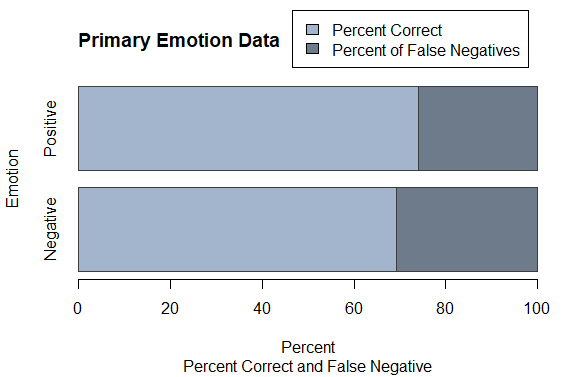
\includegraphics[width = 3.5in]{BarPlotPrimaryResults.png}
%	\caption{Barplot of Results of Primary Emotion Data, Positive and Negative Categories}
%	\label{bpprimem}
%\end{figure}

%\begin{subfigure}[]{6cm} \centering \resizebox{\linewidth}{!}{% This file was created by matplotlib2tikz v0.6.18.
\begin{tikzpicture}

\begin{axis}[
axis background/.style={fill=white!89.80392156862746!black},
axis line style={white},
height=6cm,
tick align=outside,
tick pos=left,
title={Sentiment Distribution of Chick-fil-A Twitter Comments},
width=9cm,
x grid style={white},
xlabel={Positive Sentiment Score},
xmajorgrids,
xmin=0, xmax=1,
xtick={0,0.2,0.4,0.6,0.8,1},
xticklabels={0.0,0.2,0.4,0.6,0.8,1.0},
y grid style={white},
ylabel={Percent of Scored Comments},
ymajorgrids,
ymin=0, ymax=7
]
\draw[fill=red,draw opacity=0] (axis cs:0.0219790190458298,0) rectangle (axis cs:0.0463351532816887,0.948521150382389);
\draw[fill=red,draw opacity=0] (axis cs:0.0463351532816887,0) rectangle (axis cs:0.0706912875175476,1.49053335030431);
\draw[fill=red,draw opacity=0] (axis cs:0.0706912875175476,0) rectangle (axis cs:0.0950474217534065,0.813018191075078);
\draw[fill=red,draw opacity=0] (axis cs:0.0950474292039871,0) rectangle (axis cs:0.119403563439846,0.677515159229232);
\draw[fill=red,draw opacity=0] (axis cs:0.119403563439846,0) rectangle (axis cs:0.143759697675705,1.62603588474317);
\draw[fill=red,draw opacity=0] (axis cs:0.143759697675705,0) rectangle (axis cs:0.168115824460983,0.271006146592908);
\draw[fill=red,draw opacity=0] (axis cs:0.168115824460983,0) rectangle (axis cs:0.192471966147423,1.21952691355738);
\draw[fill=red,draw opacity=0] (axis cs:0.192471966147423,0) rectangle (axis cs:0.216828092932701,0.813018439778725);
\draw[fill=red,draw opacity=0] (axis cs:0.216828107833862,0) rectangle (axis cs:0.241184249520302,0.813017942371583);
\draw[fill=red,draw opacity=0] (axis cs:0.241184234619141,0) rectangle (axis cs:0.265540361404419,0.94852151307518);
\draw[fill=red,draw opacity=0] (axis cs:0.265540361404419,0) rectangle (axis cs:0.289896488189697,0.813018439778725);
\draw[fill=red,draw opacity=0] (axis cs:0.289896488189697,0) rectangle (axis cs:0.314252644777298,1.35502907494175);
\draw[fill=red,draw opacity=0] (axis cs:0.314252644777298,0) rectangle (axis cs:0.338608771562576,0.271006146592908);
\draw[fill=red,draw opacity=0] (axis cs:0.338608771562576,0) rectangle (axis cs:0.362964898347855,0.542012293185817);
\draw[fill=red,draw opacity=0] (axis cs:0.362964898347855,0) rectangle (axis cs:0.387321025133133,0.813018439778725);
\draw[fill=red,draw opacity=0] (axis cs:0.387321054935455,0) rectangle (axis cs:0.411677211523056,0.27100581498835);
\draw[fill=red,draw opacity=0] (axis cs:0.411677181720734,0) rectangle (axis cs:0.436033308506012,1.08402458637163);
\draw[fill=red,draw opacity=0] (axis cs:0.436033308506012,0) rectangle (axis cs:0.46038943529129,0.542012293185817);
\draw[fill=red,draw opacity=0] (axis cs:0.46038943529129,0) rectangle (axis cs:0.484745562076569,0.406509219889363);
\draw[fill=red,draw opacity=0] (axis cs:0.484745562076569,0) rectangle (axis cs:0.509101688861847,0.677515366482271);
\draw[fill=red,draw opacity=0] (axis cs:0.509101688861847,0) rectangle (axis cs:0.533457815647125,0);
\draw[fill=red,draw opacity=0] (axis cs:0.53345787525177,0) rectangle (axis cs:0.557814061641693,0.677513708461508);
\draw[fill=red,draw opacity=0] (axis cs:0.557814002037048,0) rectangle (axis cs:0.582170128822327,1.08402458637163);
\draw[fill=red,draw opacity=0] (axis cs:0.582170128822327,0) rectangle (axis cs:0.606526255607605,0.135503073296454);
\draw[fill=red,draw opacity=0] (axis cs:0.606526255607605,0) rectangle (axis cs:0.630882382392883,0.271006146592908);
\draw[fill=red,draw opacity=0] (axis cs:0.630882382392883,0) rectangle (axis cs:0.655238509178162,0.271006146592908);
\draw[fill=red,draw opacity=0] (axis cs:0.655238509178162,0) rectangle (axis cs:0.67959463596344,0.813018439778725);
\draw[fill=red,draw opacity=0] (axis cs:0.67959463596344,0) rectangle (axis cs:0.703950762748718,0.813018439778725);
\draw[fill=red,draw opacity=0] (axis cs:0.703950762748718,0) rectangle (axis cs:0.728306949138641,0.542010966769206);
\draw[fill=red,draw opacity=0] (axis cs:0.728306949138641,0) rectangle (axis cs:0.75266307592392,0.542012293185817);
\draw[fill=red,draw opacity=0] (axis cs:0.75266307592392,0) rectangle (axis cs:0.777019202709198,0.813018439778725);
\draw[fill=red,draw opacity=0] (axis cs:0.777019202709198,0) rectangle (axis cs:0.801375329494476,0.677515366482271);
\draw[fill=red,draw opacity=0] (axis cs:0.801375329494476,0) rectangle (axis cs:0.825731456279755,1.08402458637163);
\draw[fill=red,draw opacity=0] (axis cs:0.825731456279755,0) rectangle (axis cs:0.850087583065033,1.7615399528539);
\draw[fill=red,draw opacity=0] (axis cs:0.850087583065033,0) rectangle (axis cs:0.874443709850311,1.21952765966809);
\draw[fill=red,draw opacity=0] (axis cs:0.874443709850311,0) rectangle (axis cs:0.89879983663559,1.490533806261);
\draw[fill=red,draw opacity=0] (axis cs:0.898799896240234,0) rectangle (axis cs:0.923156082630157,1.62603290030762);
\draw[fill=red,draw opacity=0] (axis cs:0.923156023025513,0) rectangle (axis cs:0.947512149810791,2.57455839263263);
\draw[fill=red,draw opacity=0] (axis cs:0.947512149810791,0) rectangle (axis cs:0.971868276596069,3.2520737591149);
\draw[fill=red,draw opacity=0] (axis cs:0.971868276596069,0) rectangle (axis cs:0.996224403381348,5.01361371196881);
\path [draw=white, fill opacity=0] (axis cs:0,0)
--(axis cs:0,7);

\path [draw=white, fill opacity=0] (axis cs:1,0)
--(axis cs:1,7);

\path [draw=white, fill opacity=0] (axis cs:0,0)
--(axis cs:1,0);

\path [draw=white, fill opacity=0] (axis cs:0,1)
--(axis cs:1,1);

\end{axis}
\label{chickt}
\end{tikzpicture} }  \caption{} \label{fig:chicktt} \end{subfigure
		
\begin{figure}[]
	\hfill
	\vspace*{-1in}
	\centering
	\begin{adjustwidth}{-.75in}{-.75in}
		
 \begin{subfigure}{3in}
 	\centering
 	\caption{Primary Emotion Accuracy}
	\resizebox{3in}{!}{% Created by tikzDevice version 0.12 on 2018-12-01 10:49:27
% !TEX encoding = UTF-8 Unicode

\begin{tikzpicture}[x=1pt,y=1pt]
\definecolor{fillColor}{RGB}{255,255,255}
\path[use as bounding box,fill=fillColor,fill opacity=0.00] (0,0) rectangle (361.35,361.35);
\begin{scope}
\path[clip] (  0.00,  0.00) rectangle (361.35,361.35);
\definecolor{drawColor}{gray}{0.24}
\definecolor{fillColor}{RGB}{162,181,205}

\path[draw=drawColor,line width= 0.4pt,line join=round,line cap=round,fill=fillColor] ( 49.20, 70.49) rectangle (248.09,176.11);
\definecolor{fillColor}{RGB}{110,123,139}

\path[draw=drawColor,line width= 0.4pt,line join=round,line cap=round,fill=fillColor] (248.09, 70.49) rectangle (336.12,176.11);
\definecolor{fillColor}{RGB}{162,181,205}

\path[draw=drawColor,line width= 0.4pt,line join=round,line cap=round,fill=fillColor] ( 49.20,197.24) rectangle (261.74,302.86);
\definecolor{fillColor}{RGB}{110,123,139}

\path[draw=drawColor,line width= 0.4pt,line join=round,line cap=round,fill=fillColor] (261.74,197.24) rectangle (336.12,302.86);
\end{scope}
\begin{scope}
\path[clip] (  0.00,  0.00) rectangle (361.35,361.35);
\definecolor{drawColor}{RGB}{0,0,0}

\node[text=drawColor,rotate= 90.00,anchor=base,inner sep=0pt, outer sep=0pt, scale=  1.00] at ( 34.80,123.30) {Negative};

\node[text=drawColor,rotate= 90.00,anchor=base,inner sep=0pt, outer sep=0pt, scale=  1.00] at ( 34.80,250.05) {Positive};
\end{scope}
\begin{scope}
\path[clip] (  0.00,  0.00) rectangle (361.35,361.35);
\definecolor{drawColor}{RGB}{0,0,0}

\path[draw=drawColor,line width= 0.4pt,line join=round,line cap=round] (184.39,345.10) rectangle (328.92,309.10);
\definecolor{fillColor}{RGB}{162,181,205}

\path[draw=drawColor,line width= 0.4pt,line join=round,line cap=round,fill=fillColor] (193.39,336.10) rectangle (200.59,330.10);
\definecolor{fillColor}{RGB}{110,123,139}

\path[draw=drawColor,line width= 0.4pt,line join=round,line cap=round,fill=fillColor] (193.39,324.10) rectangle (200.59,318.10);

\node[text=drawColor,anchor=base west,inner sep=0pt, outer sep=0pt, scale=  1.00] at (209.59,329.66) {Percent Correct};

\node[text=drawColor,anchor=base west,inner sep=0pt, outer sep=0pt, scale=  1.00] at (209.59,317.66) {Percent of False Negatives};

\node[text=drawColor,anchor=base west,inner sep=0pt, outer sep=0pt, scale=  1.20] at ( 49.20,332.61) {\bfseries Results of Primary Emotion Data};

\node[text=drawColor,anchor=base,inner sep=0pt, outer sep=0pt, scale=  1.00] at (192.68,  3.60) {Percent Correct and False Negative};

\node[text=drawColor,anchor=base,inner sep=0pt, outer sep=0pt, scale=  1.00] at (192.68, 15.60) {Percent};

\node[text=drawColor,rotate= 90.00,anchor=base,inner sep=0pt, outer sep=0pt, scale=  1.00] at ( 10.80,186.67) {Emotion};
\end{scope}
\begin{scope}
\path[clip] (  0.00,  0.00) rectangle (361.35,361.35);
\definecolor{drawColor}{RGB}{0,0,0}

\path[draw=drawColor,line width= 0.4pt,line join=round,line cap=round] ( 49.20, 61.20) -- (336.15, 61.20);

\path[draw=drawColor,line width= 0.4pt,line join=round,line cap=round] ( 49.20, 61.20) -- ( 49.20, 55.20);

\path[draw=drawColor,line width= 0.4pt,line join=round,line cap=round] (106.59, 61.20) -- (106.59, 55.20);

\path[draw=drawColor,line width= 0.4pt,line join=round,line cap=round] (163.98, 61.20) -- (163.98, 55.20);

\path[draw=drawColor,line width= 0.4pt,line join=round,line cap=round] (221.37, 61.20) -- (221.37, 55.20);

\path[draw=drawColor,line width= 0.4pt,line join=round,line cap=round] (278.76, 61.20) -- (278.76, 55.20);

\path[draw=drawColor,line width= 0.4pt,line join=round,line cap=round] (336.15, 61.20) -- (336.15, 55.20);

\node[text=drawColor,anchor=base,inner sep=0pt, outer sep=0pt, scale=  1.00] at ( 49.20, 39.60) {0};

\node[text=drawColor,anchor=base,inner sep=0pt, outer sep=0pt, scale=  1.00] at (106.59, 39.60) {20};

\node[text=drawColor,anchor=base,inner sep=0pt, outer sep=0pt, scale=  1.00] at (163.98, 39.60) {40};

\node[text=drawColor,anchor=base,inner sep=0pt, outer sep=0pt, scale=  1.00] at (221.37, 39.60) {60};

\node[text=drawColor,anchor=base,inner sep=0pt, outer sep=0pt, scale=  1.00] at (278.76, 39.60) {80};

\node[text=drawColor,anchor=base,inner sep=0pt, outer sep=0pt, scale=  1.00] at (336.15, 39.60) {100};
\end{scope}
\end{tikzpicture}
}
	\label{primemresult}
\end{subfigure}
\hfill
\begin{subfigure}{3in}
	\centering
	\caption{Labeled Twitter Data Accuracy}
	\resizebox{3in}{!}{% Created by tikzDevice version 0.12 on 2018-12-01 10:48:48
% !TEX encoding = UTF-8 Unicode
\begin{tikzpicture}[x=1pt,y=1pt]
\definecolor{fillColor}{RGB}{255,255,255}
\path[use as bounding box,fill=fillColor,fill opacity=0.00] (0,0) rectangle (361.35,361.35);
\begin{scope}
\path[clip] (  0.00,  0.00) rectangle (361.35,361.35);
\definecolor{drawColor}{gray}{0.37}
\definecolor{fillColor}{RGB}{124,205,124}

\path[draw=drawColor,line width= 0.4pt,line join=round,line cap=round,fill=fillColor] ( 49.20, 70.49) rectangle (309.64,176.11);
\definecolor{fillColor}{RGB}{84,139,84}

\path[draw=drawColor,line width= 0.4pt,line join=round,line cap=round,fill=fillColor] (309.64, 70.49) rectangle (336.12,176.11);
\definecolor{fillColor}{RGB}{124,205,124}

\path[draw=drawColor,line width= 0.4pt,line join=round,line cap=round,fill=fillColor] ( 49.20,197.24) rectangle (269.00,302.86);
\definecolor{fillColor}{RGB}{84,139,84}

\path[draw=drawColor,line width= 0.4pt,line join=round,line cap=round,fill=fillColor] (269.00,197.24) rectangle (336.12,302.86);
\end{scope}
\begin{scope}
\path[clip] (  0.00,  0.00) rectangle (361.35,361.35);
\definecolor{drawColor}{RGB}{0,0,0}

\node[text=drawColor,rotate= 90.00,anchor=base,inner sep=0pt, outer sep=0pt, scale=  1.00] at ( 34.80,123.30) {Negative};

\node[text=drawColor,rotate= 90.00,anchor=base,inner sep=0pt, outer sep=0pt, scale=  1.00] at ( 34.80,250.05) {Positive};
\end{scope}
\begin{scope}
\path[clip] (  0.00,  0.00) rectangle (361.35,361.35);
\definecolor{drawColor}{RGB}{0,0,0}

\path[draw=drawColor,line width= 0.4pt,line join=round,line cap=round] (184.39,345.10) rectangle (328.92,309.10);
\definecolor{fillColor}{RGB}{124,205,124}

\path[draw=drawColor,line width= 0.4pt,line join=round,line cap=round,fill=fillColor] (193.39,336.10) rectangle (200.59,330.10);
\definecolor{fillColor}{RGB}{84,139,84}

\path[draw=drawColor,line width= 0.4pt,line join=round,line cap=round,fill=fillColor] (193.39,324.10) rectangle (200.59,318.10);

\node[text=drawColor,anchor=base west,inner sep=0pt, outer sep=0pt, scale=  1.00] at (209.59,329.66) {Percent Correct};

\node[text=drawColor,anchor=base west,inner sep=0pt, outer sep=0pt, scale=  1.00] at (209.59,317.66) {Percent of False Negatives};

\node[text=drawColor,anchor=base west,inner sep=0pt, outer sep=0pt, scale=  1.20] at ( 49.20,332.61) {\bfseries Results of Twitter Data};

\node[text=drawColor,anchor=base,inner sep=0pt, outer sep=0pt, scale=  1.00] at (192.68,  3.60) {Percent Correct and False Negative};

\node[text=drawColor,anchor=base,inner sep=0pt, outer sep=0pt, scale=  1.00] at (192.68, 15.60) {Percent};

\node[text=drawColor,rotate= 90.00,anchor=base,inner sep=0pt, outer sep=0pt, scale=  1.00] at ( 10.80,186.67) {Emotion};
\end{scope}
\begin{scope}
\path[clip] (  0.00,  0.00) rectangle (361.35,361.35);
\definecolor{drawColor}{RGB}{0,0,0}

\path[draw=drawColor,line width= 0.4pt,line join=round,line cap=round] ( 49.20, 61.20) -- (336.15, 61.20);

\path[draw=drawColor,line width= 0.4pt,line join=round,line cap=round] ( 49.20, 61.20) -- ( 49.20, 55.20);

\path[draw=drawColor,line width= 0.4pt,line join=round,line cap=round] (106.59, 61.20) -- (106.59, 55.20);

\path[draw=drawColor,line width= 0.4pt,line join=round,line cap=round] (163.98, 61.20) -- (163.98, 55.20);

\path[draw=drawColor,line width= 0.4pt,line join=round,line cap=round] (221.37, 61.20) -- (221.37, 55.20);

\path[draw=drawColor,line width= 0.4pt,line join=round,line cap=round] (278.76, 61.20) -- (278.76, 55.20);

\path[draw=drawColor,line width= 0.4pt,line join=round,line cap=round] (336.15, 61.20) -- (336.15, 55.20);

\node[text=drawColor,anchor=base,inner sep=0pt, outer sep=0pt, scale=  1.00] at ( 49.20, 39.60) {0};

\node[text=drawColor,anchor=base,inner sep=0pt, outer sep=0pt, scale=  1.00] at (106.59, 39.60) {20};

\node[text=drawColor,anchor=base,inner sep=0pt, outer sep=0pt, scale=  1.00] at (163.98, 39.60) {40};

\node[text=drawColor,anchor=base,inner sep=0pt, outer sep=0pt, scale=  1.00] at (221.37, 39.60) {60};

\node[text=drawColor,anchor=base,inner sep=0pt, outer sep=0pt, scale=  1.00] at (278.76, 39.60) {80};

\node[text=drawColor,anchor=base,inner sep=0pt, outer sep=0pt, scale=  1.00] at (336.15, 39.60) {100};
\end{scope}
\end{tikzpicture}
}
	\label{lbtwitresult}
\end{subfigure}
\hfill
\end{adjustwidth}
\caption{Testing Accuracy Of Training Data Sets}\label{duo_chart}
\end{figure}
\subsection{Labeled Twitter Data Results}

The sampled Twitter data was collected by Figure Eight \cite{LabeledTwitter} and consists of about $40,000$ tweets, assigned emotion, and user identification. There are some cases of multiple tweets from the same person. The emotion categories are empty, sadness, enthusiasm, neutral, worry, love, fun, hate, happiness, surprise, and boredom. The twitter data was split into positive and negative categories, where the positive category contains the emotion groups enthusiasm, love, and happiness, and the negative category contains the emotion groups sadness and hate. The other emotions are ignored since they do not fall into completely positive or negative categories. 

 \begin{center}
	\captionof{table}{Labeled Twitter Data}
	\begin{tabular}{ |c|c| } 
		\hline
		Emotion & Tweet \\
		\hline \hline
		happiness & mmm much better day... so far! it's still quite\\
		 & early. last day of uds \\
		\hline
		worry &  sucks not being able to take days off of work or \\
		& have the money to take the trip  so sad \\
		\hline
		hate & dammit! hulu desktop has totally screwed up my ability \\
		& to talk to a particular port on one of our dev servers. \\
		& so i can't watch and code  \\ 
		\hline
		love & @RobertF3 correct! I ADORE him. I just plucked him up \\ 
		& and put him under my arm cuz he was cryin.  All better now! \\ & Hahaha \\
		\hline
	\end{tabular}
	\label{McdonaldsServiceFailureTable}
\end{center}

The training set contained $90$ percent of the data and had an accuracy of $82.3$ percent. The testing set contained the remaining $10$ percent of the data and had an accuracy of $83.3$ percent. The testing accuracy was actually higher than the training accuracy and both values were very close which indicates the method was not over-fitting to the training data. We note that the testing set of the Labeled Twitter data contained a higher percentage of the Labeled Twitter data compared to the testing set of the Primary Emotion data since the Labeled Twitter data is a much bigger data set, and $10$ percent of the data was more than an adequate size for testing set. 

Figure \ref{lbtwitresult} gives a barplot containing the results of the testing accuracy for the Twitter data; again there is a bar for both the negative and positive results. The light green shows the percent of correct predictions for each group. The dark green bar shows the percent of false negatives for each group. In other words, the percent of sentences that should have been predicted to be positive in the positive bar, or negative in the negative bar. 
 barplot we can see that the model is doing a great job of predicting negative sentiment in the Twitter data but not quiet as well when predicting the positive sentiment. However the percent of correctly predicted positive sentiment for the Twitter data is about the same as the percent of correctly predicted positive sentiment in the Primary Emotion data. Most companies want to know which areas they are succeeding in, but they also need to know in which areas they can improve. If the model can accurately find negative sentiment in a tweet or a comment, we can then make recommendations based on that output about which reviews the company should be taking more seriously. 

%\begin{figure}[h!]
%	\centering
%	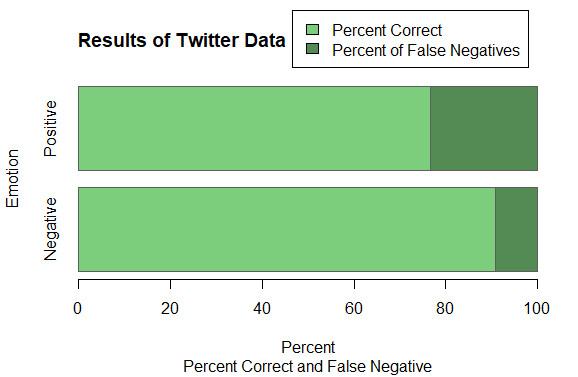
\includegraphics[width = 3.5in]{BarPlotTwitterResults.png}
%	\caption{Barplot of Results of Twitter Data, Positive and Negative Categories}
%\end{figure}


\subsection{Unlabeled Raw Twitter Data Results}

\begin{figure}[h!]

\begin{adjustwidth}{-1in}{-1in}
\begin{subfigure}[]{6cm} \centering \resizebox{\linewidth}{!}{% This file was created by matplotlib2tikz v0.6.18.
\begin{tikzpicture}

\begin{axis}[
axis background/.style={fill=white!89.80392156862746!black},
axis line style={white},
height=6cm,
tick align=outside,
tick pos=left,
title={Sentiment Distribution of Chick-fil-A Twitter Comments},
width=9cm,
x grid style={white},
xlabel={Positive Sentiment Score},
xmajorgrids,
xmin=0, xmax=1,
xtick={0,0.2,0.4,0.6,0.8,1},
xticklabels={0.0,0.2,0.4,0.6,0.8,1.0},
y grid style={white},
ylabel={Percent of Scored Comments},
ymajorgrids,
ymin=0, ymax=7
]
\draw[fill=red,draw opacity=0] (axis cs:0.0219790190458298,0) rectangle (axis cs:0.0463351532816887,0.948521150382389);
\draw[fill=red,draw opacity=0] (axis cs:0.0463351532816887,0) rectangle (axis cs:0.0706912875175476,1.49053335030431);
\draw[fill=red,draw opacity=0] (axis cs:0.0706912875175476,0) rectangle (axis cs:0.0950474217534065,0.813018191075078);
\draw[fill=red,draw opacity=0] (axis cs:0.0950474292039871,0) rectangle (axis cs:0.119403563439846,0.677515159229232);
\draw[fill=red,draw opacity=0] (axis cs:0.119403563439846,0) rectangle (axis cs:0.143759697675705,1.62603588474317);
\draw[fill=red,draw opacity=0] (axis cs:0.143759697675705,0) rectangle (axis cs:0.168115824460983,0.271006146592908);
\draw[fill=red,draw opacity=0] (axis cs:0.168115824460983,0) rectangle (axis cs:0.192471966147423,1.21952691355738);
\draw[fill=red,draw opacity=0] (axis cs:0.192471966147423,0) rectangle (axis cs:0.216828092932701,0.813018439778725);
\draw[fill=red,draw opacity=0] (axis cs:0.216828107833862,0) rectangle (axis cs:0.241184249520302,0.813017942371583);
\draw[fill=red,draw opacity=0] (axis cs:0.241184234619141,0) rectangle (axis cs:0.265540361404419,0.94852151307518);
\draw[fill=red,draw opacity=0] (axis cs:0.265540361404419,0) rectangle (axis cs:0.289896488189697,0.813018439778725);
\draw[fill=red,draw opacity=0] (axis cs:0.289896488189697,0) rectangle (axis cs:0.314252644777298,1.35502907494175);
\draw[fill=red,draw opacity=0] (axis cs:0.314252644777298,0) rectangle (axis cs:0.338608771562576,0.271006146592908);
\draw[fill=red,draw opacity=0] (axis cs:0.338608771562576,0) rectangle (axis cs:0.362964898347855,0.542012293185817);
\draw[fill=red,draw opacity=0] (axis cs:0.362964898347855,0) rectangle (axis cs:0.387321025133133,0.813018439778725);
\draw[fill=red,draw opacity=0] (axis cs:0.387321054935455,0) rectangle (axis cs:0.411677211523056,0.27100581498835);
\draw[fill=red,draw opacity=0] (axis cs:0.411677181720734,0) rectangle (axis cs:0.436033308506012,1.08402458637163);
\draw[fill=red,draw opacity=0] (axis cs:0.436033308506012,0) rectangle (axis cs:0.46038943529129,0.542012293185817);
\draw[fill=red,draw opacity=0] (axis cs:0.46038943529129,0) rectangle (axis cs:0.484745562076569,0.406509219889363);
\draw[fill=red,draw opacity=0] (axis cs:0.484745562076569,0) rectangle (axis cs:0.509101688861847,0.677515366482271);
\draw[fill=red,draw opacity=0] (axis cs:0.509101688861847,0) rectangle (axis cs:0.533457815647125,0);
\draw[fill=red,draw opacity=0] (axis cs:0.53345787525177,0) rectangle (axis cs:0.557814061641693,0.677513708461508);
\draw[fill=red,draw opacity=0] (axis cs:0.557814002037048,0) rectangle (axis cs:0.582170128822327,1.08402458637163);
\draw[fill=red,draw opacity=0] (axis cs:0.582170128822327,0) rectangle (axis cs:0.606526255607605,0.135503073296454);
\draw[fill=red,draw opacity=0] (axis cs:0.606526255607605,0) rectangle (axis cs:0.630882382392883,0.271006146592908);
\draw[fill=red,draw opacity=0] (axis cs:0.630882382392883,0) rectangle (axis cs:0.655238509178162,0.271006146592908);
\draw[fill=red,draw opacity=0] (axis cs:0.655238509178162,0) rectangle (axis cs:0.67959463596344,0.813018439778725);
\draw[fill=red,draw opacity=0] (axis cs:0.67959463596344,0) rectangle (axis cs:0.703950762748718,0.813018439778725);
\draw[fill=red,draw opacity=0] (axis cs:0.703950762748718,0) rectangle (axis cs:0.728306949138641,0.542010966769206);
\draw[fill=red,draw opacity=0] (axis cs:0.728306949138641,0) rectangle (axis cs:0.75266307592392,0.542012293185817);
\draw[fill=red,draw opacity=0] (axis cs:0.75266307592392,0) rectangle (axis cs:0.777019202709198,0.813018439778725);
\draw[fill=red,draw opacity=0] (axis cs:0.777019202709198,0) rectangle (axis cs:0.801375329494476,0.677515366482271);
\draw[fill=red,draw opacity=0] (axis cs:0.801375329494476,0) rectangle (axis cs:0.825731456279755,1.08402458637163);
\draw[fill=red,draw opacity=0] (axis cs:0.825731456279755,0) rectangle (axis cs:0.850087583065033,1.7615399528539);
\draw[fill=red,draw opacity=0] (axis cs:0.850087583065033,0) rectangle (axis cs:0.874443709850311,1.21952765966809);
\draw[fill=red,draw opacity=0] (axis cs:0.874443709850311,0) rectangle (axis cs:0.89879983663559,1.490533806261);
\draw[fill=red,draw opacity=0] (axis cs:0.898799896240234,0) rectangle (axis cs:0.923156082630157,1.62603290030762);
\draw[fill=red,draw opacity=0] (axis cs:0.923156023025513,0) rectangle (axis cs:0.947512149810791,2.57455839263263);
\draw[fill=red,draw opacity=0] (axis cs:0.947512149810791,0) rectangle (axis cs:0.971868276596069,3.2520737591149);
\draw[fill=red,draw opacity=0] (axis cs:0.971868276596069,0) rectangle (axis cs:0.996224403381348,5.01361371196881);
\path [draw=white, fill opacity=0] (axis cs:0,0)
--(axis cs:0,7);

\path [draw=white, fill opacity=0] (axis cs:1,0)
--(axis cs:1,7);

\path [draw=white, fill opacity=0] (axis cs:0,0)
--(axis cs:1,0);

\path [draw=white, fill opacity=0] (axis cs:0,1)
--(axis cs:1,1);

\end{axis}
\label{chickt}
\end{tikzpicture} }  \label{fig:subfig8} \end{subfigure} \begin{subfigure}[]{6cm} \centering \resizebox{\linewidth}{!}{ % This file was created by matplotlib2tikz v0.6.18.
\begin{tikzpicture}

\definecolor{color0}{rgb}{0.580392156862745,0,0.827450980392157}

\begin{axis}[
axis background/.style={fill=white!89.80392156862746!black},
axis line style={white},
height=6cm,
tick align=outside,
tick pos=left,
title={Sentiment Distribution of Taco Bell Twitter Comments},
width=9cm,
x grid style={white},
xlabel={Positive Sentiment Score},
xmajorgrids,
xmin=0, xmax=1,
xtick={0,0.2,0.4,0.6,0.8,1},
xticklabels={0.0,0.2,0.4,0.6,0.8,1.0},
y grid style={white},
ylabel={Percent of Scored Comments},
ymajorgrids,
ymin=0, ymax=7
]
\draw[fill=color0,draw opacity=0] (axis cs:0.0242587197571993,0) rectangle (axis cs:0.048572301864624,0.376704460881885);
\draw[fill=color0,draw opacity=0] (axis cs:0.048572301864624,0) rectangle (axis cs:0.0728858858346939,0.616425386995312);
\draw[fill=color0,draw opacity=0] (axis cs:0.0728858858346939,0) rectangle (axis cs:0.0971994623541832,0.513687979909073);
\draw[fill=color0,draw opacity=0] (axis cs:0.0971994623541832,0) rectangle (axis cs:0.121513046324253,0.924638080492968);
\draw[fill=color0,draw opacity=0] (axis cs:0.121513053774834,0) rectangle (axis cs:0.145826637744904,0.513687979909073);
\draw[fill=color0,draw opacity=0] (axis cs:0.145826637744904,0) rectangle (axis cs:0.170140221714973,0.684917096661458);
\draw[fill=color0,draw opacity=0] (axis cs:0.170140206813812,0) rectangle (axis cs:0.194453790783882,0.205475128998437);
\draw[fill=color0,draw opacity=0] (axis cs:0.194453805685043,0) rectangle (axis cs:0.218767389655113,0.71916295149453);
\draw[fill=color0,draw opacity=0] (axis cs:0.218767374753952,0) rectangle (axis cs:0.243080958724022,0.513687822496093);
\draw[fill=color0,draw opacity=0] (axis cs:0.243080973625183,0) rectangle (axis cs:0.267394542694092,0.890392225659895);
\draw[fill=color0,draw opacity=0] (axis cs:0.267394542694092,0) rectangle (axis cs:0.291708111763,0.616425764786579);
\draw[fill=color0,draw opacity=0] (axis cs:0.291708111763,0) rectangle (axis cs:0.316021710634232,0.239720836912864);
\draw[fill=color0,draw opacity=0] (axis cs:0.316021710634232,0) rectangle (axis cs:0.34033527970314,0.753409268072485);
\draw[fill=color0,draw opacity=0] (axis cs:0.34033527970314,0) rectangle (axis cs:0.364648848772049,0.479442261500672);
\draw[fill=color0,draw opacity=0] (axis cs:0.364648878574371,0) rectangle (axis cs:0.388962477445602,0.308212504602254);
\draw[fill=color0,draw opacity=0] (axis cs:0.38896244764328,0) rectangle (axis cs:0.413276016712189,0.650671640608055);
\draw[fill=color0,draw opacity=0] (axis cs:0.413276016712189,0) rectangle (axis cs:0.43758961558342,0.582179175359813);
\draw[fill=color0,draw opacity=0] (axis cs:0.43758961558342,0) rectangle (axis cs:0.461903184652328,0.684917516429532);
\draw[fill=color0,draw opacity=0] (axis cs:0.461903184652328,0) rectangle (axis cs:0.486216753721237,0.856146895536915);
\draw[fill=color0,draw opacity=0] (axis cs:0.48621678352356,0) rectangle (axis cs:0.510530352592468,1.02737501534085);
\draw[fill=color0,draw opacity=0] (axis cs:0.510530352592468,0) rectangle (axis cs:0.534843921661377,0.650671640608055);
\draw[fill=color0,draw opacity=0] (axis cs:0.534843921661377,0) rectangle (axis cs:0.559157490730286,0.342458758214766);
\draw[fill=color0,draw opacity=0] (axis cs:0.559157490730286,0) rectangle (axis cs:0.583471119403839,3.15061285185748);
\draw[fill=color0,draw opacity=0] (axis cs:0.583471119403839,0) rectangle (axis cs:0.607784688472748,0.479442261500672);
\draw[fill=color0,draw opacity=0] (axis cs:0.607784688472748,0) rectangle (axis cs:0.632098257541656,0.616425764786579);
\draw[fill=color0,draw opacity=0] (axis cs:0.632098257541656,0) rectangle (axis cs:0.656411826610565,1.47257266032349);
\draw[fill=color0,draw opacity=0] (axis cs:0.656411826610565,0) rectangle (axis cs:0.680725395679474,0.958884523001344);
\draw[fill=color0,draw opacity=0] (axis cs:0.680725336074829,0) rectangle (axis cs:0.705038964748383,0.821899004832387);
\draw[fill=color0,draw opacity=0] (axis cs:0.705039024353027,0) rectangle (axis cs:0.729352593421936,1.13011390210873);
\draw[fill=color0,draw opacity=0] (axis cs:0.729352593421936,0) rectangle (axis cs:0.753666162490845,0.719163392251008);
\draw[fill=color0,draw opacity=0] (axis cs:0.753666162490845,0) rectangle (axis cs:0.777979731559753,1.54106441196645);
\draw[fill=color0,draw opacity=0] (axis cs:0.777979731559753,0) rectangle (axis cs:0.802293300628662,0.958884523001344);
\draw[fill=color0,draw opacity=0] (axis cs:0.802293300628662,0) rectangle (axis cs:0.826606929302216,0.890390588568419);
\draw[fill=color0,draw opacity=0] (axis cs:0.826606929302216,0) rectangle (axis cs:0.850920498371124,2.22598192839598);
\draw[fill=color0,draw opacity=0] (axis cs:0.850920498371124,0) rectangle (axis cs:0.875234067440033,1.1643597779302);
\draw[fill=color0,draw opacity=0] (axis cs:0.875234067440033,0) rectangle (axis cs:0.899547636508942,1.23285152957316);
\draw[fill=color0,draw opacity=0] (axis cs:0.899547636508942,0) rectangle (axis cs:0.92386120557785,2.02050667346712);
\draw[fill=color0,draw opacity=0] (axis cs:0.923861145973206,0) rectangle (axis cs:0.948174774646759,2.15748488768502);
\draw[fill=color0,draw opacity=0] (axis cs:0.948174834251404,0) rectangle (axis cs:0.972488403320312,1.50681853614497);
\draw[fill=color0,draw opacity=0] (axis cs:0.972488403320312,0) rectangle (axis cs:0.996801972389221,4.93140611829263);
\path [draw=white, fill opacity=0] (axis cs:0,0)
--(axis cs:0,7);

\path [draw=white, fill opacity=0] (axis cs:1,0)
--(axis cs:1,7);

\path [draw=white, fill opacity=0] (axis cs:0,0)
--(axis cs:1,0);

\path [draw=white, fill opacity=0] (axis cs:0,1)
--(axis cs:1,1);

\end{axis}
\label{tacot}
\end{tikzpicture}\hfill }  \label{fig:subfig9} \end{subfigure} \begin{subfigure}[]{6cm} \centering \resizebox{\linewidth}{!}{ 
% This file was created by matplotlib2tikz v0.6.18.
\begin{tikzpicture}

\definecolor{color0}{rgb}{0.250980392156863,0.87843137254902,0.815686274509804}

\begin{axis}[
axis background/.style={fill=white!89.80392156862746!black},
axis line style={white},
height=4cm,
tick align=outside,
tick pos=left,
title={Sentiment Distribution of Pal's},
width=6cm,
x grid style={white},
xlabel={Positive Sentiment Score},
xmajorgrids,
xmin=0, xmax=1,
xtick={0,0.2,0.4,0.6,0.8,1},
xticklabels={0.0,0.2,0.4,0.6,0.8,1.0},
y grid style={white},
ylabel={Percent},
ymajorgrids,
ymin=0, ymax=7
]
\draw[fill=color0,draw opacity=0] (axis cs:0.0140848532319069,0) rectangle (axis cs:0.0386082269251347,0.520562855930947);
\draw[fill=color0,draw opacity=0] (axis cs:0.0386082231998444,0) rectangle (axis cs:0.0631316006183624,0.983285394536234);
\draw[fill=color0,draw opacity=0] (axis cs:0.0631316006183624,0) rectangle (axis cs:0.0876549705862999,0.404882282784379);
\draw[fill=color0,draw opacity=0] (axis cs:0.0876549705862999,0) rectangle (axis cs:0.112178348004818,0.694083702471243);
\draw[fill=color0,draw opacity=0] (axis cs:0.112178340554237,0) rectangle (axis cs:0.136701703071594,0.925445217792865);
\draw[fill=color0,draw opacity=0] (axis cs:0.136701717972755,0) rectangle (axis cs:0.161225095391273,1.21464647932467);
\draw[fill=color0,draw opacity=0] (axis cs:0.161225095391273,0) rectangle (axis cs:0.185748472809792,0.867604628089053);
\draw[fill=color0,draw opacity=0] (axis cs:0.18574845790863,0) rectangle (axis cs:0.210271820425987,1.56168927949091);
\draw[fill=color0,draw opacity=0] (axis cs:0.210271835327148,0) rectangle (axis cs:0.234795212745667,0.925444936628323);
\draw[fill=color0,draw opacity=0] (axis cs:0.234795212745667,0) rectangle (axis cs:0.259318590164185,1.21464647932467);
\draw[fill=color0,draw opacity=0] (axis cs:0.259318590164185,0) rectangle (axis cs:0.283841967582703,1.27248678786394);
\draw[fill=color0,draw opacity=0] (axis cs:0.283841967582703,0) rectangle (axis cs:0.308365345001221,0.751924011010513);
\draw[fill=color0,draw opacity=0] (axis cs:0.308365345001221,0) rectangle (axis cs:0.332888722419739,0.404882159774892);
\draw[fill=color0,draw opacity=0] (axis cs:0.332888722419739,0) rectangle (axis cs:0.357412070035934,0.636244167135168);
\draw[fill=color0,draw opacity=0] (axis cs:0.357412070035934,0) rectangle (axis cs:0.381935447454453,1.04112555370686);
\draw[fill=color0,draw opacity=0] (axis cs:0.381935447454453,0) rectangle (axis cs:0.406458824872971,0.404882159774892);
\draw[fill=color0,draw opacity=0] (axis cs:0.406458824872971,0) rectangle (axis cs:0.430982202291489,1.33032709640321);
\draw[fill=color0,draw opacity=0] (axis cs:0.430982202291489,0) rectangle (axis cs:0.455505579710007,0.347041851235621);
\draw[fill=color0,draw opacity=0] (axis cs:0.455505579710007,0) rectangle (axis cs:0.480028957128525,0.404882159774892);
\draw[fill=color0,draw opacity=0] (axis cs:0.480028927326202,0) rectangle (axis cs:0.504552245140076,0.751924924796108);
\draw[fill=color0,draw opacity=0] (axis cs:0.50455230474472,0) rectangle (axis cs:0.529075682163239,0.11568061707854);
\draw[fill=color0,draw opacity=0] (axis cs:0.529075682163239,0) rectangle (axis cs:0.553599059581757,0.636243393931972);
\draw[fill=color0,draw opacity=0] (axis cs:0.553599059581757,0) rectangle (axis cs:0.578122437000275,2.19793172449227);
\draw[fill=color0,draw opacity=0] (axis cs:0.578122437000275,0) rectangle (axis cs:0.602645814418793,0.347041851235621);
\draw[fill=color0,draw opacity=0] (axis cs:0.602645814418793,0) rectangle (axis cs:0.627169191837311,0.751924011010513);
\draw[fill=color0,draw opacity=0] (axis cs:0.627169191837311,0) rectangle (axis cs:0.651692569255829,0.694083702471243);
\draw[fill=color0,draw opacity=0] (axis cs:0.651692569255829,0) rectangle (axis cs:0.676215946674347,0.751924011010513);
\draw[fill=color0,draw opacity=0] (axis cs:0.676215946674347,0) rectangle (axis cs:0.700739324092865,0.404882159774892);
\draw[fill=color0,draw opacity=0] (axis cs:0.700739324092865,0) rectangle (axis cs:0.725262701511383,2.25577203303154);
\draw[fill=color0,draw opacity=0] (axis cs:0.725262701511383,0) rectangle (axis cs:0.749786078929901,0.636243393931972);
\draw[fill=color0,draw opacity=0] (axis cs:0.749786078929901,0) rectangle (axis cs:0.774309456348419,0.694083702471243);
\draw[fill=color0,draw opacity=0] (axis cs:0.774309456348419,0) rectangle (axis cs:0.798832833766937,1.09896586224613);
\draw[fill=color0,draw opacity=0] (axis cs:0.798832893371582,0) rectangle (axis cs:0.823356211185455,0.925447185949444);
\draw[fill=color0,draw opacity=0] (axis cs:0.823356151580811,0) rectangle (axis cs:0.847879528999329,3.00769604404205);
\draw[fill=color0,draw opacity=0] (axis cs:0.847879528999329,0) rectangle (axis cs:0.872402906417847,0.694083702471243);
\draw[fill=color0,draw opacity=0] (axis cs:0.872402906417847,0) rectangle (axis cs:0.896926283836365,1.1568061707854);
\draw[fill=color0,draw opacity=0] (axis cs:0.896926283836365,0) rectangle (axis cs:0.921449661254883,0.925444936628323);
\draw[fill=color0,draw opacity=0] (axis cs:0.921449661254883,0) rectangle (axis cs:0.945973038673401,1.5616883305603);
\draw[fill=color0,draw opacity=0] (axis cs:0.945973038673401,0) rectangle (axis cs:0.970496416091919,1.27248678786394);
\draw[fill=color0,draw opacity=0] (axis cs:0.970496416091919,0) rectangle (axis cs:0.995019793510437,3.99098128920964);
\path [draw=white, fill opacity=0] (axis cs:0,0)
--(axis cs:0,7);

\path [draw=white, fill opacity=0] (axis cs:1,0)
--(axis cs:1,7);

\path [draw=white, fill opacity=0] (axis cs:0,0)
--(axis cs:1,0);

\path [draw=white, fill opacity=0] (axis cs:0,1)
--(axis cs:1,1);

\end{axis}

\end{tikzpicture} }  \label{fig:subfig10} \end{subfigure}  \label{fig:subfig1.a.4} 
\begin{subfigure}[]{6cm} \centering \resizebox{\linewidth}{!}{% This file was created by matplotlib2tikz v0.6.18.
\begin{tikzpicture}

\definecolor{color0}{rgb}{0.698039215686274,0.133333333333333,0.133333333333333}

\begin{axis}[
axis background/.style={fill=white!89.80392156862746!black},
axis line style={white},
height=4cm,
tick align=outside,
tick pos=left,
title={Sentiment Distribution of Chipotle Twitter Comments},
width=6cm,
x grid style={white},
xlabel={Positive Sentiment Score},
xmajorgrids,
xmin=0, xmax=1,
xtick={0,0.2,0.4,0.6,0.8,1},
xticklabels={0.0,0.2,0.4,0.6,0.8,1.0},
y grid style={white},
ylabel={Percent of Scored Comments},
ymajorgrids,
ymin=0, ymax=7
]
\draw[fill=color0,draw opacity=0] (axis cs:0.0257699713110924,0) rectangle (axis cs:0.0492510721087456,4.96853520312578);
\draw[fill=color0,draw opacity=0] (axis cs:0.0492510721087456,0) rectangle (axis cs:0.0727321654558182,4.96853638551765);
\draw[fill=color0,draw opacity=0] (axis cs:0.0727321654558182,0) rectangle (axis cs:0.0962132662534714,4.96853480899528);
\draw[fill=color0,draw opacity=0] (axis cs:0.0962132662534714,0) rectangle (axis cs:0.119694359600544,3.54895456108404);
\draw[fill=color0,draw opacity=0] (axis cs:0.119694352149963,0) rectangle (axis cs:0.143175452947617,0);
\draw[fill=color0,draw opacity=0] (axis cs:0.143175452947617,0) rectangle (axis cs:0.16665655374527,0.709790686999325);
\draw[fill=color0,draw opacity=0] (axis cs:0.16665655374527,0) rectangle (axis cs:0.190137654542923,1.41958137399865);
\draw[fill=color0,draw opacity=0] (axis cs:0.190137654542923,0) rectangle (axis cs:0.213618755340576,1.41958137399865);
\draw[fill=color0,draw opacity=0] (axis cs:0.213618755340576,0) rectangle (axis cs:0.237099841237068,2.83916454973773);
\draw[fill=color0,draw opacity=0] (axis cs:0.237099826335907,0) rectangle (axis cs:0.260580956935883,0);
\draw[fill=color0,draw opacity=0] (axis cs:0.260580956935883,0) rectangle (axis cs:0.284062027931213,3.54895793935056);
\draw[fill=color0,draw opacity=0] (axis cs:0.284062027931213,0) rectangle (axis cs:0.307543128728867,1.41958137399865);
\draw[fill=color0,draw opacity=0] (axis cs:0.307543098926544,0) rectangle (axis cs:0.331024199724197,2.12937206099798);
\draw[fill=color0,draw opacity=0] (axis cs:0.33102422952652,0) rectangle (axis cs:0.354505330324173,0);
\draw[fill=color0,draw opacity=0] (axis cs:0.354505300521851,0) rectangle (axis cs:0.377986401319504,0);
\draw[fill=color0,draw opacity=0] (axis cs:0.377986431121826,0) rectangle (axis cs:0.401467531919479,0);
\draw[fill=color0,draw opacity=0] (axis cs:0.401467502117157,0) rectangle (axis cs:0.42494860291481,0);
\draw[fill=color0,draw opacity=0] (axis cs:0.424948632717133,0) rectangle (axis cs:0.448429733514786,0);
\draw[fill=color0,draw opacity=0] (axis cs:0.448429703712463,0) rectangle (axis cs:0.471910804510117,0);
\draw[fill=color0,draw opacity=0] (axis cs:0.471910834312439,0) rectangle (axis cs:0.49539190530777,0);
\draw[fill=color0,draw opacity=0] (axis cs:0.49539190530777,0) rectangle (axis cs:0.518873035907745,0);
\draw[fill=color0,draw opacity=0] (axis cs:0.518872976303101,0) rectangle (axis cs:0.542354047298431,0);
\draw[fill=color0,draw opacity=0] (axis cs:0.542354106903076,0) rectangle (axis cs:0.565835237503052,0.709789786130826);
\draw[fill=color0,draw opacity=0] (axis cs:0.565835237503052,0) rectangle (axis cs:0.589316308498383,0);
\draw[fill=color0,draw opacity=0] (axis cs:0.589316248893738,0) rectangle (axis cs:0.612797319889069,0);
\draw[fill=color0,draw opacity=0] (axis cs:0.612797379493713,0) rectangle (axis cs:0.636278510093689,0);
\draw[fill=color0,draw opacity=0] (axis cs:0.636278510093689,0) rectangle (axis cs:0.65975958108902,0.709791587870111);
\draw[fill=color0,draw opacity=0] (axis cs:0.65975958108902,0) rectangle (axis cs:0.683240711688995,0);
\draw[fill=color0,draw opacity=0] (axis cs:0.683240652084351,0) rectangle (axis cs:0.706721723079681,2.83916635148044);
\draw[fill=color0,draw opacity=0] (axis cs:0.706721782684326,0) rectangle (axis cs:0.730202913284302,0);
\draw[fill=color0,draw opacity=0] (axis cs:0.730202913284302,0) rectangle (axis cs:0.753683984279633,0);
\draw[fill=color0,draw opacity=0] (axis cs:0.753683924674988,0) rectangle (axis cs:0.777164995670319,0.709791587870111);
\draw[fill=color0,draw opacity=0] (axis cs:0.777165055274963,0) rectangle (axis cs:0.800646185874939,0);
\draw[fill=color0,draw opacity=0] (axis cs:0.800646185874939,0) rectangle (axis cs:0.82412725687027,0.709791587870111);
\draw[fill=color0,draw opacity=0] (axis cs:0.82412725687027,0) rectangle (axis cs:0.847608387470245,1.41957957226165);
\draw[fill=color0,draw opacity=0] (axis cs:0.847608327865601,0) rectangle (axis cs:0.871089398860931,0.709791587870111);
\draw[fill=color0,draw opacity=0] (axis cs:0.871089458465576,0) rectangle (axis cs:0.894570589065552,1.41957957226165);
\draw[fill=color0,draw opacity=0] (axis cs:0.894570589065552,0) rectangle (axis cs:0.918051660060883,0);
\draw[fill=color0,draw opacity=0] (axis cs:0.918051660060883,0) rectangle (axis cs:0.941532790660858,0);
\draw[fill=color0,draw opacity=0] (axis cs:0.941532731056213,0) rectangle (axis cs:0.965013802051544,1.41958317574022);
\path [draw=white, fill opacity=0] (axis cs:0,0)
--(axis cs:0,7);

\path [draw=white, fill opacity=0] (axis cs:1,0)
--(axis cs:1,7);

\path [draw=white, fill opacity=0] (axis cs:0,0)
--(axis cs:1,0);

\path [draw=white, fill opacity=0] (axis cs:0,1)
--(axis cs:1,1);

\end{axis}

\end{tikzpicture} }  \label{fig:subfig8} \end{subfigure}
\begin{subfigure}[]{6cm} \centering \resizebox{\linewidth}{!}{% This file was created by matplotlib2tikz v0.6.18.
\begin{tikzpicture}

\definecolor{color0}{rgb}{0.419607843137255,0.556862745098039,0.137254901960784}

\begin{axis}[
axis background/.style={fill=white!89.80392156862746!black},
axis line style={white},
height=4cm,
tick align=outside,
tick pos=left,
title={Sentiment Distribution of Panera Twitter Comments},
width=6cm,
x grid style={white},
xlabel={Positive Sentiment Score},
xmajorgrids,
xmin=0, xmax=1,
xtick={0,0.2,0.4,0.6,0.8,1},
xticklabels={0.0,0.2,0.4,0.6,0.8,1.0},
y grid style={white},
ylabel={Percent of Scored Comments},
ymajorgrids,
ymin=0, ymax=7
]
\draw[fill=color0,draw opacity=0] (axis cs:0.0268173981457949,0) rectangle (axis cs:0.0509582459926605,0.56585136775584);
\draw[fill=color0,draw opacity=0] (axis cs:0.0509582459926605,0) rectangle (axis cs:0.0750990957021713,1.92226990004779);
\draw[fill=color0,draw opacity=0] (axis cs:0.0750990957021713,0) rectangle (axis cs:0.0992399379611015,0.969257516348745);
\draw[fill=color0,draw opacity=0] (axis cs:0.0992399379611015,0) rectangle (axis cs:0.123380787670612,0.958427527629459);
\draw[fill=color0,draw opacity=0] (axis cs:0.123380795121193,0) rectangle (axis cs:0.147521644830704,0.435895140033933);
\draw[fill=color0,draw opacity=0] (axis cs:0.147521644830704,0) rectangle (axis cs:0.171662494540215,0.69580755536941);
\draw[fill=color0,draw opacity=0] (axis cs:0.171662479639053,0) rectangle (axis cs:0.195803329348564,0.411528203953892);
\draw[fill=color0,draw opacity=0] (axis cs:0.195803329348564,0) rectangle (axis cs:0.219944164156914,0.974672663621713);
\draw[fill=color0,draw opacity=0] (axis cs:0.219944179058075,0) rectangle (axis cs:0.244085028767586,0.552314168464434);
\draw[fill=color0,draw opacity=0] (axis cs:0.244085013866425,0) rectangle (axis cs:0.268225848674774,0.414235882039228);
\draw[fill=color0,draw opacity=0] (axis cs:0.268225848674774,0) rectangle (axis cs:0.292366713285446,0.281571755218332);
\draw[fill=color0,draw opacity=0] (axis cs:0.292366713285446,0) rectangle (axis cs:0.316507548093796,0.140786051412025);
\draw[fill=color0,draw opacity=0] (axis cs:0.316507577896118,0) rectangle (axis cs:0.34064844250679,0.682270022259805);
\draw[fill=color0,draw opacity=0] (axis cs:0.340648412704468,0) rectangle (axis cs:0.364789247512817,0.143493475477641);
\draw[fill=color0,draw opacity=0] (axis cs:0.364789247512817,0) rectangle (axis cs:0.388930082321167,0.148908323608873);
\draw[fill=color0,draw opacity=0] (axis cs:0.388930082321167,0) rectangle (axis cs:0.413070946931839,0.679562601536552);
\draw[fill=color0,draw opacity=0] (axis cs:0.413070946931839,0) rectangle (axis cs:0.437211781740189,0.414235882039228);
\draw[fill=color0,draw opacity=0] (axis cs:0.437211811542511,0) rectangle (axis cs:0.461352676153183,0.955719515308377);
\draw[fill=color0,draw opacity=0] (axis cs:0.461352646350861,0) rectangle (axis cs:0.48549348115921,0.546899661254406);
\draw[fill=color0,draw opacity=0] (axis cs:0.48549348115921,0) rectangle (axis cs:0.50963431596756,0.693100560797663);
\draw[fill=color0,draw opacity=0] (axis cs:0.50963431596756,0) rectangle (axis cs:0.533775150775909,0.560436781582485);
\draw[fill=color0,draw opacity=0] (axis cs:0.533775210380554,0) rectangle (axis cs:0.557916104793549,0.276156572851675);
\draw[fill=color0,draw opacity=0] (axis cs:0.557916045188904,0) rectangle (axis cs:0.582056879997253,0.817642067815993);
\draw[fill=color0,draw opacity=0] (axis cs:0.582056879997253,0) rectangle (axis cs:0.606197714805603,0.146200899543257);
\draw[fill=color0,draw opacity=0] (axis cs:0.606197714805603,0) rectangle (axis cs:0.630338549613953,0.820349491881609);
\draw[fill=color0,draw opacity=0] (axis cs:0.630338549613953,0) rectangle (axis cs:0.654479384422302,1.0910918984432);
\draw[fill=color0,draw opacity=0] (axis cs:0.654479384422302,0) rectangle (axis cs:0.678620278835297,0.85825130974491);
\draw[fill=color0,draw opacity=0] (axis cs:0.678620278835297,0) rectangle (axis cs:0.702761113643646,0.684978288600815);
\draw[fill=color0,draw opacity=0] (axis cs:0.702761113643646,0) rectangle (axis cs:0.726901948451996,0.292401799086514);
\draw[fill=color0,draw opacity=0] (axis cs:0.726901948451996,0) rectangle (axis cs:0.751042783260345,0.546899661254406);
\draw[fill=color0,draw opacity=0] (axis cs:0.751042783260345,0) rectangle (axis cs:0.775183618068695,0.0297816647217746);
\draw[fill=color0,draw opacity=0] (axis cs:0.775183618068695,0) rectangle (axis cs:0.799324452877045,1.24000022205207);
\draw[fill=color0,draw opacity=0] (axis cs:0.799324512481689,0) rectangle (axis cs:0.823465406894684,2.47187206876058);
\draw[fill=color0,draw opacity=0] (axis cs:0.823465347290039,0) rectangle (axis cs:0.847606182098389,1.23729279798645);
\draw[fill=color0,draw opacity=0] (axis cs:0.847606182098389,0) rectangle (axis cs:0.871747016906738,1.64340640782883);
\draw[fill=color0,draw opacity=0] (axis cs:0.871747016906738,0) rectangle (axis cs:0.895887851715088,1.53240202113858);
\draw[fill=color0,draw opacity=0] (axis cs:0.895887851715088,0) rectangle (axis cs:0.920028686523438,1.9276859347185);
\draw[fill=color0,draw opacity=0] (axis cs:0.920028686523438,0) rectangle (axis cs:0.944169580936432,3.14331157922347);
\draw[fill=color0,draw opacity=0] (axis cs:0.944169580936432,0) rectangle (axis cs:0.968310415744781,3.97991337645533);
\draw[fill=color0,draw opacity=0] (axis cs:0.968310415744781,0) rectangle (axis cs:0.992451250553131,5.53668221418445);
\path [draw=white, fill opacity=0] (axis cs:0,0)
--(axis cs:0,7);

\path [draw=white, fill opacity=0] (axis cs:1,0)
--(axis cs:1,7);

\path [draw=white, fill opacity=0] (axis cs:0,0)
--(axis cs:1,0);

\path [draw=white, fill opacity=0] (axis cs:0,1)
--(axis cs:1,1);

\end{axis}

\end{tikzpicture} }  \label{fig:subfig8} \end{subfigure}
\end{adjustwidth}
\end{figure}
\label{twitmeg}

For the next step in this project we tested our model on a few different sets of raw unlabeled twitter data. The data sets were tweets at a few different restaurants. We chose Panera, Taco Bell, Chick-Fil-A, and Pal's (a local chain). The model was trained on the labeled twitter data, then was applied to a set of the raw twitter data and outputted a percent positive score, between $0$ and $1$, with a score of $0$ indicating negative sentiment and a score of $1$ indicating positive sentiment. Figure \ref{twitmeg} shows the distribution of positive sentiment scores for the various restaurants in the Unlabeled Twitter data.

A look at Panera's result (\cref{fig:Paneratt}) reveals that the model predicted mostly positive responses. This is not surprising, Panera has a good reputation for great food and customer service. Obviously there are some less positive or negative reviews, but the majority of the reviews are positive. From figure \cref{fig:palstt} we can see the majority of Pal's tweets have a positive sentiment score, which is good. This histogram is not as heavily skewed as the Panera histogram, so there may be slightly more negative tweets as compared to Panera, but overall Pal's is doing well from the customers tweets. In figure \cref{fig:tacott} we see that Taco Bell again is mostly in the positive score range, but the histogram does even off around $.06$. Overall it would appear that Taco Bell is meeting customer expectations. We also looked at Chipotle \cref{fig:Chipotlett}, which as we can is is pretty negative, this could be due to many factors. Finally we look at the results for Chick-Fil-A. From figure \cref{fig:chicktt} we see a high percentage of tweets with positive sentiment. This tells us that Chick-Fil-A is doing well overall. They are meeting customers expectations. They do have some negative tweets, just as the previous restaurants do, but that is to be expected. No business is perfect, so some less than positive reviews are bound to occur. It is interesting to note that there are not as many middling positive tweets, or tweets that fall in the middle of the graph. 

Figure \ref{compstat} displays some basic statistical analysis on each restaurant from the raw unlabeled Twitter data. The red bar gives the proportion of positive reviews which were over $0.5$ on the positive sentiment score, the blue bar gives the mean positive sentiment score, and the purple bar shows the median positive sentiment score for each restaurant. As we can see most of the restaurants are positive, each of the bars falls over $0.5$ in this bar graph. The only two exceptions are Chipotle and Comcast, which both have means that are higher than their medians. This is not surprising since we know that a mean will be pulled toward the outliers. Panera appears to have the most positive statistics of the restaurants, with a median score of $0.8$. 

\begin{figure}[]
	\centering
	\caption{Statistical Comparison of Twitter Restaurants}
	% This file was created by matplotlib2tikz v0.6.18.
\begin{tikzpicture}

\definecolor{color0}{rgb}{0.886274509803922,0.290196078431373,0.2}
\definecolor{color1}{rgb}{0.203921568627451,0.541176470588235,0.741176470588235}
\definecolor{color2}{rgb}{0.596078431372549,0.556862745098039,0.835294117647059}

\begin{axis}[
axis background/.style={fill=white!89.80392156862746!black},
axis line style={white},
height=4cm,
legend cell align={left},
legend columns=3,
legend entries={{Percent Positive},{Mean Score},{Median Score}},
legend style={at={(0.5,1.05)}, anchor=north, draw=white!80.0!black, fill=white!89.80392156862746!black},
tick align=outside,
tick pos=left,
title={@ Fast Food Company Sentiment Comparison},
width=6cm,
x grid style={white},
xmajorgrids,
xmin=-0.5, xmax=12.5,
xtick={0,1,2,3,4,5,6,7,8,9,10,11,12},
xticklabel style = {rotate=90},
xticklabels={Chick-fil-A,Panera,Chipotle,Pal's,Taco Bell,Comcast,McDonalds's,KFC,Steak 'n Shake,Five Guys,Wendys,Subway,Quizno's},
y grid style={white},
ymajorgrids,
ymin=0, ymax=0.839734277129173,
ytick={0,0.1,0.2,0.3,0.4,0.5,0.6,0.7,0.8,0.9},
yticklabels={0.0,0.1,0.2,0.3,0.4,0.5,0.6,0.7,0.8,0.9}
]
\addlegendimage{ybar,ybar legend,fill=color0,draw opacity=0};
\draw[fill=color0,draw opacity=0] (axis cs:-0.25,0) rectangle (axis cs:-0.0833333333333333,0.64026402640264);
\draw[fill=color0,draw opacity=0] (axis cs:0.75,0) rectangle (axis cs:0.916666666666667,0.706209150326797);
\draw[fill=color0,draw opacity=0] (axis cs:1.75,0) rectangle (axis cs:1.91666666666667,0.25);
\draw[fill=color0,draw opacity=0] (axis cs:2.75,0) rectangle (axis cs:2.91666666666667,0.659574468085106);
\draw[fill=color0,draw opacity=0] (axis cs:3.75,0) rectangle (axis cs:3.91666666666667,0.743547044129892);
\draw[fill=color0,draw opacity=0] (axis cs:4.75,0) rectangle (axis cs:4.91666666666667,0.385294117647059);
\draw[fill=color0,draw opacity=0] (axis cs:5.75,0) rectangle (axis cs:5.91666666666667,0.717777777777778);
\draw[fill=color0,draw opacity=0] (axis cs:6.75,0) rectangle (axis cs:6.91666666666667,0.678376268540203);
\draw[fill=color0,draw opacity=0] (axis cs:7.75,0) rectangle (axis cs:7.91666666666667,0.591435185185185);
\draw[fill=color0,draw opacity=0] (axis cs:8.75,0) rectangle (axis cs:8.91666666666667,0.63515625);
\draw[fill=color0,draw opacity=0] (axis cs:9.75,0) rectangle (axis cs:9.91666666666667,0.64);
\draw[fill=color0,draw opacity=0] (axis cs:10.75,0) rectangle (axis cs:10.9166666666667,0.725137039937353);
\draw[fill=color0,draw opacity=0] (axis cs:11.75,0) rectangle (axis cs:11.9166666666667,0.69296875);
\addlegendimage{ybar,ybar legend,fill=color1,draw opacity=0};
\draw[fill=color1,draw opacity=0] (axis cs:-0.0833333333333333,0) rectangle (axis cs:0.0833333333333333,0.62245386838913);
\draw[fill=color1,draw opacity=0] (axis cs:0.916666666666667,0) rectangle (axis cs:1.08333333333333,0.664597392082214);
\draw[fill=color1,draw opacity=0] (axis cs:1.91666666666667,0) rectangle (axis cs:2.08333333333333,0.325299382209778);
\draw[fill=color1,draw opacity=0] (axis cs:2.91666666666667,0) rectangle (axis cs:3.08333333333333,0.617715835571289);
\draw[fill=color1,draw opacity=0] (axis cs:3.91666666666667,0) rectangle (axis cs:4.08333333333333,0.664495289325714);
\draw[fill=color1,draw opacity=0] (axis cs:4.91666666666667,0) rectangle (axis cs:5.08333333333333,0.406776398420334);
\draw[fill=color1,draw opacity=0] (axis cs:5.91666666666667,0) rectangle (axis cs:6.08333333333333,0.665299892425537);
\draw[fill=color1,draw opacity=0] (axis cs:6.91666666666667,0) rectangle (axis cs:7.08333333333333,0.627276062965393);
\draw[fill=color1,draw opacity=0] (axis cs:7.91666666666667,0) rectangle (axis cs:8.08333333333333,0.555412709712982);
\draw[fill=color1,draw opacity=0] (axis cs:8.91666666666667,0) rectangle (axis cs:9.08333333333333,0.605079054832458);
\draw[fill=color1,draw opacity=0] (axis cs:9.91666666666667,0) rectangle (axis cs:10.0833333333333,0.606943249702454);
\draw[fill=color1,draw opacity=0] (axis cs:10.9166666666667,0) rectangle (axis cs:11.0833333333333,0.667344927787781);
\draw[fill=color1,draw opacity=0] (axis cs:11.9166666666667,0) rectangle (axis cs:12.0833333333333,0.649368464946747);
\addlegendimage{ybar,ybar legend,fill=color2,draw opacity=0};
\draw[fill=color2,draw opacity=0] (axis cs:0.0833333333333333,0) rectangle (axis cs:0.25,0.730778276920319);
\draw[fill=color2,draw opacity=0] (axis cs:1.08333333333333,0) rectangle (axis cs:1.25,0.799746930599213);
\draw[fill=color2,draw opacity=0] (axis cs:2.08333333333333,0) rectangle (axis cs:2.25,0.188174426555634);
\draw[fill=color2,draw opacity=0] (axis cs:3.08333333333333,0) rectangle (axis cs:3.25,0.691534161567688);
\draw[fill=color2,draw opacity=0] (axis cs:4.08333333333333,0) rectangle (axis cs:4.25,0.740769445896149);
\draw[fill=color2,draw opacity=0] (axis cs:5.08333333333333,0) rectangle (axis cs:5.25,0.295030832290649);
\draw[fill=color2,draw opacity=0] (axis cs:6.08333333333333,0) rectangle (axis cs:6.25,0.793573141098022);
\draw[fill=color2,draw opacity=0] (axis cs:7.08333333333333,0) rectangle (axis cs:7.25,0.70574164390564);
\draw[fill=color2,draw opacity=0] (axis cs:8.08333333333333,0) rectangle (axis cs:8.25,0.631855547428131);
\draw[fill=color2,draw opacity=0] (axis cs:9.08333333333333,0) rectangle (axis cs:9.25,0.682299554347992);
\draw[fill=color2,draw opacity=0] (axis cs:10.0833333333333,0) rectangle (axis cs:10.25,0.687142729759216);
\draw[fill=color2,draw opacity=0] (axis cs:11.0833333333333,0) rectangle (axis cs:11.25,0.788477540016174);
\draw[fill=color2,draw opacity=0] (axis cs:12.0833333333333,0) rectangle (axis cs:12.25,0.7463259100914);
\path [draw=white, fill opacity=0] (axis cs:0,0)
--(axis cs:0,0.839734277129173);

\path [draw=white, fill opacity=0] (axis cs:1,0)
--(axis cs:1,0.839734277129173);

\path [draw=white, fill opacity=0] (axis cs:-0.5,0)
--(axis cs:12.5,0);

\path [draw=white, fill opacity=0] (axis cs:-0.5,1)
--(axis cs:12.5,1);

\end{axis}

\end{tikzpicture}
	\label{compstat}
\end{figure}


\subsection{McDonald's Service Failure Sentiment Results}

The McDonald's Service failure is a labeled data set that contains just over $1500$ reviews. The reviews are of Mcdonald's restaurants in different locations around the United States. The McDonald's data set aims to classify reviews into different service failure categories. Service failures describe an instance when a customer at a given restaurant had an unsatisfactory experience due to something specific with either the food, staff, or location. An example might be a customer enters a restaurant and places an order, however it's over fifteen minutes before the order is filled. This would be an example of an Order Problem. The McDonald's data set has six different service failure classification groups, Bad Food, Order Problem, Scary McDs (a scary restaurant), Rude Service, Slow Service, and a category that contains No Service Failures (NA). Table \cref{McdonaldsServiceFailureTable} gives a few examples of the McDonald's Service Failure data. 


 \begin{center}
	\captionof{table}{Mcdonalds Service Failure Data}
	\centering
	\begin{tabular}{ |c|c| } 
		\hline
		Service Failure & Review \\
		\hline \hline
		na & I see I'm not the only one giving 1 star. \\
		 & Only because there is not a -25 Star!!! \\
		  & That's all I need to say! \\
		\hline
		SlowServiceScaryMcDs &  25 minutes in drive through line. \\
		& Gunshots from the apartments behind. \\
		& Worst McDonald's ever! \\
		\hline
		RudeService & Disorganized. Didn't even get to order. \\
		& Employees were hanging out with friends out front.  \\ 
		\hline
		BadFood & So horrible no matter what time of day it is, \\
		& you'll always get food that has \\ 
		& been prepared so messy. \\
		\hline
	\end{tabular}
	\label{McdonaldsServiceFailureTable}
\end{center}

For the purposes of this project, we wanted to see how our model would classify the sentiment in each review. Figure \ref{servfail} gives the sentiment results of the six different Service Failure groups. As we can see, most of the groups contain negative sentiment, which is what we would expect. The NA group works as a control group, showing that our model doesn't just predict negative sentiment. Rather the NA group has almost a uniform distribution, neither overly positive or negative, it also contains a lot of middling sentiment (review that fall between $0.4$ and $0.6$ on the Positive Sentiment Score).

The results from Figure \ref{servfail} show that service failures are expressed in text that contains negative sentiment. Knowing that a service failure will have highly negative sentiment tells businesses which comments they need to investigate. While it's important to know where a business is doing well, businesses are able to improve once they know where they are failing. Not only does this model tell a business which reviews they need to look at to improve, this model also speeds up the process. Most companies could just pay someone or multiple people to read through every review, tweet, yelp! post, and etc, but that is incredibly time consuming and labor intensive. A model that looks through all that text data and then tells you which texts contain the most important information saves both time and money.  


\begin{figure}[]
\vspace*{-1in}
\centering
\begin{adjustwidth}{-1in}{-1in}
\caption{Sentiment of Various Labeled Service Failures}
\label{servfail}
\begin{subfigure}[]{6cm} \centering \resizebox{\linewidth}{!}{\input{Badfood.tex} }  \caption{} \label{fig:badfood} \end{subfigure} \begin{subfigure}[]{6cm} \centering \resizebox{\linewidth}{!}{ % This file was created by matplotlib2tikz v0.6.18.
\begin{tikzpicture}

\definecolor{color0}{rgb}{0.886274509803922,0.290196078431373,0.2}
\definecolor{color1}{rgb}{0.203921568627451,0.541176470588235,0.741176470588235}
\definecolor{color2}{rgb}{0.596078431372549,0.556862745098039,0.835294117647059}

\begin{axis}[
axis background/.style={fill=white!89.80392156862746!black},
axis line style={white},
height=4cm,
tick align=outside,
tick pos=left,
title={Sentiment Distribution of OrderProblem Service Failure},
width=6cm,
x grid style={white},
xlabel={Positive Sentiment Score},
xmajorgrids,
xmin=0, xmax=1,
xtick={0,0.2,0.4,0.6,0.8,1},
xticklabels={0.0,0.2,0.4,0.6,0.8,1.0},
y grid style={white},
ylabel={Percent of Scored Failures},
ymajorgrids,
ymin=0, ymax=7
]
\draw[fill=color0,draw opacity=0] (axis cs:0.0287195183336735,0) rectangle (axis cs:0.051326759159565,2.28794544490213);
\draw[fill=color0,draw opacity=0] (axis cs:0.051326759159565,0) rectangle (axis cs:0.0739340037107468,8.3891312243946);
\draw[fill=color0,draw opacity=0] (axis cs:0.0739340111613274,0) rectangle (axis cs:0.0965412482619286,4.1945676857777);
\draw[fill=color0,draw opacity=0] (axis cs:0.0965412557125092,0) rectangle (axis cs:0.119148500263691,6.10118735038624);
\draw[fill=color0,draw opacity=0] (axis cs:0.119148500263691,0) rectangle (axis cs:0.141755759716034,3.0505926698213);
\draw[fill=color0,draw opacity=0] (axis cs:0.141755744814873,0) rectangle (axis cs:0.164362981915474,1.5252973402828);
\draw[fill=color0,draw opacity=0] (axis cs:0.164362981915474,0) rectangle (axis cs:0.186970219016075,1.1439730052121);
\draw[fill=color0,draw opacity=0] (axis cs:0.186970204114914,0) rectangle (axis cs:0.209577456116676,2.28794450236598);
\draw[fill=color0,draw opacity=0] (axis cs:0.209577471017838,0) rectangle (axis cs:0.232184708118439,1.1439730052121);
\draw[fill=color0,draw opacity=0] (axis cs:0.232184708118439,0) rectangle (axis cs:0.25479194521904,1.9066216753535);
\draw[fill=color0,draw opacity=0] (axis cs:0.25479194521904,0) rectangle (axis cs:0.277399212121964,0.381323832384957);
\draw[fill=color0,draw opacity=0] (axis cs:0.277399241924286,0) rectangle (axis cs:0.300006479024887,0.3813243350707);
\draw[fill=color0,draw opacity=0] (axis cs:0.300006449222565,0) rectangle (axis cs:0.322613686323166,1.1439730052121);
\draw[fill=color0,draw opacity=0] (axis cs:0.322613716125488,0) rectangle (axis cs:0.345220953226089,1.1439730052121);
\draw[fill=color0,draw opacity=0] (axis cs:0.345220923423767,0) rectangle (axis cs:0.367828160524368,1.5252973402828);
\draw[fill=color0,draw opacity=0] (axis cs:0.367828160524368,0) rectangle (axis cs:0.390435427427292,0);
\draw[fill=color0,draw opacity=0] (axis cs:0.390435457229614,0) rectangle (axis cs:0.413042694330215,0.7626486701414);
\draw[fill=color0,draw opacity=0] (axis cs:0.413042664527893,0) rectangle (axis cs:0.435649901628494,0);
\draw[fill=color0,draw opacity=0] (axis cs:0.435649931430817,0) rectangle (axis cs:0.458257168531418,0.3813243350707);
\draw[fill=color0,draw opacity=0] (axis cs:0.458257138729095,0) rectangle (axis cs:0.480864405632019,0.762647664769914);
\draw[fill=color0,draw opacity=0] (axis cs:0.480864405632019,0) rectangle (axis cs:0.503471612930298,1.14397451327331);
\draw[fill=color0,draw opacity=0] (axis cs:0.503471612930298,0) rectangle (axis cs:0.526078879833221,0);
\draw[fill=color0,draw opacity=0] (axis cs:0.526078820228577,0) rectangle (axis cs:0.5486860871315,0.381323832384957);
\draw[fill=color0,draw opacity=0] (axis cs:0.548686146736145,0) rectangle (axis cs:0.571293354034424,0.381324837757769);
\draw[fill=color0,draw opacity=0] (axis cs:0.571293354034424,0) rectangle (axis cs:0.593900620937347,0);
\draw[fill=color0,draw opacity=0] (axis cs:0.593900620937347,0) rectangle (axis cs:0.616507828235626,0.381324837757769);
\draw[fill=color0,draw opacity=0] (axis cs:0.616507768630981,0) rectangle (axis cs:0.639115035533905,0.381323832384957);
\draw[fill=color0,draw opacity=0] (axis cs:0.63911509513855,0) rectangle (axis cs:0.661722362041473,0.762647664769914);
\draw[fill=color0,draw opacity=0] (axis cs:0.661722362041473,0) rectangle (axis cs:0.684329569339752,0);
\draw[fill=color0,draw opacity=0] (axis cs:0.684329509735107,0) rectangle (axis cs:0.706936776638031,1.14397149715487);
\draw[fill=color0,draw opacity=0] (axis cs:0.706936836242676,0) rectangle (axis cs:0.729544103145599,0);
\draw[fill=color0,draw opacity=0] (axis cs:0.729544103145599,0) rectangle (axis cs:0.752151310443878,0);
\draw[fill=color0,draw opacity=0] (axis cs:0.752151250839233,0) rectangle (axis cs:0.774758517742157,0);
\draw[fill=color0,draw opacity=0] (axis cs:0.774758577346802,0) rectangle (axis cs:0.797365784645081,0);
\draw[fill=color0,draw opacity=0] (axis cs:0.797365784645081,0) rectangle (axis cs:0.819973051548004,0);
\draw[fill=color0,draw opacity=0] (axis cs:0.819972991943359,0) rectangle (axis cs:0.842580258846283,0);
\draw[fill=color0,draw opacity=0] (axis cs:0.842580318450928,0) rectangle (axis cs:0.865187525749207,0);
\draw[fill=color0,draw opacity=0] (axis cs:0.865187525749207,0) rectangle (axis cs:0.88779479265213,0);
\draw[fill=color0,draw opacity=0] (axis cs:0.88779479265213,0) rectangle (axis cs:0.910401999950409,0.381324837757769);
\draw[fill=color0,draw opacity=0] (axis cs:0.910401940345764,0) rectangle (axis cs:0.933009207248688,0.762647664769914);
\addplot [semithick, color1, forget plot]
table [row sep=\\]{%
0.0100503358535014	0 \\
0.056465687875063	4.50871188463953 \\
0.102881039896624	3.54022602837373 \\
0.149296391918186	2.77977405801277 \\
0.195711743939747	2.18266962382354 \\
0.242127095961309	1.71382514813732 \\
0.288542447982871	1.34568997814822 \\
0.334957800004432	1.05663143014136 \\
0.381373152025994	0.829663590642868 \\
0.427788504047555	0.651449175183373 \\
0.474203856069117	0.511515791018694 \\
0.520619208090678	0.401640549146187 \\
0.56703456011224	0.315366863644988 \\
0.613449912133801	0.247625044076605 \\
0.659865264155363	0.19443438586169 \\
0.706280616176924	0.152669252604827 \\
0.752695968198486	0.119875404690487 \\
0.799111320220047	0.0941257810890321 \\
0.845526672241609	0.0739072596959788 \\
0.89194202426317	0.0580317419156624 \\
0.938357376284732	0.0455663365631358 \\
0.984772728306293	0.035778540489142 \\
1.03118808032785	0.02809319458367 \\
1.07760343234942	0.022058685768791 \\
1.12401878437098	0.0173204089124525 \\
1.17043413639254	0.0135999292087929 \\
1.2168494884141	0.0106786205463776 \\
1.26326484043566	0.00838481840771584 \\
1.30968019245722	0.00658373236740011 \\
1.35609554447879	0.00516952541818492 \\
1.40251089650035	0.00405909468337232 \\
1.44892624852191	0.00318718805223834 \\
1.49534160054347	0.00250256977792185 \\
1.54175695256503	0.00196500971725514 \\
1.58817230458659	0.00154291929159056 \\
1.63458765660815	0.0012114952508671 \\
1.68100300862972	0.00095126216314303 \\
1.72741836065128	0.000746927982078256 \\
1.77383371267284	0.000586485442213064 \\
1.8202490646944	0.000460506477439502 \\
1.86666441671596	0.000361588200661078 \\
1.91307976873752	0.000283917888808616 \\
1.95949512075908	0.000222931410477905 \\
2.00591047278065	0.000175045024412565 \\
2.05232582480221	0.000137444788537918 \\
2.09874117682377	0.000107921204613668 \\
2.14515652884533	8.4739381748564e-05 \\
2.19157188086689	6.6537089210913e-05 \\
2.23798723288845	5.22447078242464e-05 \\
2.28440258491002	4.10223760613981e-05 \\
2.33081793693158	3.22106373603219e-05 \\
2.37723328895314	2.52916885556629e-05 \\
2.4236486409747	1.98589522722272e-05 \\
2.47006399299626	1.55931852664813e-05 \\
2.51647934501782	1.22437187733641e-05 \\
2.56289469703938	9.61372848711475e-06 \\
2.60931004906095	7.54866859773248e-06 \\
2.65572540108251	5.92719023371274e-06 \\
2.70214075310407	4.65401065257691e-06 \\
2.74855610512563	3.6543141522778e-06 \\
2.79497145714719	2.86935568489595e-06 \\
2.84138680916875	2.25300882829485e-06 \\
2.88780216119032	1.7690552645998e-06 \\
2.93421751321188	1.38905648744253e-06 \\
2.98063286523344	1.09068267335486e-06 \\
3.027048217255	8.56400516977328e-07 \\
3.07346356927656	6.72442923497706e-07 \\
3.11987892129812	5.28000014477003e-07 \\
3.16629427331968	4.14583908233612e-07 \\
3.21270962534125	3.25529947449922e-07 \\
3.25912497736281	2.55605064697871e-07 \\
3.30554032938437	2.00700272312898e-07 \\
3.35195568140593	1.57589206434872e-07 \\
3.39837103342749	1.23738536567878e-07 \\
3.44478638544905	9.71590997781178e-08 \\
3.49120173747062	7.62890117462789e-08 \\
3.53761708949218	5.99018859429026e-08 \\
3.58403244151374	4.70347676209285e-08 \\
3.6304477935353	3.69315478191025e-08 \\
3.67686314555686	2.89985322199778e-08 \\
3.72327849757842	2.27695539605338e-08 \\
3.76969384959998	1.78785803236098e-08 \\
3.81610920162155	1.4038203600378e-08 \\
3.86252455364311	1.10227521849384e-08 \\
3.90893990566467	8.65502946027175e-09 \\
3.95535525768623	6.79590121426559e-09 \\
4.00177060970779	5.3361197123651e-09 \\
4.04818596172935	4.1899039857907e-09 \\
4.09460131375091	3.28989909455458e-09 \\
4.14101666577248	2.58321815704055e-09 \\
4.18743201779404	2.02833456439715e-09 \\
4.2338473698156	1.59264175730381e-09 \\
4.28026272183716	1.25053717055878e-09 \\
4.32667807385872	9.81917752550064e-10 \\
4.37309342588028	7.70998651997011e-10 \\
4.41950877790185	6.05385654590146e-10 \\
4.46592412992341	4.7534686323286e-10 \\
4.51233948194497	3.73240823716399e-10 \\
4.55875483396653	2.9306749084458e-10 \\
4.60517018598809	2.30115648483296e-10 \\
};
\addplot [semithick, color2, forget plot]
table [row sep=\\]{%
0.0100503358535014	0 \\
0.056465687875063	0.13459329620802 \\
0.102881039896624	0.320485447666073 \\
0.149296391918186	0.466447365371268 \\
0.195711743939747	0.581056192333959 \\
0.242127095961309	0.671046673579167 \\
0.288542447982871	0.74170690917673 \\
0.334957800004432	0.797189098244021 \\
0.381373152025994	0.840753534134535 \\
0.427788504047555	0.874960188672929 \\
0.474203856069117	0.901819143478398 \\
0.520619208090678	0.922908708154548 \\
0.56703456011224	0.939468166311087 \\
0.613449912133801	0.952470599440884 \\
0.659865264155363	0.962680067993336 \\
0.706280616176924	0.970696509768734 \\
0.752695968198486	0.976990993992685 \\
0.799111320220047	0.981933402701642 \\
0.845526672241609	0.985814166077523 \\
0.89194202426317	0.988861328962351 \\
0.938357376284732	0.991253951430491 \\
0.984772728306293	0.993132630874756 \\
1.03118808032785	0.994607763914463 \\
1.07760343234942	0.995766033619006 \\
1.12401878437098	0.996675503254861 \\
1.17043413639254	0.99738961587932 \\
1.2168494884141	0.99795033480858 \\
1.26326484043566	0.998390609503163 \\
1.30968019245722	0.998736311773185 \\
1.35609554447879	0.999007756080498 \\
1.40251089650035	0.999220893275021 \\
1.44892624852191	0.999388247912658 \\
1.49534160054347	0.999519654234306 \\
1.54175695256503	0.999622834054196 \\
1.58817230458659	0.999703850515953 \\
1.63458765660815	0.999767464380396 \\
1.68100300862972	0.999817413781561 \\
1.72741836065128	0.999856633890238 \\
1.77383371267284	0.999887429393061 \\
1.8202490646944	0.999911609922543 \\
1.86666441671596	0.999930596396294 \\
1.91307976873752	0.999945504514241 \\
1.95949512075908	0.999957210320364 \\
2.00591047278065	0.999966401681574 \\
2.05232582480221	0.999973618708748 \\
2.09874117682377	0.999979285495205 \\
2.14515652884533	0.999983735037652 \\
2.19157188086689	0.999987228804029 \\
2.23798723288845	0.999989972098119 \\
2.28440258491002	0.999992126123789 \\
2.33081793693158	0.999993817457798 \\
2.37723328895314	0.999995145487805 \\
2.4236486409747	0.999996188252684 \\
2.47006399299626	0.999997007028302 \\
2.51647934501782	0.999997649928277 \\
2.56289469703938	0.999998154731264 \\
2.60931004906095	0.99999855110094 \\
2.65572540108251	0.999998862329132 \\
2.70214075310407	0.999999106704504 \\
2.74855610512563	0.999999298587258 \\
2.79497145714719	0.999999449252978 \\
2.84138680916875	0.999999567555215 \\
2.88780216119032	0.999999660445749 \\
2.93421751321188	0.999999733383098 \\
2.98063286523344	0.999999790653268 \\
3.027048217255	0.999999835621622 \\
3.07346356927656	0.999999870930627 \\
3.11987892129812	0.999999898655145 \\
3.16629427331968	0.999999920424347 \\
3.21270962534125	0.999999937517454 \\
3.25912497736281	0.999999950938906 \\
3.30554032938437	0.999999961477387 \\
3.35195568140593	0.999999969752169 \\
3.39837103342749	0.999999976249501 \\
3.44478638544905	0.999999981351185 \\
3.49120173747062	0.99999998535701 \\
3.53761708949218	0.999999988502372 \\
3.58403244151374	0.999999990972099 \\
3.6304477935353	0.999999992911321 \\
3.67686314555686	0.999999994433992 \\
3.72327849757842	0.999999995629589 \\
3.76969384959998	0.999999996568367 \\
3.81610920162155	0.999999997305493 \\
3.86252455364311	0.999999997884282 \\
3.90893990566467	0.999999998338745 \\
3.95535525768623	0.999999998695588 \\
4.00177060970779	0.99999999897578 \\
4.04818596172935	0.999999999195786 \\
4.09460131375091	0.999999999368533 \\
4.14101666577248	0.999999999504175 \\
4.18743201779404	0.999999999610679 \\
4.2338473698156	0.999999999694307 \\
4.28026272183716	0.999999999759971 \\
4.32667807385872	0.99999999981153 \\
4.37309342588028	0.999999999852014 \\
4.41950877790185	0.999999999883802 \\
4.46592412992341	0.999999999908761 \\
4.51233948194497	0.99999999992836 \\
4.55875483396653	0.999999999943748 \\
4.60517018598809	0.999999999955831 \\
};
\path [draw=white, fill opacity=0] (axis cs:0,0)
--(axis cs:0,7);

\path [draw=white, fill opacity=0] (axis cs:1,0)
--(axis cs:1,7);

\path [draw=white, fill opacity=0] (axis cs:0,0)
--(axis cs:1,0);

\path [draw=white, fill opacity=0] (axis cs:0,1)
--(axis cs:1,1);

\end{axis}

\end{tikzpicture}\hfill }  \caption{} \label{fig:order} \end{subfigure} \begin{subfigure}[]{6cm} \centering \resizebox{\linewidth}{!}{ 
% This file was created by matplotlib2tikz v0.6.18.
\begin{tikzpicture}

\definecolor{color0}{rgb}{0.886274509803922,0.290196078431373,0.2}

\begin{axis}[
axis background/.style={fill=white!89.80392156862746!black},
axis line style={white},
height=4cm,
tick align=outside,
tick pos=left,
title={Sentiment Distribution of ScaryMcDs Service Failure},
width=6cm,
x grid style={white},
xlabel={Positive Sentiment Score},
xmajorgrids,
xmin=0, xmax=1,
xtick={0,0.2,0.4,0.6,0.8,1},
xticklabels={0.0,0.2,0.4,0.6,0.8,1.0},
y grid style={white},
ylabel={Percent of Scored Failures},
ymajorgrids,
ymin=0, ymax=7
]
\draw[fill=color0,draw opacity=0] (axis cs:0.0319946259260178,0) rectangle (axis cs:0.0559859462082386,1.17413355134866);
\draw[fill=color0,draw opacity=0] (axis cs:0.0559859424829483,0) rectangle (axis cs:0.0799772590398788,4.10946806782447);
\draw[fill=color0,draw opacity=0] (axis cs:0.0799772590398788,0) rectangle (axis cs:0.103968575596809,2.93533433416034);
\draw[fill=color0,draw opacity=0] (axis cs:0.103968575596809,0) rectangle (axis cs:0.12795989215374,2.34826746732827);
\draw[fill=color0,draw opacity=0] (axis cs:0.12795989215374,0) rectangle (axis cs:0.15195120871067,2.34826746732827);
\draw[fill=color0,draw opacity=0] (axis cs:0.151951193809509,0) rectangle (axis cs:0.175942525267601,2.34826600880513);
\draw[fill=color0,draw opacity=0] (axis cs:0.175942540168762,0) rectangle (axis cs:0.199933856725693,1.7612006004962);
\draw[fill=color0,draw opacity=0] (axis cs:0.199933856725693,0) rectangle (axis cs:0.223925173282623,1.7612006004962);
\draw[fill=color0,draw opacity=0] (axis cs:0.223925173282623,0) rectangle (axis cs:0.247916489839554,1.17413373366414);
\draw[fill=color0,draw opacity=0] (axis cs:0.247916474938393,0) rectangle (axis cs:0.271907806396484,1.7612006004962);
\draw[fill=color0,draw opacity=0] (axis cs:0.271907806396484,0) rectangle (axis cs:0.295899122953415,1.17413373366414);
\draw[fill=color0,draw opacity=0] (axis cs:0.295899093151093,0) rectangle (axis cs:0.319890409708023,0.587066866832068);
\draw[fill=color0,draw opacity=0] (axis cs:0.319890439510345,0) rectangle (axis cs:0.343881756067276,0.587066866832068);
\draw[fill=color0,draw opacity=0] (axis cs:0.343881726264954,0) rectangle (axis cs:0.367873042821884,0);
\draw[fill=color0,draw opacity=0] (axis cs:0.367873072624207,0) rectangle (axis cs:0.391864389181137,1.7612006004962);
\draw[fill=color0,draw opacity=0] (axis cs:0.391864359378815,0) rectangle (axis cs:0.415855675935745,0.587066866832068);
\draw[fill=color0,draw opacity=0] (axis cs:0.415855705738068,0) rectangle (axis cs:0.439847022294998,0);
\draw[fill=color0,draw opacity=0] (axis cs:0.439847022294998,0) rectangle (axis cs:0.463838368654251,1.76119841271285);
\draw[fill=color0,draw opacity=0] (axis cs:0.463838338851929,0) rectangle (axis cs:0.487829655408859,0);
\draw[fill=color0,draw opacity=0] (axis cs:0.487829685211182,0) rectangle (axis cs:0.51182097196579,0.587067596094996);
\draw[fill=color0,draw opacity=0] (axis cs:0.51182097196579,0) rectangle (axis cs:0.535812318325043,0.587066137570951);
\draw[fill=color0,draw opacity=0] (axis cs:0.535812258720398,0) rectangle (axis cs:0.559803545475006,0);
\draw[fill=color0,draw opacity=0] (axis cs:0.559803605079651,0) rectangle (axis cs:0.583794951438904,0.587066137570951);
\draw[fill=color0,draw opacity=0] (axis cs:0.583794951438904,0) rectangle (axis cs:0.607786238193512,1.76120278828499);
\draw[fill=color0,draw opacity=0] (axis cs:0.607786238193512,0) rectangle (axis cs:0.631777584552765,0);
\draw[fill=color0,draw opacity=0] (axis cs:0.631777584552765,0) rectangle (axis cs:0.655768930912018,1.1741322751419);
\draw[fill=color0,draw opacity=0] (axis cs:0.655768871307373,0) rectangle (axis cs:0.679760158061981,0);
\draw[fill=color0,draw opacity=0] (axis cs:0.679760217666626,0) rectangle (axis cs:0.703751564025879,0.587066137570951);
\draw[fill=color0,draw opacity=0] (axis cs:0.703751564025879,0) rectangle (axis cs:0.727742850780487,0.587067596094996);
\draw[fill=color0,draw opacity=0] (axis cs:0.727742850780487,0) rectangle (axis cs:0.75173419713974,1.1741322751419);
\draw[fill=color0,draw opacity=0] (axis cs:0.751734137535095,0) rectangle (axis cs:0.775725424289703,2.34827038437998);
\draw[fill=color0,draw opacity=0] (axis cs:0.775725483894348,0) rectangle (axis cs:0.799716830253601,0);
\draw[fill=color0,draw opacity=0] (axis cs:0.799716830253601,0) rectangle (axis cs:0.823708117008209,1.76120278828499);
\draw[fill=color0,draw opacity=0] (axis cs:0.823708117008209,0) rectangle (axis cs:0.847699463367462,0);
\draw[fill=color0,draw opacity=0] (axis cs:0.847699403762817,0) rectangle (axis cs:0.871690690517426,0);
\draw[fill=color0,draw opacity=0] (axis cs:0.87169075012207,0) rectangle (axis cs:0.895682096481323,0);
\draw[fill=color0,draw opacity=0] (axis cs:0.895682096481323,0) rectangle (axis cs:0.919673383235931,0);
\draw[fill=color0,draw opacity=0] (axis cs:0.919673383235931,0) rectangle (axis cs:0.943664729595184,0.587066137570951);
\draw[fill=color0,draw opacity=0] (axis cs:0.94366466999054,0) rectangle (axis cs:0.967655956745148,0);
\draw[fill=color0,draw opacity=0] (axis cs:0.967656016349792,0) rectangle (axis cs:0.991647362709045,1.76119841271285);
\path [draw=white, fill opacity=0] (axis cs:0,0)
--(axis cs:0,7);

\path [draw=white, fill opacity=0] (axis cs:1,0)
--(axis cs:1,7);

\path [draw=white, fill opacity=0] (axis cs:0,0)
--(axis cs:1,0);

\path [draw=white, fill opacity=0] (axis cs:0,1)
--(axis cs:1,1);

\end{axis}

\end{tikzpicture} } \caption{} \label{fig:scary} \end{subfigure}  
\begin{subfigure}[]{6cm} \centering \resizebox{\linewidth}{!}{% This file was created by matplotlib2tikz v0.6.18.
\begin{tikzpicture}

\definecolor{color0}{rgb}{0.886274509803922,0.290196078431373,0.2}

\begin{axis}[
axis background/.style={fill=white!89.80392156862746!black},
axis line style={white},
height=4cm,
tick align=outside,
tick pos=left,
title={Sentiment Distribution of RudeService Service Failure},
width=6cm,
x grid style={white},
xlabel={Positive Sentiment Score},
xmajorgrids,
xmin=0, xmax=1,
xtick={0,0.2,0.4,0.6,0.8,1},
xticklabels={0.0,0.2,0.4,0.6,0.8,1.0},
y grid style={white},
ylabel={Percent of Scored Failures},
ymajorgrids,
ymin=0, ymax=7
]
\draw[fill=color0,draw opacity=0] (axis cs:0.0205376353114843,0) rectangle (axis cs:0.0442337617278099,1.9073892401699);
\draw[fill=color0,draw opacity=0] (axis cs:0.0442337691783905,0) rectangle (axis cs:0.0679298937320709,3.81477848033979);
\draw[fill=color0,draw opacity=0] (axis cs:0.0679298937320709,0) rectangle (axis cs:0.0916260257363319,5.96059043846098);
\draw[fill=color0,draw opacity=0] (axis cs:0.0916260257363319,0) rectangle (axis cs:0.115322150290012,3.33793169505666);
\draw[fill=color0,draw opacity=0] (axis cs:0.115322157740593,0) rectangle (axis cs:0.139018297195435,3.57635426307659);
\draw[fill=color0,draw opacity=0] (axis cs:0.139018282294273,0) rectangle (axis cs:0.162714406847954,1.90738954003237);
\draw[fill=color0,draw opacity=0] (axis cs:0.162714406847954,0) rectangle (axis cs:0.186410531401634,2.14581323253642);
\draw[fill=color0,draw opacity=0] (axis cs:0.186410546302795,0) rectangle (axis cs:0.210106685757637,1.66896479801015);
\draw[fill=color0,draw opacity=0] (axis cs:0.210106670856476,0) rectangle (axis cs:0.233802795410156,0.953694770016187);
\draw[fill=color0,draw opacity=0] (axis cs:0.233802795410156,0) rectangle (axis cs:0.257498919963837,1.43054215502428);
\draw[fill=color0,draw opacity=0] (axis cs:0.257498919963837,0) rectangle (axis cs:0.281195044517517,1.19211846252023);
\draw[fill=color0,draw opacity=0] (axis cs:0.281195044517517,0) rectangle (axis cs:0.304891169071198,1.43054215502428);
\draw[fill=color0,draw opacity=0] (axis cs:0.304891169071198,0) rectangle (axis cs:0.328587293624878,0.476847385008094);
\draw[fill=color0,draw opacity=0] (axis cs:0.328587293624878,0) rectangle (axis cs:0.352283447980881,0.953693570567595);
\draw[fill=color0,draw opacity=0] (axis cs:0.352283447980881,0) rectangle (axis cs:0.375979572534561,0.953694770016187);
\draw[fill=color0,draw opacity=0] (axis cs:0.375979572534561,0) rectangle (axis cs:0.399675697088242,0.953694770016187);
\draw[fill=color0,draw opacity=0] (axis cs:0.399675697088242,0) rectangle (axis cs:0.423371821641922,0.71527107751214);
\draw[fill=color0,draw opacity=0] (axis cs:0.423371821641922,0) rectangle (axis cs:0.447067946195602,0.71527107751214);
\draw[fill=color0,draw opacity=0] (axis cs:0.447067946195602,0) rectangle (axis cs:0.470764070749283,0.71527107751214);
\draw[fill=color0,draw opacity=0] (axis cs:0.470764070749283,0) rectangle (axis cs:0.494460195302963,0.476847385008094);
\draw[fill=color0,draw opacity=0] (axis cs:0.494460165500641,0) rectangle (axis cs:0.518156290054321,0.238423392641899);
\draw[fill=color0,draw opacity=0] (axis cs:0.518156290054321,0) rectangle (axis cs:0.541852414608002,0.476847385008094);
\draw[fill=color0,draw opacity=0] (axis cs:0.541852474212646,0) rectangle (axis cs:0.565548598766327,0.238423692504047);
\draw[fill=color0,draw opacity=0] (axis cs:0.565548539161682,0) rectangle (axis cs:0.589244663715363,0.238423692504047);
\draw[fill=color0,draw opacity=0] (axis cs:0.589244723320007,0) rectangle (axis cs:0.612940847873688,0.476847385008094);
\draw[fill=color0,draw opacity=0] (axis cs:0.612940788269043,0) rectangle (axis cs:0.636636912822723,0.71527107751214);
\draw[fill=color0,draw opacity=0] (axis cs:0.636636972427368,0) rectangle (axis cs:0.660333096981049,0);
\draw[fill=color0,draw opacity=0] (axis cs:0.660333037376404,0) rectangle (axis cs:0.684029161930084,0);
\draw[fill=color0,draw opacity=0] (axis cs:0.684029221534729,0) rectangle (axis cs:0.707725346088409,0.476847385008094);
\draw[fill=color0,draw opacity=0] (axis cs:0.707725286483765,0) rectangle (axis cs:0.731421411037445,0);
\draw[fill=color0,draw opacity=0] (axis cs:0.73142147064209,0) rectangle (axis cs:0.75511759519577,0.476847385008094);
\draw[fill=color0,draw opacity=0] (axis cs:0.755117535591125,0) rectangle (axis cs:0.778813660144806,0.476847385008094);
\draw[fill=color0,draw opacity=0] (axis cs:0.778813719749451,0) rectangle (axis cs:0.802509903907776,0.238423092780505);
\draw[fill=color0,draw opacity=0] (axis cs:0.802509903907776,0) rectangle (axis cs:0.826206028461456,0.71527107751214);
\draw[fill=color0,draw opacity=0] (axis cs:0.826205968856812,0) rectangle (axis cs:0.849902093410492,0.476847385008094);
\draw[fill=color0,draw opacity=0] (axis cs:0.849902153015137,0) rectangle (axis cs:0.873598277568817,0.238423692504047);
\draw[fill=color0,draw opacity=0] (axis cs:0.873598217964172,0) rectangle (axis cs:0.897294342517853,0.476847385008094);
\draw[fill=color0,draw opacity=0] (axis cs:0.897294402122498,0) rectangle (axis cs:0.920990526676178,0.238423692504047);
\draw[fill=color0,draw opacity=0] (axis cs:0.920990467071533,0) rectangle (axis cs:0.944686591625214,0.238423692504047);
\draw[fill=color0,draw opacity=0] (axis cs:0.944686651229858,0) rectangle (axis cs:0.968382775783539,0.476847385008094);
\path [draw=white, fill opacity=0] (axis cs:0,0)
--(axis cs:0,7);

\path [draw=white, fill opacity=0] (axis cs:1,0)
--(axis cs:1,7);

\path [draw=white, fill opacity=0] (axis cs:0,0)
--(axis cs:1,0);

\path [draw=white, fill opacity=0] (axis cs:0,1)
--(axis cs:1,1);

\end{axis}

\end{tikzpicture} } \caption{} \label{fig:rude} \end{subfigure}
\begin{subfigure}[]{6cm} \centering \resizebox{\linewidth}{!}{% This file was created by matplotlib2tikz v0.6.18.
\begin{tikzpicture}

\definecolor{color0}{rgb}{0.886274509803922,0.290196078431373,0.2}
\definecolor{color1}{rgb}{0.203921568627451,0.541176470588235,0.741176470588235}
\definecolor{color2}{rgb}{0.596078431372549,0.556862745098039,0.835294117647059}

\begin{axis}[
axis background/.style={fill=white!89.80392156862746!black},
axis line style={white},
height=4cm,
tick align=outside,
tick pos=left,
title={Sentiment Distribution of SlowService Service Failure},
width=6cm,
x grid style={white},
xlabel={Positive Sentiment Score},
xmajorgrids,
xmin=0, xmax=1,
xtick={0,0.2,0.4,0.6,0.8,1},
xticklabels={0.0,0.2,0.4,0.6,0.8,1.0},
y grid style={white},
ylabel={Percent of Scored Failures},
ymajorgrids,
ymin=0, ymax=7
]
\draw[fill=color0,draw opacity=0] (axis cs:0.0362072661519051,0) rectangle (axis cs:0.0587505511939526,3.49284309422738);
\draw[fill=color0,draw opacity=0] (axis cs:0.0587505549192429,0) rectangle (axis cs:0.0812938362360001,6.63640187903202);
\draw[fill=color0,draw opacity=0] (axis cs:0.0812938362360001,0) rectangle (axis cs:0.103837117552757,6.2871186085591);
\draw[fill=color0,draw opacity=0] (axis cs:0.103837117552757,0) rectangle (axis cs:0.126380398869514,2.79427493713738);
\draw[fill=color0,draw opacity=0] (axis cs:0.126380398869514,0) rectangle (axis cs:0.148923680186272,2.09570620285303);
\draw[fill=color0,draw opacity=0] (axis cs:0.14892366528511,0) rectangle (axis cs:0.171466961503029,3.49284136264549);
\draw[fill=color0,draw opacity=0] (axis cs:0.17146697640419,0) rectangle (axis cs:0.194010257720947,1.74642183571086);
\draw[fill=color0,draw opacity=0] (axis cs:0.194010257720947,0) rectangle (axis cs:0.216553539037704,2.09570620285303);
\draw[fill=color0,draw opacity=0] (axis cs:0.216553539037704,0) rectangle (axis cs:0.239096820354462,1.04785310142652);
\draw[fill=color0,draw opacity=0] (axis cs:0.239096835255623,0) rectangle (axis cs:0.261640131473541,2.09570620285303);
\draw[fill=color0,draw opacity=0] (axis cs:0.261640071868896,0) rectangle (axis cs:0.284183353185654,0.698568734284345);
\draw[fill=color0,draw opacity=0] (axis cs:0.284183382987976,0) rectangle (axis cs:0.306726664304733,1.04785310142652);
\draw[fill=color0,draw opacity=0] (axis cs:0.306726634502411,0) rectangle (axis cs:0.329269915819168,1.74642183571086);
\draw[fill=color0,draw opacity=0] (axis cs:0.32926994562149,0) rectangle (axis cs:0.35181325674057,1.04785171616169);
\draw[fill=color0,draw opacity=0] (axis cs:0.35181325674057,0) rectangle (axis cs:0.374356538057327,0.349284367142172);
\draw[fill=color0,draw opacity=0] (axis cs:0.374356508255005,0) rectangle (axis cs:0.396899789571762,0);
\draw[fill=color0,draw opacity=0] (axis cs:0.396899819374084,0) rectangle (axis cs:0.419443100690842,0);
\draw[fill=color0,draw opacity=0] (axis cs:0.419443070888519,0) rectangle (axis cs:0.441986352205276,0.698568734284345);
\draw[fill=color0,draw opacity=0] (axis cs:0.441986382007599,0) rectangle (axis cs:0.464529663324356,0.349284367142172);
\draw[fill=color0,draw opacity=0] (axis cs:0.464529633522034,0) rectangle (axis cs:0.487072914838791,0.349284367142172);
\draw[fill=color0,draw opacity=0] (axis cs:0.487072944641113,0) rectangle (axis cs:0.509616255760193,0);
\draw[fill=color0,draw opacity=0] (axis cs:0.509616255760193,0) rectangle (axis cs:0.532159507274628,0.69856965779667);
\draw[fill=color0,draw opacity=0] (axis cs:0.532159507274628,0) rectangle (axis cs:0.554702818393707,0.34928390538723);
\draw[fill=color0,draw opacity=0] (axis cs:0.554702877998352,0) rectangle (axis cs:0.577246129512787,0);
\draw[fill=color0,draw opacity=0] (axis cs:0.577246069908142,0) rectangle (axis cs:0.599789381027222,0.34928390538723);
\draw[fill=color0,draw opacity=0] (axis cs:0.599789381027222,0) rectangle (axis cs:0.622332632541656,0.349284828898335);
\draw[fill=color0,draw opacity=0] (axis cs:0.622332632541656,0) rectangle (axis cs:0.644875943660736,0.34928390538723);
\draw[fill=color0,draw opacity=0] (axis cs:0.644876003265381,0) rectangle (axis cs:0.667419254779816,0);
\draw[fill=color0,draw opacity=0] (axis cs:0.667419195175171,0) rectangle (axis cs:0.68996250629425,0.34928390538723);
\draw[fill=color0,draw opacity=0] (axis cs:0.68996250629425,0) rectangle (axis cs:0.71250581741333,0.34928390538723);
\draw[fill=color0,draw opacity=0] (axis cs:0.71250581741333,0) rectangle (axis cs:0.735049068927765,0);
\draw[fill=color0,draw opacity=0] (axis cs:0.735049068927765,0) rectangle (axis cs:0.757592380046844,0);
\draw[fill=color0,draw opacity=0] (axis cs:0.757592439651489,0) rectangle (axis cs:0.780135691165924,0);
\draw[fill=color0,draw opacity=0] (axis cs:0.780135631561279,0) rectangle (axis cs:0.802678942680359,0.34928390538723);
\draw[fill=color0,draw opacity=0] (axis cs:0.802678942680359,0) rectangle (axis cs:0.825222194194794,0.69856965779667);
\draw[fill=color0,draw opacity=0] (axis cs:0.825222194194794,0) rectangle (axis cs:0.847765505313873,0.34928390538723);
\draw[fill=color0,draw opacity=0] (axis cs:0.847765564918518,0) rectangle (axis cs:0.870308816432953,1.04785448669501);
\draw[fill=color0,draw opacity=0] (axis cs:0.870308756828308,0) rectangle (axis cs:0.892852067947388,0.34928390538723);
\draw[fill=color0,draw opacity=0] (axis cs:0.892852067947388,0) rectangle (axis cs:0.915395319461823,0);
\draw[fill=color0,draw opacity=0] (axis cs:0.915395319461823,0) rectangle (axis cs:0.937938630580902,0.698567810774461);
\addplot [semithick, color1, forget plot]
table [row sep=\\]{%
0.0100503358535014	0 \\
0.056465687875063	4.40520718340816 \\
0.102881039896624	3.51541447729052 \\
0.149296391918186	2.80534795132671 \\
0.195711743939747	2.23870533015461 \\
0.242127095961309	1.78651691063579 \\
0.288542447982871	1.4256644807145 \\
0.334957800004432	1.13769939678187 \\
0.381373152025994	0.907899393543943 \\
0.427788504047555	0.724515905632932 \\
0.474203856069117	0.578173420147461 \\
0.520619208090678	0.461390151915276 \\
0.56703456011224	0.36819553591742 \\
0.613449912133801	0.293824981107117 \\
0.659865264155363	0.234476279858973 \\
0.706280616176924	0.187115219438951 \\
0.752695968198486	0.149320457347518 \\
0.799111320220047	0.119159729760767 \\
0.845526672241609	0.0950910642043722 \\
0.89194202426317	0.0758839459410823 \\
0.938357376284732	0.0605564076895076 \\
0.984772728306293	0.048324826375068 \\
1.03118808032785	0.0385638602632154 \\
1.07760343234942	0.030774478253854 \\
1.12401878437098	0.024558446829046 \\
1.17043413639254	0.0195979702947376 \\
1.2168494884141	0.0156394434203043 \\
1.26326484043566	0.0124804858267684 \\
1.30968019245722	0.00995959525451802 \\
1.35609554447879	0.00794789073203112 \\
1.40251089650035	0.00634252351365889 \\
1.44892624852191	0.00506141891951195 \\
1.49534160054347	0.00403908025309234 \\
1.54175695256503	0.00322324027122687 \\
1.58817230458659	0.00257218901211596 \\
1.63458765660815	0.00205264136623974 \\
1.68100300862972	0.0016380353693108 \\
1.72741836065128	0.00130717421720312 \\
1.77383371267284	0.00104314257563285 \\
1.8202490646944	0.000832441780733853 \\
1.86666441671596	0.000664299717505965 \\
1.91307976873752	0.000530120093551136 \\
1.95949512075908	0.000423042952120693 \\
2.00591047278065	0.000337593955626447 \\
2.05232582480221	0.000269404509173802 \\
2.09874117682377	0.0002149884153835 \\
2.14515652884533	0.000171563641940716 \\
2.19157188086689	0.000136910089706261 \\
2.23798723288845	0.000109256089759704 \\
2.28440258491002	8.71878265158609e-05 \\
2.33081793693158	6.95770561556703e-05 \\
2.37723328895314	5.552342496356e-05 \\
2.4236486409747	4.43084385862285e-05 \\
2.47006399299626	3.53587288831345e-05 \\
2.51647934501782	2.8216740380005e-05 \\
2.56289469703938	2.25173376651663e-05 \\
2.60931004906095	1.7969137777743e-05 \\
2.65572540108251	1.43396132028084e-05 \\
2.70214075310407	1.14432038615034e-05 \\
2.74855610512563	9.13183031954313e-06 \\
2.79497145714719	7.2873232002328e-06 \\
2.84138680916875	5.8153817544113e-06 \\
2.88780216119032	4.64075271815303e-06 \\
2.93421751321188	3.70338297648438e-06 \\
2.98063286523344	2.95534933737489e-06 \\
3.027048217255	2.35840845016075e-06 \\
3.07346356927656	1.88204160755161e-06 \\
3.11987892129812	1.50189447138134e-06 \\
3.16629427331968	1.19853195280857e-06 \\
3.21270962534125	9.56444589999696e-07 \\
3.25912497736281	7.63255624179253e-07 \\
3.30554032938437	6.09088235672332e-07 \\
3.35195568140593	4.86060589770783e-07 \\
3.39837103342749	3.87882876554879e-07 \\
3.44478638544905	3.09535743260813e-07 \\
3.49120173747062	2.47013678992523e-07 \\
3.53761708949218	1.97120232276406e-07 \\
3.58403244151374	1.57304591920517e-07 \\
3.6304477935353	1.25531176346133e-07 \\
3.67686314555686	1.00175564123431e-07 \\
3.72327849757842	7.9941445141702e-08 \\
3.76969384959998	6.37943465281566e-08 \\
3.81610920162155	5.09087450413318e-08 \\
3.86252455364311	4.06258620509492e-08 \\
3.90893990566467	3.24199833651915e-08 \\
3.95535525768623	2.58715820006761e-08 \\
4.00177060970779	2.06458697920358e-08 \\
4.04818596172935	1.64756812883942e-08 \\
4.09460131375091	1.31478148729513e-08 \\
4.14101666577248	1.04921327930256e-08 \\
4.18743201779404	8.37286283768397e-09 \\
4.2338473698156	6.68165695970508e-09 \\
4.28026272183716	5.33205196271013e-09 \\
4.32667807385872	4.25504905512178e-09 \\
4.37309342588028	3.39558627487385e-09 \\
4.41950877790185	2.70972343696791e-09 \\
4.46592412992341	2.16239568382812e-09 \\
4.51233948194497	1.72562078832322e-09 \\
4.55875483396653	1.37706855750917e-09 \\
4.60517018598809	1.09891919760832e-09 \\
};
\addplot [semithick, color2, forget plot]
table [row sep=\\]{%
0.0100503358535014	0 \\
0.056465687875063	0.0937846394881075 \\
0.102881039896624	0.276827975336709 \\
0.149296391918186	0.422899014909447 \\
0.195711743939747	0.5394656656588 \\
0.242127095961309	0.63248741799702 \\
0.288542447982871	0.706720025286041 \\
0.334957800004432	0.765958642560099 \\
0.381373152025994	0.813231854490799 \\
0.427788504047555	0.850956512308285 \\
0.474203856069117	0.881061295743198 \\
0.520619208090678	0.905085317115311 \\
0.56703456011224	0.924256808720145 \\
0.613449912133801	0.939555916419944 \\
0.659865264155363	0.951764809772354 \\
0.706280616176924	0.961507670585895 \\
0.752695968198486	0.969282604324119 \\
0.799111320220047	0.975487105834575 \\
0.845526672241609	0.980438381342429 \\
0.89194202426317	0.984389565674217 \\
0.938357376284732	0.987542663820139 \\
0.984772728306293	0.990058878474525 \\
1.03118808032785	0.992066851551776 \\
1.07760343234942	0.993669241026751 \\
1.12401878437098	0.994947969341688 \\
1.17043413639254	0.995968411705393 \\
1.2168494884141	0.996782738412233 \\
1.26326484043566	0.997432582057555 \\
1.30968019245722	0.997951166011415 \\
1.35609554447879	0.998365002969176 \\
1.40251089650035	0.998695250417703 \\
1.44892624852191	0.998958792315575 \\
1.49534160054347	0.999169102288428 \\
1.54175695256503	0.999336932470416 \\
1.58817230458659	0.999470863208954 \\
1.63458765660815	0.999577741736481 \\
1.68100300862972	0.999663032236413 \\
1.72741836065128	0.999731095200481 \\
1.77383371267284	0.99978541035963 \\
1.8202490646944	0.999828754585874 \\
1.86666441671596	0.999863343860363 \\
1.91307976873752	0.999890946565805 \\
1.95949512075908	0.999912973895346 \\
2.00591047278065	0.999930552000061 \\
2.05232582480221	0.99994457956363 \\
2.09874117682377	0.999955773747694 \\
2.14515652884533	0.999964706856872 \\
2.19157188086689	0.999971835597933 \\
2.23798723288845	0.999977524429012 \\
2.28440258491002	0.999982064192591 \\
2.33081793693158	0.999985686984879 \\
2.37723328895314	0.999988578021765 \\
2.4236486409747	0.999990885108015 \\
2.47006399299626	0.999992726193818 \\
2.51647934501782	0.999994195405008 \\
2.56289469703938	0.999995367855263 \\
2.60931004906095	0.999996303486308 \\
2.65572540108251	0.999997050132444 \\
2.70214075310407	0.999997645966085 \\
2.74855610512563	0.99999812144933 \\
2.79497145714719	0.999998500891344 \\
2.84138680916875	0.999998803691165 \\
2.88780216119032	0.999999045329488 \\
2.93421751321188	0.999999238160114 \\
2.98063286523344	0.999999392041542 \\
3.027048217255	0.999999514840988 \\
3.07346356927656	0.999999612836595 \\
3.11987892129812	0.999999691038404 \\
3.16629427331968	0.999999753444499 \\
3.21270962534125	0.9999998032454 \\
3.25912497736281	0.999999842987187 \\
3.30554032938437	0.999999874701667 \\
3.35195568140593	0.999999900010248 \\
3.39837103342749	0.999999920206836 \\
3.44478638544905	0.999999936323984 \\
3.49120173747062	0.999999949185684 \\
3.53761708949218	0.999999959449493 \\
3.58403244151374	0.999999967640151 \\
3.6304477935353	0.999999974176406 \\
3.67686314555686	0.999999979392426 \\
3.72327849757842	0.999999983554879 \\
3.76969384959998	0.999999986876573 \\
3.81610920162155	0.999999989527329 \\
3.86252455364311	0.999999991642668 \\
3.90893990566467	0.999999993330737 \\
3.95535525768623	0.999999994677838 \\
4.00177060970779	0.999999995752843 \\
4.04818596172935	0.999999996610712 \\
4.09460131375091	0.999999997295303 \\
4.14101666577248	0.999999997841615 \\
4.18743201779404	0.99999999827758 \\
4.2338473698156	0.999999998625486 \\
4.28026272183716	0.999999998903119 \\
4.32667807385872	0.999999999124674 \\
4.37309342588028	0.999999999301478 \\
4.41950877790185	0.99999999944257 \\
4.46592412992341	0.999999999555164 \\
4.51233948194497	0.999999999645015 \\
4.55875483396653	0.999999999716717 \\
4.60517018598809	0.999999999773936 \\
};
\path [draw=white, fill opacity=0] (axis cs:0,0)
--(axis cs:0,7);

\path [draw=white, fill opacity=0] (axis cs:1,0)
--(axis cs:1,7);

\path [draw=white, fill opacity=0] (axis cs:0,0)
--(axis cs:1,0);

\path [draw=white, fill opacity=0] (axis cs:0,1)
--(axis cs:1,1);

\end{axis}

\end{tikzpicture} }  \caption{}\label{fig:slow}\end{subfigure}
\begin{subfigure}[]{6cm} \centering \resizebox{\linewidth}{!}{% This file was created by matplotlib2tikz v0.6.18.
\begin{tikzpicture}

\definecolor{color0}{rgb}{0.886274509803922,0.290196078431373,0.2}

\begin{axis}[
axis background/.style={fill=white!89.80392156862746!black},
axis line style={white},
height=4cm,
tick align=outside,
tick pos=left,
title={Sentiment Distribution of na Service Failure},
width=6cm,
x grid style={white},
xlabel={Positive Sentiment Score},
xmajorgrids,
xmin=0, xmax=1,
xtick={0,0.2,0.4,0.6,0.8,1},
xticklabels={0.0,0.2,0.4,0.6,0.8,1.0},
y grid style={white},
ylabel={Percent of Scored Failures},
ymajorgrids,
ymin=0, ymax=7
]
\draw[fill=color0,draw opacity=0] (axis cs:0.0379638895392418,0) rectangle (axis cs:0.0618165619671345,1.13692267186317);
\draw[fill=color0,draw opacity=0] (axis cs:0.0618165619671345,0) rectangle (axis cs:0.0856692343950272,1.56326891796188);
\draw[fill=color0,draw opacity=0] (axis cs:0.0856692343950272,0) rectangle (axis cs:0.10952190309763,1.42115356178352);
\draw[fill=color0,draw opacity=0] (axis cs:0.109521895647049,0) rectangle (axis cs:0.133374571800232,1.42115356178352);
\draw[fill=color0,draw opacity=0] (axis cs:0.133374571800232,0) rectangle (axis cs:0.157227247953415,0.71057655893723);
\draw[fill=color0,draw opacity=0] (axis cs:0.157227247953415,0) rectangle (axis cs:0.181079924106598,0.994807182512122);
\draw[fill=color0,draw opacity=0] (axis cs:0.181079924106598,0) rectangle (axis cs:0.20493258535862,1.13692320455429);
\draw[fill=color0,draw opacity=0] (axis cs:0.20493258535862,0) rectangle (axis cs:0.228785261511803,1.13692249429957);
\draw[fill=color0,draw opacity=0] (axis cs:0.228785276412964,0) rectangle (axis cs:0.252637922763824,0.994807803985006);
\draw[fill=color0,draw opacity=0] (axis cs:0.252637922763824,0) rectangle (axis cs:0.276490598917007,0.568461247149784);
\draw[fill=color0,draw opacity=0] (axis cs:0.276490569114685,0) rectangle (axis cs:0.300343245267868,0.994807182512122);
\draw[fill=color0,draw opacity=0] (axis cs:0.30034327507019,0) rectangle (axis cs:0.324195951223373,0.852691870724676);
\draw[fill=color0,draw opacity=0] (axis cs:0.324195921421051,0) rectangle (axis cs:0.348048597574234,0.852691870724676);
\draw[fill=color0,draw opacity=0] (axis cs:0.348048627376556,0) rectangle (axis cs:0.371901273727417,0.852692936107428);
\draw[fill=color0,draw opacity=0] (axis cs:0.371901273727417,0) rectangle (axis cs:0.3957539498806,0.568461247149784);
\draw[fill=color0,draw opacity=0] (axis cs:0.395753920078278,0) rectangle (axis cs:0.419606596231461,0.71057655893723);
\draw[fill=color0,draw opacity=0] (axis cs:0.419606626033783,0) rectangle (axis cs:0.443459302186966,0.568461247149784);
\draw[fill=color0,draw opacity=0] (axis cs:0.443459272384644,0) rectangle (axis cs:0.467311948537827,0.568461247149784);
\draw[fill=color0,draw opacity=0] (axis cs:0.467311978340149,0) rectangle (axis cs:0.491164654493332,0.994807182512122);
\draw[fill=color0,draw opacity=0] (axis cs:0.49116462469101,0) rectangle (axis cs:0.51501727104187,0.568461247149784);
\draw[fill=color0,draw opacity=0] (axis cs:0.51501739025116,0) rectangle (axis cs:0.53887003660202,0.568461957404952);
\draw[fill=color0,draw opacity=0] (axis cs:0.538869976997375,0) rectangle (axis cs:0.562722682952881,0.142115134224098);
\draw[fill=color0,draw opacity=0] (axis cs:0.562722682952881,0) rectangle (axis cs:0.586575329303741,0.568461957404952);
\draw[fill=color0,draw opacity=0] (axis cs:0.586575388908386,0) rectangle (axis cs:0.610428035259247,1.27903940416114);
\draw[fill=color0,draw opacity=0] (axis cs:0.610427975654602,0) rectangle (axis cs:0.634280681610107,0.56846053689639);
\draw[fill=color0,draw opacity=0] (axis cs:0.634280681610107,0) rectangle (axis cs:0.658133327960968,0.568461957404952);
\draw[fill=color0,draw opacity=0] (axis cs:0.658133327960968,0) rectangle (axis cs:0.681986033916473,0.710575671120488);
\draw[fill=color0,draw opacity=0] (axis cs:0.681986093521118,0) rectangle (axis cs:0.705838739871979,0.71057744675619);
\draw[fill=color0,draw opacity=0] (axis cs:0.705838680267334,0) rectangle (axis cs:0.729691326618195,0.852692936107428);
\draw[fill=color0,draw opacity=0] (axis cs:0.729691326618195,0) rectangle (axis cs:0.7535440325737,1.13692107379278);
\draw[fill=color0,draw opacity=0] (axis cs:0.753544092178345,0) rectangle (axis cs:0.777396738529205,1.27903940416114);
\draw[fill=color0,draw opacity=0] (axis cs:0.777396678924561,0) rectangle (axis cs:0.801249384880066,0.852690805344585);
\draw[fill=color0,draw opacity=0] (axis cs:0.801249384880066,0) rectangle (axis cs:0.825102031230927,0.852692936107428);
\draw[fill=color0,draw opacity=0] (axis cs:0.825102031230927,0) rectangle (axis cs:0.848954737186432,1.13692107379278);
\draw[fill=color0,draw opacity=0] (axis cs:0.848954796791077,0) rectangle (axis cs:0.872807443141937,0.994808425458666);
\draw[fill=color0,draw opacity=0] (axis cs:0.872807383537292,0) rectangle (axis cs:0.896660029888153,1.42115489351238);
\draw[fill=color0,draw opacity=0] (axis cs:0.896660029888153,0) rectangle (axis cs:0.920512735843658,1.56326647646507);
\draw[fill=color0,draw opacity=0] (axis cs:0.920512795448303,0) rectangle (axis cs:0.944365441799164,2.41596331897105);
\draw[fill=color0,draw opacity=0] (axis cs:0.944365382194519,0) rectangle (axis cs:0.968218088150024,3.55287835560244);
\draw[fill=color0,draw opacity=0] (axis cs:0.968218088150024,0) rectangle (axis cs:0.992070734500885,2.13173234026857);
\path [draw=white, fill opacity=0] (axis cs:0,0)
--(axis cs:0,7);

\path [draw=white, fill opacity=0] (axis cs:1,0)
--(axis cs:1,7);

\path [draw=white, fill opacity=0] (axis cs:0,0)
--(axis cs:1,0);

\path [draw=white, fill opacity=0] (axis cs:0,1)
--(axis cs:1,1);

\end{axis}

\end{tikzpicture} }  \caption{}\label{fig:na}\end{subfigure}
\end{adjustwidth}
\end{figure}
%\label{servfail}
% Label Must be done in meg_fail.tex file. I switched it for you
% see file for sub label refrences



\subsection{Analysis}


\begin{figure}[]
	\caption{}\label{filler}
	\floatpagestyle{empty}
		\vspace*{-1.25in}
		\begin{adjustwidth*}{-1in}{-1in}
\begin{subfigure}{16cm}
\caption{Sentiment Distribution of All Service failures}
\label{all}
% This file was created by matplotlib2tikz v0.6.18.
\begin{tikzpicture}

\definecolor{color0}{rgb}{0.886274509803922,0.290196078431373,0.2}
\definecolor{color1}{rgb}{0.203921568627451,0.541176470588235,0.741176470588235}

\begin{axis}[
axis background/.style={fill=white!89.80392156862746!black},
axis line style={white},
height=8cm,
tick align=outside,
tick pos=left,
width=16.25cm,
x grid style={white},
xlabel={Positive Sentiment Score},
xmajorgrids,
xmin=0, xmax=1,
xtick={0,0.2,0.4,0.6,0.8,1},
xticklabels={0.0,0.2,0.4,0.6,0.8,1.0},
y grid style={white},
ylabel={Percent of Scored Failures},
ymajorgrids,
ymin=0, ymax=7
]
\draw[fill=color0,draw opacity=0] (axis cs:0.0144220814108849,0) rectangle (axis cs:0.0388527140021324,1.43096374860225);
\draw[fill=color0,draw opacity=0] (axis cs:0.0388527140021324,0) rectangle (axis cs:0.06328334659338,3.42765735130307);
\draw[fill=color0,draw opacity=0] (axis cs:0.06328334659338,0) rectangle (axis cs:0.0877139791846275,4.95845578004036);
\draw[fill=color0,draw opacity=0] (axis cs:0.0877139791846275,0) rectangle (axis cs:0.112144611775875,4.15977833896003);
\draw[fill=color0,draw opacity=0] (axis cs:0.112144604325294,0) rectangle (axis cs:0.136575222015381,2.92848484372436);
\draw[fill=color0,draw opacity=0] (axis cs:0.136575236916542,0) rectangle (axis cs:0.16100586950779,2.89520572391618);
\draw[fill=color0,draw opacity=0] (axis cs:0.16100586950779,0) rectangle (axis cs:0.185436502099037,2.06325005612418);
\draw[fill=color0,draw opacity=0] (axis cs:0.185436502099037,0) rectangle (axis cs:0.209867134690285,1.63063310887233);
\draw[fill=color0,draw opacity=0] (axis cs:0.209867134690285,0) rectangle (axis cs:0.234297767281532,1.23129438833217);
\draw[fill=color0,draw opacity=0] (axis cs:0.234297782182693,0) rectangle (axis cs:0.258728444576263,1.46424108221825);
\draw[fill=color0,draw opacity=0] (axis cs:0.258728414773941,0) rectangle (axis cs:0.283159047365189,1.06490325477377);
\draw[fill=color0,draw opacity=0] (axis cs:0.283159047365189,0) rectangle (axis cs:0.307589679956436,1.13145970819713);
\draw[fill=color0,draw opacity=0] (axis cs:0.307589650154114,0) rectangle (axis cs:0.332020252943039,0.698843613447266);
\draw[fill=color0,draw opacity=0] (axis cs:0.332020282745361,0) rectangle (axis cs:0.356450915336609,1.03162502806209);
\draw[fill=color0,draw opacity=0] (axis cs:0.356450915336609,0) rectangle (axis cs:0.380881547927856,0.632286307521925);
\draw[fill=color0,draw opacity=0] (axis cs:0.380881547927856,0) rectangle (axis cs:0.405312180519104,0.632286307521925);
\draw[fill=color0,draw opacity=0] (axis cs:0.405312180519104,0) rectangle (axis cs:0.429742813110352,0.665564534233605);
\draw[fill=color0,draw opacity=0] (axis cs:0.429742813110352,0) rectangle (axis cs:0.454173445701599,0.665564534233605);
\draw[fill=color0,draw opacity=0] (axis cs:0.454173445701599,0) rectangle (axis cs:0.478604078292847,0.532451627386884);
\draw[fill=color0,draw opacity=0] (axis cs:0.478604078292847,0) rectangle (axis cs:0.503034710884094,0.432616947251843);
\draw[fill=color0,draw opacity=0] (axis cs:0.503034710884094,0) rectangle (axis cs:0.527465343475342,0.532451627386884);
\draw[fill=color0,draw opacity=0] (axis cs:0.527465343475342,0) rectangle (axis cs:0.551895976066589,0.266225813693442);
\draw[fill=color0,draw opacity=0] (axis cs:0.551895976066589,0) rectangle (axis cs:0.576326608657837,0.299504040405122);
\draw[fill=color0,draw opacity=0] (axis cs:0.576326608657837,0) rectangle (axis cs:0.600757241249084,0.632286307521925);
\draw[fill=color0,draw opacity=0] (axis cs:0.600757241249084,0) rectangle (axis cs:0.625187873840332,0.532451627386884);
\draw[fill=color0,draw opacity=0] (axis cs:0.625187873840332,0) rectangle (axis cs:0.64961850643158,0.366060493828483);
\draw[fill=color0,draw opacity=0] (axis cs:0.64961850643158,0) rectangle (axis cs:0.674049139022827,0.299504040405122);
\draw[fill=color0,draw opacity=0] (axis cs:0.674049139022827,0) rectangle (axis cs:0.698479771614075,0.266225813693442);
\draw[fill=color0,draw opacity=0] (axis cs:0.698479771614075,0) rectangle (axis cs:0.722910404205322,0.266225813693442);
\draw[fill=color0,draw opacity=0] (axis cs:0.722910404205322,0) rectangle (axis cs:0.74734103679657,0.332782267116803);
\draw[fill=color0,draw opacity=0] (axis cs:0.74734103679657,0) rectangle (axis cs:0.771771669387817,0.366060493828483);
\draw[fill=color0,draw opacity=0] (axis cs:0.771771669387817,0) rectangle (axis cs:0.796202301979065,0.399338720540163);
\draw[fill=color0,draw opacity=0] (axis cs:0.796202301979065,0) rectangle (axis cs:0.820632934570312,0.665564534233605);
\draw[fill=color0,draw opacity=0] (axis cs:0.820632934570312,0) rectangle (axis cs:0.84506356716156,0.332782267116803);
\draw[fill=color0,draw opacity=0] (axis cs:0.84506356716156,0) rectangle (axis cs:0.869494199752808,0.299504040405122);
\draw[fill=color0,draw opacity=0] (axis cs:0.869494199752808,0) rectangle (axis cs:0.893924832344055,0.266225813693442);
\draw[fill=color0,draw opacity=0] (axis cs:0.893924832344055,0) rectangle (axis cs:0.918355464935303,0.266225813693442);
\draw[fill=color0,draw opacity=0] (axis cs:0.918355464935303,0) rectangle (axis cs:0.94278609752655,0.266225813693442);
\draw[fill=color0,draw opacity=0] (axis cs:0.94278609752655,0) rectangle (axis cs:0.967216730117798,0.332782267116803);
\draw[fill=color0,draw opacity=0] (axis cs:0.967216730117798,0) rectangle (axis cs:0.991647362709045,0.266225813693442);
\addplot [very thick, color1, forget plot]
table [row sep=\\]{%
0	3.95690147516721e-08 \\
0.001001001001001	1.49102759817673e-06 \\
0.002002002002002	1.98772202564849e-05 \\
0.003003003003003	0.000137533627562435 \\
0.004004004004004	0.000613058894917957 \\
0.005005005005005	0.00200690767048832 \\
0.00600600600600601	0.00524741498891895 \\
0.00700700700700701	0.0115926360810805 \\
0.00800800800800801	0.0225010704825834 \\
0.00900900900900901	0.0394594641129716 \\
0.01001001001001	0.0638176272738512 \\
0.011011011011011	0.0966628674252731 \\
0.012012012012012	0.13874625815757 \\
0.013013013013013	0.190457999015997 \\
0.014014014014014	0.251841294643171 \\
0.015015015015015	0.322631953746925 \\
0.016016016016016	0.402311996927438 \\
0.017017017017017	0.490168099203762 \\
0.018018018018018	0.58534849612281 \\
0.019019019019019	0.686914449488514 \\
0.02002002002002	0.793884279991369 \\
0.021021021021021	0.905269320094898 \\
0.022022022022022	1.02010200694722 \\
0.023023023023023	1.13745683493582 \\
0.024024024024024	1.25646512807009 \\
0.025025025025025	1.37632466184888 \\
0.026026026026026	1.49630512914363 \\
0.027027027027027	1.61575035193695 \\
0.028028028028028	1.7340780219726 \\
0.029029029029029	1.8507776283723 \\
0.03003003003003	1.96540711075074 \\
0.031031031031031	2.07758866848411 \\
0.032032032032032	2.18700406317414 \\
0.033033033033033	2.29338967243606 \\
0.034034034034034	2.39653148812341 \\
0.035035035035035	2.49626019955479 \\
0.036036036036036	2.59244646055252 \\
0.037037037037037	2.68499640645054 \\
0.038038038038038	2.7738474620981 \\
0.039039039039039	2.85896446286948 \\
0.04004004004004	2.94033609657271 \\
0.041041041041041	3.0179716639096 \\
0.042042042042042	3.09189814792728 \\
0.043043043043043	3.16215757802896 \\
0.044044044044044	3.22880467102229 \\
0.045045045045045	3.29190472993487 \\
0.046046046046046	3.35153178056898 \\
0.047047047047047	3.40776692572914 \\
0.048048048048048	3.46069689752454 \\
0.049049049049049	3.51041278896273 \\
0.05005005005005	3.55700894708831 \\
0.0510510510510511	3.600582011088 \\
0.0520520520520521	3.64123008001504 \\
0.0530530530530531	3.67905199603038 \\
0.0540540540540541	3.7141467302819 \\
0.0550550550550551	3.74661285972178 \\
0.0560560560560561	3.77654812428012 \\
0.0570570570570571	3.80404905486047 \\
0.0580580580580581	3.82921066359648 \\
0.0590590590590591	3.85212618870451 \\
0.0600600600600601	3.87288688708812 \\
0.0610610610610611	3.89158186859742 \\
0.0620620620620621	3.90829796652374 \\
0.0630630630630631	3.92311963952208 \\
0.0640640640640641	3.93612890070439 \\
0.0650650650650651	3.94740527014144 \\
0.0660660660660661	3.95702574745357 \\
0.0670670670670671	3.9650648015662 \\
0.0680680680680681	3.97159437505871 \\
0.0690690690690691	3.9766839008493 \\
0.0700700700700701	3.98040032923737 \\
0.0710710710710711	3.98280816357256 \\
0.0720720720720721	3.98396950303914 \\
0.0730730730730731	3.98394409123844 \\
0.0740740740740741	3.98278936942392 \\
0.0750750750750751	3.98056053339483 \\
0.0760760760760761	3.97731059318819 \\
0.0770770770770771	3.9730904348268 \\
0.0780780780780781	3.96794888348428 \\
0.0790790790790791	3.96193276751948 \\
0.0800800800800801	3.95508698291259 \\
0.0810810810810811	3.94745455770534 \\
0.0820820820820821	3.93907671610912 \\
0.0830830830830831	3.92999294199866 \\
0.0840840840840841	3.92024104155572 \\
0.0850850850850851	3.90985720486832 \\
0.0860860860860861	3.89887606632637 \\
0.0870870870870871	3.88733076368596 \\
0.0880880880880881	3.8752529957009 \\
0.0890890890890891	3.86267307824365 \\
0.0900900900900901	3.8496199988578 \\
0.0910910910910911	3.83612146970121 \\
0.0920920920920921	3.82220397885408 \\
0.0930930930930931	3.80789283997854 \\
0.0940940940940941	3.79321224032727 \\
0.0950950950950951	3.77818528710763 \\
0.0960960960960961	3.76283405221546 \\
0.0970970970970971	3.74717961535912 \\
0.0980980980980981	3.73124210559965 \\
0.0990990990990991	3.715040741337 \\
0.1001001001001	3.69859386877628 \\
0.101101101101101	3.68191899891011 \\
0.102102102102102	3.66503284305591 \\
0.103103103103103	3.64795134698814 \\
0.104104104104104	3.6306897237069 \\
0.105105105105105	3.61326248488484 \\
0.106106106106106	3.59568347103505 \\
0.107107107107107	3.57796588044236 \\
0.108108108108108	3.56012229690059 \\
0.109109109109109	3.54216471629799 \\
0.11011011011011	3.52410457209229 \\
0.111111111111111	3.5059527597166 \\
0.112112112112112	3.48771965995628 \\
0.113113113113113	3.4694151613361 \\
0.114114114114114	3.45104868155632 \\
0.115115115115115	3.4326291880149 \\
0.116116116116116	3.41416521745243 \\
0.117117117117117	3.39566489475511 \\
0.118118118118118	3.37713595094988 \\
0.119119119119119	3.35858574042509 \\
0.12012012012012	3.34002125740846 \\
0.121121121121121	3.32144915173359 \\
0.122122122122122	3.30287574392454 \\
0.123123123123123	3.28430703962745 \\
0.124124124124124	3.26574874341684 \\
0.125125125125125	3.24720627200313 \\
0.126126126126126	3.22868476686709 \\
0.127127127127127	3.21018910634576 \\
0.128128128128128	3.19172391719352 \\
0.129129129129129	3.17329358564093 \\
0.13013013013013	3.15490226797312 \\
0.131131131131131	3.13655390064862 \\
0.132132132132132	3.11825220997848 \\
0.133133133133133	3.10000072138514 \\
0.134134134134134	3.08180276825898 \\
0.135135135135135	3.0636615004305 \\
0.136136136136136	3.04557989227478 \\
0.137137137137137	3.02756075046429 \\
0.138138138138138	3.00960672138551 \\
0.139139139139139	2.99172029823417 \\
0.14014014014014	2.97390382780305 \\
0.141141141141141	2.95615951697594 \\
0.142142142142142	2.93848943894062 \\
0.143143143143143	2.92089553913319 \\
0.144144144144144	2.90337964092551 \\
0.145145145145145	2.88594345106706 \\
0.146146146146146	2.86858856489197 \\
0.147147147147147	2.85131647130144 \\
0.148148148148148	2.83412855753155 \\
0.149149149149149	2.81702611371567 \\
0.15015015015015	2.80001033725057 \\
0.151151151151151	2.78308233697479 \\
0.152152152152152	2.76624313716745 \\
0.153153153153153	2.74949368137534 \\
0.154154154154154	2.73283483607578 \\
0.155155155155155	2.71626739418242 \\
0.156156156156156	2.69979207840076 \\
0.157157157157157	2.68340954444005 \\
0.158158158158158	2.66712038408758 \\
0.159159159159159	2.6509251281516 \\
0.16016016016016	2.63482424927834 \\
0.161161161161161	2.61881816464871 \\
0.162162162162162	2.6029072385598 \\
0.163163163163163	2.58709178489622 \\
0.164164164164164	2.57137206949597 \\
0.165165165165165	2.55574831241544 \\
0.166166166166166	2.54022069009781 \\
0.167167167167167	2.52478933744905 \\
0.168168168168168	2.50945434982549 \\
0.169169169169169	2.4942157849367 \\
0.17017017017017	2.47907366466732 \\
0.171171171171171	2.46402797682135 \\
0.172172172172172	2.44907867679215 \\
0.173173173173173	2.43422568916134 \\
0.174174174174174	2.41946890922962 \\
0.175175175175175	2.40480820448238 \\
0.176176176176176	2.390243415993 \\
0.177177177177177	2.37577435976623 \\
0.178178178178178	2.36140082802441 \\
0.179179179179179	2.34712259043892 \\
0.18018018018018	2.33293939530898 \\
0.181181181181181	2.31885097069034 \\
0.182182182182182	2.30485702547564 \\
0.183183183183183	2.29095725042871 \\
0.184184184184184	2.27715131917466 \\
0.185185185185185	2.26343888914759 \\
0.186186186186186	2.24981960249771 \\
0.187187187187187	2.2362930869597 \\
0.188188188188188	2.22285895668362 \\
0.189189189189189	2.20951681303033 \\
0.19019019019019	2.19626624533257 \\
0.191191191191191	2.1831068316233 \\
0.192192192192192	2.17003813933266 \\
0.193193193193193	2.15705972595477 \\
0.194194194194194	2.14417113968573 \\
0.195195195195195	2.13137192003389 \\
0.196196196196196	2.11866159840372 \\
0.197197197197197	2.10603969865412 \\
0.198198198198198	2.09350573763253 \\
0.199199199199199	2.08105922568556 \\
0.2002002002002	2.06869966714733 \\
0.201201201201201	2.05642656080627 \\
0.202202202202202	2.04423940035142 \\
0.203203203203203	2.03213767479895 \\
0.204204204204204	2.02012086889977 \\
0.205205205205205	2.00818846352905 \\
0.206206206206206	1.99633993605833 \\
0.207207207207207	1.9845747607109 \\
0.208208208208208	1.97289240890135 \\
0.209209209209209	1.96129234955957 \\
0.21021021021021	1.9497740494403 \\
0.211211211211211	1.93833697341837 \\
0.212212212212212	1.92698058477055 \\
0.213213213213213	1.91570434544442 \\
0.214214214214214	1.9045077163148 \\
0.215215215215215	1.89339015742825 \\
0.216216216216216	1.88235112823614 \\
0.217217217217217	1.87139008781685 \\
0.218218218218218	1.86050649508732 \\
0.219219219219219	1.84969980900461 \\
0.22022022022022	1.83896948875782 \\
0.221221221221221	1.82831499395065 \\
0.222222222222222	1.81773578477517 \\
0.223223223223223	1.80723132217703 \\
0.224224224224224	1.79680106801248 \\
0.225225225225225	1.7864444851976 \\
0.226226226226226	1.77616103784998 \\
0.227227227227227	1.76595019142323 \\
0.228228228228228	1.75581141283459 \\
0.229229229229229	1.74574417058585 \\
0.23023023023023	1.73574793487806 \\
0.231231231231231	1.72582217771999 \\
0.232232232232232	1.7159663730309 \\
0.233233233233233	1.70617999673766 \\
0.234234234234234	1.69646252686649 \\
0.235235235235235	1.68681344362961 \\
0.236236236236236	1.67723222950693 \\
0.237237237237237	1.66771836932308 \\
0.238238238238238	1.65827135031985 \\
0.239239239239239	1.64889066222434 \\
0.24024024024024	1.63957579731296 \\
0.241241241241241	1.63032625047143 \\
0.242242242242242	1.62114151925104 \\
0.243243243243243	1.61202110392114 \\
0.244244244244244	1.60296450751827 \\
0.245245245245245	1.59397123589185 \\
0.246246246246246	1.58504079774672 \\
0.247247247247247	1.57617270468261 \\
0.248248248248248	1.56736647123061 \\
0.249249249249249	1.55862161488692 \\
0.25025025025025	1.54993765614388 \\
0.251251251251251	1.54131411851837 \\
0.252252252252252	1.53275052857785 \\
0.253253253253253	1.52424641596395 \\
0.254254254254254	1.51580131341387 \\
0.255255255255255	1.50741475677961 \\
0.256256256256256	1.49908628504512 \\
0.257257257257257	1.49081544034151 \\
0.258258258258258	1.48260176796036 \\
0.259259259259259	1.47444481636527 \\
0.26026026026026	1.46634413720161 \\
0.261261261261261	1.45829928530476 \\
0.262262262262262	1.45030981870663 \\
0.263263263263263	1.44237529864084 \\
0.264264264264264	1.43449528954638 \\
0.265265265265265	1.42666935906991 \\
0.266266266266266	1.41889707806683 \\
0.267267267267267	1.41117802060104 \\
0.268268268268268	1.40351176394358 \\
0.269269269269269	1.3958978885701 \\
0.27027027027027	1.38833597815732 \\
0.271271271271271	1.38082561957843 \\
0.272272272272272	1.3733664028975 \\
0.273273273273273	1.36595792136307 \\
0.274274274274274	1.35859977140074 \\
0.275275275275275	1.35129155260505 \\
0.276276276276276	1.34403286773046 \\
0.277277277277277	1.33682332268166 \\
0.278278278278278	1.32966252650317 \\
0.279279279279279	1.32255009136821 \\
0.28028028028028	1.315485632567 \\
0.281281281281281	1.30846876849441 \\
0.282282282282282	1.30149912063705 \\
0.283283283283283	1.29457631355986 \\
0.284284284284284	1.28769997489217 \\
0.285285285285285	1.28086973531323 \\
0.286286286286286	1.27408522853737 \\
0.287287287287287	1.26734609129871 \\
0.288288288288288	1.26065196333543 \\
0.289289289289289	1.25400248737374 \\
0.29029029029029	1.24739730911142 \\
0.291291291291291	1.24083607720111 \\
0.292292292292292	1.23431844323323 \\
0.293293293293293	1.22784406171864 \\
0.294294294294294	1.22141259007106 \\
0.295295295295295	1.21502368858917 \\
0.296296296296296	1.20867702043862 \\
0.297297297297297	1.20237225163361 \\
0.298298298298298	1.19610905101855 \\
0.299299299299299	1.18988709024926 \\
0.3003003003003	1.18370604377427 \\
0.301301301301301	1.17756558881574 \\
0.302302302302302	1.17146540535042 \\
0.303303303303303	1.16540517609043 \\
0.304304304304304	1.15938458646385 \\
0.305305305305305	1.15340332459538 \\
0.306306306306306	1.14746108128677 \\
0.307307307307307	1.14155754999726 \\
0.308308308308308	1.13569242682391 \\
0.309309309309309	1.12986541048193 \\
0.31031031031031	1.12407620228493 \\
0.311311311311311	1.11832450612514 \\
0.312312312312312	1.11261002845362 \\
0.313313313313313	1.10693247826046 \\
0.314314314314314	1.10129156705495 \\
0.315315315315315	1.09568700884581 \\
0.316316316316316	1.09011852012131 \\
0.317317317317317	1.08458581982955 \\
0.318318318318318	1.07908862935868 \\
0.319319319319319	1.07362667251713 \\
0.32032032032032	1.06819967551396 \\
0.321321321321321	1.06280736693916 \\
0.322322322322322	1.05744947774406 \\
0.323323323323323	1.05212574122178 \\
0.324324324324324	1.04683589298768 \\
0.325325325325325	1.04157967095999 \\
0.326326326326326	1.03635681534036 \\
0.327327327327327	1.03116706859461 \\
0.328328328328328	1.02601017543348 \\
0.329329329329329	1.02088588279348 \\
0.33033033033033	1.01579393981783 \\
0.331331331331331	1.01073409783743 \\
0.332332332332332	1.00570611035206 \\
0.333333333333333	1.00070973301146 \\
0.334334334334334	0.995744723596708 \\
0.335335335335335	0.990810842001587 \\
0.336336336336336	0.985907850214048 \\
0.337337337337337	0.981035512297826 \\
0.338338338338338	0.976193594374123 \\
0.339339339339339	0.971381864603416 \\
0.34034034034034	0.966600093167363 \\
0.341341341341341	0.961848052250824 \\
0.342342342342342	0.957125516023994 \\
0.343343343343343	0.952432260624648 \\
0.344344344344344	0.947768064140503 \\
0.345345345345345	0.943132706591693 \\
0.346346346346346	0.938525969913368 \\
0.347347347347347	0.933947637938404 \\
0.348348348348348	0.929397496380238 \\
0.349349349349349	0.924875332815822 \\
0.35035035035035	0.9203809366687 \\
0.351351351351351	0.915914099192207 \\
0.352352352352352	0.911474613452788 \\
0.353353353353353	0.907062274313443 \\
0.354354354354354	0.902676878417301 \\
0.355355355355355	0.898318224171309 \\
0.356356356356356	0.893986111730052 \\
0.357357357357357	0.889680342979703 \\
0.358358358358358	0.885400721522085 \\
0.359359359359359	0.881147052658872 \\
0.36036036036036	0.876919143375912 \\
0.361361361361361	0.872716802327671 \\
0.362362362362362	0.868539839821811 \\
0.363363363363363	0.86438806780389 \\
0.364364364364364	0.860261299842186 \\
0.365365365365365	0.856159351112654 \\
0.366366366366366	0.852082038383998 \\
0.367367367367367	0.848029180002882 \\
0.368368368368368	0.844000595879253 \\
0.369369369369369	0.8399961074718 \\
0.37037037037037	0.83601553777353 \\
0.371371371371371	0.832058711297473 \\
0.372372372372372	0.82812545406251 \\
0.373373373373373	0.824215593579323 \\
0.374374374374374	0.82032895883647 \\
0.375375375375375	0.816465380286584 \\
0.376376376376376	0.81262468983269 \\
0.377377377377377	0.80880672081465 \\
0.378378378378378	0.805011307995721 \\
0.379379379379379	0.801238287549241 \\
0.38038038038038	0.797487497045435 \\
0.381381381381381	0.793758775438331 \\
0.382382382382382	0.790051963052811 \\
0.383383383383383	0.786366901571762 \\
0.384384384384384	0.782703434023361 \\
0.385385385385385	0.779061404768465 \\
0.386386386386386	0.775440659488125 \\
0.387387387387387	0.771841045171212 \\
0.388388388388388	0.768262410102154 \\
0.389389389389389	0.764704603848799 \\
0.39039039039039	0.761167477250379 \\
0.391391391391391	0.757650882405592 \\
0.392392392392392	0.754154672660797 \\
0.393393393393393	0.750678702598317 \\
0.394394394394394	0.747222828024856 \\
0.395395395395395	0.743786905960023 \\
0.396396396396396	0.740370794624964 \\
0.397397397397397	0.736974353431105 \\
0.398398398398398	0.733597442969002 \\
0.399399399399399	0.730239924997293 \\
0.4004004004004	0.726901662431762 \\
0.401401401401401	0.723582519334505 \\
0.402402402402402	0.720282360903195 \\
0.403403403403403	0.717001053460462 \\
0.404404404404404	0.713738464443364 \\
0.405405405405405	0.710494462392964 \\
0.406406406406406	0.707268916944011 \\
0.407407407407407	0.704061698814715 \\
0.408408408408408	0.700872679796624 \\
0.409409409409409	0.697701732744601 \\
0.41041041041041	0.694548731566895 \\
0.411411411411411	0.691413551215312 \\
0.412412412412412	0.68829606767548 \\
0.413413413413413	0.685196157957207 \\
0.414414414414414	0.682113700084938 \\
0.415415415415415	0.679048573088303 \\
0.416416416416416	0.676000656992756 \\
0.417417417417417	0.672969832810306 \\
0.418418418418418	0.669955982530345 \\
0.419419419419419	0.666958989110557 \\
0.42042042042042	0.66397873646792 \\
0.421421421421421	0.661015109469803 \\
0.422422422422422	0.658067993925136 \\
0.423423423423423	0.655137276575684 \\
0.424424424424424	0.652222845087394 \\
0.425425425425425	0.649324588041835 \\
0.426426426426426	0.646442394927717 \\
0.427427427427427	0.643576156132498 \\
0.428428428428428	0.640725762934073 \\
0.429429429429429	0.637891107492545 \\
0.43043043043043	0.635072082842074 \\
0.431431431431431	0.632268582882813 \\
0.432432432432432	0.629480502372921 \\
0.433433433433433	0.626707736920651 \\
0.434434434434434	0.623950182976524 \\
0.435435435435435	0.621207737825573 \\
0.436436436436436	0.618480299579674 \\
0.437437437437437	0.615767767169939 \\
0.438438438438438	0.613070040339196 \\
0.439439439439439	0.610387019634541 \\
0.44044044044044	0.607718606399961 \\
0.441441441441441	0.605064702769031 \\
0.442442442442442	0.602425211657687 \\
0.443443443443443	0.599800036757065 \\
0.444444444444444	0.59718908252642 \\
0.445445445445445	0.594592254186101 \\
0.446446446446446	0.592009457710612 \\
0.447447447447447	0.589440599821731 \\
0.448448448448448	0.586885587981702 \\
0.449449449449449	0.584344330386491 \\
0.45045045045045	0.581816735959114 \\
0.451451451451451	0.579302714343024 \\
0.452452452452452	0.576802175895576 \\
0.453453453453453	0.574315031681541 \\
0.454454454454454	0.571841193466696 \\
0.455455455455455	0.569380573711474 \\
0.456456456456456	0.566933085564676 \\
0.457457457457457	0.56449864285725 \\
0.458458458458458	0.56207716009612 \\
0.459459459459459	0.559668552458093 \\
0.46046046046046	0.557272735783814 \\
0.461461461461461	0.554889626571782 \\
0.462462462462462	0.552519141972435 \\
0.463463463463463	0.550161199782278 \\
0.464464464464464	0.547815718438084 \\
0.465465465465465	0.545482617011144 \\
0.466466466466466	0.543161815201574 \\
0.467467467467467	0.540853233332686 \\
0.468468468468468	0.538556792345401 \\
0.469469469469469	0.536272413792732 \\
0.47047047047047	0.534000019834312 \\
0.471471471471471	0.531739533230977 \\
0.472472472472472	0.52949087733941 \\
0.473473473473473	0.527253976106825 \\
0.474474474474474	0.525028754065716 \\
0.475475475475475	0.522815136328649 \\
0.476476476476476	0.520613048583112 \\
0.477477477477477	0.518422417086408 \\
0.478478478478478	0.51624316866061 \\
0.479479479479479	0.514075230687548 \\
0.48048048048048	0.511918531103866 \\
0.481481481481481	0.509772998396111 \\
0.482482482482482	0.507638561595878 \\
0.483483483483483	0.505515150275004 \\
0.484484484484485	0.503402694540801 \\
0.485485485485485	0.501301125031346 \\
0.486486486486486	0.499210372910812 \\
0.487487487487487	0.497130369864842 \\
0.488488488488488	0.495061048095974 \\
0.48948948948949	0.493002340319108 \\
0.49049049049049	0.490954179757016 \\
0.491491491491491	0.488916500135901 \\
0.492492492492492	0.486889235680991 \\
0.493493493493493	0.484872321112185 \\
0.494494494494495	0.482865691639735 \\
0.495495495495495	0.480869282959975 \\
0.496496496496497	0.478883031251084 \\
0.497497497497497	0.476906873168901 \\
0.498498498498498	0.474940745842773 \\
0.4994994994995	0.472984586871444 \\
0.500500500500501	0.471038334318987 \\
0.501501501501502	0.469101926710774 \\
0.502502502502503	0.467175303029483 \\
0.503503503503503	0.465258402711149 \\
0.504504504504504	0.463351165641246 \\
0.505505505505506	0.461453532150815 \\
0.506506506506507	0.459565443012623 \\
0.507507507507508	0.457686839437361 \\
0.508508508508508	0.455817663069883 \\
0.509509509509509	0.453957855985471 \\
0.510510510510511	0.452107360686149 \\
0.511511511511512	0.450266120097024 \\
0.512512512512513	0.448434077562661 \\
0.513513513513513	0.446611176843504 \\
0.514514514514514	0.444797362112315 \\
0.515515515515516	0.442992577950661 \\
0.516516516516517	0.441196769345429 \\
0.517517517517518	0.439409881685374 \\
0.518518518518518	0.437631860757703 \\
0.519519519519519	0.435862652744687 \\
0.520520520520521	0.434102204220311 \\
0.521521521521522	0.432350462146952 \\
0.522522522522523	0.430607373872091 \\
0.523523523523523	0.428872887125054 \\
0.524524524524524	0.427146950013788 \\
0.525525525525526	0.425429511021663 \\
0.526526526526527	0.423720519004307 \\
0.527527527527528	0.422019923186473 \\
0.528528528528528	0.420327673158931 \\
0.529529529529529	0.418643718875394 \\
0.530530530530531	0.41696801064947 \\
0.531531531531532	0.415300499151647 \\
0.532532532532533	0.413641135406299 \\
0.533533533533533	0.411989870788731 \\
0.534534534534534	0.410346657022241 \\
0.535535535535536	0.408711446175218 \\
0.536536536536537	0.407084190658263 \\
0.537537537537538	0.40546484322134 \\
0.538538538538539	0.403853356950951 \\
0.539539539539539	0.402249685267336 \\
0.540540540540541	0.40065378192171 \\
0.541541541541542	0.399065600993509 \\
0.542542542542543	0.39748509688768 \\
0.543543543543544	0.39591222433198 \\
0.544544544544544	0.394346938374311 \\
0.545545545545546	0.392789194380079 \\
0.546546546546547	0.39123894802957 \\
0.547547547547548	0.389696155315363 \\
0.548548548548549	0.388160772539752 \\
0.54954954954955	0.386632756312208 \\
0.550550550550551	0.385112063546853 \\
0.551551551551552	0.38359865145996 \\
0.552552552552553	0.382092477567482 \\
0.553553553553554	0.380593499682595 \\
0.554554554554555	0.379101675913273 \\
0.555555555555556	0.377616964659878 \\
0.556556556556557	0.376139324612774 \\
0.557557557557558	0.37466871474997 \\
0.558558558558559	0.373205094334773 \\
0.55955955955956	0.371748422913471 \\
0.560560560560561	0.370298660313038 \\
0.561561561561562	0.368855766638856 \\
0.562562562562563	0.367419702272455 \\
0.563563563563564	0.365990427869286 \\
0.564564564564565	0.3645679043565 \\
0.565565565565566	0.363152092930758 \\
0.566566566566567	0.361742955056059 \\
0.567567567567568	0.360340452461578 \\
0.568568568568569	0.358944547139543 \\
0.56956956956957	0.357555201343112 \\
0.570570570570571	0.356172377584282 \\
0.571571571571572	0.354796038631812 \\
0.572572572572573	0.353426147509164 \\
0.573573573573574	0.35206266749247 \\
0.574574574574575	0.350705562108505 \\
0.575575575575576	0.349354795132694 \\
0.576576576576577	0.348010330587119 \\
0.577577577577578	0.346672132738564 \\
0.578578578578579	0.34534016609656 \\
0.57957957957958	0.34401439541146 \\
0.580580580580581	0.342694785672523 \\
0.581581581581582	0.341381302106024 \\
0.582582582582583	0.340073910173371 \\
0.583583583583584	0.338772575569248 \\
0.584584584584585	0.33747726421977 \\
0.585585585585586	0.336187942280653 \\
0.586586586586587	0.33490457613541 \\
0.587587587587588	0.333627132393546 \\
0.588588588588589	0.33235557788879 \\
0.58958958958959	0.331089879677325 \\
0.590590590590591	0.329830005036045 \\
0.591591591591592	0.328575921460822 \\
0.592592592592593	0.327327596664792 \\
0.593593593593594	0.326084998576653 \\
0.594594594594595	0.324848095338982 \\
0.595595595595596	0.323616855306563 \\
0.596596596596597	0.322391247044733 \\
0.597597597597598	0.321171239327739 \\
0.598598598598599	0.319956801137119 \\
0.5995995995996	0.31874790166008 \\
0.600600600600601	0.317544510287913 \\
0.601601601601602	0.316346596614398 \\
0.602602602602603	0.315154130434245 \\
0.603603603603604	0.313967081741534 \\
0.604604604604605	0.312785420728173 \\
0.605605605605606	0.311609117782375 \\
0.606606606606607	0.310438143487138 \\
0.607607607607608	0.309272468618748 \\
0.608608608608609	0.308112064145291 \\
0.60960960960961	0.306956901225178 \\
0.610610610610611	0.305806951205682 \\
0.611611611611612	0.30466218562149 \\
0.612612612612613	0.303522576193271 \\
0.613613613613614	0.302388094826244 \\
0.614614614614615	0.301258713608776 \\
0.615615615615616	0.300134404810978 \\
0.616616616616617	0.299015140883319 \\
0.617617617617618	0.297900894455254 \\
0.618618618618619	0.296791638333858 \\
0.61961961961962	0.29568734550248 \\
0.620620620620621	0.2945879891194 \\
0.621621621621622	0.293493542516505 \\
0.622622622622623	0.292403979197971 \\
0.623623623623624	0.29131927283896 \\
0.624624624624625	0.290239397284328 \\
0.625625625625626	0.289164326547341 \\
0.626626626626627	0.288094034808406 \\
0.627627627627628	0.287028496413811 \\
0.628628628628629	0.285967685874474 \\
0.62962962962963	0.284911577864712 \\
0.630630630630631	0.283860147221003 \\
0.631631631631632	0.282813368940778 \\
0.632632632632633	0.281771218181211 \\
0.633633633633634	0.280733670258023 \\
0.634634634634635	0.279700700644296 \\
0.635635635635636	0.2786722849693 \\
0.636636636636637	0.277648399017323 \\
0.637637637637638	0.276629018726519 \\
0.638638638638639	0.275614120187761 \\
0.63963963963964	0.274603679643506 \\
0.640640640640641	0.273597673486667 \\
0.641641641641642	0.272596078259498 \\
0.642642642642643	0.271598870652483 \\
0.643643643643644	0.270606027503247 \\
0.644644644644645	0.269617525795455 \\
0.645645645645646	0.268633342657746 \\
0.646646646646647	0.267653455362651 \\
0.647647647647648	0.266677841325541 \\
0.648648648648649	0.265706478103569 \\
0.64964964964965	0.264739343394631 \\
0.650650650650651	0.263776415036328 \\
0.651651651651652	0.262817671004943 \\
0.652652652652653	0.261863089414422 \\
0.653653653653654	0.260912648515369 \\
0.654654654654655	0.259966326694039 \\
0.655655655655656	0.259024102471354 \\
0.656656656656657	0.258085954501916 \\
0.657657657657658	0.257151861573031 \\
0.658658658658659	0.256221802603746 \\
0.65965965965966	0.255295756643883 \\
0.660660660660661	0.254373702873098 \\
0.661661661661662	0.253455620599928 \\
0.662662662662663	0.252541489260864 \\
0.663663663663664	0.251631288419418 \\
0.664664664664665	0.250724997765207 \\
0.665665665665666	0.24982259711304 \\
0.666666666666667	0.248924066402014 \\
0.667667667667668	0.248029385694613 \\
0.668668668668669	0.247138535175826 \\
0.66966966966967	0.246251495152259 \\
0.670670670670671	0.245368246051264 \\
0.671671671671672	0.244488768420066 \\
0.672672672672673	0.24361304292491 \\
0.673673673673674	0.242741050350202 \\
0.674674674674675	0.241872771597662 \\
0.675675675675676	0.241008187685493 \\
0.676676676676677	0.240147279747536 \\
0.677677677677678	0.239290029032454 \\
0.678678678678679	0.238436416902912 \\
0.67967967967968	0.237586424834758 \\
0.680680680680681	0.236740034416226 \\
0.681681681681682	0.235897227347131 \\
0.682682682682683	0.235057985438081 \\
0.683683683683684	0.234222290609687 \\
0.684684684684685	0.233390124891785 \\
0.685685685685686	0.232561470422666 \\
0.686686686686687	0.231736309448301 \\
0.687687687687688	0.230914624321591 \\
0.688688688688689	0.230096397501602 \\
0.68968968968969	0.229281611552823 \\
0.690690690690691	0.228470249144423 \\
0.691691691691692	0.227662293049513 \\
0.692692692692693	0.226857726144415 \\
0.693693693693694	0.226056531407938 \\
0.694694694694695	0.225258691920663 \\
0.695695695695696	0.224464190864224 \\
0.696696696696697	0.223673011520605 \\
0.697697697697698	0.222885137271436 \\
0.698698698698699	0.2221005515973 \\
0.6996996996997	0.22131923807704 \\
0.700700700700701	0.220541180387077 \\
0.701701701701702	0.219766362300725 \\
0.702702702702703	0.218994767687526 \\
0.703703703703704	0.218226380512575 \\
0.704704704704705	0.217461184835858 \\
0.705705705705706	0.216699164811594 \\
0.706706706706707	0.215940304687586 \\
0.707707707707708	0.215184588804568 \\
0.708708708708709	0.214432001595567 \\
0.70970970970971	0.213682527585265 \\
0.710710710710711	0.212936151389365 \\
0.711711711711712	0.212192857713965 \\
0.712712712712713	0.211452631354937 \\
0.713713713713714	0.210715457197309 \\
0.714714714714715	0.209981320214651 \\
0.715715715715716	0.20925020546847 \\
0.716716716716717	0.208522098107607 \\
0.717717717717718	0.207796983367637 \\
0.718718718718719	0.207074846570278 \\
0.71971971971972	0.206355673122799 \\
0.720720720720721	0.205639448517443 \\
0.721721721721722	0.204926158330839 \\
0.722722722722723	0.204215788223432 \\
0.723723723723724	0.203508323938913 \\
0.724724724724725	0.202803751303651 \\
0.725725725725726	0.202102056226132 \\
0.726726726726727	0.201403224696405 \\
0.727727727727728	0.200707242785523 \\
0.728728728728729	0.200014096645 \\
0.72972972972973	0.199323772506264 \\
0.730730730730731	0.19863625668012 \\
0.731731731731732	0.197951535556209 \\
0.732732732732733	0.197269595602483 \\
0.733733733733734	0.196590423364672 \\
0.734734734734735	0.195914005465763 \\
0.735735735735736	0.195240328605482 \\
0.736736736736737	0.194569379559774 \\
0.737737737737738	0.193901145180298 \\
0.738738738738739	0.193235612393915 \\
0.73973973973974	0.192572768202184 \\
0.740740740740741	0.191912599680867 \\
0.741741741741742	0.191255093979428 \\
0.742742742742743	0.190600238320546 \\
0.743743743743744	0.189948019999621 \\
0.744744744744745	0.189298426384295 \\
0.745745745745746	0.188651444913969 \\
0.746746746746747	0.188007063099325 \\
0.747747747747748	0.187365268521853 \\
0.748748748748749	0.186726048833382 \\
0.74974974974975	0.186089391755614 \\
0.750750750750751	0.18545528507966 \\
0.751751751751752	0.184823716665583 \\
0.752752752752753	0.184194674441939 \\
0.753753753753754	0.183568146405328 \\
0.754754754754755	0.182944120619943 \\
0.755755755755756	0.182322585217126 \\
0.756756756756757	0.181703528394925 \\
0.757757757757758	0.181086938417657 \\
0.758758758758759	0.180472803615472 \\
0.75975975975976	0.179861112383918 \\
0.760760760760761	0.179251853183517 \\
0.761761761761762	0.178645014539336 \\
0.762762762762763	0.178040585040567 \\
0.763763763763764	0.177438553340106 \\
0.764764764764765	0.176838908154137 \\
0.765765765765766	0.176241638261721 \\
0.766766766766767	0.175646732504384 \\
0.767767767767768	0.175054179785713 \\
0.768768768768769	0.174463969070947 \\
0.76976976976977	0.173876089386583 \\
0.770770770770771	0.173290529819975 \\
0.771771771771772	0.172707279518938 \\
0.772772772772773	0.172126327691358 \\
0.773773773773774	0.171547663604805 \\
0.774774774774775	0.170971276586142 \\
0.775775775775776	0.170397156021147 \\
0.776776776776777	0.169825291354129 \\
0.777777777777778	0.169255672087555 \\
0.778778778778779	0.168688287781669 \\
0.77977977977978	0.168123128054127 \\
0.780780780780781	0.167560182579622 \\
0.781781781781782	0.166999441089523 \\
0.782782782782783	0.166440893371507 \\
0.783783783783784	0.1658845292692 \\
0.784784784784785	0.165330338681818 \\
0.785785785785786	0.164778311563814 \\
0.786786786786787	0.164228437924519 \\
0.787787787787788	0.1636807078278 \\
0.788788788788789	0.163135111391702 \\
0.78978978978979	0.162591638788112 \\
0.790790790790791	0.162050280242411 \\
0.791791791791792	0.161511026033134 \\
0.792792792792793	0.160973866491636 \\
0.793793793793794	0.160438792001751 \\
0.794794794794795	0.159905792999462 \\
0.795795795795796	0.159374859972572 \\
0.796796796796797	0.158845983460373 \\
0.797797797797798	0.158319154053324 \\
0.798798798798799	0.157794362392723 \\
0.7997997997998	0.157271599170389 \\
0.800800800800801	0.156750855128344 \\
0.801801801801802	0.156232121058495 \\
0.802802802802803	0.15571538780232 \\
0.803803803803804	0.155200646250558 \\
0.804804804804805	0.154687887342897 \\
0.805805805805806	0.154177102067669 \\
0.806806806806807	0.153668281461544 \\
0.807807807807808	0.153161416609227 \\
0.808808808808809	0.152656498643159 \\
0.80980980980981	0.152153518743214 \\
0.810810810810811	0.151652468136408 \\
0.811811811811812	0.151153338096603 \\
0.812812812812813	0.150656119944212 \\
0.813813813813814	0.150160805045915 \\
0.814814814814815	0.149667384814364 \\
0.815815815815816	0.149175850707902 \\
0.816816816816817	0.148686194230279 \\
0.817817817817818	0.148198406930368 \\
0.818818818818819	0.147712480401884 \\
0.81981981981982	0.147228406283113 \\
0.820820820820821	0.146746176256628 \\
0.821821821821822	0.146265782049019 \\
0.822822822822823	0.145787215430624 \\
0.823823823823824	0.145310468215251 \\
0.824824824824825	0.14483553225992 \\
0.825825825825826	0.144362399464587 \\
0.826826826826827	0.143891061771887 \\
0.827827827827828	0.143421511166868 \\
0.828828828828829	0.142953739676733 \\
0.82982982982983	0.142487739370578 \\
0.830830830830831	0.142023502359136 \\
0.831831831831832	0.141561020794526 \\
0.832832832832833	0.141100286869994 \\
0.833833833833834	0.140641292819664 \\
0.834834834834835	0.140184030918289 \\
0.835835835835836	0.139728493481002 \\
0.836836836836837	0.139274672863071 \\
0.837837837837838	0.138822561459652 \\
0.838838838838839	0.138372151705548 \\
0.83983983983984	0.137923436074968 \\
0.840840840840841	0.137476407081288 \\
0.841841841841842	0.137031057276812 \\
0.842842842842843	0.136587379252536 \\
0.843843843843844	0.136145365637913 \\
0.844844844844845	0.135705009100624 \\
0.845845845845846	0.135266302346342 \\
0.846846846846847	0.134829238118505 \\
0.847847847847848	0.134393809198087 \\
0.848848848848849	0.133960008403372 \\
0.84984984984985	0.13352782858973 \\
0.850850850850851	0.133097262649393 \\
0.851851851851852	0.132668303511232 \\
0.852852852852853	0.13224094414054 \\
0.853853853853854	0.13181517753881 \\
0.854854854854855	0.131390996743518 \\
0.855855855855856	0.130968394827912 \\
0.856856856856857	0.130547364900791 \\
0.857857857857858	0.130127900106298 \\
0.858858858858859	0.129709993623704 \\
0.85985985985986	0.129293638667204 \\
0.860860860860861	0.128878828485702 \\
0.861861861861862	0.128465556362609 \\
0.862862862862863	0.128053815615636 \\
0.863863863863864	0.12764359959659 \\
0.864864864864865	0.127234901691168 \\
0.865865865865866	0.126827715318764 \\
0.866866866866867	0.126422033932259 \\
0.867867867867868	0.12601785101783 \\
0.868868868868869	0.125615160094748 \\
0.86986986986987	0.125213954715187 \\
0.870870870870871	0.124814228464024 \\
0.871871871871872	0.124415974958648 \\
0.872872872872873	0.124019187848771 \\
0.873873873873874	0.123623860816232 \\
0.874874874874875	0.123229987574814 \\
0.875875875875876	0.122837561870047 \\
0.876876876876877	0.122446577479032 \\
0.877877877877878	0.122057028210247 \\
0.878878878878879	0.121668907903368 \\
0.87987987987988	0.121282210429081 \\
0.880880880880881	0.120896929688906 \\
0.881881881881882	0.120513059615012 \\
0.882882882882883	0.12013059417004 \\
0.883883883883884	0.119749527346922 \\
0.884884884884885	0.11936985316871 \\
0.885885885885886	0.118991565688392 \\
0.886886886886887	0.118614658988726 \\
0.887887887887888	0.118239127182059 \\
0.888888888888889	0.117864964410159 \\
0.88988988988989	0.117492164844045 \\
0.890890890890891	0.117120722683813 \\
0.891891891891892	0.11675063215847 \\
0.892892892892893	0.116381887525766 \\
0.893893893893894	0.116014483072026 \\
0.894894894894895	0.115648413111987 \\
0.895895895895896	0.115283671988632 \\
0.896896896896897	0.114920254073025 \\
0.897897897897898	0.114558153764154 \\
0.898898898898899	0.114197365488764 \\
0.8998998998999	0.1138378837012 \\
0.900900900900901	0.11347970288325 \\
0.901901901901902	0.113122817543982 \\
0.902902902902903	0.112767222219592 \\
0.903903903903904	0.112412911473243 \\
0.904904904904905	0.112059879894917 \\
0.905905905905906	0.111708122101254 \\
0.906906906906907	0.111357632735404 \\
0.907907907907908	0.111008406466876 \\
0.908908908908909	0.110660437991381 \\
0.90990990990991	0.110313722030688 \\
0.910910910910911	0.109968253332475 \\
0.911911911911912	0.109624026670176 \\
0.912912912912913	0.109281036842843 \\
0.913913913913914	0.108939278674989 \\
0.914914914914915	0.108598747016453 \\
0.915915915915916	0.10825943674225 \\
0.916916916916917	0.107921342752431 \\
0.917917917917918	0.107584459971939 \\
0.918918918918919	0.107248783350468 \\
0.91991991991992	0.106914307862325 \\
0.920920920920921	0.106581028506286 \\
0.921921921921922	0.106248940305462 \\
0.922922922922923	0.105918038307162 \\
0.923923923923924	0.10558831758275 \\
0.924924924924925	0.105259773227517 \\
0.925925925925926	0.104932400360539 \\
0.926926926926927	0.10460619412455 \\
0.927927927927928	0.104281149685803 \\
0.928928928928929	0.103957262233941 \\
0.92992992992993	0.103634526981863 \\
0.930930930930931	0.103312939165598 \\
0.931931931931932	0.102992494044168 \\
0.932932932932933	0.102673186899467 \\
0.933933933933934	0.102355013036127 \\
0.934934934934935	0.102037967781394 \\
0.935935935935936	0.101722046485 \\
0.936936936936937	0.101407244519037 \\
0.937937937937938	0.101093557277835 \\
0.938938938938939	0.100780980177834 \\
0.93993993993994	0.100469508657463 \\
0.940940940940941	0.100159138177019 \\
0.941941941941942	0.0998498642185403 \\
0.942942942942943	0.0995416822856921 \\
0.943943943943944	0.0992345879036415 \\
0.944944944944945	0.0989285766189401 \\
0.945945945945946	0.0986236439994052 \\
0.946946946946947	0.0983197856340018 \\
0.947947947947948	0.0980169971327257 \\
0.948948948948949	0.0977152741264867 \\
0.94994994994995	0.0974146122669938 \\
0.950950950950951	0.0971150072266395 \\
0.951951951951952	0.0968164546983861 \\
0.952952952952953	0.0965189503956522 \\
0.953953953953954	0.0962224900521999 \\
0.954954954954955	0.0959270694220231 \\
0.955955955955956	0.0956326842792357 \\
0.956956956956957	0.0953393304179615 \\
0.957957957957958	0.095047003652224 \\
0.958958958958959	0.0947556998158374 \\
0.95995995995996	0.0944654147622981 \\
0.960960960960961	0.0941761443646765 \\
0.961961961961962	0.0938878845155106 \\
0.962962962962963	0.0936006311266986 \\
0.963963963963964	0.0933143801293939 \\
0.964964964964965	0.0930291274738995 \\
0.965965965965966	0.0927448691295637 \\
0.966966966966967	0.0924616010846761 \\
0.967967967967968	0.0921793193463645 \\
0.968968968968969	0.0918980199404926 \\
0.96996996996997	0.0916176989115578 \\
0.970970970970971	0.0913383523225899 \\
0.971971971971972	0.0910599762550509 \\
0.972972972972973	0.0907825668087342 \\
0.973973973973974	0.0905061201016664 \\
0.974974974974975	0.0902306322700072 \\
0.975975975975976	0.0899560994679525 \\
0.976976976976977	0.0896825178676357 \\
0.977977977977978	0.0894098836590317 \\
0.978978978978979	0.0891381930498602 \\
0.97997997997998	0.0888674422654897 \\
0.980980980980981	0.088597627548843 \\
0.981981981981982	0.0883287451603018 \\
0.982982982982983	0.0880607913776136 \\
0.983983983983984	0.0877937624957976 \\
0.984984984984985	0.0875276548270524 \\
0.985985985985986	0.0872624647006632 \\
0.986986986986987	0.0869981884629109 \\
0.987987987987988	0.0867348224769802 \\
0.988988988988989	0.0864723631228694 \\
0.98998998998999	0.0862108067973005 \\
0.990990990990991	0.0859501499136296 \\
0.991991991991992	0.085690388901758 \\
0.992992992992993	0.0854315202080438 \\
0.993993993993994	0.0851735402952145 \\
0.994994994994995	0.084916445642279 \\
0.995995995995996	0.0846602327444414 \\
0.996996996996997	0.0844048981130148 \\
0.997997997997998	0.0841504382753353 \\
0.998998998998999	0.083896849774677 \\
1	0.0836441291701674 \\
};
\path [draw=white, fill opacity=0] (axis cs:0,0)
--(axis cs:0,7);

\path [draw=white, fill opacity=0] (axis cs:1,0)
--(axis cs:1,7);

\path [draw=white, fill opacity=0] (axis cs:0,0)
--(axis cs:1,0);

\path [draw=white, fill opacity=0] (axis cs:0,1)
--(axis cs:1,1);

\end{axis}

\end{tikzpicture}
\end{subfigure}

\begin{subfigure}{16cm}
		\centering
		\caption{Sentiment Vs. Cumulative Service Failure Occurrence}
		\label{sentivfail}
		% This file was created by matplotlib2tikz v0.6.18.
\begin{tikzpicture}

\definecolor{color0}{rgb}{0.886274509803922,0.290196078431373,0.2}

\begin{axis}[
axis background/.style={fill=white!89.80392156862746!black},
axis line style={white},
height=4cm,
legend cell align={left},
legend entries={{Minumum Sentiment}},
legend style={at={(0.5,1.05)}, anchor=north, draw=white!80.0!black, fill=white!89.80392156862746!black},
tick align=outside,
tick pos=left,
width=6cm,
x grid style={white},
xlabel={Desired Service Failure Detection Rate (Percentage)},
xmajorgrids,
xmin=0.4775, xmax=0.9725,
xtick={0.4,0.5,0.6,0.7,0.8,0.9,1},
xticklabels={0.4,0.5,0.6,0.7,0.8,0.9,1.0},
y grid style={white},
ylabel={Sentiment Threshold},
ymajorgrids,
ymin=0.144644644644645, ymax=0.86036036036036,
ytick={0.1,0.2,0.3,0.4,0.5,0.6,0.7,0.8,0.9},
yticklabels={0.1,0.2,0.3,0.4,0.5,0.6,0.7,0.8,0.9}
]
\addlegendimage{no markers, color0}
\addplot [very thick, color0]
table [row sep=\\]{%
0.5	0.177177177177177 \\
0.502261306532663	0.178178178178178 \\
0.504522613065327	0.179179179179179 \\
0.50678391959799	0.18018018018018 \\
0.509045226130653	0.181181181181181 \\
0.511306532663317	0.182182182182182 \\
0.51356783919598	0.183183183183183 \\
0.515829145728643	0.184184184184184 \\
0.518090452261307	0.185185185185185 \\
0.52035175879397	0.186186186186186 \\
0.522613065326633	0.187187187187187 \\
0.524874371859297	0.188188188188188 \\
0.52713567839196	0.189189189189189 \\
0.529396984924623	0.19019019019019 \\
0.531658291457286	0.191191191191191 \\
0.53391959798995	0.192192192192192 \\
0.536180904522613	0.193193193193193 \\
0.538442211055276	0.194194194194194 \\
0.54070351758794	0.195195195195195 \\
0.542964824120603	0.196196196196196 \\
0.545226130653266	0.197197197197197 \\
0.54748743718593	0.198198198198198 \\
0.549748743718593	0.199199199199199 \\
0.552010050251256	0.2002002002002 \\
0.55427135678392	0.202202202202202 \\
0.556532663316583	0.203203203203203 \\
0.558793969849246	0.204204204204204 \\
0.56105527638191	0.205205205205205 \\
0.563316582914573	0.206206206206206 \\
0.565577889447236	0.207207207207207 \\
0.5678391959799	0.208208208208208 \\
0.570100502512563	0.209209209209209 \\
0.572361809045226	0.211211211211211 \\
0.574623115577889	0.212212212212212 \\
0.576884422110553	0.213213213213213 \\
0.579145728643216	0.214214214214214 \\
0.581407035175879	0.215215215215215 \\
0.583668341708543	0.216216216216216 \\
0.585929648241206	0.218218218218218 \\
0.588190954773869	0.219219219219219 \\
0.590452261306533	0.22022022022022 \\
0.592713567839196	0.221221221221221 \\
0.594974874371859	0.223223223223223 \\
0.597236180904523	0.224224224224224 \\
0.599497487437186	0.225225225225225 \\
0.601758793969849	0.226226226226226 \\
0.604020100502513	0.228228228228228 \\
0.606281407035176	0.229229229229229 \\
0.608542713567839	0.23023023023023 \\
0.610804020100502	0.231231231231231 \\
0.613065326633166	0.233233233233233 \\
0.615326633165829	0.234234234234234 \\
0.617587939698492	0.235235235235235 \\
0.619849246231156	0.237237237237237 \\
0.622110552763819	0.238238238238238 \\
0.624371859296482	0.24024024024024 \\
0.626633165829146	0.241241241241241 \\
0.628894472361809	0.242242242242242 \\
0.631155778894472	0.244244244244244 \\
0.633417085427136	0.245245245245245 \\
0.635678391959799	0.247247247247247 \\
0.637939698492462	0.248248248248248 \\
0.640201005025126	0.249249249249249 \\
0.642462311557789	0.251251251251251 \\
0.644723618090452	0.252252252252252 \\
0.646984924623116	0.254254254254254 \\
0.649246231155779	0.255255255255255 \\
0.651507537688442	0.257257257257257 \\
0.653768844221105	0.258258258258258 \\
0.656030150753769	0.26026026026026 \\
0.658291457286432	0.261261261261261 \\
0.660552763819095	0.263263263263263 \\
0.662814070351759	0.264264264264264 \\
0.665075376884422	0.266266266266266 \\
0.667336683417085	0.268268268268268 \\
0.669597989949749	0.269269269269269 \\
0.671859296482412	0.271271271271271 \\
0.674120603015075	0.273273273273273 \\
0.676381909547739	0.274274274274274 \\
0.678643216080402	0.276276276276276 \\
0.680904522613065	0.278278278278278 \\
0.683165829145729	0.279279279279279 \\
0.685427135678392	0.281281281281281 \\
0.687688442211055	0.283283283283283 \\
0.689949748743719	0.284284284284284 \\
0.692211055276382	0.286286286286286 \\
0.694472361809045	0.288288288288288 \\
0.696733668341708	0.29029029029029 \\
0.698994974874372	0.292292292292292 \\
0.701256281407035	0.293293293293293 \\
0.703517587939698	0.295295295295295 \\
0.705778894472362	0.297297297297297 \\
0.708040201005025	0.299299299299299 \\
0.710301507537688	0.301301301301301 \\
0.712562814070352	0.303303303303303 \\
0.714824120603015	0.305305305305305 \\
0.717085427135678	0.307307307307307 \\
0.719346733668342	0.309309309309309 \\
0.721608040201005	0.311311311311311 \\
0.723869346733668	0.313313313313313 \\
0.726130653266332	0.315315315315315 \\
0.728391959798995	0.317317317317317 \\
0.730653266331658	0.319319319319319 \\
0.732914572864322	0.321321321321321 \\
0.735175879396985	0.323323323323323 \\
0.737437185929648	0.325325325325325 \\
0.739698492462312	0.327327327327327 \\
0.741959798994975	0.33033033033033 \\
0.744221105527638	0.332332332332332 \\
0.746482412060302	0.334334334334334 \\
0.748743718592965	0.336336336336336 \\
0.751005025125628	0.339339339339339 \\
0.753266331658291	0.341341341341341 \\
0.755527638190955	0.343343343343343 \\
0.757788944723618	0.346346346346346 \\
0.760050251256281	0.348348348348348 \\
0.762311557788945	0.351351351351351 \\
0.764572864321608	0.353353353353353 \\
0.766834170854271	0.356356356356356 \\
0.769095477386935	0.358358358358358 \\
0.771356783919598	0.361361361361361 \\
0.773618090452261	0.363363363363363 \\
0.775879396984925	0.366366366366366 \\
0.778140703517588	0.369369369369369 \\
0.780402010050251	0.371371371371371 \\
0.782663316582915	0.374374374374374 \\
0.784924623115578	0.377377377377377 \\
0.787185929648241	0.38038038038038 \\
0.789447236180905	0.382382382382382 \\
0.791708542713568	0.385385385385385 \\
0.793969849246231	0.388388388388388 \\
0.796231155778894	0.391391391391391 \\
0.798492462311558	0.394394394394394 \\
0.800753768844221	0.397397397397397 \\
0.803015075376884	0.4004004004004 \\
0.805276381909548	0.403403403403403 \\
0.807537688442211	0.407407407407407 \\
0.809798994974874	0.41041041041041 \\
0.812060301507538	0.413413413413413 \\
0.814321608040201	0.416416416416416 \\
0.816582914572864	0.42042042042042 \\
0.818844221105528	0.423423423423423 \\
0.821105527638191	0.427427427427427 \\
0.823366834170854	0.43043043043043 \\
0.825628140703518	0.434434434434434 \\
0.827889447236181	0.437437437437437 \\
0.830150753768844	0.441441441441441 \\
0.832412060301507	0.445445445445445 \\
0.834673366834171	0.449449449449449 \\
0.836934673366834	0.453453453453453 \\
0.839195979899497	0.457457457457457 \\
0.841457286432161	0.461461461461461 \\
0.843718592964824	0.465465465465465 \\
0.845979899497487	0.469469469469469 \\
0.848241206030151	0.473473473473473 \\
0.850502512562814	0.477477477477477 \\
0.852763819095477	0.482482482482482 \\
0.855025125628141	0.486486486486486 \\
0.857286432160804	0.491491491491491 \\
0.859547738693467	0.496496496496497 \\
0.861809045226131	0.500500500500501 \\
0.864070351758794	0.505505505505506 \\
0.866331658291457	0.510510510510511 \\
0.868592964824121	0.515515515515516 \\
0.870854271356784	0.520520520520521 \\
0.873115577889447	0.525525525525526 \\
0.875376884422111	0.531531531531532 \\
0.877638190954774	0.536536536536537 \\
0.879899497487437	0.542542542542543 \\
0.882160804020101	0.548548548548549 \\
0.884422110552764	0.554554554554555 \\
0.886683417085427	0.560560560560561 \\
0.888944723618091	0.566566566566567 \\
0.891206030150754	0.572572572572573 \\
0.893467336683417	0.578578578578579 \\
0.89572864321608	0.585585585585586 \\
0.897989949748744	0.592592592592593 \\
0.900251256281407	0.5995995995996 \\
0.90251256281407	0.606606606606607 \\
0.904773869346734	0.613613613613614 \\
0.907035175879397	0.621621621621622 \\
0.90929648241206	0.62962962962963 \\
0.911557788944724	0.637637637637638 \\
0.913819095477387	0.645645645645646 \\
0.91608040201005	0.654654654654655 \\
0.918341708542714	0.662662662662663 \\
0.920603015075377	0.671671671671672 \\
0.92286432160804	0.681681681681682 \\
0.925125628140703	0.691691691691692 \\
0.927386934673367	0.701701701701702 \\
0.92964824120603	0.711711711711712 \\
0.931909547738693	0.722722722722723 \\
0.934170854271357	0.733733733733734 \\
0.93643216080402	0.745745745745746 \\
0.938693467336683	0.757757757757758 \\
0.940954773869347	0.770770770770771 \\
0.94321608040201	0.783783783783784 \\
0.945477386934673	0.797797797797798 \\
0.947738693467337	0.812812812812813 \\
0.95	0.827827827827828 \\
};
\path [draw=white, fill opacity=0] (axis cs:0,0.144644644644645)
--(axis cs:0,0.86036036036036);

\path [draw=white, fill opacity=0] (axis cs:1,0.144644644644645)
--(axis cs:1,0.86036036036036);

\path [draw=white, fill opacity=0] (axis cs:0.4775,0)
--(axis cs:0.9725,0);

\path [draw=white, fill opacity=0] (axis cs:0.4775,1)
--(axis cs:0.9725,1);

\end{axis}

\end{tikzpicture}
\end{subfigure}

\begin{subfigure}{16cm}
		\centering
		\caption{Required Comments to view Catch  Service Failures}
		\label{sentichick}
		% This file was created by matplotlib2tikz v0.6.18.
\begin{tikzpicture}

\definecolor{color0}{rgb}{0.886274509803922,0.290196078431373,0.2}

\begin{axis}[
axis background/.style={fill=white!89.80392156862746!black},
axis line style={white},
height=8cm,
tick align=outside,
tick pos=left,
width=16cm,
x grid style={white},
xlabel={Desired Service Failure Detection Rate (\%)},
xmajorgrids,
xmin=47.75, xmax=97.25,
y grid style={white},
ylabel={Comments to Review (\%)},
ymajorgrids,
ymin=12.6072607260726, ymax=61.980198019802
]
\addplot [very thick, color0, forget plot]
table [row sep=\\]{%
50	14.8514851485149 \\
50.2261306532663	14.8514851485149 \\
50.4522613065327	14.8514851485149 \\
50.678391959799	14.8514851485149 \\
50.9045226130653	14.8514851485149 \\
51.1306532663317	14.8514851485149 \\
51.356783919598	14.8514851485149 \\
51.5829145728643	15.8415841584158 \\
51.8090452261307	15.8415841584158 \\
52.035175879397	15.8415841584158 \\
52.2613065326633	15.8415841584158 \\
52.4874371859297	15.8415841584158 \\
52.713567839196	15.8415841584158 \\
52.9396984924623	15.8415841584158 \\
53.1658291457286	15.8415841584158 \\
53.391959798995	16.5016501650165 \\
53.6180904522613	16.5016501650165 \\
53.8442211055276	16.5016501650165 \\
54.070351758794	16.8316831683168 \\
54.2964824120603	16.8316831683168 \\
54.5226130653266	16.8316831683168 \\
54.748743718593	16.8316831683168 \\
54.9748743718593	16.8316831683168 \\
55.2010050251256	16.8316831683168 \\
55.427135678392	16.8316831683168 \\
55.6532663316583	17.1617161716172 \\
55.8793969849246	17.1617161716172 \\
56.105527638191	17.1617161716172 \\
56.3316582914573	17.1617161716172 \\
56.5577889447236	17.1617161716172 \\
56.78391959799	17.1617161716172 \\
57.0100502512563	17.4917491749175 \\
57.2361809045226	17.4917491749175 \\
57.462311557789	17.4917491749175 \\
57.6884422110553	17.4917491749175 \\
57.9145728643216	17.4917491749175 \\
58.1407035175879	17.4917491749175 \\
58.3668341708543	17.4917491749175 \\
58.5929648241206	17.8217821782178 \\
58.8190954773869	17.8217821782178 \\
59.0452261306533	17.8217821782178 \\
59.2713567839196	17.8217821782178 \\
59.4974874371859	17.8217821782178 \\
59.7236180904523	17.8217821782178 \\
59.9497487437186	17.8217821782178 \\
60.1758793969849	17.8217821782178 \\
60.4020100502513	18.1518151815182 \\
60.6281407035176	18.4818481848185 \\
60.8542713567839	18.4818481848185 \\
61.0804020100502	18.4818481848185 \\
61.3065326633166	18.8118811881188 \\
61.5326633165829	18.8118811881188 \\
61.7587939698492	18.8118811881188 \\
61.9849246231156	18.8118811881188 \\
62.2110552763819	19.1419141914191 \\
62.4371859296482	19.1419141914191 \\
62.6633165829146	19.1419141914191 \\
62.8894472361809	19.1419141914191 \\
63.1155778894472	19.1419141914191 \\
63.3417085427136	19.1419141914191 \\
63.5678391959799	19.4719471947195 \\
63.7939698492462	19.4719471947195 \\
64.0201005025126	19.4719471947195 \\
64.2462311557789	19.8019801980198 \\
64.4723618090452	19.8019801980198 \\
64.6984924623116	19.8019801980198 \\
64.9246231155779	20.1320132013201 \\
65.1507537688442	20.1320132013201 \\
65.3768844221105	20.1320132013201 \\
65.6030150753769	20.1320132013201 \\
65.8291457286432	20.1320132013201 \\
66.0552763819096	21.1221122112211 \\
66.2814070351759	21.4521452145215 \\
66.5075376884422	21.4521452145215 \\
66.7336683417085	21.4521452145215 \\
66.9597989949749	21.4521452145215 \\
67.1859296482412	21.4521452145215 \\
67.4120603015075	22.1122112211221 \\
67.6381909547739	22.1122112211221 \\
67.8643216080402	22.4422442244224 \\
68.0904522613065	22.4422442244224 \\
68.3165829145729	22.7722772277228 \\
68.5427135678392	22.7722772277228 \\
68.7688442211055	23.1023102310231 \\
68.9949748743719	23.1023102310231 \\
69.2211055276382	23.1023102310231 \\
69.4472361809045	23.4323432343234 \\
69.6733668341708	23.4323432343234 \\
69.8994974874372	23.7623762376238 \\
70.1256281407035	24.0924092409241 \\
70.3517587939699	24.0924092409241 \\
70.5778894472362	24.4224422442244 \\
70.8040201005025	24.4224422442244 \\
71.0301507537688	24.4224422442244 \\
71.2562814070352	24.4224422442244 \\
71.4824120603015	24.4224422442244 \\
71.7085427135678	24.4224422442244 \\
71.9346733668342	24.4224422442244 \\
72.1608040201005	24.4224422442244 \\
72.3869346733668	24.7524752475248 \\
72.6130653266332	25.0825082508251 \\
72.8391959798995	25.4125412541254 \\
73.0653266331658	25.4125412541254 \\
73.2914572864322	25.7425742574257 \\
73.5175879396985	25.7425742574257 \\
73.7437185929648	25.7425742574257 \\
73.9698492462311	26.0726072607261 \\
74.1959798994975	26.0726072607261 \\
74.4221105527638	26.4026402640264 \\
74.6482412060301	26.4026402640264 \\
74.8743718592965	26.4026402640264 \\
75.1005025125628	26.4026402640264 \\
75.3266331658292	26.4026402640264 \\
75.5527638190955	26.4026402640264 \\
75.7788944723618	26.4026402640264 \\
76.0050251256282	26.7326732673267 \\
76.2311557788945	26.7326732673267 \\
76.4572864321608	26.7326732673267 \\
76.6834170854271	26.7326732673267 \\
76.9095477386935	26.7326732673267 \\
77.1356783919598	27.3927392739274 \\
77.3618090452261	27.3927392739274 \\
77.5879396984925	27.3927392739274 \\
77.8140703517588	27.3927392739274 \\
78.0402010050251	27.7227722772277 \\
78.2663316582914	28.0528052805281 \\
78.4924623115578	28.3828382838284 \\
78.7185929648241	28.7128712871287 \\
78.9447236180904	29.042904290429 \\
79.1708542713568	29.042904290429 \\
79.3969849246231	29.3729372937294 \\
79.6231155778895	29.3729372937294 \\
79.8492462311558	29.3729372937294 \\
80.0753768844221	29.3729372937294 \\
80.3015075376884	29.3729372937294 \\
80.5276381909548	29.3729372937294 \\
80.7537688442211	29.3729372937294 \\
80.9798994974874	29.7029702970297 \\
81.2060301507538	30.3630363036304 \\
81.4321608040201	30.3630363036304 \\
81.6582914572864	30.3630363036304 \\
81.8844221105528	31.023102310231 \\
82.1105527638191	31.023102310231 \\
82.3366834170854	31.023102310231 \\
82.5628140703517	32.3432343234323 \\
82.7889447236181	32.6732673267327 \\
83.0150753768844	33.003300330033 \\
83.2412060301507	33.3333333333333 \\
83.4673366834171	33.3333333333333 \\
83.6934673366834	33.3333333333333 \\
83.9195979899498	33.6633663366337 \\
84.1457286432161	33.993399339934 \\
84.3718592964824	34.6534653465347 \\
84.5979899497487	34.6534653465347 \\
84.8241206030151	34.6534653465347 \\
85.0502512562814	34.6534653465347 \\
85.2763819095477	34.983498349835 \\
85.5025125628141	34.983498349835 \\
85.7286432160804	34.983498349835 \\
85.9547738693467	35.973597359736 \\
86.1809045226131	35.973597359736 \\
86.4070351758794	36.3036303630363 \\
86.6331658291457	36.963696369637 \\
86.8592964824121	36.963696369637 \\
87.0854271356784	36.963696369637 \\
87.3115577889447	37.2937293729373 \\
87.5376884422111	37.2937293729373 \\
87.7638190954774	37.953795379538 \\
87.9899497487437	38.2838283828383 \\
88.21608040201	38.2838283828383 \\
88.4422110552764	38.2838283828383 \\
88.6683417085427	38.6138613861386 \\
88.8944723618091	38.6138613861386 \\
89.1206030150754	38.9438943894389 \\
89.3467336683417	39.2739273927393 \\
89.572864321608	39.6039603960396 \\
89.7989949748744	40.2640264026403 \\
90.0251256281407	40.9240924092409 \\
90.251256281407	41.2541254125413 \\
90.4773869346734	41.2541254125413 \\
90.7035175879397	41.2541254125413 \\
90.929648241206	41.2541254125413 \\
91.1557788944724	42.2442244224422 \\
91.3819095477387	42.5742574257426 \\
91.608040201005	43.5643564356436 \\
91.8341708542714	43.5643564356436 \\
92.0603015075377	45.5445544554455 \\
92.286432160804	45.5445544554455 \\
92.5125628140703	47.5247524752475 \\
92.7386934673367	48.1848184818482 \\
92.964824120603	49.5049504950495 \\
93.1909547738693	49.5049504950495 \\
93.4170854271357	51.1551155115512 \\
93.643216080402	52.8052805280528 \\
93.8693467336683	53.4653465346535 \\
94.0954773869347	54.1254125412541 \\
94.321608040201	54.4554455445545 \\
94.5477386934673	55.7755775577558 \\
94.7738693467337	58.7458745874587 \\
95	59.7359735973597 \\
};
\path [draw=white, fill opacity=0] (axis cs:0,12.6072607260726)
--(axis cs:0,61.980198019802);

\path [draw=white, fill opacity=0] (axis cs:1,12.6072607260726)
--(axis cs:1,61.980198019802);

\path [draw=white, fill opacity=0] (axis cs:47.75,0)
--(axis cs:97.25,0);

\path [draw=white, fill opacity=0] (axis cs:47.75,1)
--(axis cs:97.25,1);

\end{axis}

\end{tikzpicture}
\end{subfigure}
	\end{adjustwidth*}
\end{figure}


Once we ran the Mcdonalds Service Failure data through our model we were able to develop a function which models the distribution of the service failures. Given in \cref{all} is a histogram showing the distribution of all the Service Failures combined. As we can see it is heavily right-skewed showing mostly negative sentiment, just as we would expect. The blue line shows the function which models the distribution of the service failures. From this model we were able to calculate the Cumulative Distribution Function (CDF), essentially the area under the curve, or a function which gives the area under the curve for any value of $x$ (in this case $x$ is the positive sentiment score). For example, we want to know the percent of service failures that fall below a $0.4$ positive sentiment score, we can simply plug in $0$ to $0.4$ into the CDF and we will get the percentage.

Figure \ref{sentivfail} gives the function of the percent of Service Failures which fall under a certain positive sentiment score. So if we want to find $80$ percent of all Service Failure reviews, we simply need to look at all reviews that fall under the $0.4$ positive sentiment score. 

Figure \ref{sentichick} shows the positive sentiment scores that contain the desired percentage of Service Failures. The red line models the Chick-Fil-A Twitter distribution. While this method of determining the amount of Service Failures within a specific positive sentiment score assumes that Mcdonalds service failures are similar to Chick-Fil-A Service Failures, which may not be the case, this is more simply a proof of concept for how this data and model could be used to help businesses improve.  

\section{Conclusion}
This project developed a model which when given a bit of text, predicted the underlying emotion. The model was trained on one of two data sets, either the Primary Emotion Data \cite{lowriwilliams} or the Labeled Twitter data \cite{LabeledTwitter}. The model was tested for accuracy on both the Primary Emotion and Labeled Twitter Data, while our method performed better on the Labeled Twitter data, overall its performance exceeded our expectations. Once the model was fully developed and tested, we ran the model on two unlabeled data sets. First we scraped Twitter for tweets at various restaurants and ran that data through the model. The results of the unlabeled Twitter data showed that most of the restaurants such as, Panera, Taco Bell, and Pal's, contained mostly positive tweets. To test that our model was not biased or just predicting positive sentiment all of the time, we ran tweets at Comcast through the model. The results for Comcast (\cref{Comcast}) were mostly negative, as we expected, which shows that the model is not unduly biased and does predict negative sentiment. 

The final data set we ran through our model was McDonald's Service Failure data. The purpose was to determine the underlying sentiment in those reviews. The data was labeled with several Service Failures, we ran each category through the model and again got the expected negative results. The McDonalds data did contain one category labeled ``NA" for no service failures, this category had results that were uniform across the positive sentiment score. The NA group served as a control group for the McDonalds data ensuring that the model was not only predicting negative sentiment. 

Given the results of each data set we were able to develop a function which modeled the distribution of the Service Failure data. Given that function we then found the CDF which enabled us to show the percentage of Service Failures that fall under a given positive sentiment score. With this information we were able to recommend which reviews or tweets are most urgent and contain the most information for improvement of a business. The use of this model for a business would allow that business to not only learn which areas needs improvement, but  would also provide this information quickly and accurately.

The possible business applications of a model like this are numerous. Businesses in the United States perform in a competitive market of customers. With reviews on social media and other sites consumers can easily find the ideal business to meet their needs. These same reviews can also help the business to analyze where they are struggling, where they are succeeding, and how to improve. For businesses, quicker improvement times lead to better customer loyalty and in turn greater profits.   



\clearpage 

\printbibliography

\end{document}
